%!preamble
%\includeonly{./tex/how2.tex,./tex/how2.tex}

\documentclass[11pt,a4paper,oneside]{article}
\usepackage{mystyle}
\hypersetup{pdftitle=(ECW), pdfauthor=(Maximilian Held), pdfcreator=(Maximilian Held), pdfsubject=(Essay), colorlinks=true, linkcolor=maxgreen, citecolor=black, filecolor=maxgreen, urlcolor=maxgreen}

\title{\emph{You Can't Run on One Leg}\\ ---\\ Negative Integration Amputates the Mixed Economy, Ails (CEEC) Welfare States}
\author{\href{http://www.maxheld.de}{Maximilian Held}}
\date{November 1, 2012}

\makeglossaries

\begin{document}
\input{./tex/acronyms}
%\input{./tex/glossaries}

\makeglossaries

\cite{Habermas}

%!frontmatter
\maketitle
\thispagestyle{empty}
	\begin{center}	\vspace{15pt}
		{\large Term Paper}\\ 	\vspace{20pt}
%		{\large Drafts}\\ 	\vspace{20pt}
\begin{tabular*}{0.35\textwidth}{@{\extracolsep{0cm}}rl}
	{\large Student ID:}	&{\large 089145}\vspace{10pt}\\
	{\large Class:}		&{\large States and Markets}\\\vspace{10pt}\\
	{\large Instructor:}	&{\large Dr. Stormy-Annika Mildner}\\\vspace{40pt}\\ 
%					&{\large Prof. Dr. Claus Offe}\vspace{40pt}\\ 
\end{tabular*}
\end{center}

\newpage

\begin{abstract}
%english version
	Welfare states are best understood as mixed economies, where free market exchange is supplemented by planned state command in the service of equity, efficiency, or both. 
	In well-designed mixed economies, market and plan co-exist with minimal mutual distortions, and democratic sovereigns can trade off efficiency and equity at relatively small marginal cost. 
	Intact mixed economies rely on a set of regulatory, monetary and fiscal tools that operate on the same scale as markets (Chapter \ref{sec:mixed-economy}).
	
	In negative integration, markets expand to larger scale, but states remain organized at lower levels, crippling the command tools of the mixed economy. 
	As a result, democratic sovereigns can no longer take primacy over the economy and any remaining welfare states will be inefficient, inequitable, unsustainable or all.
	
	European integration is negative integration, and much of the 2010ff Euro-crises and the demise of European welfare states can be fruitfully analyzed as defunct mixed economies. 
	%!versions: this is for Offe only.
	\gls{CEEC}, in particular, followed a bad route to liberalization and built largely dysfunctional welfare states, because they did not, and could not, engage the trade-offs and contradictions of mixed economies in the context of negative integration (Chapter \ref{sec:EU-reality}).
	
	Some of the existing literature on (\gls{CEEC}) welfare and retrenchment fails to acknowledge the true constraints and alternatives of a mixed economy, and thereby fails to criticize and explain the societal and political choice of negative integration (Chapter \ref{sec:who-dunnit}).
	
	The current acquis threatens welfare, and, ultimately democracy and regional integration. 
	If the \gls{EU} is to succeed, more economic integration must again always beget more political integration (Chapter \ref{sec:growth-solidarity}).
\end{abstract}

\newpage

\input{./tex/how2}

\newpage

\tableofcontents
\listoffigures
\listoftables

%!mainmatter

\newpage

\begin{quote}
	\emph{``The Secretary, after mature reflection on this point, entertains a full conviction, that an assumption of the debts of the particular states by the union, and a like provision for them, as for those of the union, will be a measure of sound policy and substantial justice''\\}
	--- Alexander Hamilton, first US treasury secretary, 14 January 1790
\end{quote}

\newpage

\section{First-Order Questions First}%Better Title?

\paragraph{First-Order Questions} ask what is good (normative) and what is true (positive). 
Social science asks, for example, what makes a political system democratic (political theory from \citeauthor{Aristoteles} to \citeauthor{Dahl-1989-aa}) or what makes an economy rich (economics from \citeauthor{Smith-1776-lq} to \citeauthor{Hicks1939}).

\paragraph{Second-Order Questions} ask who or what decides first-order questions. 
Social science asks, for example, why and how welfare states --- a first-order \emph{answer} --- evolve(d): 
	because modernization replaced inherited, familial status with citizenship and the market (e.g. \citeauthor{Titmuss1974}; \citeauthor{Marshall-1950-aa}), 
	because industrialization required an appeased, reliable and healthy workforce (e.g. \citeauthor{Flora1981}, \citeauthor{Wilensky1975}), 
	because workers gained power (\citeauthor{Korpi1983} \& Palme; \citeauthor{Jessop2002}), 
	because institutions prevail (e.g. \citeauthor{Rothstein}), 
	because ideas matter (e.g. \citeauthor{Stiller2009}) because initial class cleavages lead to different degrees of commodifications (\citeauthor{Esping-Andersen-1990-aa}) or 
	because capitalism comes in variants (\citeauthor{HallSoskice-2001-aa}). 
	%(for a good overview, see \citealt{Beland2008}). mistaken source

And so it is with the second-order theories of \emph{social conflict} of building welfare states in \gls{CEEC}. 
Competing theories suggest that elites played a role \citep{Aidukaite2006}, 
	that there are altogether new regimes in the East \citep{Cerami2006} or 
	that they were just ``muddling through'' (\citealt{Kovasc} as cited in \citealt[28]{Fuchs2008}), 
	that \gls{CEEC} welfare is weak because labor is \citep{Crowley2002}, 
	that transnational actors mattered \citep{Orenstein2009}, or not so much \citep{Sissenich2005}, 
	that mobilization was key \citep{Vanhuysse2006a}, 
	that pre-socialist institutions endured \citep{Inglot2008} or that norms did the trick \citep{Schimmelfennig2001}. 
Extensive narrative accounts chronicle the manifold changes since 1990 \citep[e.g.][ed]{Deacon1992}. 

These are variations on the questions of sociology: 
what binds us together (social integration), and what keeps us apart (social inequality
\footnote{
	The first question of sociology, according to \citep[66]{Dahrendorf1966}.
}
). 
These are also the questions of political science: 
How do power, norms, ideas and institutions rule human interactions? 
And important questions, they are, asking us, that lone ``hypercultural'' species \citep{Henrich2004}, how we make our own history. 

In our rich time and in our unequal place, welfare may be \emph{the} historical battleground, on which these sociological and political forces operate. 
%maybe add a section on BIGSSS field text here, but only for diss, also present this in the colloquium.

\paragraph{First Order Theory \emph{First}.} But to answer the question of who or what makes the welfare state in \gls{CEEC} or elsewhere, we must first know if there are alternative designs, and if so, what they are. 
Alternative designs must be \emph{materially possible}, and at least somewhat \emph{normatively desirable}.

If there was only \emph{one} materially possible welfare state design, there would be no social conflict to be explained, much like there is no need for a sociological theory of gravity. 

If there was only \emph{one} at least somewhat desirable welfare state design, there would be no social conflict to be explained, much like there is no need for a political science of wearing sunscreen.

However, if there \emph{are} several possible and desirable designs, social science needs to explain the \emph{absence} of all but the presently observed design. 
Any second-order theory of social change must be able to explain how the social conflict under study resulted in the non-occurrence of these alternative designs, especially the attractive ones. 

These second-order questions can be entirely positive inquiries.

The first-order question, however, is not just a positive one, but also a normative one: 
what possible, desirable welfare state designs are there? 
It is also not primarily a sociological or political science question, but an \emph{economic} question concerned with the production and distribution of scarce, material resources\footnote{
	\ldots and maybe the psychological and anthropological question about human frailties and capacities. More on this in the assumptions about \hyperref[it:homo-economicus]{homo economicus} (p.~\pageref{it:homo-economicus}.)
}.

And so, we must ask first: 
what \emph{can}, \emph{could} and \emph{should} welfare states do. 

Six disclaimers apply to my tentative answer on this very big question:\phantomsection \label{sec:disclaimers}

\begin{enumerate}
	\item \label{it:not-original} \emph{Not Original}. 
		The perspective I take here is hardly original. 
		Many others have, in greater width \citep{Stiglitz2002} or depth \citep{Sinn2004}, with narrower \citep{Scharpf1997} or different foci \citep{Zurn-2000-aa} discussed the first-order shortcomings of regional integration in the \gls{EU}, and economic liberalization everywhere \citep{Stiglitz2002}. 
		I aim here to reasonably comprehensively review the works of others and to restate some fairly conventional economic concepts in order to build a first-order checklist of welfare state design. 
		I then discuss how much of the \hyperref[sec:Literature]{current literature lacks awareness} of alternative, possible and desirable welfare states and why that matters (p.~\pageref{sec:Literature}).
	%note that this can still be original for a PhD, says alex
	
	\item \label{it:no-test} \emph{No Positive Test}. 
		I cannot myself provide the methodological rigor or econometric data, to test the first-order theories of welfare state design, but rely on the mainstream literature instead. 
		The economics of the welfare state are vastly complex, incompletely understood and any policy initiative requires careful (empirical) investigation to balance the often contradictory imperatives of economic policy. 
	
	\item \label{it:no-calibration} \emph{No Calibration}. 
		I offer no calibration of the mixed economy and its institutions, and, for the purpose of this paper, advocate no \emph{particular} balance between market and state, efficiency and equity or any of the other tradeoffs a mixed economy may face. 
		Instead, I highlight the capacities and dysfunctions of markets and \hyperref[sec:ends]{list the state institutions} \emph{potentially} able to mitigate these shortcomings (p.~\pageref{sec:ends}). 
		I consider under \hyperref[sec:means]{which conditions these institutions can work} (p.~\pageref{sec:means}) and \hyperref[sec:defunct]{check} whether they are present and able under \gls{EU} economic integration (p.~\pageref{sec:defunct}).
	
	\item \label{it:little-macroeconomics} \emph{Little Macroeconomics.} 
		I limit this discussion to very basic concepts of the real economy, and ignore many of the more complex models, especially of finance and money. 
		Modern macroeconomics, including such powerful frameworks as the IS/LM model are important (originally \citealt{Hicks1937}), but would go beyond the already lengthy treatment here. 

	By limiting the discussion to a few rudimentary, but deeply understood concepts of the real economy, I also hope to reconnect regional integration and the welfare state to an \emph{econonomic imagination} (paraphrasing \citealt{Mills-1959-aa}) of our material affairs as a household --- only with a cast of billions
	\footnote{
		\ldots as the etymology of economics would suggest: 
		the science of managing the \emph{oikos}, greek for household.
	}. 
	Inevitably, much of the detail and complexity that policy makers have to consider, will fall by the wayside. 

	\item \label{it:little-europeanese} \emph{Little Europeanese}. 
		Likewise, I will give \gls{EU} and \glspl{IFI}  only a very cursory treatment. 
		I hope to show that what defines the \gls{EU} --- and certainly the Washington consensus --- is the \emph{absence} of most mixed economy institutions. 
		From that vantage point, the actual design of present, embryonic \gls{EU} institutions is fairly inconsequential.

	\item \label{it:homo-economicus} \emph{Pragmatic Institutions for Homo Economicus.} 
		Any prescription for how to organize production and distribution rests on a model of human nature. 
		For evolutionary anthropology, psychology, behavioral economics and other offspring of now disreputable \citep{Wright1994} sociobiology \citep{Wilson1975} this is an empirical question about our evolutionary baggage
			\footnote{
				Because I sometimes refer to such Neo-Darwinian arguments \citep{Wright1994} and hear them often misunderstood I must reiterate the ontological status of evolution:
				\begin{enumerate}
					\item Evolution disposes us to think and act in certain ways, but does not determine us to do so (\emph{deterministic fallacy}).
					\item Evolution yields (more or less) stable \emph{equilibria} between environmental conditions and (more or less) adaptive traits of organisms. 
					It does not necessarily yield \emph{optimal} configurations, just survival of the relatively fitt\emph{er}. 
					\item Evolution is an aimless process. 
						There is no reason to praise \emph{(naturalistic fallacy)} or criticize (\emph{moralistic fallacy}) evolutionary results on any moral basis.
		\end{enumerate} 
			}.
	
	We now know that we are neither a blank slate
		\footnote{
			\ldots \emph{aka.} \emph{tabula rasa} or \emph{homo sociologicus}, as \cite{Dahrendorf1965} quipped.
		} 
	for behaviorism to condition or society to write on, nor an essentially determined animal, but somewhere \emph{between} nature and nurture, as genes and the capacity for memes \citep{Dawkins1976} co-evolved to make us the ``hypercultural species`` that we are  \citep[loc 175]{Henrich2007}
	\footnote{
		Relatively ill-equipped in instincts, we need to \emph{learn} (or \emph{imitate}) what to eat and hunt --- and how to build a blast furnace. 
		This is the evolutionary blockbuster of humans: 
		we moved the locus of our evolutionary adaptation from genes to memes \citep{Dawkins1976}. 
		Instead of ``hard-coding'' all adaptive traits, we learn (or imitate) the more complex and more malleable software of culture (\citealt{Boyd1985}, \citealt[K 196ff]{Henrich2007}). 
		Our nature (genes) and culture (memes) co-evolved: 
		As our brain allowed us to learn easily, our culture developed cooking, and our digestive tract adapted to broken-down proteins (\emph{ibid.})
	}. 
	Perplexingly, it is in our \emph{nature} to rely on \emph{culture}  --- distilled in somewhat binding or accepted institutions --- to guide us in our production. 
	As enlightened and reflexive animals, we now \emph{consciously} add to our set of memes: 
	
	we can build or break institutions, as an act of will. 
	
	But still, we may not be able to make arbitrary institutions, with no regard to our evolved nature: 
	not all our acts are willful, let alone reflexive. 
	What we \emph{can} do, at least since enlightenment dawned, is build progressive institutions: 
	they help us achieve desired ends by first responding to our innate behavioral, cognitive and emotional dispositions, then transcending them
		\footnote{
			Turning reflexive on our innate features may be best emancipatory gesture to make, knowing that evolution --- and, incidentally, markets --- are aimless processes. 
			As mere containers of ``Selfish Genes'' \citep{Dawkins1976} our biological existence is meaningless and humble, as \citeauthor{Bryson2003} reminds us: 
			``Life wants to be, but it doesn't want to be much'' \citeyearpar{Bryson2003}.
		}.
	
	State and market are the essential institutional innovations of modernity. 
	They hyper-charged functional differentiation to reach near-planetary breadth (e.g. international trade, citizenship) and near-universal depth (e.g. commodification, family law), altering or destroying much of the evolved culture (e.g. kin) and institutions (e.g. tribe) adaptively fit only at smaller scale \citep{Diamond1997}. 
	
	Both state and market rely on a \emph{homo economicus} model of human nature. 
	The state gets an amoral, but opportunistic \emph{homini lupus} to behave by threatening monopolistic force (as in \citealt{Hobbes-1651-aa}). 
	The market, in turn, lures a self-seeking, but rational ``butcher, [...] brewer, or [...] baker'' into providing ``our dinner'' --- and all else --- ``from their regard to their own interest'' \citep{Smith-1776-lq}.

	As the empirics go, this rational, atomistic, utility-maximizing model of human nature might be incomplete --- but not entirely incorrect --- on all counts
	\footnote{
		Humans may be hard-wired altruists (e.g. \citealt{Zak2004}), are only boundedly rational \citep{Simon-1999-aa,Kahneman2011}, poor planners of utility (recent summary in \citealt{Gilbert2006}), think in relative, not absolute terms \citep{Frank2005} and display diminishing marginal utility \citep{Ng-1997-aa,Veenhoven-2000-aa,Nickell2008}.
	}. 
	Nevertheless, I suggest, for now and for much of this paper, we take homo economicus as a starting point, for five pragmatic reasons:%this works for the EU paper, but will need to be changed for other sections.

\begin{figure}[htbp]
	\centering
	\includegraphics[width=1\linewidth]{./img/modes-human-nature}  
	\caption{Modes of Production, Distribution and Human Nature}
	\label{fig:modes-human-nature}
\end{figure} 

	\begin{enumerate} 
		\item Market and the state are not the only means to organize cooperation, but they are the only institutions that have demonstrably orchestrated large-scale production and distribution of many kinds of goods. 
		For now, only states can solve commons problems (e.g. \citealt{Hardin-1968-aa}), and only markets efficiently and credibly gather, process and signal dispersed information (\citealt{Hayek1931}). 
			Other institutions to facilitate cooperation, such as kinship \citep{Van-den-Berghe-1981-aa,Hammond2006}, the nuclear family (on which the conservative/continental welfare state still relies heavily, according to \citealt{Esping-Andersen-1990-aa}) or community \citep{Ostrom1990} are often narrow in scope and reach. 
		Eventually, great hopes set in volunteerism, a communal ``governing the commons'' \citep{Ostrom1990} or some other alternative may come to fruition
		\footnote{
			Self-organizing scientists (e.g. The Human Genome Project), programmers (e.g. Linux OS) and web-users (e.g. Wikipedia) have lately accomplished impressive achievements, but their mode of production seems to complement state and market, rather than replace it: 
			scientists are often paid state salaries, free software runs on commercial hardware, and wikipedians need day jobs. 
			These goods, incidentally, are also all common or public goods, the non-state production of which we are only just beginning to understand \citep{Ostrom1990}.
		}. 
		In the meantime, we should stick to the institutions that we know to work, and know how they work (and fail)
			\footnote{
				Which is more than can be said about suggested remedial institutions such as ``governance'', ``Big Society'' (Cameron 2011) or a philanthropic ``Third Sector'' \citep{Anheier2002}, all of which are shrouded in impenetrable \hyperref[sec:newspeak]{Newspeak} (``problem solving'', ``community'' and ``giving back'', respectively), as I argue later (p.~\pageref{sec:newspeak}). 
				They lack a coherent model of human nature, and an account of their sucesses and failures. Civil society, in particular, is yet only negatively defined (it is \emph{not} the state, \emph{not} the market and \emph{not} the family), its mode of production (volunteerism?) is underspecified and its vaguely optimistic ignorance of structure and material interest border on (hegemonial?) ideology.
			}.
			
		\item State and market made their own humans: 
		as we live under hierarchy and competition, we adapt to it, for better of for worse \citep[e.g.][]{Schwartz2010}
			\footnote{
				\cite{Schwartz2010} show how excessive regulation (the mode of states) and incentives (the mode of markets) can crowd out intrinsic motivation, ``Practical Wisdom'' and other, better angels of our nature. 
				Unfortunately, this ship has probably sailed. Still, their insistence on a broader, human capacity to ``do well by doing good'' and crusade against dehumanizing choice is important.
			}. 
		Good institutional design does not ask for a new man, but makes do with the women and men we have now, and helps them unfold their greater capacities. 
		In the \gls{OECD}-world and in our time, many people (including me) will expect and respond to incentives and regulation. 
		Consequently, market and state institutions have to reckon with homo economicus, even if --- and because --- it is partly of their own making.
		
		\item Even if, as I suggest, there are no alternatives to state or market in \emph{some} realms of modern society, we need not ``economicize'', commodify or regulate \emph{all} aspects of life. 
		At the economy or industry level, markets may be our best bet, but perhaps not at the firm or team level, where we can tap into other human motivations. 
		Similarly, a state may need to impose health and safety standards, but not a teacher's lesson plan (as \citeauthor{Schwartz2010} alarmingly report). 
		Market and state, along with their impoverished view of human nature, \emph{can} be applied selectively, to some domains. 
		As alternatives become available
			\footnote{
				For example, the \gls{BIG} is a courageous suggestion to, among other things, decommodify \emph{and}, because it is no longer means-tested, ``de-regulate'' the livelihood (for instance, \citealt{Offe2009}) and allow volunteerism.
			}, 
		market and state can recede. 
		For the time being, the domains exclusive to market and state will remain considerable. 
		
		\item I here try to formulate a prescription for the institutions of a mixed economy and compare it to actual \gls{EU} regional integration and \gls{CEEC} welfare states. 
		Not to utopically ``compare ideal oranges with actual apples'' \citep[84]{Dahl-1989-aa}, this prescription must be doable. 
		It is hard to decide just what is doable and what not. 
		A helpful analytic heuristic is to treat that as manipulable which is under study, holding everything else constant. 
		Under study here is the mixed economy and regional integration whose institutions I assume to be perfectly malleable. 
		\emph{Not} under study here are the mode of economic production, the condition of modern society or human nature
			\footnote{
				An anthropologically and psychologically informed discussion of the welfare state is direly needed, but I cannot provide it here. 
				We must know whether, and under which (institutional!) circumstances humans are ``knights, knaves, pawns or queens'' \citep{LeGrand2003}, what our capacity for altruism is \citep{Henrich2007} and how it can be fostered \citep{Axelrod1981a}. 
				Promising evidence suggests that we suffer from \emph{relative} inequality \citep{Pickett-2009-kx}, that we are hard-wired to cooperate \citep{Zak2011}, and that we are a deeply ``social animal'' \citep{Brooks2011}. 
				We might have a greater capacity to be \emph{homo reciprocans} than utility-maximizing, self-seeking, atomistic \emph{homo oeconomics} would have us.
			}.
		I assume these to be constant in the medium run (see prior point) and reasonably approximated by \hyperref[it:homo-economicus]{homo economicus} and \hyperref[sec:perfect-competition]{mainstream economics} and note in the following where I relax or question these assumptions (table \ref{tab:assumptions-failures})
		\footnote{
			None of this is to preclude a study or reform of economic production, modern society or human nature. 
			But the mixed economy rests on these assumptions, as much as it attempts to remedy their shortcomings.
		}. 
		
		\item \phantomsection \label{it:economize-moral} I take the below, often orthodox or even neoclassical positions not always out of conviction, but for their simplicity and to ``economize on moral disagreement'', as \citeauthor{GutmannThompson-2004-aa} advise us \citeyearpar[7, K226]{GutmannThompson-2004-aa}. 
		I hope these positions will be widely acceptable to readers on the right and provisionally tolerable to those on the left. 
		If I can show \gls{EU} regional integration and \gls{CEEC} welfare states to be wasteful, unfair and unsustainable assuming even such liberal orthodoxy, sweeping reform should be all the more obvious.
		
		%\cite{Pfaller2011} llc:  172 notes that a Materialist Philosophie Not Idealismus are better 2 bring change exactly because they value this world as the only and best that we could have.
		
	\end{enumerate}
\end{enumerate}
%needs ueberleitung

I aim here to highlight in welfare state design and \gls{EU} regional integration what Edward \citeauthor{McCaffery2002} urges us to do about tax: 
``The devil may indeed dwell in the details, but we first need to find an angel or two in the abstractions that govern [\ldots]'' \citeyearpar[117]{McCaffery2002}. 

I look for these angels in an \emph{idealized} closed, mixed economy. 
The account I provide in the\hyperref[sec:mixed-economy]{following pages} (p.~\pageref{sec:mixed-economy} -- \pageref{sec:EU-reality}) does not resemble any real existing economy, where abstractions are often shrouded in historical idiosyncrasies, and angels rarely found amidst imperfect policies. 
But this is a question of the first order, and to know what is materially possible and normatively desirable we need reason, not reality.

Even without the details, the abstractions alone need considerable space to be explained. 
I urge readers to take the time, even if much will seem familiar and some things appear remote to welfare state design. 
They are not: 
from \hyperref[sec:adverse-selection]{adverse selection} (p.~\pageref{sec:adverse-selection}) to \hyperref[sec:winner-take-all]{winner-take-all} network effects (p.~\pageref{sec:winner-take-all}), \hyperref[sec:why-mixed-economy-matters]{it all matters} (p.~\pageref{sec:why-mixed-economy-matters}). 
Missing any one of these abstractions, we cannot know what a welfare state can, and should do.

%!TEX root=../tax-democracy-held.tex

%! !ADVICE!
	%this piece includes a section on CEEC welfare states that may not be applicable for all uses of the file.
	%check for the use of securities. Did I use the right terminology?
	%note that DWL is the opposite of gains from trade, aka consumer and producer surplusses.

\section{First-Order Ideal: The Welfare State as Mixed Economy} \label{sec:mixed-economy}
\footnote{
	This section benefited greatly from extensive feedback from the field 3 doctoral colloquium at \gls{BIGSSS}.
	Special thanks to my commenters Karin Gottschall and Mauricio Reichenbachs for their thoughtful feedback.
}
Welfare states are governed by the economic abstractions arising from the co-existence of market and command.
When you organize production and distribution of goods and services by market \emph{and} by command, as welfare states do, the two contradictory systems ``complexly interact'' \citep{Perrow-1999-aa} and easily produce ``unintended consequences'' \citep{Merton-1936-aa} as for example, when minimum wages cause structural unemployment. In welfare state design, modern rationality \citep{Weber-1920-aa} and progressive spirit (for example, \citealt{Offe2010}) might indeed have met their ``reflexive'' master \citep{BeckBonss-2003-aa}.

To this day, the \emph{mixed economy} of Postwar Western Europe, in its idealized form, is the closest thing to an angel to ever emerge from this uneasy coexistence between market and plan. To understand first-order desiderata of welfare state design, we need to understand the  conceptual compromise of the mixed economy. Let me first reiterate the logic of its two constituent systems.

\paragraph{Market vs.\ Planned Economy.} \label{sec:marketvscommand} We can organize economic production and distribution \begin{inparaenum}[1)]
		\item by centralized, coercive command or
		\item by decentralized, voluntary\footnote{
				\label{fn:tilly}This positive description does not imply normatively, as liberal entitlement theory would have it, ``that a person is entitled to those goods acquired in uncoerced exchanges with others'' (\citealt{Nozick1974}: 149; \citealt{Friedman1962}). Uncoerced \emph{exchange} does not mean absence of coersion. At the very least, markets rely on a large-scale coersive power (aka. the state) for property rights. Charles Tilly's (\citeyear{Tilly-1985-aa}) provocative notion of ``War Making and State Making as Organized Crime'' describes the co-evolution of coersion and exchange, of state and market. Naturalizing whatever allocative results the free market produces as entitled, inalienable, private property is as ahistorical as it is uncritical.}
			exchange. \end{inparaenum}
	\begin{enumerate}
		\item In an ideal-typical \cite{Weber-1920-aa} \emph{command economy}, whoever wields an effective monopoly on the use of force also directs the economy. A worker constructs, say, a railroad (production) and is fed by a farmer (distribution), both in fear of --- however indirect --- bodily harm from the monopolist of violence\footnote{
				Because I am  interested in economic abstractions, a materialist theory of the state (such as \citealt{Tilly-1985-aa}) suits me best. Again, this does not imply positive or normative claims.}.
		\item In an ideal-typical \emph{market\footnote{
				I use ``market'' and ``command'' economy, because the conventional \emph{capital}ism-socialism dichotomy is misleading: real existing Soviet (especially Stalinist) socialism also accumulated capital (eg. electrification, railroads), just in different hands. Market exchange and planned command describe the different modes of production and distribution more precisely.}
			economy}, violence is threatened only to maintain property rights and enforce contracts. People freely exchange goods and services at equilibrium prices that balance the costs to the producer and the utility to the consumer (Figure \ref{fig:supply-demand}).  A worker constructs a railroad (labor) in return for an enforceable promise to consume (property) a given amount (wage), which he then redeems in a similar exchange with a farmer for food.
	\end{enumerate}

\paragraph{Capitalist Welfare State is a Pleonasm.} \phantomsection \label{sec:interface} Welfare states combine elements of  command and market in the service of \emph{equity}\footnote
	{Mixed economies also alter market outcomes to improve \emph{efficiency} in case of market failures.}.
Specifically, welfare states coercively adjust the \emph{distributional} outcomes of markets \footnote
	{Power resources theory (for example, \citealt{Korpi2003}), Marxist interpretations (for example, \cite{Offe1972} or recently, some advocates of a \gls{BIG} might disagree: for them, the purpose of the welfare state is to change power relations. These are reservations of the \hyperref[sec:who-dunnit]{second-order} and are discussed later (p.~\pageref{sec:who-dunnit}.}.

Welfare states insure their citizens against certain individual risks (disability, sickness, unemployment), fight ``poverty'' by instituting (unconditional or means-tested) minimal living standards and, sometimes, reduce inequality by compressing the income and wealth distribution of the citizenry.

To reach each of these goals, welfare states have to intervene in voluntary exchanges between buyers and sellers. For better and/or for worse, welfare states change market equilibria. No matter the legal structure, welfare state institutions never exist \emph{outside} the market: even ``nationalized''\footnote
	{A misnomer. Even the \gls{NHS} is not fully socialized medicine, it is just a tax-financed near state monopsony on health services.}
health care needs to buy doctors (at what salary?) and drugs (at what price?) on free markets. No matter the labeling, welfare state institutions never exist \emph{independently} of the market: even social ``insurance''\footnote
	{In fact, social insurance contributions are regressive payroll taxes by another name.} alters labor market outcomes (who should, and can bear the burden?).

Welfare state institutions can interact with markets in more or less attractive ways: they can have a smaller or larger \glspl{DWL} (Figure \ref{fig:DWL}), and they can have well or ill-defined incidences (Figure \ref{fig:different-incidence}), but they always interact.%missing ref

Welfare state institutions can expand (UK socialized health care) or contract (Germany social health insurance) the scope of its command, but they will always interface with the market at some frontier between the two systems (Figure \ref{fig:interface-command-market-health}). This interface is ill-defined, as two incompatible logics collide, twice:
\begin{enumerate}
	\item The state demand curve (dashed in green) for doctors or hospitals breaks down, as the marginal utility of an additional doctors to citizens (the ultimate consumers) cannot be known\footnote
		{Individual citizens are incentivized to mis(over)-represent their marginal utility from additional doctors, absent individually accruing costs. This is equivalent to a \gls{CPR} problem or the cooperation problem of a \gls{PD}.}.
	The state therefore has to determine the citizenry demand, usually based on a \gls{CBA} or a related procedure\footnote
		{All of which are really nothing but fancy names for sophisticated economic planning.}.
	\item The state cannot \emph{command} the required supply (of doctors or hospitals), but must instead \emph{buy} the supply from state revenues on free markets\footnote{
	\ldots or socialize parts of the labor market, which would further shift the frontier, but not alleviate the problem.
}.
	Again, the logic of the market breaks down: the state as the only buyer (of doctors or hospitals) creates a monopsony, causing distributive effects (to the disadvantage of doctors or hospitals) and welfare losses (a \gls{DWL}).
\end{enumerate}

\begin{landscape}
 \begin{figure}[htbp]
	\begin{center}
	\includegraphics[width=1\textheight]{./img/interface-command-market-health}
	\caption[Command-Market Interface in UK and German Healthcare]{The Command-Market Interface in UK and German Healthcare}
	\label{fig:interface-command-market-health}
	\end{center}
	\scriptsize{Market supply and demand are drawn in a conventional price-quantity diagram. For a larger version, see figure \ref{fig:supply-demand}. I discuss the \hyperref[sec:market-solutions-production]{competitive market equilibrium} later (p.~\pageref{sec:market-solutions-production}).}
\end{figure}
\end{landscape}

\paragraph{Socialist Welfare State is an Oxymoron.} \gls{CEEC} member states of the European Union (EU-27) up to around 1990 were \emph{planned} (if not quite command) economies. As such, no matter their (however corrupted) socialist distributional goals, they \emph{were no} welfare states. Since the state directed much of both production and distribution, it did not need the (welfare state) institutions governing the mixed economy, such as including taxation, insurance and pension funds, business cycle smoothing and dedicated social service provision. Even where these institutions nominally existed, they never faced the (otherwise defining) condition of independent market prices. For example, where ``prices'' are \emph{set} and ``profits'' owned by the state, taxes become a meaningless category: they are really just changes in the set prices (e.g., \citealt{Bonker2006}: 23).

Consequently, \glspl{CEEC} built new welfare states institutions from scratch when they liberalized their markets during the 1990s and joined the EU in the 2000s. %kill this sentence for diss

\subsection[Ends]{The Ends of a Mixed Economy\footnote{
	Parts of this section are based on Chapter 2 of my Thesis for the Master of Public Policy at the Hertie School of Governance \citep{Held2010a}. I have greatly reworked, organized and added to the original version.}} \label{sec:ends}
If the defining characteristic of a welfare state is its uneasy union of market and plan, we must first understand the broader interplay of exchange and command in the mixed economy. Table \ref{tab:ends-mixed-economy} summarizes exchange (or market) and command (or state) institutions to address five material dimensions of the human condition: \hyperref[sec:production]{production}, \hyperref[sec:risk]{risk}, \hyperref[sec:distribution]{distribution}, \hyperref[sec:time]{time} and \hyperref[sec:space]{space}. This is a slightly expanded set, inspired by \citeauthor{MusgThet1959}'s \citeyearpar{MusgThet1959} seminal definition of basic public policy functions: allocation/efficiency, distribution and stabilization (for example, as cited in \citealt{Bordo2011}: 4).

%include somewhere samuelsons' mixed economy, the giant of post ww economics: 1) redistribute 2) do public goods 3) stabilize the macro economy.

%cite stiglitz on the mixed economy synthesis (the price of \ldots)

	\input{./tex/ends-mixed-economy}

\paragraph{The Human Condition.} \label{sec:human-condition}  Humans are a frail and feeble species and depend on a favorable physical and social environment (fit) to thrive. Exactly what the frailties of the human condition\footnote{
	\label{fn:humancondition}I choose the term ``human condition'', because it captures what is inescapable in human existence without relying on one or another natural or cultural explanation. Sociobiologists like \cite{Boyd1985} and recently \cite{Henrich2007} have argued for a co-evolution of genes and memes, rendering the nurture-vs-nature debate moot.}
are, and how we can live is of course controversial. I ground the mixed economy in human needs (rows 1--3 in table \ref{tab:ends-mixed-economy}) to provide context\footnote{
	Some of the frailties follow the heuristics and biases of human cognition identified by the prospect theory research program (\citealt{Kahneman1979}, recently \citealt{Kahneman2011}). Prospect theory is appropriate to consider for any first-order theory on the material: it provides a positively descriptive model of human decision making as opposed to the normatively optimal (but rarely observed) expected utility hypothesis, on which neoclassical economics rest (first formulated by \citealt{Bernoulli1738}, later specified by \citealt{VonNeumann1944}). In part, the mixed economy and the welfare state (for example, mandatory pensions) are institutions to get prospect theory humans to make decisions based on expected utility. Prospect theory, alas, is still an emerging field (together with yet dejunct evolutionary psychology and cognitive neuroscience), and any link to the mixed economy must in the meantime remain tenuous.}
and to focus on the first-order ends (bottom row) that the institutions of the mixed economy are to serve on these five dimensions (columns): \emph{efficient} \hyperref[sec:production]{production}, \emph{precaution} against \hyperref[sec:risk]{risk}, an \emph{equitable} \hyperref[sec:distribution]{distribution}, \emph{consistency} over \hyperref[sec:time]{time} and \emph{convergence} over \hyperref[sec:space]{space}.

\paragraph[Exchange]{Exchange.} \phantomsection \label{sec:exchange}
Markets organize production by institutionalized, voluntary exchange of private property rights. They orchestrate both the production and the distribution of goods in \emph{one} system (rows 4--6). Markets \hyperref[sec:market-solutions-production]{succeed} when they efficiently allocate resources and, equivalently, effectively process dispersed information (p.~\pageref{sec:market-solutions-production}). Markets also \hyperref[sec:market-failures]{fail}, cause excessive inequity and risky imbalances (p.~\pageref{sec:market-failures}).

\paragraph[Command]{Command.} \phantomsection \label{sec:command} The mixed economy is the set of \hyperref[sec:regulatory]{regulatory} (p.~\pageref{sec:regulatory}), \hyperref[sec:fiscal]{fiscal} (p.~\pageref{sec:fiscal}) and \hyperref[sec:monetary]{monetary} (p.~\pageref{sec:monetary}) policies to mitigate market failures and to alter undesirable distributive outcomes (rows 6--8).

\paragraph{State-Market Coevolution.} Table \ref{tab:ends-mixed-economy} does not imply a historical or conceptual primacy of the market over the state, or vice versa. Production and distribution by exchange did not necessarily predate production and distribution by command, they \emph{co-evolved} (\citealt{Tilly-1985-aa}, also see footnote \ref{fn:tilly}). Likewise, production and distribution by command is no more a stop-gap measure to failures of a market economy than market provision is a stop-gap to government waste\footnote
	{Indeed, as Dr.~Mildner of the Hertie School of Governance never tired of telling me: ``There is state failure, too''. \\
	Table \ref{tab:ends-mixed-economy} or the whole piece could be reorganized to start out with command solutions and problems, to which market institutions then respond. For example, governments may be inapt at producing diverse and fashionable clothing (as suggested by the late \href{http://kimjongillookingatthings.tumblr.com/}{Kim-Jong Il's choice of grey jumpsuits}), which is then spun off to markets.}.
Neither markets nor states are superior, they are just better modes of producing and distributing \emph{different} things.

As table \ref{tab:ends-mixed-economy} stands, the game appears stacked against the market, as there is no list of government failures. In fact, failures abound in the command economy: without credible information about individual utility (cf. \citealt{Hayek1931}), and an elegant mechanism for their aggregation (cf. \citealt{Lerner1944, Lange1934, Debreu1954}) resources are wasted and misallocated. Moreover, the market economy and liberal democracy seem to be closely related\footnote{
	As in modernization theory, for example, \cite{InglehartWelzel-2005-aa}.}
and bloated command economies may corrupt politics\footnote{
	Specifically, resource-based ``rentier states'' may hinder liberal democracy \citep{Beblawi1990}. Generally, distributive decisions in planned economies appear easily as zero-sum games (as opposed to the per-definition positive-sum, pareto improvements in competitive markets), which may corrupt politics.}
or even threaten the very constitution of freedom \citep{Hayek1944, Friedman1962}.

Here again\footnote
	{To ``economize on moral disagreement'' (\citealt{GutmannThompson-2004-aa}: 7,  loc. 226) and to lend credence to my later conclusions.}
I conservatively place the burden of proof on the state: Production and distribution by markets should only be replaced or altered by command when the market can demonstrably not achieve the desired outcomes, that is, when problems materialize (row 4 in table \ref{tab:ends-mixed-economy}).

I now discuss the five material dimensions of human need in turn.

\subsubsection[Efficient Production]{Efficient Production: Growing the Pie}\label{sec:production}

\paragraph{The Human Condition of Production}\phantomsection \label{sec:human-condition-of-production}
Ever the ``hypercultural species'' (\citealt{Henrich2007}: loc 175), cooperative production, as much else, does not come to us robotically, or by instinct as it does to the eusocial insects \citep{Wilson2012}. Disposed by genes and memes to act selfishly\footnote
	{Following \emph{individual} selection.},
but also inclined to be generous\footnote
	{Altruistic behavior, according to \cite{Wilson2012} and before him \cite{Darwin1859}, is an emergent property of the \emph{group}, following group selection. According to mainstream sociobiology (and initially \citealt{Wilson1975}), altruism emerges at the \emph{individual} level by a strategy of inclusive fitness or genetic nepotism, helping others as they are related.}
``we are stuck in-between'' \citep{Lehrer2012}. And so, again, we need institutions to regulate our cooperation. Without them, we are left in a debilitating state of \emph{disorganization} (column 1, row 1 in table \ref{tab:ends-mixed-economy})\footnote
	{In the modern world, this state can be observed in much of the developing world (cf. \citealt{Clark2007}, \citealt{Easterly-2006-aa}), war zones (for example, \citealt{Baker-IIIHamilton-2006-aa} on Iraq) or wherever else human culture has regressed back to or stalled in innate (kin-, clan-) modes of cooperation (for example, \citealt{PutnamLeonardi-1993-aa} on southern Italy).}.

The modern economy --- and indeed any known way to prosperity --- is knowledge intensive and based on the division of labor\footnote
	{These \hyperref[sec:sources-of-wealth]{sources of wealth} are discussed later (p.~\pageref{sec:sources-of-wealth}).},
in other words, a highly cooperative enterprise. States and markets are, the atomistic rhetoric of \citeauthor{Hobbes-1651-aa} and \citeauthor{Smith-1776-lq} aside, a feat of great cooperation. Markets rely on private property rights and binding contracts, both of which are backed by the state, which in turn is a cooperative achievement\footnote{
	Expanding on \citeauthor{Tilly-1985-aa}'s account of state genesis, the cooperation problem of state-building lies between the different thugs making up the racketeering mafia, whose organization will eventually scale up to proto-state, then state. As Coppola's ``Godfather'' (1972, 1974, 1990) trilogy has shown, successful organized crime is not easy, and hinges on trust. Incidentally, in the case of the Corleone organization, cooperation is built on family ties, alluding to theories of inclusive fitness as nepotism.}.
Without market (or state) institutions to organize our production, we are left in a state of meager \emph{subsistence} (column 1, row 2 in table \ref{tab:ends-mixed-economy})\footnote
	{This state is aptly described by \cite{Malthus1798}: absent functional differentiation (or, equivalently, \emph{economies of scale}) mankind \emph{will}, by definition, be condemned to eternal poverty, as geometric population growth always outstrips \emph{arithmetric} economic growth. If somewhat amiss, historically --- functional differention was well under way in Malthus' time --- at a deep level, cooperation \emph{is} our ticket out of hardship, a notion to which I return in the \hyperref[sec:growthsolidarity]{conclusion} (p.~\pageref{sec:growthsolidarity}).}

Humans, in a world of scarcity, must strive for institutions that deliver \emph{maximum outputs for minimal inputs}\footnote
	{This broad definition of efficiency is more demanding than pareto efficiency.}
(see column 1, row 3 in table \ref{tab:ends-mixed-economy}).

\paragraph{Market Solutions to Production.} \phantomsection \label{sec:market-solutions-production} Assuming, as I do, \hyperref[it:homoeconomicus]{homo economicus} (p.~\pageref{it:homoeconomicus})  and conditions for \hyperref[sec:perfect-competition]{perfect competition} (p.~\pageref{sec:perfect-competition}) markets have at least two attractive properties\footnote
	{Attractive in terms of conceptual clarity, not positive claim (perfect competition is rare) or normative appeal (ex-ante distributions are not a blank, egalitarian slate).}:
\begin{enumerate}
	\item when all  participants have made all profitable exchanges\footnote
		{(Neo)classical economics takes an oddly static view of the economy. In reality, equilibria are more often in flux, a matter of becoming, not being.},
	markets produce at the quantity and price where the costs to the producers equal the cost to buyers (see figure \ref{fig:supply-demand}). Consumers and producers in any given market enjoy maximum \emph{surplusses}: all consumers pay prices (at least incrementally) below the utility they receive (by area $A$), all producers receive prices (at least incrementally) above the costs they incur (by area $F$). In this \emph{competitive equilibrium} (see column 1, row 4 in table \ref{tab:ends-mixed-economy}), no one can be made better off without making someone else worse off: it is \emph{Pareto optimal}\footnote{
		\label{fn:1sttheorem} Formally, the first theorem of welfare economics states that over a \emph{given} distribution, the competitive equilibrium will be a pareto optimum (demonstrated first graphically by \cite{Lerner1944}, mathematically by \cite{Lange1934}, \cite{Debreu1954} and others).},
		\footnote{An allocation is pareto-improved if at least someone receives more, with others receiving (at least) the same. When all such improvements are exhausted, an allocation is pareto optimal. Crucially, pareto improvements and optimality are always in reference \emph{only} to some ex-ante allocation. Also, pareto improvements does not imply that everyone would be better off by the same amount.}.
	\begin{figure}[htbp]
		\centering
		\includegraphics[width=1\textwidth]{./img/supply-demand}
		\caption{Market Equilibrium of Supply and Demand}
		\label{fig:supply-demand}
	\end{figure}
	\item The \emph{price system} (see column 1, row 4 in table \ref{tab:ends-mixed-economy}) makes markets into supreme ``information processors'' \citep{Hayek1931}\footnote{
		Nassim Nicholas \cite{Taleb2007} has recently put this succinctly by praising ``aggressive trial and error'' (\emph{ibid.}: xxi) in free markets that ``allow people to be lucky'' (\emph{ibid.}: xxi). Being a quantitative trader by profession, \cite{Taleb2007} abandons rational choice when faulting Karl \cite{Marx-1867-aa} \emph{and} Adam \cite{Smith-1776-lq} for believing that free markets work because of rewards.}.
	Because decisions are decentralized, markets can elegantly aggregate dispersed information where a central planner would have to gather them by bureaucratic means (such as a \gls{CBA}). Because market decisions are always backed by private costs, the market price system can reveal and communicate (some!) private information, where a central planner may face distorted (inflated) information about cost and utility.
\end{enumerate}

\subparagraph[Perfect Competition]{Conditions for Perfect Competition.} \phantomsection \label{sec:perfect-competition} The above properties of market equilibria hold only under the strict assumptions of perfect or atomistic competition. In one formulation, this entails \citep[157f]{McDowell2006}:
\begin{enumerate}
	\item \emph{Infinite buyers and sellers}.\label{it:infinite-buyers-sellers} There are so many consumers and producers in the market that any offer or bid by any one of them will have a negligible impact on prices. Everyone is a price taker.
	\item \emph{Zero barriers to entry and exit}. \label{it:easy-entry-exit}
		Firms can start or cease to produce a good at relatively little cost and effort. All markets are wide open.
	\item \emph{Perfect factor mobility.} \label{it:perfect-factor-mobility}
		In the long run, labor, capital and other inputs to production can move to wherever they earn the highest rents. It is hire and fire.
	\item \emph{Perfect information}. \label{it:perfect-information}
		Consumers know all prices and qualities of goods, producers know all prices and qualities of factor inputs. People are omniscient and powerful calculators of utility.
	\item \emph{Profit-maximizing firms}. \label{it:profit-maximizing-firms}
		Firms sell at the price and quantity that maximizes their profit\footnote{
			\citeauthor{Friedman1970a}'s dictum applies: ``The Social Responsibility of Business is to Increase its Profits'' \citeyearpar{Friedman1970a}, both as commandment and promised salvation.}.
		Other, exogenous criteria are not part of firm decision making. Given the other assumptions of perfect competition, firms sell where marginal cost equals marginal revenue.
	\item \emph{Homogeneous products.}\label{it:homogeneous-products}
		Goods produced by one supplier are the same as those produced by another supplier of the same category. Inputs provided by one factor owner are the same as those provided by another owner of the same factor. All goods and factor inputs are completely commodified.
\end{enumerate}
To this, one might add, according to \citeauthor{Wikipedia2012}:
\begin{enumerate} \setcounter{enumi}{6}
	\item \emph{Zero transaction costs.} \label{it:zero-transaction-costs}
		Buyers and sellers face no costs making and exchange. Search, information, bargaining, policing and enforcement costs are assumed away. There is no friction.
	\item \emph{Constant returns to scale.} \label{it:constant-returns-to-scale}
		For any additional unit produced, costs rise by the same amount, no matter how much units are produced. The cost function is linear, marginal costs are constant. There are no (dis)economies of scale or scope.

		Constant returns to scale are related to, but distinct from assumption \ref{it:easyentryexit} on \hyperref[it:easy-entry-exit]{easy entry and exit}.
	\item \emph{Property rights} \label{it:property-rights} are well established.
\end{enumerate}

I note wherever I relax some of these strict (and rarely plausible) assumptions in the following sections (summarized in table \ref{tab:assumptions-failures}).

	\input{./tex/assumptions-failures}

\paragraph{Market Failures} \phantomsection \label{sec:market-failures} Markets operate efficiently on private goods: people can be \emph{excluded} from their \emph{rival} use (see table \ref{tab:types-of-goods}). In this case, social costs and utility match private cost and utility.

From some goods, people cannot be effectively excluded and/or are not rivals in their consumption\footnote{
	I discuss only a popular subset of market failures in this paper. I ignore many of the problems recently highlighted by the 2007ff financial and sovereign debt crises. While common and public good failures explain much (for example herding and information spill-overs in \citealt{Banerjee-1992-aa}), the 2007ff crises require a dedicated first-order theory of financial capitalism, including an in-depth appreciation of its institutions (for example, derivatives), practices (for example, bank equity) and policies (for example, interest rate). \cite{Cassidy2010} provides an equally accessible and comprehensive account of ``How [financial] Markets Fail''.}. %In search for a first-order theory, I review this work elsewhere to tell apart ``The Baby, The Bathwater and the Bathtub'' \citep{Held2012}.}.
In these cases, social and private costs and utility diverge and markets may fail. Goods are overproduced when social cost is higher than private cost (\emph{negative externality}), and goods are underproduced when social benefit is higher than private benefit (\emph{positive externality}). This problem holds more broadly for \emph{public goods}, \emph{common goods} and \emph{natural monopolies} (see column 1, row 5 in table \ref{tab:ends-mixed-economy})\footnote{
	Providing a public good has a positive externality, using a common good has a negative externality. Underproviding a public good and overusing a common good can also be represented as \glspl{PD}, where underprovision or overuse is the Nash Equilibrium. \\ Whoever first buys a natural monopoly at very high marginal cost, extends the positive externality of very low marginal costs to all subsequent buyers.},
summarized in table \ref{tab:types-of-goods} according to \citeauthor{Samuelson-1954-eu}'s typology of goods \citeyearpar{Samuelson-1954-eu}.

\input{./tex/types-of-goods}

\subparagraph{Failure: Public Goods} \phantomsection \label{sec:public-good} are \emph{underprovided} by markets, because no one can be prevented from using them (non-exclusion), and they do not get used up (non-rivalry). Potential buyers can always free-ride on other's purchase and are therefore unwilling to pay producers adequately. Defense is a public good, and so is Schengen border control in the \gls{EU}.

\subparagraph{Failure: Common Goods} \phantomsection \label{sec:common-good} are \emph{overused} on markets, because they are rival but again, no one can be prevented from using them \citep{Hardin-1968-aa}. Potential buyers can free-ride without paying the adequate price for exploiting the rival commons \citep{Hardin-1968-aa}
\footnote{
	Elinor \cite{Ostrom1990} criticizes the canonically assumed failure of commons in social science and provides an empirically grounded account of their successful, non-coercive governing.
},
\footnote{
	Public and common goods are often hard to distinguish in public choice.
	\emph{Not} overusing a common good is a public good, and providing a public good is a common good.
}.
Clean air is a common good, and so may be interest rates for eurobonds in the \gls{EU}.

\subparagraph{Failure: Natural Monopolies} \phantomsection \label{sec:natural-monopoly} arise where economies of scale abound in the production or distribution of goods or services, such that only a single or very few suppliers can profitably exist. Natural monopolies are \emph{mispriced at the margin} because after initial fixed costs --- which few single consumers would be willing or able to pay --- marginal cost become negligible.

Excessive economies of scale often occur in businesses dominated by fixed, rather than variable cost. Sewer systems, electricity grids or search engines can be natural monopolies with prohibitively high entry costs\footnote{
	This relaxes the perfect competition assumption \ref{it:easy-entry-exit} on \hyperref[it:easy-entry-exit]{easy entry and easy exit}.}
for basic infrastructure (sewers, electricity masts, web indices) and later, negligibly small marginal costs for adding an additional consumer.  Natural monopolies can incur welfare losses in two ways:
\begin{enumerate}
	\item If only one market supplier exists, it may charge monopoly prices causing a deadweight loss of underconsumption.
	\item In the extreme, given the high marginal cost for the first buyer, no first buyer may come forth and the otherwise
\footnote{
	Otherwise, if \emph{all} buyers could pay for the initial costs equally.
} pareto-improving natural monopoly may not be provided at all.
\end{enumerate}
Recently privatized public utilities and central banking may be natural monopolies in the \gls{EU}.

\subparagraph[Failure: Principal-Agent Problems]{Failure: Principal-Agent Problems.}\phantomsection \label{sec:principal-agent-problem}
Principal-agent problems are one market failure of the broader class of information asymmetry (row 5, column 2 in table \ref{tab:ends-mixed-economy}), where at least one party to a trade knows less about the service, good or risk being exchanged (pioneered by Nobel laureates \citealt{Akerlof-1970-aa}, Stiglitz \citeyear{Stiglitz1976} and \citealt{Spence1974}).

In principal-agent problems, the asymmetrically known quality is the effort exerted by the agent on behalf of the principal. When agent (say, manager) effort cannot be fully observed by principals (say, owners), and principals have interests (say, long-term returns) diverging from those of agents (say, a pet project), agents may be able to cheat on their contracts. When agents shirk successfully, they will exert less (or ill-directed) effort than would be pareto-optimal. In the extreme, the market between principals and agents breaks down completely, as principals anticipate shirking agents and forego the transaction altogether.

Applied game theory and related disciplines offer a host of incentive designs to realign interests of principals and agents, which I need not discuss here comprehensively (but \citealt{Tirole2006}). Solutions include \hyperref[sec:efficiencywages]{efficiency wages} (p.~\pageref{sec:efficiencywages}) --- which creates unemployment --- or deferred compensation and tournaments --- which invites risk-seeking (Holt 1995). Efficiency wages and tournaments try to alter the probabilistic calculus of would-be shirkers by promising outsized instead of \emph{marginal} rewards and punishment for whichever effort \emph{is} (randomly) observed. Deferring (part of) the compensation to later may make agents more far-sighted, but will still strictly cap their downside risk, especially when only bonuses are deferred (for example, stock options). The worst that can happen to an agent in any of these schemes is to loose their job, the tournament promotion or their bonus. The worst that can happen to a principal, is to lose everything.

In addition, if the observations of effort on which such schemes are based are spotty or isolated --- as they often are --- agents can ``game the system'' and incentives may turn ineffective, or even perverse.

Both \hyperref[sec:efficiencywages]{efficiency wages} (p.~\pageref{sec:efficiencywages}) and tournament compensation also increase economic inequality: instead of marginal productivity, they reward \hyperref[sec:winner-take-all]{winners with all} (p.~\pageref{sec:winner-take-all}) and threaten losers with unemployment.

All these incentive design schemes fall short of the one genuine solution to realign principal and agent interests: to either sell agents stock or charge them a substantial sign-up fee \citep{Tirole2006}, effectively making agents into principals, too. Only then can they bear both the full upside and downside risk of the enterprise. To be able to take on such risk, of course, agents must own substantial assets, which they may not have in an unequal economy.

Principal-agent problems fail markets if, and to the extent that, inequality in assets prevents people from taking equal risks in otherwise welfare-enhancing joint projects. They are one the cases, where inequity makes for inefficiency, too. %add broader reference, idea

This is not merely a theoretical conumdrum, but a very real problem for postindustrial  and knowledge-based economies (for example, Lisbon Strategy, EU 2020, \citealt{Bell-1973-aa})\footnote{
	Calls for more startups, patents and research spin-offs, particularly in Germany, may serve as evidence for subalance-of-paymentstimal incentive design under the status quo.}.
Almost by definition, an economy based on knowledge and innovation will display information asymmetries. The effort a knowledge worker (say, a programmer) puts in, cannot easily be observed, because that would require the principal to acquire the exact same specialized knowledge (say, a programming language). Similarly, a would-be innovator (say, an \gls{ICT} entrepreneur) will always know more about her nascent and uncertain innovation than any possible investor, because otherwise, the investor would have done the project herself, already.

In short, for competitive markets to do their magical ``stochastic tinkering'' (\citealt{Taleb2007}: 211), people need to be equipped and incentivized to act on their local and uncertain ideas, and to specialize. For a \emph{homo economicus} at least, there can be no \emph{entrepreneurship} without some \emph{ownership}, too.

\paragraph{State Responses to Market Failures} \phantomsection \label{sec:stateresponses} States can respond to market failures by fiscal and regulatory interventions. I discuss them for each type of good (rows 6--8, column 1 in table \ref{tab:ends-mixed-economy}).

\subparagraph{Fixing Public Goods.} \phantomsection \label{sec:public-good-response} States can step in to \emph{provide public goods} or subsidize their private provision, both out of the public purse (fiscal policy). There is no regulatory or monetary\footnote{\phantomsection
	\label{fn:monetary-commons}There are no monetary responses to any of these market failures, because \hyperref[sec:monetary]{monetary policy} (p.~ \pageref{sec:monetary}) boosts or retards economic activity \emph{overall} by extending or restricting credit. Markets fail in the provision of public goods, common goods and natural monopolies because these goods are ill-priced \emph{relative} to other goods in the economy. States cannot deliberatively correct relative prices in the economy by monetary policy. \\
	Inflation, if and to the extent that it is caused by monetary overexpansion, may however appear first in some goods, including long-term assets such as real estate, as appears to have happened in the US monetary expansion up until the 2007ff financial crisis. These relative price changes on the first impact of inflation cannot be effectively targeted by government and eventually propagate into an overall increase in price levels.} %add reference
response to public goods failure.

\subparagraph{Fixing Common Goods.} \phantomsection \label{sec:common-goodresponse} States can protect overused commons by a regulatory policy of ``fencing in the commons''\footnote{
	The expression stems from Ireland, where the British king passed enclosure legislation to privatize and built fences around previously communal pastures.}.
By doing so, governments follow the \cite{Coase1960} theorem. It holds that markets can pareto-optimally resolve externalities if transaction costs are sufficiently low, and if property rights are well-defined\footnote{
	The Coase theorem further holds that it does not matter to whom the property rights are initially granted, say whether the polluters are granted a right to pollute, or citizens are granted a right to clean air (invariance thesis). While \emph{welfare} neutral, this original granting of property rights does have distributive effects: whoever is granted the property right, enjoys a windfall. Economists advocate to auction off new property rights at competitive prices, to minimize arbitrary distributive effects.}.%missing source
The Coase theorem is often erroneously cited to argue against state intervention. Maintaining and \emph{issuing new property rights} are, of course, \emph{regulatory} state interventions\footnote{
	Here's what happens upon privatization: Enclosed public goods become natural monopolies. Enclosed common goods become private goods, as per table \ref{tab:types-of-goods}.}.

Alternatively, states can resolve ``Tragedies of the Commons'' \citep{Hardin-1968-aa} fiscally by slapping a \emph{Pigouvian tax} (\citealt{Pigou1912}, popularized by \citealt{Baumol1972}) on using the commons\footnote{
	States can also regulate common goods by outlawing its overuse, as the US does by instituting minimum \gls{CAFE} standards on automakers. Regulation by defining maximum acceptable use of commons is inefficient, because it does not incentivize market participants to save the commons wherever it is cheapest to do so. Standards regulation cause a \gls{DWL} much like minimum wages or other price floors and ceilings.}.
The Pigouvian tax prices in the externality of using a common good\footnote{
	The German term for a Pigouvian tax, helpfully, translates to ``steering tax'' (Lenkungssteuer).}.

There is no monetary response to overused commons (see footnote \ref{fn:monetary-commons}).

\subparagraph{Fixing Natural Monopolies.} \phantomsection \label{sec:natural-monopoly-response} Governments can avoid the deadweight losses of natural monopolies fiscally, by nationalizing them (for example, public ownership of motorways in Germany) and ideally charging users a fee at \emph{average} cost
\footnote{
\label{fn:why-ac-fees}
	Recall, that prohibitevely high initial marginal cost marred private markets in the first place.
}
(for example, trucks and coaches on federal motorways in Germany). Governments can also procure natural monopoly goods and services from private firms and charge users a fee at average cost (for example, local railway in Germany).

Alternatively, governments can allow privately held natural monopolies but tightly regulate them to enforce pricing at average cost and avoid a monopoly \gls{DWL}.

There is no monetary response to natural monopoly problems (see footnote \ref{fn:monetary-commons}).

\paragraph{Monetary Policy for Price Stability.} \phantomsection \label{sec:price-stability} Monetary policy contributes best to efficient production --- and almost\footnote{
	Except for \nameref{sec:monetary-stimulus} (p.~\pageref{sec:monetary-stimulus}).}
all other dimensions of material human need --- by staying out of the way of markets with stable prices\footnote{
	For two technical reasons, most economists and central banks prefer a positive, but moderate and stable rate of inflation of around 2\% to perfect price stability:
	\begin{enumerate}
		\item A positive inflation rate gives central banks room for maneuvre in fiscal stimulus. At moderate inflation, central banks can pursue a \emph{negative} real interest rate.
		\item A positive inflation rate can mitigate the hypothesized downward stickiness of nominal labor costs. Real wages will fall even when nominal wages stay constant.%needs sources
	\end{enumerate}}
to allow efficient exchanges in the first place. When prices rise (inflation) or fall (deflation) overall, otherwise pareto-optimal exchanges may be hampered.

The welfare losses of inflation include \begin{inparaenum}[\itshape a\upshape)]
	\item hoarding (of real assets),
	\item drowning out relative price changes (noise),
	\item increasing transaction costs (such as shoeleather costs\footnote{
		The cost of minimizing cash holdings, including many trips to the bank, during which shoe leather is supposedly worn down.}
		and menu costs\footnote{
			The costs of repricing for business, including the cost of changing restaurant menus.}), as well as
	\item general uncertainty and possibly, unrest.
	\end{inparaenum}
Cost-wage spirals\footnote{Experiencing higher consumer prices, workers will demand higher wages, which in turn prompts producers to increase sale prices.} make inflation self-reinforcing, potentially escalating into hyperinflation. Inflation is also believed to set off the business cycle. %citation needed

Deflation, while scarcely observed in the western world in the post-Bretton-Woods regime\footnote{
	With the exception of Japan's lost decade.}%citation needed
, is similarly damaging. It also makes \begin{inparaenum}[\itshape 1\upshape)]
	\item transactions more costly and
	\item heightens uncertainty. Deflation can also
	\item cause the hoarding of cash and
	\item trap liquidity\footnote{
		Under deflation, holding (increasingly valuable) cash is relatively more attractive than investing.}
	and self-reinforce into a deflationary spiral.
	\end{inparaenum}

In the long run, monetary expansion (or contraction) should follow the output of the economy\footnote{
	This, if nothing else, is the reason why backing a paper currency with specie (such as the Gold standard) or pegging it to another currency (fixed exchange rate) are bad ideas: the money supply expands and contracts independent of output. Under the gold standard, money supply tracks discovery and extraction of gold, adding to the lunacy of digging up gold in one place (a mine) only to bury it in another place (a vault). \\
	Similarly, under a pegged (or fixed) exchange rate, money supply follows the monetary command of \emph{another} economy.}
$G$, so that price levels stay stable.

Whether inflation and deflation are, as the monetarists would have it, ``always and everywhere a monetary phenomenon'' \citep{Friedman1970} %page missing
and therefore caused by an over-expansion or contraction of the money supply in the first place, or whether it has it roots in the real economy as the Keynesians would argue, is a very complicated empirical question but --- luckily for the author --- irrelevant to the state job of ensuring an efficient market place. No matter ``who dunnit'', monetary policy should aim at price stability, and, perhaps, counteract real price shocks --- if and to the extent that they occur --- with \nameref{sec:monetary-stimulus} (p.~\pageref{sec:monetary-stimulus}.).%this needs to be expanded, verified.

\subsubsection[Pooling Risks]{Pooling Risks\footnote{
	I concentrate here on \emph{individual} risk. Governments and markets should also reduce \emph{aggregate} risk and systemic uncertainty \citep{Knight1921}. They should avoid extreme negative risks, seek extreme positive risks \citep{Taleb2007} and avoid systems too complex and tightly coupled to be safely operated by humans \citep{Perrow-1999-aa}. To the extent that such precaution, requires fiscal, regulatory or monetary policy intervention, this end also depends on intact \nameref{sec:means} of the mixed economy (p.~\pageref{sec:means}).}}
	\label{sec:risk}

%Moreover, economists like Nicholas Barr (20013, 2004) argue that social insurance programs step in where markets fail. Given (via Mau/Leibfried)

\paragraph{The Human Condition of Risk.} \phantomsection \label{sec:human-condition-of-risk} Humans inhabit a volatile environment, marred by low probability, but high impact events (\emph{black swans}, according to \citealt{Taleb2007}), for example a serious work accident. Unfortunately, humans also tend to ignore precisely such low probability, but high impact events \citep{Taleb2007}, and overestimate the probabilities of favorable outcomes (\citealt{Baron2000}: 44), especially when they have few cognitive resources available.
When they give it some thought, most people \emph{avoid grave downside risks}: for example, most will prefer the certain but low cost of car liability insurance over the rare but high cost of paying for a car accident\footnote{
	If people were neutral between upside and downside risks, they would be indifferent between a lifetime of car insurance premiums and a (low) probability of accidental personal bankruptcy.} %citation needed
(column 2, rows 1--3 in table \ref{tab:ends-mixed-economy}).

\paragraph{Market Solutions to Risk: Insurance.} \phantomsection \label{sec:insurance} Markets provide \emph{insurance} as a ready-made institution to address this human need for down-side risk aversion (column 2, row 4). Insurants can buy protection from their grave downside risk, say, a car crash, by pooling their individual risks. An insurance deal stipulates that all insurants will regularly chip in a small amount to cover the few unlucky car wreckers, in return for the promise that they, too, will receive a payout if they crash their cars\footnote{
	In a more complex economy, insurants buy this protection not just from one another, but also from other (rich) people or financial intermediaries willing to stomach the risk for a premium.}.

Aside from car insurance, markets do sometimes, to some extent, provide insurance against the four big life risks commonly associated with the welfare state: \begin{inparaenum}[1)]
	\item unemployment,
	\item sickness,
	\item accident and
	\item disability\footnote{
	I do not include old age here, because the risk component (a long life in retirement) of pensions is small compared to the saving component. Other insurances, notably health insurance, also include a saving component (for high morbidity in old age), but the risk component dominates.}\end{inparaenum}.

Market insurance of these life risks \emph{does not} involve a redistributive component, though that is easily assumed for unemployment insurance. The \emph{voluntary} exchange of premiums for coverage, in car and all other insurance, is a pareto-improvement: all risk-averse insurants are better off, by hedging against downside risks. Insurance is not obligatory and whoever finds it unnecessary (as may be the case for rich individuals who face limited downside risks) is not affected.

\paragraph{Market Failure in Insurance: Asymmetric Information.}
\label{sec:asymmetric-information}

Insurance markets may fail when buyers and sellers possess asymmetric information\footnote{
	This relaxes perfect competition assumption \ref{it:perfect-information} on \hyperref[it:perfect-information]{perfect information}.}
about the risks to be insured.

\subparagraph[Adverse Selection]{Ex ante,}\phantomsection \label{sec:adverse-selection} insurants with privately known high risk may disproportionately take out insurance. Insurers, anticipating such \emph{adverse selection}, but unable to tell high-risk (``lemons''\footnote{
	The conventional terminology stems from \citeauthor{Akerlof-1970-aa}'s original paper, in which he modelled  quality uncertainty in the market for used cars. In American slang, a lemon is a car ``that is found to be defective only after it has been bought'' (Wikipedia). A cherry, conversely, is a good used car.})
from low-risk (``cherries'') applicants,  may expect bad risks for \emph{all} buyers, causing premiums to rise and further driving low-risk insurants out of the market. This \emph{lemons market} mechanism may repeat until no exchanges are made at all, defeating the purpose of insurance \citep{Akerlof-1970-aa}.

Adverse selection abounds in the insurance of the big life risks. Ex ante, insurants know more about their likelihood to become unemployed, sick, to be in an accident or become disabled than their insurers\footnote{
	Prior the Obama administration's \gls{PPACA}, in the US, \emph{pre-existing conditions} are frequently exempted from private health insurance contracts, defeating the purpose of insurance for many chronically ill or disabled persons. Private insurers minimize the ex-ante problem of asymmetric information by excluding those risks about which the insurants may already know.\\
	In Germany, insurants experience a similar frustration if they seek to take out (recently privatized) occupational disablement insurance, facing greatly limited coverage (for example, no cardio-vascular conditions), eligibility (for example, no back-related conditions for construction workers) or premiums (for example, higher rates for teachers).}.

\subparagraph[Moral Hazard]{Ex post,} \phantomsection \label{sec:moral-hazard} sellers of risk (insurants) might take on more risk than they otherwise would have, causing moral hazard and in turn drive up premiums.

Moral hazard, too, may occur in the insurance of big life risks. Ex post, insurants may be willing to live less healthily, or more recklessly than they would without insurance.

\paragraph{State Responses to Asymmetric Information in Insurance.} \phantomsection \label{sec:state-insurance}

\subparagraph{Ex ante,} states can resolve lemons markets by \emph{regulatory} means if they force everyone at risk to take out insurance (\citealt{Akerlof-1970-aa}, \citealt{Barr})
(column 2, row 8)\footnote{
	To the extent that government also regulates coverage and admittance, as it would have to do to avoid a lemons markets, the mandatory, nominally private insurance becomes a partly quasi-fiscal institution. When central qualities of the products (insurance) are regulated and buyers forced to buy, premiums are to a large extent pre-determined. Insurance firms will differ only in the few, administrative components of their business outside the reach of state command. The part of the premium that covers the mandated services is effectively a tax, and the insurance company but an outsourced service provider to the government. Ignoring, as I have here done, the (vexingly complicated) supply side of medical care, the difference between mandatory private and public health insurance appears small.}.

States can also resolve lemons markets by \emph{providing benefits} out of the treasury (column 2, row 9). As the risks of unemployment, health, accident and disability are near-universal\footnote{
	Even people with a privately known risk of zero should be included, as low-risk insurants may otherwise find it attractive to misrepresent their privately known risks. This extreme case of a privately known risk of (close to) zero cannot be justified under an efficiency norm of Pareto optimality, as everyone is made better off by making some entities worse off. Instead, it requires the stronger Kaldor-Hicks efficiency norm \citep{Kaldor1939,Hicks1939}. Resolving a lemons market will cost some people less than it will benefit others.},
the contributions for such state-run insurance are effectively taxes. Some states (such as Germany) outsource insurance to quasi-fiscal organizations. This ``social insurance'' may make a difference in administrative, legal or rhetorical terms, but its economics are that of a state-run insurance and its revenues are taxes. Financing public insurance out of dedicated ``social contributions'' (usually regressive payroll taxes) instead of general revenue only adds a specific distributive component (a regressive tax on labor) to the overall tax schedule\footnote{
	Because \nameref{sec:redistribution-and-revenue-are-one} (p.~\pageref{sec:redistribution-and-revenue-are-one}).}
\footnote{
	In perfect markets with sufficient price flexibility it also does not matter whether social contributions are levied from employers or employees. The incidence of a tax depends only on the relative price elasticity of supply and demand for labor. In labor markets, employees (supply) are typically less price elastic than employers (demand) who can substitute labor for capital, or move their capital. Employees end up paying for ``social insurance'' no matter the nominal burden. Only the \hyperref[sec:well-determined-incidence]{incidence of taxation} matters (p.~ \pageref{sec:well-determinedincidence}).}.

Mandating insurance or, equivalently, providing benefits out of the public purse need not redistribute resources over and above the Kaldor-Hicks improvement from resolving a lemons markets. Properly understood, state interventions to hedge \emph{individual} risks are meant to improve the efficiency, not equity of outcomes. Real policy often differs from this \hyperref[sec:ordoliberalhygiene]{ordoliberal ideal} (p.~\pageref{sec:ordoliberalhygiene}) and layers distributive components on top of the Kaldor-Hicks improvement. In Germany, for instance, social contributions are proportional, but capped and public health insurance covers an insurant's children at no additional cost. These additions to schedule and benefits may or may not be desirable, but they properly belong in the realm of \hyperref[sec:distribution]{distributive policy} (p.~\pageref{sec:distribution}).

\subparagraph{Ex post,} states and markets have essentially the same, clumsy method to reduce moral hazard\footnote{
	Again, states and markets are not the only way to organise production and distribution of material goods, emphatically not in the mainstays of moral hazard, such as decisions about medical care. \cite{Schwartz2010} argue passionately for a patient-doctor relationship based on trust and ``Practical Wisdom'' and cogently argue how \emph{any} system based on incentives can, and will be perverted.}:
they re-individualize some of the risk by asking for co-payments or provide incentives for prudent behavior. Exploiting moral hazard is a \hyperref[sec:common-good]{commons problem} (p.~\pageref{sec:common-good}), and can therefore be resolved either by (partial) property rights (co-payments) or by Pigouvian taxation (incentives).

\subsubsection[Equitable Distribution]{Equitable Distribution: \\Slicing the Pie Fairly} \label{sec:distribution}

%biblical quote here?

\paragraph{The Human Condition of Inequality} \phantomsection \label{sec:human-condition-of-inequality} Humans, the social animals, can deal with material scarcity in two ways \citep{Pickett-2009-kx}: \begin{inparaenum}[1)]
	\item ``because members of the same species have the same needs as each other, they have the potential to be each other's worst rival'' (\emph{ibid.}: 197) but also,
	\item ``the potential to be each other's best source of cooperation, learning, love and assistance of every kind'' (\emph{ibid.}: 198). \end{inparaenum}

\begin{description}
	\item[Dominance Strategies.] The first, \citeauthor{Hobbes-1651-aa}ian \citeyearpar{Hobbes-1651-aa}\footnote{
		According to \cite{Hobbes-1651-aa} ``life in a state of nature'' would be ``solitary, poor, nasty, brutish and short''.}
	strategy is one of dominance: \emph{homo homini lupus est}, man is a wolf to his fellow man. Following \emph{dominance strategies} (column 3, row 1 in table \ref{tab:ends-mixed-economy}), humans --- much like their primate cousins, the chimps --- maximize their classical evolutionary fitness (\citealt{Darwin1859}, recently \citealt{Dawkins1976}) by relying on individual power to secure access to scarce resources (food, shelter, females).

	\item[Affiliative Strategies.] The second strategy is one of \emph{affiliation} (column 3, row 3) and mutuality: to be your ``brothers keeper'' (\gls{KJV} Bible, Genesis 4:9)\footnote{
		Whether a capacity for altruism really developed out of genetic nepotism, as both the book of genesis and the inclusive fitness hypothesis (\citealt{Hamilton1964,Wilson1975}) would have it has recently been questioned \citep{Wilson2012}.}. Following affiliative strategies, humans ---as their other primate cousins, the bonobos --- maximize inclusive fitness (\citealt{Hamilton1964}, popularized in \citealt{Wilson1975}), or fitness emerging at the group-level \citep{Wilson2012} by cooperation, trust and reciprocal altruism (\citealt{Pickett-2009-kx}: 202ff).
		%might update this entire section based on new reading of Wright, but later.
		%this thing raises some questions whether I really believe in homo oec. Need to discuss this. I think it still works; affiliative strategies are, as Wright reminds us, frequency dependent, and may reside not just in genes, but in memes, too. And so it requires institutions to built on top of that. State and market are but ways to organize large-scale cooperation. At that, they're pretty good. We must not confuse the means by which they get us to do stuff (incentives) with the ends (inequality).
\end{description}

\emph{Dominance hierarchies} (column 3, row 2) arise as dominance strategies prevail and (usually male) members of a species fight for higher status to successfully monopolize resources.  All but the highest status individuals are held to suffer from such heightened \emph{relative} inequality (\emph{ibid.}).

Instinct does not determine us to follow dominance strategies (as the chimps, according to \emph{ibid.}) or affiliative strategies (as the bonobos, according to \emph{ibid.}), and so we need culture and institutions to strike that balance. Both markets and states can strike that balance, and reign in on dominance hierarchies.

\paragraph{Market Equity} \phantomsection \label{sec:marketequity} On competitive markets, people enter into voluntary exchanges that, at least, make everyone better off (if not necessarily by the same amount)\footnote{
	This, again, is the first theorem of welfare economics (see footnote \ref{fn:1sttheorem}).}.
Interactions under dominance hierarchies are \emph{no such} pareto improvements; the (physically) stronger will extract from the weaker all she can, possibly short of killing the weaker party if prolonged extraction is in the interest of the stronger party\footnote{
	This, of course, is the very exploitation that Marx has criticized (Manchester) capitalism for (\citeyear{MarxEngels-1848-aa,Marx-1867-aa}). By definition, \emph{proletarians} --- those who only have their offspring --- only receive the minimum wage necessary to reproduce themselves, and their labor.}.

\emph{Real} existing market economies have sometimes --- but not always --- created sharp inequality. Still, against the backdrop of dominance hierarchies, \emph{ideal} market economies with \hyperref[fn:perfect-competition]{perfect competition}, institutionalizing pareto-improving, voluntary exchange must be considered a civilizing achievement\footnote{
	\emph{Price discrimination} strategies are one often unacknowledged practice that redistributes utility from the rich to the poor in advanced market economies. To tap into different willingness to pay, firms often try to price same or similar goods to different market segments. Especially when the goods are same (toothpaste with or without coupon rebate), or similar in production cost (mid-priced sedan and luxury sedan), price discrimination can redistribute resources from (rich) consumers with a high willingness to pay to (poor) consumers with a lower willingness to pay.\\
	Compared to a no-trade scenario, price discrimination causes a pareto-improvement as per the \hyperref[fn:1sttheorem]{first theorem of welfare economics} (see footnote \ref{fn:1sttheorem}). Compared to a trade scenario \emph{without} price discrimination, however, (poor) buyers with a low willingness to pay are better off compared to (rich) buyers with a high willingness to pay. With price discrimination, buyers of mid-priced sedans enjoy some of the innovations (airbags) first paid for by luxury car buyers. Pareto optimality makes everyone off, but not by the same amount: a caveat that can have unexpected implications. If ever there was a way that wealth would ``trickle down'', this must be it.\\
	In addition to this unexpected distributive effect between consumers, much of price discrimination also constitutes monopolistic competition, and as such redistributes resources from consumers to producers and causes a \gls{DWL}.}.%note that still, this shifts overall consumer surplus to producers! This is monopolistic or even monopoly production! %"he quantity produced, and the price charged to the marginal customer, would be identical to that of a competitive company, thus eliminating the deadweight loss; however, all gains from trade (social welfare) would accrue to the monopolist and none to the consumer. In essence, every consumer would be indifferent between (1) going completely without the product or service and (2) being able to purchase it from the monopolist.[citation needed]" %for this to work:"First, the company must have market power.[53] Second, the company must be able to sort customers according to their willingness to pay for the good.[54] Third, the firm must be able to prevent resell."	}.

\paragraph{Excessive Inequality}\phantomsection \label{sec:inequalitydynamics} Real existing, imperfect, modern markets display some excessively inequitable dynamics that may compromise this ability to at least somewhat compress dominance hierarchies. In the following, I discuss some of these dynamics and further relax some assumptions of  \nameref{sec:perfect-competition} (p.~\pageref{sec:perfect-competition}). %this entire section may not, at least in part, belong in here, but in the "2 crisis" part. Think about this. Also consider whether "inequality" needs its own chapter.

\subparagraph[Efficiency Wages]{Efficiency Wages.} \phantomsection \label{sec:efficiencywages} Efficiency wages are, counterintuitively, wages above the market-clearing rate. At efficiency level, wages are so high, that some people cannot find gainful employment and must remain unemployed\footnote{
	Consequently, some part of real observed structural unemployment may stem from such heightened wages, and therefore, be 'natural' \citep{Schlicht1978}, as opposed to 'voluntary', as the Monetarists would have it. Keynesians may then conclude that an expanded money supply should push against such natural, but subalance-of-paymentstimal unemployment.}.

Wages may be above market clearing rate because employers want to attract more applicants to choose from, because local traditions demand it, or even to feed malnourished workers. Two other suggested reasons stand out:

\begin{enumerate}
	\item \emph{Reducing turnover.} Employers may pay above-clearing wages because they want to avoid costly turnover. When faced with both potential unemployment, attractive, and, especially, seniority-graded wages, workers may not look for a job elsewhere (for example, \citealt{Salop1979}, on \glspl{LDC} \citealt{Stiglitz1974a}).
	\item \emph{Avoiding shirking.} Employers may also pay above-clearing wages because they want to deter incompletely contracted and incompletely observed workers from shirking. Because employers (principals) can observe effort only sporadically and imperfectly, they will catch shirking workers (agents) only some of the time. Would-be shirkers face some probability of getting caught, a reward for continued shirking, and a punishment for getting caught and may optimize their behavior accordingly. Efficiency wages can be a solution to this \hyperref[sec:principal-agent-problem]{principal-agent problem} (p.~\pageref{sec:principal-agent-problem}): by increasing both wage and unemployment rate, employers spread the risk between the two probabilistic outcomes for would-be shirkers. Risk-averse employees may then work hard to avoid the inflated downside risk of unemployment and loss of a generous wage \citep{Stiglitz1984}.
\end{enumerate}

Both when they increase wages to reduce turnover, and to avoid shirking, employers move the labor market out of equilibrium. Otherwise pareto-improving employment is lost, and economic welfare foregone. Still, efficiency wages may persist, because they are efficient --- individually utility optimizing --- for employers, if inefficient for the economy as a whole. Employers enjoy lower turnover and shirking, at some price of higher wages, but they also push some of the social cost of above-clearing wages to everyone else. If and to the extent that principal-agent problems are otherwise unavoidable, its socially costly remedy may not be considered a market failure: there may be no way to make anyone better off (the unemployed) without making someone else worse off (well-paid employed and satisfied employers).

But even if efficiency wages would destroy no welfare, they certainly redistribute it. Here again, as in \hyperref[sec:winner-take-all]{winner-take-all markets} (p.~\pageref{sec:winner-take-all}) or \hyperref[sec:principal-agent-problem]{principal-agent problems} (p.~\pageref{sec:principal-agent-problem}), people will be rewarded and punished, probabilistically, and not in proportion to the marginal contributions they made --- or could make --- to the market economy.

\subparagraph[Winner-Take-All]{Winner-Take-All.} \phantomsection \label{sec:winner-take-all} Five paradigms and stylized dynamics of today's economy point to the possibility of runaway social inequalities that may result in distributions much akin to dominance hierarchies, where whoever is at the top reaps most or all of the benefits \citep{Frank1996}.

%make a footnote or paragraph about this more generally. Also about the inverse (see MPP) that excessive inefficiency is unequal. Here's a thought: maybe this doesn't belong in here, but in the conclusion about the Mixed Economy.
	%Equity and efficiency are not a zero-sum trade-off. Sometimes, when the cake is sliced up more equitably, it may grow. Formulations of such positive-sum relationship between the two vary, and only some examples can be given here.
	%\paragraph{Excessive Inequality Squanders Talent.} Extravagant inequalities that bear no meaningful relationship between effort and reward squander talent as Malcolm \citeauthor{Gladwell} argues in \emph{Outliers} (\citeyear{Gladwell}).
	%also see principal-agent section.

\begin{enumerate}
	\item \phantomsection \label{it:non-linearreturns} \emph{Non-linear returns to scale} in indivisible human capital may disproportionately reward highly-skilled workers, as demand for their skills increases in the knowledge economy and they cannot be replaced by several less-skilled workers\footnote{
		By contrast, in perfect capital markets one investor with \$10 should be roughly replaceable by two investors with \$5 each, ignoring transaction costs, information asymmetries, risk aversion and other complications. High-skill labor markets may display invisibilities:  one computer scientist with a PhD in artificial intelligence may not be replaceable by two (or more) computer scientists with an undergraduate degree in the same area.} \footnote{
		This relaxes \nameref{sec:perfect-competition} assumption \ref{it:constantreturnstoscale} on \hyperref[it:constantreturnstoscale]{constant returns to scale}.}.
	Similarly, some highly-skilled work can easily by scaled up (an algorithm can  easily be deployed millions of time), but many other occupations cannot be easily scaled as production reaches a physical limit (a hairdresser can only do so many haircuts a day) (originally \citealt{Rosen1981}, recently \citealt{Taleb2007}). Given the \gls{EU}'s proclaimed goal to become the leading knowledge economy in the world, it is to be expected that non-linear returns to scale in indivisible human capital will further increase \citep{Commission2007}.

	\emph{Baumol's cost disease} is a related, but inverse concept. According to \cite{Baumol1965}, some sectors (such as  manufacturing) enjoy faster productivity growth than others (such as nursing), but, competing for the same laborers, both sectors must raise salaries. In violation of (neo)classical dictum, the wages of nurses rise, even though they have, supposedly, not enjoyed concomitant productivity gains. Much of these sectoral productivity gains are reflected in similarly increasing non-linear returns to scale in human capital: as the indivisible innovations (say, laser welding) of engineers are easily scaled up in manufacturing, such innovations are absent in nursing and would resist scaling. If labor is, as \cite{Baumol1965} assume, in fact, \hyperref[it:perfectfactormobility]{perfectly mobile} (p.~\pageref{sec:perfect-competition}) workers will be free to choose jobs with above-linear returns to scale until pay equilibrates at the same level across scalable and non-scalable work. In this scenario, diverging productivities are priced into \emph{sectoral costs}, not \emph{worker pay}. As a flip-side to diverging pay from above-linear returns, unscalable sectors will either disappear or become \emph{relatively more} expensive to \emph{consumers} (as seems to be the case with nursing). \hyperref[it:perfectfactormobility]{Perfectly mobile labor} is, of course, an implausible assumption. If workers cannot, in fact, freely choose to work in scalable (computer engineer) or unscalable occupations (hair stylist), those in unscalable occupations will bear the brunt of diverging productivities in lower relative pay.

	The truth, as often, will lie somewhere in between, and greatly depend on circumstance. Some of the divergence between scalable and unscalable occupations will fall on workers, some on consumers and much will be split\footnote{
		Such flexibility does justice to \cite{Baumol1965} original insight, which started out as an empirical observation on the relative pay of the performing arts, and not as an(other) iron law of wages (c.f. \citealt{Malthus1798}).}.

	\item \phantomsection \label{sec:cumulativecausation} \emph{Path-dependent rewards and cumulative causation} may also let winners take all or most. If small initial state differences in performance lead to additional opportunities, initial inequality will be reinforced (\citealt{Jackson1968, Merton1988} recently popularized by \citealt{Gladwell})\footnote{
		These additional, scarce opportunities may be awarded to individuals (or firms, or regions) based on easy but imperfect measures (think:\ SAT scores). They may also be awarded based on probabilistic predictions on future performance (think past scholarships), further increasing a self-reinforcing dynamic. In the worst, most inequitable (and inefficient case), they are awarded based on meaningless, randomly occurring differences (think:\ mental state on day of testing), haphazard selections (think:\ first come, first serve) or systematic measurement bias (think habitus expectations by assessors).}.
	This pattern of path-dependent or cumulative causation is often observed in educational systems, particularly in those which track students early (as in Germany) or where social permeability is low (as in much of Europe) \citep{OECD2006}.

	\item \phantomsection \label{sec:networkeffects} \emph{Self-reinforcing network effects} occur where economic activity occurs along homopholous networks with a scale-free graph distribution (for an introduction to graph theory, see \citealt{Kleinberg-2009-oz})\footnote{
		This relaxes \nameref{sec:perfect-competition} assumption \ref{it:easyentryexit} on \hyperref[it:easyentryexit]{easy entry and exit}.}.
	As actors (nodes) opt to interact with similar people (homopholy), and opportunity (innovation) spreads (cascades) only among tightly nit groups (clusters) \citep{Bass1969} resulting utility (degree) distributions will be decidedly non-normal (scale-free, or fractal \citep{Mandelbrot2004}).

	%reference McPherson et al 2001 on homophily.

	Whenever features of economic consequence\footnote{
		Such as job opportunities on professional networks \citep{Benkler2006}, the marks of social distinction received at the dinner table (\citealt{Bourdieu-1984-aa}, recently \citealt{Hartmann2002}), academic peer citations \citep{Jackson1968, Merton1988}, or plain social influence \citep{Asch}.}
	permeate through these networks of tightly clustered, self-similar nodes, opportunities and rewards will be a function of that same distribution.

	Inequality, by the very structure of modern society, will be excessive and self-reinforcing \citep{Cozzi2009,Keller2005,Andriani2007}.

	A similar dynamic, applied to economic activity in space, is implied in the agglomeration and scale effects of \hyperref[sec:NTT]{New Trade Theory} (p.~\pageref{sec:NTT}).
\end{enumerate}

\subparagraph{Different Budget Constraints.} \phantomsection \label{sec:differentbudgetconstraints} The magic of the \hyperref[fn:1sttheorem]{first theorem of welfare economics} (p.~\pageref{fn:1sttheorem}) works over \emph{given} distributions. Wealth and income disparities cause market participants to have different budget constraints. A higher budget constraint will inflate their willingness to pay and a lower budget constraint will deflate their willingness to pay, both at constant levels of utility.

%Link b/w Hayek and Franks book. I want to maintain Hayek's idea of an information processing system. great about capitalism: it would be hard to adequately represent this information in any other system, because there's always an incentive to misrepresent. I want to maintain that. but there's the problem of ability to pay, which is different. Willingness to pay distorts the prices for no informational reason. So tax is the way to get this together.

As distributions in the real world are not a blank, egalitarian slate, the demand and supply curves are distorted by differential budget constraints. Voluntary exchange no longer necessarily equilibrates at the pareto-optimum of \emph{utility}, but of willingness to pay.

\subparagraph{Diminishing Marginal Utility.} \phantomsection\label{sec:diminishingmarginalutility} With each additional unit of goods and  that people gain, the added utility may fall (theoretically by \citealt{Lerner1944}: 23; recent empirical support from \citealt{Ng-1997-aa,Veenhoven-2000-aa,Nickell2008}). Highly inequitable market outcomes will still be formally pareto optimal\footnote{
	Marginal utility diminishes, but does not turn negative. Consequently, the rich will still enjoy greater utility, if only slightly more.},
but may leave great Kaldor-Hicks improvements unrealized as the poor stand to gain greater marginal utility than the rich would have to give up at their higher levels of consumption. In short utilitarian slogan, given diminishing marginal utility, perfect markets do \emph{not} yield ``the greatest good for the greatest many'' \citep{Mill1863}.

\subparagraph{Positional Externality.} \phantomsection \label{sec:positionalrace} Thorstein \cite{Veblen1899} has suggested that people consume excessively not merely to fulfill some manifest function inherent to the good purchased, but that they buy expensive things to ``heighten or reaffirm social status'' (\citealt{Merton-1968-aa}: 123). Veblen goods are bought not \emph{in spite of}, but \emph{because} of their price, which is ideally publicly known and serves to communicate wealth and status to others.
%add to thesis:
	%talk about a positional arms race, and mention "expenditure cascades", %http://en.wikipedia.org/wiki/Expenditurecascades

People consume conspicuously based on a \emph{relational} rationale: what matters is what \emph{other} people think about the cost (or sophistication) of a Veblen good. If people consume conspicuously --- at least partly --- to display status, the rationale is also \emph{relative}: what matters is how much you spend in relation to what other people spend.

Conspicuous consumption can then --- at least partly --- be understood as \emph{positional} consumption: people can elevate their relative status if, and to the extent that they spend \emph{more} than their peers. For this positional motivation for consumption, only \emph{relative} prices (and qualities) matter, not absolute cost or utility.

Positional consumption can be modeled as a \gls{PD}, as in table \ref{tab:PositionalPD}\footnote{
	The canonical version can be found in table \ref{tab:PD} (p.~\pageref{tab:PD}.}.

\begin{table}
	\caption{Positional Consumption as a Prisoner's Dilemma}
	\label{tab:PositionalPD}
	\begin{center}
	\begin{tabular}{m{1cm}m{2,3cm}m{2,3cm}m{2,3cm}m{2,3cm}}
		& & \multicolumn{2}{c}{\emph{The Joneses}} \\
		& &Buy VW & Buy BMW\\
		\cline{3-4}
		\multicolumn{1}{c}{\multirow{4}{*}{\emph{The Does}}} & \multirow{2}{2,3cm}{Buy VW} & 		\multicolumn{1}{|r|}{0} & \multicolumn{1}{r|}{+5}\\
		\multicolumn{1}{c}{} & \multicolumn{1}{c}{}& \multicolumn{1}{|l|}{0} & \multicolumn{1}{l|}{-10}\\
		\cline{3-4}
		\multicolumn{1}{c}{} & \multirow{2}{2,3cm}{Buy BMW} & \multicolumn{1}{|r|}{-10} & \multicolumn{1}{r|}{-5}\\
		\multicolumn{1}{c}{} & \multicolumn{1}{c}{}& \multicolumn{1}{|l|}{+5} & \multicolumn{1}{l|}{-5}\\
		\cline{3-4}
	\end{tabular}
	\end{center}
	\scriptsize{The Joneses and the Does are peers, positional consumers and in the market for a new car. Payoffs are the net of cost of car ($VW=0$, $BMW=-5$) and status gain from driving the \emph{relatively} more expensive car ($+10$ for superior, $-10$ for inferior, else $0$). Larger payoffs are better.\\
	Prices of the BMWs are inflated so as to include the societal costs of wasteful consumption, here, as in an ideal world, accruing only to the buyer.}
\end{table}

In a \gls{PD} of positional consumption, \emph{more} excess will always be a strictly dominant strategy, and the Nash equilibrium. The social welfare optimum of mutual moderation will not be reached. People would derive same utility at collectively lower levels of consumption, but cannot do so for fear and anticipation of other players cheating by unilaterally consuming more\footnote{
	When positional consumption is a pure \gls{PD} cooperation problem, it becomes not just inequitable, but inefficient, too. When defection (buying BMWs) is widespread, curbing positional consumption is even \hyperref[sec:Pareto]{Pareto-optimal}. Economist \hyperref[http://www.robert-h-frank.com]{Robert H. Frank} has long (\citeyear{Frank1987}) argued provocatively that positional taxation may benefit the rich and recently testified for a \gls{PCT} in front of the US \hyperref[http://financialservices.house.gov/]{House Financial Services Committee} on May 16, 2007.}.

\begin{table}
			\caption{The Prisoner's Dilemma}
			\label{tab:PD}
			\begin{center}
			\begin{tabular}{m{1cm}m{2,3cm}m{2,3cm}m{2,3cm}m{2,3cm}}
				& & \multicolumn{2}{c}{\emph{Prisoner A}} \\
				& &Stays Silent & Betrays\\
				\cline{3-4}
				\multicolumn{1}{c}{\multirow{4}{*}{\emph{Prisoner B}}} & \multirow{2}{2,3cm}{Stays Silent} & 		\multicolumn{1}{|r|}{1} & \multicolumn{1}{r|}{0}\\
				\multicolumn{1}{c}{} & \multicolumn{1}{c}{}& \multicolumn{1}{|l|}{1} & \multicolumn{1}{l|}{12}\\
				\cline{3-4}
				\multicolumn{1}{c}{} & \multirow{2}{2,3cm}{Betrays} & \multicolumn{1}{|r|}{12} & \multicolumn{1}{r|}{3}\\
				\multicolumn{1}{c}{} & \multicolumn{1}{c}{}& \multicolumn{1}{|l|}{0} & \multicolumn{1}{l|}{3}\\
				\cline{3-4}
			\end{tabular}
			\end{center}
			\scriptsize{Prisoner A and Prisoner B are both arrested, but police has insufficient information for a conviction. The two are separated, and police offers both independently the same leniency deal: if one betrays the other, she will go free, and the other prisoner go to jail for 12 months. If both betray one another, they will both go to jail for 3 months. If they both stay silent, they will only be charged with a minor crime and get 1 month in jail. \\
			Payoffs are months in jail. Lower is better. Numbers are examples, only ordinal relations matter.}
		\end{table}


Consumers of Veblen goods may get stuck in a \gls{PD}, racing to keep up with others \citep{Frank1987}. Positional consumption wastes resources because it imparts no additional utility and exerts a negative externality on others by devaluing their purchases (a process known as \emph{expenditure cascades} \emph{ibid.}).

\subparagraph[Monopsony Employers]{Monopsony Employers.}\phantomsection \label{sec:monopsonyemployers} When few, big firms face many, unorganized workers, labor markets may turn monopsonistic and cause both a welfare and a distributive effect\footnote{
	This violates the \nameref{sec:perfect-competition} assumption \ref{it:infinitebuyerssellers} of \hyperref[it:infinitebuyerssellers]{infinite buyers and sellers}.}.
\begin{description}
	\item[Welfare] is lost as some workers, facing lower wages stay home, who might otherwise have been gainfully employed at a higher, but still profitable wage. Under this monopsony \gls{DWL}, some otherwise pareto-improving exchanges are not undertaken.
	\item[Redistribution]. Further, compared to a competitive labor market, economic surplus is redistributed from workers to employers.
\end{description}

%this is NOT a great section yet. Read up on monopsony employers, will you? There is more below.
	%discuss solutions to monopoly here, or in the other section?
	%how to organise this?
This power imbalance between labor and capital is arguably one of the deepest contradictions that capitalism created.

The free market, universalizing the commodity form, treats capital and labor as equal factors of production. Capital and labor, are fundamentally \emph{not} equal factors of production and have vastly different bargaining power for at least three reasons:

\begin{enumerate}
	\item Historically --- and to date --- capital tends to be \emph{concentrated}: few have capital. By contrast, labor was historically, and is to date, greatly dispersed: many are workers. Larger groups with widely dispersed interests are harder to organize \citep{Olson-1971-aa}. Industrial production requires the cooperation and coordination of many, often thousands of workers who face collective action problems as well as colossal transaction costs. In the absence of institutions fostering collective action, employers may be able to permanently suppress worker cooperation by attracting individually rational defection.
	\item Capital is \emph{easily cooperated and coordinated} into production, if pooling of resources over several capitalists is necessary at all. Almost by definition\footnote{
		Historically, at least, public companies (the Dutch East India Company in 1602) and banks (Venice-based Medici bank in 1397) predated capitalism, and to this day, \glspl{IFI} urge nascent ``capitalisms'' to legislate corporate law and build financial intermediaries.}, %citation needed
	any market economy will provide the institutions to pool capital (such as a public company) and match small owners with large projects and large projects with small owners (for example  \emph{convenience denomination} by financial intermediaries). By contrast, labor is (again increasingly) unorganized.
	\item Capital can afford to lie idle and forgo a rent. Owners can instead convert it into the goods and services of a modern economy. Labor cannot afford to be unemployed, as consumption possibilities would then be reduced to the outputs of autonomous subsistence production, which are far below those produced under separation of labor. Not trained in subsistence production, the worker faces the very real possibility of starvation if she does not enter into an agreement with capital. In economic terms, labor supply will always be \emph{relatively less price elastic}, compared to capital supply.
\end{enumerate}

As a result, the free market, treating labor and capital equally as commodity, instituted a systemic power imbalance.

%wikipedia: The ratio  has been called the rate of exploitation, and it can be easily shown that it equals the reciprocal of the elasticity of the labour supply curve faced by the firm. Thus the rate of exploitation is zero under competitive conditions, when this elasticity tends to infinity. Empirical estimates of  by various means are a common feature of the applied literature devoted to the measurement of observed monopsony power.
	%if minimum wage is lower than monopsony wage it doesn't help.~If its higher but lower than competitive wage it's good if its higher than competitive wage it's a monopoly.
	%Just like a monopolist, a monopsonistic employer may find that its profits are maximized if it discriminates prices. In this case this means paying different wages to different groups of workers even if their MRP is the same, with lower wages paid to the workers who have a lower elasticity of supply of their labor to the firm. LEIHARBEIT!
	%	The simplified dynamics sketched above suggests that the frequent observation of short-run relative inelasticity of labour supply to individual firms may not be very relevant to the diagnosis of significant monopsony power.

\paragraph{Redistributive Policy.} \phantomsection \label{sec:redistributivepolicy} Government has a number of tools to redistribute market outcomes. These tools differ in effectiveness and efficiency: some alleviate only some kinds of market inequality (for example, \nameref{sec:affirmativeaction},  p.~\pageref{sec:affirmativeaction}), and some are very costly for any given increment of resource redistributed (for example, \nameref{sec:price-controls} p.~\pageref{sec:price-controls}).

\subparagraph{Price Controls.} \phantomsection \label{sec:price-controls} Government can respond to inequities by \emph{regulating} price ceilings (such as rent control, in figure \ref{fig:price-ceiling}) or price floors (such as minimum wages, in figure \ref{fig:price-floor}). As intended, binding price controls shift welfare: consumers gain in surplus from price ceilings, producers gain in surplus from price floors (column 3, row 6 in table \ref{tab:ends-mixed-economy}).

But they gravely lack in efficiency and effectiveness.

\begin{figure}[htbp]
	\begin{center}
	\includegraphics[width=1\textwidth]{./img/price-ceiling}
	\caption[Efficiency and Equity of a Price Ceiling]{The \gls{DWL} and distributive effects of a price ceiling with unit-elastic demand and supply (for example, of housing)}
	\end{center}
	\scriptsize{Compare with \nameref{fig:supply-demand} in figure \ref{fig:supply-demand} (p.~\pageref{fig:supply-demand}).}
	\label{fig:price-ceiling}
\end{figure}

\begin{figure}[htbp]
	\begin{center}
	\includegraphics[width=1\textwidth]{./img/price-floor}
	\caption[Efficiency and Equity of a Price Floor]{The \gls{DWL} and distributive effects of a price floor with unit-elastic demand and supply (for example, of labor)}
	\end{center}
	\scriptsize{Compare with \nameref{fig:supply-demand} in figure \ref{fig:supply-demand} (p.~\pageref{fig:supply-demand}).}
	\label{fig:price-floor}
\end{figure}

\begin{description}
	\item[Efficiency.]
		In addition to this zero-sum component, price controls also destroy welfare: much like taxes (figure \ref{fig:DWL}), they cause a \gls{DWL}.  Price controls are a negative-sum allocation. Ceilings push prices (say, rents) below equilibrium levels, decrease supply (of flats) and increase demand (for flats), causing excess demand. Some potential tenants cannot find good housing, even though they would be willing to pay a higher rent or some potential landlords will not built or improve housing, even though willing tenants could be found. Conversely, floors push prices (say, wages) above equilibrium levels and increase supply (of labor) and decreases demand (for labor), causing excess supply (unemployment). Some workers cannot find gainful employment, even though they would be willing to work for lower pay or some potential employer will not hire an available worker, because her cost (wage) outweighs her utility (productivity). Under binding price floors, some otherwise pareto-improving exchanges will not be untertaken, causing decrepit real estate\footnote{
			Rent control is famously derided as ``the next best way to destroy a city'' aside from carpet bombing.}
		or unemployment, respectively.

		The size of the \gls{DWL} of price controls depends on the relative price elasticities of supply and demand (just like the \hyperref[sec:minimalDWL]{\gls{DWL} of taxes}, p.~\pageref{sec:minimalDWL}).
		The more price inelastic demand, the smaller is the \gls{DWL} of price floors: even at pushed-up prices, few buyers will be able to exit the market and almost all sellers will find buyers. Conversely, the more price inelastic supply, the smaller is the \gls{DWL} or price ceilings: even at pushed-down prices, few sellers will be able to forego sales and almost all buyers will find sellers.

		In the real world, \hyperref[sec:well-determinedincidence]{elasticity is hard to determine} and depends on many factors (p.~\pageref{sec:well-determinedincidence}).

		In housing markets, supply (landlords) may be inelastic in the short run (for existing housing), but very elastic in the long run (for improved, or new housing). \glspl{DWL} (or decrepit housing) are probably sizeable. In labor markets, too, demand (employers) will likely not be price inelastic across the board. Often, labor can be substituted by capital. Here, too, \glspl{DWL} (or unemployment) will be sizeable. In any case, it will be very hard for states to gauge elasticities and calibrate price controls accordingly to specific industries, time periods and regions\footnote{
			In addition to the mere complexity of such regulatory intervention, price controls are also prone to rent-seeking clients. As the gains (and losses) will often be obvious to, and concentrated in some citizens, they may lobby their government to affect changes \citep{Peltzman1976,Posner1975,Krueger1974}. As in oil-rich rentier states \citep{Beblawi1990}, widespread zero-sum games may corrupt politics.}.

	\item[Effectiveness.]
		Price controls are also limited in their effectiveness. They may, in principle --- if at great cost and complexity --- redress the inequities of \nameref{sec:winner-take-all} markets (p.~\pageref{sec:winne-take-all}), \nameref{sec:differentbudgetconstraints} (p.~\pageref{sec:differentbudgetconstraints}) and \nameref{sec:diminishingmarginalutility} (p.~\pageref{sec:diminishingmarginalutility}). Short of a near planned economy, they do little to dampen \nameref{sec:positionalrace}s (p.~\pageref{sec:positionalrace}):  consumers can simply buy different (more extravagant) categories of goods, or more of the same to fulfill positional impulses. They can also hardly reign in on \nameref{sec:monopsonyemployers} (p.~\pageref{sec:monopsonyemployers}). By definition, their demand for labor is highly price elastic, given plenty of alternatives. Worker supply of labor, absent another employer, is almost perfectly price inelastic.
\end{description}

Governments should, however, respond to monopsony employers in labor markets either by anti-trust action or by leveling the playing field. Regulating a right to strike\footnote{Such as in Article 9, Section 3 of the German Basic Law.} and the right to form trade unions can put monopoly employees opposite monopsony employers in collective bargaining. Employment protection and labor contract regulation can also alleviate the power imbalance in labor markets.

\subparagraph{Affirmative Action.} \phantomsection \label{sec:affirmativeaction} To a limited extent, governments can also respond to winner-take-all markets with affirmative action or equal opportunity legislation.

\subparagraph{Redistribution by Fiscal Policy} \phantomsection \label{sec:fiscalredistribution} The principal redistributive tool of government is a progressive tax, by which government collects more from the rich to pay for public expenditures, and/or finances handouts to the poor\footnote{
	Unfortunately I cannot discuss the vexing intricacies of tax design here. I review them elsewhere \citep{Held2010a} and argue for a cash-flow based, post-paid \gls{PCT} (recently \citealt{McCaffery2002,McCaffery2005}) and a \gls{LVT} \citep{George1879}, instead of widespread but defunct \gls{PIT} and popular but proportional/regressive \gls{VAT}. If necessary, a \gls{NIT} should be added to fight structural unemployment or working poverty (first suggested by Milton \citealt{Friedman1962}), and a \gls{WT} on net worth to rein in extrem inequity.}
	\footnote{
	Progressive taxation, too, may be unable to mitigate the inequities (and welfare losses) of monopsony employer labor markets. Potentially, monopsony employers will counteract progressive schedules by further lowering their wages.}
%this seems to be a very, very short section. Maybe expand or refer to other section?
%alternative footnote %\footnote{See later chapter on tax.}%bad footnote, this replaces the EU original footnote

\subparagraph{Redistribution by Monetary Policy} \phantomsection \label{sec:distributive-effects-of-inflation}.  Monetary policy cannot effectively mitigate inequitable market outcomes. Inflation and deflation redistribute wealth, but not between the rich and the poor. Instead, inflation redistributes wealth between credits denominated in real terms (for example, house ownership), debts denominated in nominal terms (for example, a fixed-rate mortgage) and credits denominated in nominal terms (for example, fixed-rate pension) and debts denominated in debts denominated in real terms (for example, a futures contract) as summarized in figure \ref{fig:distributive-effects-of-inflation}.

\begin{figure}[htbp]
	\centering
	\includegraphics[width=1\textwidth]{./img/distributive-effects-of-inflation}
	\caption[Distributive Effects of Inflation]{The distributive effects of inflation, with some examples}
	\label{fig:distributive-effects-of-inflation}
\end{figure}

Such arbitrary redistribution does not correspond to \nameref{sec:inequalitydynamics} of markets  (p.\pageref{sec:inequalitydynamics}) and cannot be defended on normative grounds\footnote{
	Rich people are more likely to be creditors, and poor people more likely to be debtors. Telling, as \cite{Coggan2011} does, the history of mankind as the struggle between debtors and creditors (paraphrasing \citealt{Marx-1867-aa}) may be roughly adequate and enlightening, but the simplification carries only so far. As \citeauthor{Coggan2011}(\citeyear{Coggan2011}: loc 6-24-04) himself points out, German hyperinflation wiped out the (often nominally denominated) savings of the middle class, but left relatively unaffected the (often real denominated) wealth of the upper class and the subsisting lower class with neither debt nor savings.}.

Additionally, redistributing by monetary policy causes severe \hyperref[sec:price-stability]{welfare losses} (p.~\pageref{sec:price-stability}. Today, as financial products have diversified, redistributing based on denomination and between creditors and debtors will have increasingly arbitrary results\footnote{
	There is a case to be made for deliberately sharing the burden of systemic and unsustainably high levels of debt, as may be case with Greek sovereign debt in the 2007ff financial crisis \citep{Coggan2011}. As \citeauthor{Coggan2011} reminds us, we do not need inflation to achieve that; a (partial) default will do the trick, colloquially referred to as a ``haircut'' in the 2007ff financial crisis.}.

Monetary policy on distributive goals, as on \nameref{sec:production} (p.\pageref{sec:production}), shines by staying neutral. It must strive to maintain price stability to avoid any arbitrary and undue distributive effects that would otherwise interfere with the distributive dynamics of state and market.

\subsubsection[Consistency Over Time]{Consistency Over Time: Saving Tomorrow's Pie}\label{sec:time}

\begin{quote}
\emph{``Give me chastity and continence, but not yet.''\\}
--- \citeauthor{St.AugusteofHippo397} Confessions (VIII, 7)
\end{quote}

\paragraph{The Human Condition in Time}
Human beings are myopic planners \citep{Kahneman47}. They discount the future hyberbolically; the more remote a future event is, the more humans discount its rewards (\citealt{Ainslie1975}, \citealt{Thaler1981}). Human beings also succumb to herding: they do as others around them do. %citation needed.
Both these frailties can lead to time inconsistency, where we simultaneously hold incompatible preferences for our present and future selves, for example when we would like to retire somewhere warm and mild, but also want a new car every three years.

To be time consistent, we have to do unto future generations (or selves) as we would have them do unto us (the Golden Rule of reciprocity). Applied to the material world, we have to save --- at least --- at that level, which allows the highest constant level of current and future consumption (\citealt{Phelps1966a}, \citealt{Solow1956}). If we are more generous to our children, or consider technological innovation to be endogenous, we might have to save even more.

Time consistency bears both on equity and efficiency. An \emph{equitable} policy ensures same (discounted\footnote{
	\label{fn:3components}In his treatise on the economic costs of global warming, \citeauthor{Stern-2006-aa} lists three components to discount to future utility. \begin{inparaenum}[\itshape 1\upshape)]
		\item future people may value an additional unit of consumption less (or more) if they have more (or less) output available overall (elasticity of marginal utility).
		\item expected but \emph{exogenous} growth, such as a chance discovery of a new technology, may increase future output without requiring present people to give up anything.
		\item people will discount future utility simply because it is in the future and uncertain (the pure discount rate of the future) (\citeyear{Stern-2006-aa}: 52).
	\end{inparaenum}})
utility for people living today vs.\ people living in the future. An \emph{efficient} policy ensures maximum (discounted) growth over all periods (along the long-term growth path of the economy). %needs citation, adequate terminology.

%Where does this belong?!?
	%big ass comparison on public finance (not exactly sure): There are stocks (equity) and bonds (debt) markets for private financial markets. The public equivalent is tax (like equity) and govm debt (like debt).

\paragraph{Interest} \phantomsection \label{sec:interest} In the exchange economy, capital markets align preferences of present and future generations (and selves) by compensating savers with an interest. Ideally, risk-free\footnote{
	Idiosyncratic risk of specific investments are diversified or hedged away. Risk-free interest rates still include a premium for \emph{systematic} (not systemic) or aggregate risk, such as the continued existence of life on earth. The remaining interest component, the pure discounting of future utility, represents the hedonic loss of present, myopic individuals.}
interest rates, and other (hedged) returns on capital (for example, stock market indices) equilibrate at that level, where future marginal utility equals present marginal cost of saving. At this intertemporal optimum\footnote{
	Specifically, saving (below \citeauthor{Solow1956}'s optimal rate) without interest is a \citeauthor{Kaldor1939}-\citeauthor{Hicks1939} improvement: future utility is greater than present cost. Interest can be considered an intertemporal sidepayment from the future to the present. With interest, sub-optimal level saving can be pareto improved: upon saving more, both present and future generations (and selves) are at least equally well off.},
we follow the Golden Rule: present generations (and selves) \emph{do} unto future generations (and selves) as vice versa.

Under the assumptions of (neo)classical orthodoxy, efficient capital markets should guarantee \emph{some} degree of time consistency.

\subparagraph{Garbage In, Garbage Out.} But because markets are ultimately \emph{aimless} and operate on (assumed!) \emph{exogenous} preferences, the \emph{formal} ability of capital markets for intertemporal optimization is strictly limited. Interest rates --- as all other prices --- are elegantly aggregated (time) preferences of people. If these preferences are inconsistent suggest), or amoral, so, too, will be the resulting market ``optimum''. As in statistical analyses, no matter the algorithm, the quality of the output depends strictly on the quality of the inputs.

People may be relatively consistent or at least our best bet to gauge some components of observed discount rates, including the likelihood of exogenous growth (innovation), or continued human existence (compare footnote \ref{fn:3components} (p.~\pageref{fn:3components}). For these components, people may input reasonably good `data`, and markets will output reasonably good prices.

By contrast, the `data quality` of \emph{pure discount component rate of the future} --- discounting future utility simply because it lies in the future --- is deeply questionable for reasons (compare footnote \ref{fn:3components} (p.~\pageref{fn:3components}):

\begin{enumerate}
	\item \emph{Inconsistency.} People are, as cognitive psychology has shown, \emph{time inconsistent} even in their own lives, and the short- to medium term (\citealt{Ainslie1975}, \citealt{Thaler1981}). If they are similarly inconsistent  when deciding how much to saving to supply at any given interest rate, \emph{overall} interest rates will be distorted. Myopic individuals will \emph{cause} the very inflated interest rates meant to keep their short-sightedness in check, and overall saving will be too low\footnote{
		Myopia implies a shift in the supply curve of saving. For any given interest rate, people will supply less.}.
	\item \emph{Morality.} As \citeauthor{Samuelson2005} (\citeyear{Samuelson2005}: 54 as cited in \citealt{Stern-2006-aa}) has recently reminded us, term uncertainty, especially pure discounting of the future is a normative concern. Just how much we value the welfare of future generations and selves is a \emph{moral} judgement. There is nothing in our nature or our environment that could positively tell us what a \emph{true} rate would be, there are only normative judgments of what a \emph{right} rate should be. Once people have agreed on such a rate, markets can do the number crunching. But markets, because they will accept \emph{any} rate as input, cannot solve this moral problem for us. Instead, only a democratic polity --- and its government --- can decide the pure discount rate.

	People often say they want their children to live a better life. If similar sentiments are deeply-held and widespread, people might democratically decide to save more than intertemporal \emph{equity} demands. If indeed, we shall give to our children \emph{better}, than we ourselves received, we are at least looking for a \emph{Kaldor-Hicks} (not Pareto!) improvement without and above the equilibrium capital return.

\end{enumerate}

Even ignoring such substantive concerns, real world capital markets are also plagued by \emph{formal} intertemporal failures, causing their own costly and inequitable time inconsistency. The capitalist algorithm not only receives bad inputs, but it is also ridden with bugs, that fail both in the short and the long term.

\paragraph{Short-Term Intertemporal Failures} \label{sec:short-terminconsistency} Economic activity tends to fluctuate in the short-term.

\subparagraph{Business cycles} are periodic fluctuations, typically relatively mild in amplitude and slope. They endogenously caused by lumpy, lagged decision-making of market participants, for example in inventory cycles\footnote{
	\emph{Endogenous} business cycle durations range from 3--5 years for lagged inventory decisions \citep{Kitchin1923}, 7--11 for fixed investment \citep{Juglar1862}, 15--25 for infrastructural investment \citep{Kuznets1930} and 45-60 for technological revolutions \citep{Kondratiev1925}. \\ For a recent empirical test of all four business cycle theories, see \cite{Korotayev2010}. \\ The latter two of these are probably beyond reliable anticipation and certainly beyond the short-term. They are also contested as empirical artifacts \citep{Howrey1968} or restricted to heterodox, evolutionary economics \citep{Modelski2010}.}.

According to the dissenting, minority view, business cycles are \emph{true} shocks that may or may not be endogenously amplified, but are exogenous in origin (\citealt{Kydland1982})\footnote{
	\gls{RBCT} proponents consequently argue against state interventions to counteract these exogenous shocks.}.

\subparagraph{Bubbles and panics} can lead to abrupt and dramatic fluctuations in economic activity, with great slope and amplitude. Bubbles and panics envelope market actors when they make their decisions based on the anticipated decisions of others, in a beauty-contest type game \citep{Keynes1936}. Similar rationales also emerge when making privately informed decisions creates a positive externality for other participants to free-ride on your inadvertently disclosed information \citep{Banerjee-1992-aa}\footnote{
	For a fully-fledged account, involving the debt, equity and asset market as well as monetary and regulatory correlates of \emph{Maniacs, Panics and Crashes}, see \cite{KindlebergerAliber-2005-aa}. Herding has also been complemented and expanded into the (heterodox) debt-deflation theory of economic cycles, where credit cycles magnify initial bubbles, panics or shocks \citep{Fisher1933}.}.

\subparagraph{Fluctuations are Costly.} Both types of fluctuations in economic activity are inefficient because they temporarily leave factors of production idle (overused) and increase periodic transaction costs. Fluctuations  leave factors of production (for example, an assembly line) idle during the downturn or building up excess capacities during the upturn (for example, a real estate overhang). Additionally, fluctuations cause unnecessary adjustment costs (for example, storing equipment). The costs of short-term fluctuations are particularly virulent in labor markets, where hiring is expensive and unemployment can degrade worker morale. Aside from these material costs, short-term and uncertain employment (and economic prospects in general) cause stress and hardship.~%this needs a source

Such idleness or mania diverts the economy away from its (exogenously) long-term growth path and thereby slows down the economies progress along the growth path.

By contrast, ``true'' exogenous shocks (such as an earthquake) or genuinely new information about future utility of present savings (for example, because of a new technology) is not a deviation from, but a \emph{shift} in the long-term growth path. It is, for better or for worse, unavoidable.

\paragraph{Short-term: State responses}
States can respond by regulatory, fiscal and monetary means to reduce the frequency, depth and duration of economic fluctuations. In the following, I discuss the state responses to a downward deviation from the long-term growth path of the economy. States should likewise, if with opposite sign, respond to upward deviations from long-term growth.

\subparagraph{Regulatory}
States can reign in on short-term downturns simply by outlawing respective actions of market participants. \gls{EPL}, for example, can include lay-off protection, making it harder for employers to fire workers in a downturn. Other regulatory interventions include the bans on short-selling of recent 2007ff fame. %maybe discuss decommodification again, here. Why does this, or does this not, belong in here? I think decommodification is a second-order consideration, that's why it doesn't belong in here.

Regulatory responses can be effective, but blunt instruments as they also affect economic activity outside of endogenous downturns. Generous lay-off protection, for instance, can cause a \gls{DWL} of unemployment during upturns, keeping the economy under its long-term growth path. Regulatory interventions can also fail to distinguish between endogenous and exogenous fluctuations in the economy overall and some of its markets\footnote{
	Generous lay-off protection has been hypothesized to contribute to ``eurosclerosis''.}. %citation, explanation needed
As collateral damage, generous lay-off protection may prevent workers from moving to new, more productive firms and sectors (for example services rather than mining). Similarly, bans on short-selling may prevent or defer necessary market readjustment in case of real, exogenous price shocks (for example, a war in an oil-exporting country).

\subparagraph{Fiscal Stimulus.} \phantomsection \label{sec:fiscal-stimulus}
States can also respond to short-term downturns by propping up aggregate demand, following \citeauthor{Keynes1936}ian demand management \footnote{
	According to the opposing, now minority view of \gls{RET}, fiscal expansion will be ineffective, because market participants will correctly anticipate that current deficit spending (expansion) will be offset by future tax hikes (contraction). Anticipating such future losses, they will hoard more cash and equivalents today, than they would otherwise, thereby negating any current period effect.\\ Even though controlled experiments are not readily available at the level of entire economies, deficit spending seems to work, at least a little. Here, for once, human ignorance (of \gls{RET}) is not only bliss, but also a blessing for all of us.}.

By definition, to push up aggregate demand, government must dissave. Fiscal stimulus must be paid out of newly issued debt, or prior savings --- but it cannot be paid out of increased \emph{current} period tax revenues, for such hikes would cut private demand, as public demand expands\footnote{
	A democratic polity can \hyperref[sec:tradeoffs]{trade off} public for private demand as it wishes (p.~\pageref{sec:tradeoffs}), but any such balance will not affect aggregate (public \emph{and} private) demand. Democracies can call this shot, but it will not alleviate slumps.}.
Still, even \emph{deficit spending} will \emph{crowd out} private demand, as it soaks up savings in capital markets. Government bonds must be sold to someone, and that someone will not be able to spend or invest that same money elsewhere.

Luckily for government (and all of us), it can target its spending wisely to those areas where it will have a maximum \emph{multiplier effect}, that is, where demand begets as much more demand as possible. For example, when government procures a new railroad line, these construction workers will have more resources to spend on entertainment, or invest in a family home. Government demand is not the only demand that multiplies; private demand also does. However, because government (ideally) aims not to maximize individual profits, but overall economic recovery, it can seek out that spending that maximizes multiplication. Private demand, by contrast, will seek maximum profit at low risk, which, in economic downturns, is often found in a ``flight to safety'', hoarding of cash or equivalents.

A good stabilizer should go entirely into immediate consumption or investment, and possibly incentivize further dissaving\footnote{
	The 2009 \emph{cash-for-clunkers} scheme --- for all its infamous waste, cannibalizing effects and blatant clientelism --- included such an incentive: car buyers had to top-up the subsidy with own savings to buy a new car.}.

While easier to understand for the often maligned deficit spending type of stimulus, governments must trade off the multiplication effect versus the crowding out effect during \emph{all} fiscal expansions. Even when (or rather, hypothetically, \emph{if}) governments were to pay for stimulus ``out of pocket'', these now dispersed savings were collected at an earlier time, ever since they crowded out that same amount in private demand.

Maximizing multiplied demand, for every increment of demand crowded out is a challenge that government must always face in fiscal expansion. Where to best direct resources is an empirical question for econometricians, statistical physicists and other experts that I happily need not, and cannot engage here.

\emph{Automatic stabilizers} can support demand without legislative intervention. They include unemployment insurance\footnote{
	To the extent that it serves as an automatic stabilizer and/or pools the near-universal risk of unemployment, ``unemployment insurance'' is, again, a misnomer. Unemployment benefits are a public good, idiosyncratically financed out of a specific tax in many countries.} %add respective footnote, i talk about this somewhere else. %This isn't quite right yet. Check desideratum from MPP RedistributionAndRevenueAreOne
and short-time working benefits, both of which smooth out (consumer) demand by substituting the market income of laid-off, or shorted workers\footnote{
	(German) automatic stabilizers have recently faired well during the 2007ff financial crisis and received great praise by \glspl{IFI} (\citealt{IMF-2008-ab}: 20, \citealt{WorldBank2008}: 19) and experts (\citealt{BofingerFranz-2007-aa}: 8).}.

\emph{Discretionary stabilizers} are often called for when bubbles, panics or amplified shocks cause output fluctuations too large and fast to be captured by automatic stabilizers. They come in the form of tax breaks, stimulus subsidies or public investment. They, too, rely on dissaving, and the incurred debt must be repaid in good times.

\emph{Side effects.} As all potent drugs, fiscal stimulus must be prescribed with great care. It has at least two dangerous side effects:
\begin{enumerate}
	\item \emph{Structural painkiller.} All stabilizers can disguise real needs for adjustment as cyclical problems, further diverting an economy from its equilibrium and long-term growth path.
	\item \emph{Playing favors.} Especially discretionary stabilizers are also prone to clientelism, that easily creeps in when legislatures pass often very targeted stimulus packages. When specific decisions are made, rather than general rules passed \citep{Weber-1918-aa}, as discretionary stabilizers require, special interests are more likely to gain the upper hand\footnote{
		The 2009 VAT break handed out to the hospitality sector by the new liberal-conservative coalition in Germany is a recent, brazen example.}.
\end{enumerate}

\subparagraph{Monetary Stimulus.} \phantomsection \label{sec:monetary-stimulus}
Government can also prop up the economy in the short run by monetary stimulus\footnote{
	Technically, central banks can lower the (federal funds) interest rate by buying (back) government bonds (\emph{\gls{OMO}}), pump cash in the economy by buying assets (\glsfirst{QE}) or accept riskier collateral from commercial banks (\emph{qualitative easing} \citep{Buiter2008}).}.
Government injects more cash into the economy, to make up for liquidity frozen up during the downturn, thereby \hyperref[sec:price-stability]{holding the money supply \emph{constant}} (p.~\pageref{sec:price-stability})\footnote{
	``Monetary expansion'' is thereby a misnomer.}.

The monetary contraction in the course of an endogenous downturn can best be described as a general loss of confidence in the profitability of future projects (such as investments). As market participants become squeamish about economic prospects in general, they hoard cash (or equivalents) or flee to safety (such as gold, or --- before 2009 --- government bonds)\footnote{
	This is the (Post-)Keynesian consensus. Strict monetarists argue that the money supply \emph{always} remains at equilibrium without government intervention.}.
Less funding is available even for the most profitable and risk-free projects and the lack of liquidity can render (balance sheet) solvent firms (cash flow) insolvent. The money supply contracts. When these defaults further feed the market panic and cause more debts to sour, a self-reinforcing debt-deflation crises may ensue. %add citation

A monetary stimulus bolsters market confidence by essentially placing an optimistic, massively government-backed bet. When central banks resort to quantitative or qualitative easing, they declare whichever assets they buy or collateral they accept as worthwhile (profitable) investments by fiat. When, if and to the extent that markets buy into this stunt of optimism, they will be increasingly willing to lend the injected (and their own) money again, too.

Monetary stimulus has some drawbacks, too. Monitoring the money supply in the economy is very difficult and imprecise, and related policy imperatives are incompletely understood. To avoid inflation, central banks must contract their money supply again as soon as the monetary stimulus has worked, and market liquidity has recovered. The timing and calibration of interventions to maintain a constant money supply are crucial, but difficult to get right.

Monetary stimulus, too, can disguise and defer unavoidable realignment when the cause of the downturn is exogenous, such as a true price shock (as for example when revised Greek fiscal numbers became available in 2008). When the long-term growth path is shifted (downward), the money supply \emph{must} contract in absolute terms as the underlying economy, too, will contract, or at least grow slower than previously expected. Monetary stimulus does not allow economies to live beyond their real, exogenous means for long; it just defers the pain to a later contraction or risks inflation, which in turn \hyperref[sec:distributive-effects-of-inflation]{. distributes the costs of realignment arbitrarily} (p.~\pageref{sec:distributive-effects-of-inflation}.

%this needs to be further tied in with the general section explaining money.
	% not sure where such a section would be, do I really need it?
	%It really doesn’t much matter which kind of inflation targeting you’re using here.
	%Actually think again about that. You mind need constant money supply.

\paragraph{Long-Term Inconsistency} \label{sec:long-terminconsistency}

\subparagraph{Market problems} The market institution of equilibrium interest rates may fail to guide humans to temporal consistency in the long run for three reasons.

\begin{enumerate}%I think I need to introduce Solow before this \ldots
	\item (Exogenous) growth theory discussed so far assumes technology to be constant, or exogenous: as if the rate at which new technology is discovered cannot be altered by humans. Accordingly, once a maximum steady-state output is achieved, further \emph{capital deepening} or other policy will be inconsequential for growth. Exogenous technological innovation appears unreasonable in a knowledge-based economy (as recently endorsed in \citealt{Communities2009}). When we \emph{can} endogenously improve our creativity, we might have to save more to achieve intertemporal Kaldor-Hicks improvements.

	Additionally, markets may fail to adequately save for and invest in fundamental \gls{RnD}, because innovation is often a \hyperref[sec:public-good]{public good} (p.~\pageref{sec:public-good}). Market innovation may also be hampered by \hyperref[sec:principal-agent-problem]{principal-agent problems} under asymmetric information (p.~\pageref{sec:principal-agent-problem}).

	\item Ancillary conditions frequently observed in post-industrial economies imply \emph{real} (public or private) \hyperref[sec:deltanetworth]{dissaving} and require offsetting, greater \emph{nominal} savings (p.~\pageref{sec:deltanetworth}). They include aging\footnote{
		The second demographic transition delivered low, often below-replacement level \gls{TFR} and low mortality (\citealt{Davis1945}, restated by \citealt{Caldwell-1976-aa}) \\ US 2009 estimated \gls{TFR}: 2.05 \citep{CIA2009}, Germany 2009 estimated \gls{TFR}: 1.41 \citep{CIA2009}, EU-25 2002 \gls{TFR}: 1.37 (\citealt{Demeny-2003-aa}: 2). Life expectancy at birth for EU-25 is 69 years for males and 78 years for females (\citealt{Demeny-2003-aa}: 2).},
	structural unemployment \footnote{
		When understood endogenously, strata of underqualified workers are also a real (if not nominal) dissaving in human capital. Saving, then, means to (publicly) educate most everyone to be competitively productive in a skill-based economy that outsources or offshores much of manual labor.},
	or, equivalently, \hyperref[it:non-linearreturns]{Baumol's Cost Disease} (p.~\pageref{it:non-linearreturns}), underprovided public goods (basic research?) and overused common goods (\citealt{Stern-2006-aa}: climate change!). Markets can, by definition, not provide these goods or solve these problems, and to the extent that government (or lovers) have neglected to do so in the past, these failures constitutes real dissavings.

	\item Market return rates on capital set a saving rate by equilibrating \emph{self-interest}. Savings rates, however, are a public good, which cannot be provided out of self-interested exchange. One person's saving  bestows a positive externality on other people in two ways:

	\begin{enumerate}
		\item When technological change is held to be \emph{exogenous}, other people will benefit from capital deepening and approximating of steady-state growth.
		\item When technological change is allowed to be endogenous, these benefits include greater economy-wide productivity and innovation and will be even larger.
	\end{enumerate}

	Markets, when left to their own devices, will save less than optimal because not all of the societal benefit can be recouped in interest payments. %add citation from the tax book here.
\end{enumerate}

\subparagraph{Government Saving.} \phantomsection \label{sec:government-saves} If the polity has democratically prescribed a savings rate and/or the market fails to save at positively optimal levels, government can prop up saving by regulatory and fiscal means.

In \emph{regulatory} policy, government can mandate citizens to save into a pension or other saving scheme\footnote{
	It does not matter for the economy-wide savings rate whether citizens save into privately offered financial products or state-guaranteed (often \gls{PAYG}) schemes. I discuss the (somewhat epiphenomenal and misconstrued) \hyperref[sec:pensions]{difference between private and public pensions} later (p.~\pageref{sec:pensions}).}.
Mandatory pensions and similar financial products solve time inconsistency both at the individual level (present and future self) and the societal level (present and future generations).

The difference between fiscal and regulatory policy I draw in table \ref{tab:ends-mixed-economy} (p.~\pageref{tab:ends-mixed-economy} is a bit murky and overdrawn, when it comes to saving.  Here is my attempt to draw it anyway:
\begin{description}
	\item[Regulatory] I treat policy as regulatory, when it ties made contributions to \emph{entitled benefits} later in life. Much like when it is fencing the commons, government guarantees legally enforceable, quasi-property in both private and public pension schemes.

	Such a regulatory pension scheme, tying benefits to contributions, organises intertemporal production (saving) and distribution (dissaving) in a \emph{single} institution --- much like the market economy does\footnote{
		Real existing (public) pension schemes are a lot murkier and less \hyperref[sec:ordoliberalhygiene]{ordoliberally hygienic} (p.~\pageref{sec:ordoliberalhygiene}. Frequently, pension schedules feature equity or other policy goals such as child-rearing. In these, more realistic cases, the link between contributions and benefits is distorted.}.
	\item[Fiscal] I treat a policy as fiscal, when contributions do \emph{not} entitle payers to specific benefits. By definition, this is what taxes do.

	In fiscal policy, government can encourage private saving with clever subsidies or save resources itself by raising more taxes than spending in the current period. Government can invest budget surpluses in publicly run projects such as education or infrastructure, or privately run enterprises in \glspl{SWF} (here again, the public-private \hyperref[sec:tradeoffs]{tradeoff} is irrelevant to the saving component (p.~\pageref{tradeoffs}).

	Such a fiscal intertemporal regime keeps intertemporal production (saving) and distribution (dissaving) apart. Each step in the intertemporal deal requires a separate political decision. For example, government will have to decide when to auction off \glspl{SWF} and what to use the revenue for.
\end{description}

\subsubsection[Convergence Over Space]{Convergence Over Space ---\\Growing the Pie Smoothly} \label{sec:space}

\paragraph{The Human Condition of Space} Humans have evolved in small, intimately known groups of hunters and gatherers of no more than a few hundred individuals, covering a relatively small area of Earth in their lifetime (popularized, reviewed in \citealt{Diamond1997}). In evolutionary terms, mass society and fast travel are recent developments. And so we may be ever disposed to parochially define our context in terms of locale (and ethny\footnote{
	A neologism suggested by \citeauthor{Van-den-Berghe-1981-aa} to replace the clumsy ``ethnic group''.}
(for example, \citealt{Van-den-Berghe-1981-aa}).

When we let our parochial sentiments make policy, economically costly autarky results. We are rich and prosperous, because at the national, regional and global level we are integrated by organic solidarity of \emph{functional} differentiation, not the mechanical kind of locale and ethny \citep{Durkheim-1893-aa}. Under modernity, autarky is always regression.

The cosmopolitan mindset transcends our parochial heritage, and defines our group and place in the most encompassing, radically modern way: species homo sapiens on planet Earth. This is the jurisdiction of human rights, the scope of science and the marketplace of economic liberalisation.

However, modernity and prosperity have not arrived nor progressed simultaneously everywhere, but the  \hyperref[sec:sources-of-wealth]{sources of wealth} have swollen very differently (p.~\pageref{sec:sources-of-wealth}). Our world, today, is a very unequal place.

\paragraph{Market Solutions} \phantomsection \label{sec:trade} Markets offer the institution of trade to mediate between our parochial tendencies and the cosmopolitan demands of our modern world. Trade kindles our self-interest, binds us to strangers far away, increases our common welfare and, sometimes, makes us more equal, too. %this needs another punch line.

In the following I (very) briefly describe four mainstream trade theories and highlight their welfare and distributive effects, but will have to ignore much real world complexity and empirical refinement (for another review with empirical evidence, see \citealt{Beckfield2009}).

I here apply the paradigms of trade theory to commerce \emph{within} an idealized, closed economy, even though trade is traditionally understood as \emph{inter-state} exchanges between two or more open economies. However, some of the same basic dynamics also govern welfare and distribution \emph{inside} one closed economy. Of course, those institutions that differ from one open economy to another --- including monetary policy, trade barriers and factor mobility --- do not apply to trade within the closed economy: there is only one money, no tariffs or quotas, and great (if not perfect) capital and labor mobility. But the overall dynamics of divergence and convergence are always the same. In fact, thinking, as we do, \emph{differently} about commerce \emph{within} a country, and trade \emph{between} countries is an exercise in cognitive compartmentalization (Gabbard 2010), and it often borders on mercantilism or reeks of nationalist sentiment.

\subparagraph{Four Trade Theories} \phantomsection \label{sec:tradetheories} Trade is always and everywhere the voluntary exchange between people who differ in location, ability or something else of economic value. Trade is, in short, the mode of a market economy. We know of at least four different theories to explain growth, convergence and divergence under trade:

\begin{description}
	\item[Absolute Advantage] \label{it:absoluteadvantage}Trade on absolute advantage occurs between at least two parties that can produce different goods at the cheapest cost\footnote{
		Formally, the trade theory of absolute advantage posits two countries, one factor of production (labor), perfect factor mobility within party, no factor mobility between parties, and constant returns to scale.} \citep{Smith-1776-lq}. The parties will both specialize in whichever good they can produce more efficiently, and trade the surplus production (over their domestic demand) for goods other parties have an absolute advantage in producing. All parties benefit from greater overall productivity. Aggregate output increases: everyone gets richer.

	Crucially, when a party has no absolute advantage in producing any good, it will not trade at all.

	The benefits are divided according to productivity. %is this last item true?
	In Smithian trade, everybody gains, if not equally. It exploits exogenous productivity differences, but does not otherwise lead to convergence in productivities or prosperity.

	\item[Comparative Advantage]\label{it:comparativeadvantage} Trade on comparative advantage occurs between parties that produce different goods at \emph{relatively} different productivities\footnote{
		Formally, the trade theory of comparative advantage posits two countries, one factor of production (labor), perfect factor mobility within party, no factor mobility between parties, and constant returns to scale.}
	\citep{Ricardo1817}. A party will specialize in that good, for which they have to give up the least other production (opportunity costs). The party then trades the surplus production (over their domestic demand) for goods other parties have a comparative advantage in producing.

	Trade on comparative advantage increases overall output.
	%note that when trade opens and there is a world price, some consumers (those who were used to a lower world price) may be hurt. Check back with Mankiw to verify this.
	A party will trade, even if it has no absolute advantage in producing any good.

	The benefits of trade are divided according to the terms of trade. %dunno.
	In Ricardian trade, too, everybody gains, but not equally. It exploits exogenous productivity differences, but does not otherwise lead to convergence in productivities or prosperity.

	%consider adding here the production possibility frontier visualization for Smith and Ricardo. Maybe not.

	\item[Factor Price Equalization] \label{it:FPE} According to the \gls{FPE} theorem, parties trade with parties that differ in their factor endowments (such as labor and capital) \footnote{
		Formally, Hekscher-Ohlin trade theory posits two countries, two factors of production, perfect factor mobility within party, no capital mobility between parties, and constant returns to scale.}
	\citep{Stolper1941}. A party will specialize in producing goods intensive in their more abundant factor and trade the surplus production (over their domestic demand) for goods other parties have specialized in.

	Overall output increases, as factors are put to the most productive use.

	Within the party, the relative factor returns change as trade commences. The relatively more abundant factor (in rich countries: capital) is in higher demand and reaps a higher return. The relatively less abundant factor (in poor countries: low-skilled labor) is in higher demand and reaps a higher return. Over the long run, according to \cite{Stolper1941} specialization continues until all factors are equally abundant in all parties, and command equal returns (prices).

	%check again what factor-price equalization means. Does this imply factor mobility?
	Between the parties, according to Hekscher-Ohlin trade, everybody gains, but not equally. It equalizes factor prices, but does not further convergence of endowments or prosperity. Immediately, specializing according to factor endowments can reinforce exogenous, pre-existing inequality: as a (human) capital-poor party opens to trade, return on capital (education\footnote{
		An effect known as \emph{brain drain}.})
	may fall.

	%generally: maybe replace "parties" for regions, to explain that this is about WITHIN the economy?

	\item[Economies of Scale] \label{it:NTT} According to \emph{\gls{NTT}}, parties trade with one another not to exploit any exogenous, pre-existing difference in productivities or endowments, but because specialization itself pays\footnote{
		Formally, \gls{NTT} relaxes perfect competition assumption \ref{it:constantreturnstoscale} of \hyperref[it:constantreturnstoscale]{constant returns to scale} (p.~\pageref{it:constantreturnstoscale}). Specialization pays, because marginal costs of production fall (positive returns to scale). Clustering pays, because network effects (such as in the transmission of innovation, according to \citealt{Bass1969}) reward and reinforce tightly-nit networks (technically a group of nodes with some degree of heightened interconnectedness). For a brilliant introduction to network theory, see \cite{Kleinberg-2009-oz}.}
	\citep{Krugman-1980-aa}. A party will specialize in the goods in which it is already specialized, or at the least, in which no other party is specialized to produce at competitive prices. Similarly, a group of geographically (or otherwise) clustered parties will specialize in one category of goods (food in north-western France) or one industrial sector (automobile in southern Germany), to benefit from specific resources (specialized labor) and networks (for example, supply chain, trade fair).

	In \gls{NTT}, overall output increases, as more production happens at higher scale and dense networks are efficiently shared. \gls{NTT} also implies significant distributive effects: whoever specializes first and is closely clustered, wins. This \emph{agglomeration} may increase spatial inequality and counteract convergence. %cite the growth banana
	In extreme cases, economies of scale and network effects may breed monopoly or oligopoly producers, causing additional distributive effects and welfare losses.
\end{description}

\subparagraph{Balance of payments}
In the short and medium term parties can defer all of the distributive effects of trade by running \emph{current account deficits}, including trade deficits. Current account deficits are offset by \emph{capital account surpluses}, including sales of domestic assets and issued debt. In the long run current account deficits (and counterparty surpluses) built up untenable imbalances and can trigger \emph{balance of payments crises}. At the end of the day, current account deficits cannot persist but must be paid back, forgiven, defaulted or inflated away. Running current account deficits may defer the distributive pain (at a cost), but cannot avoid it.
%link this section on balance of payments to the coordinate space section.

In the final analysis, trade deficits, surpluses (and capital account deficits, surpluses respectively) are meaningful only net of trade with \emph{all} other parties. If party A has a a trade deficit with party B, which has a trade deficit with party C, which has a trade deficit with party A, overall current accounts may be balanced. Only the net deficit trade distilled into capital account surpluses (debt or foreign ownership) matters for economic imbalances. This can be explained with reference to personal finance. All people except for suppliers and employees run a ``trade deficit'' with their local supermarket; yet, as long as they have offsetting surpluses with other parties (for example, their clients), they may be financially sound. Only if they spend more than they earn (or own), will they be in trouble.%refer here to the section in dissaving.

\subparagraph{Adjustment costs} \phantomsection \label{sec:adjustmentcosts}
All of the above four trade models assume costless adjustment of the economy. As some sectors wax and others wane in the course of specialization, factors of production (capital, labor) are transferred from one use to another with no cost. This is, as assumptions go, unrealistic. Specialized capital (machinery) or (trained) labor may not be useful in another industry without some retooling or retraining, if at all.

Adjustment costs must be subtracted from the \emph{welfare} gains of trade.
	%explain again why you're only looking at the closed economy, not the open economy. this must be from another chapter.

To the extent that adjustment costs are concentrated in one party or industry, as they are likely to be, adjustment also has ``domestic'' \emph{distributive} effects. People who have a stake in the industry favored by trade, such as trained workers and owners win. Workers and owners in declining industries lose.

\subparagraph{Factor Mobility} \phantomsection \label{sec:factormobilitytrade}
Modeling the spatial dimension of a closed market economies on international trade theories may appear as a bit of a stretch.

The analogy works only to the extent that factors of production stick to place and industry. By definition, labor and especially capital face no \emph{formal}, spatial boundaries \emph{within} the closed economy. In a perfectly mobile labor and capital market, none of the above distributive effects would apply: factories and workers would fluidly and without cost move to wherever they can earn most, counteracting any spatial factor rent differentials.

In the real world, neither capital nor labor is perfectly mobile, and to that extent, trade theory applies \footnote{
	Such divergence between \emph{formal} and \emph{real} factor mobility and market flexibility is crucial not only to trade theory, but also economic policy making. I return to this issue when I discuss the theory of \hyperref[sec:OCA]{\glspl{OCA}} (p.~\pageref{sec:OCA}).}.

Domestic and international trade are subject to essentially the same economic dynamics. They differ not dichotomously, but gradually, depending on factor mobility.

If I have stretched the concept of international trade here, it is to show that the closed, mixed economy experiences the same welfare and distributive dynamics, and has, as I explain in the following section, found policy responses to mitigate them.

\paragraph{Government Solutions} Government can forge spatial convergence to counteract divergent trade dynamics by fiscal, and to a lesser extent, by regulatory means.

\subparagraph{Regulatory Policy} According to (neo)classical economic doctrine, to allow everyone to partake and gain from trade government should ``fight factor market rigidities'' (a euphemism for letting wages fall).

Two welfare state institutions are frequently blamed for wage rigidities:
\begin{enumerate}
	\item Formal minimum wages or income-substitution benefits can establish effective price floors in labor markets and cause a \gls{DWL} of unemployment, or, in the terms of trade theory, a group or region of people with no absolute advantage\footnote{
		German reunification provides a realistic example for this scenario. Eastern workers were less productive than their western compatriots, but soon expected to be paid equally. Arguably, labor costs in the East and the West converged too far and too soon causing structural unemployment.}.%see section \ldots
	\item Powerful trade unions and corporatist style collective bargaining can make wages (especially downward) rigid.
\end{enumerate}

To further trade, or, equivalently, clear labor markets, government should avoid price floors and, if found downwardly rigid, tamper or bust trade unions\footnote{
	This does not contradict a \hyperref[sec:redistributivepolicy]{right to strike} (p.~\pageref{sec:redistributivepolicy}). Trade unions --- supply cartels by another name --- are justified if and to the extent that they help to \emph{balance} the playing field between (monopsony) employers and atomized workers. By definition, unemployment suggests that the field has tilted too far: there are surplus workers that cannot find a willing employer at the price imposed by the supply cartel. Unemployment resulting from wage rigidity is the welfare loss equivalent to the reduced output of a monopoly provider.\\
	Recognizing a level playing field in the real world will be very difficult. Employers will always (and sometimes truthfully) argue that they would hire more workers, if only the wages were lower. Unions will always (and sometines truthfully) argue that employers could pay more without laying off workers.}.
Both these measures will have adverse (vertical) distributive consequences, that government may have to counteract with fiscal transfers. Again, as I argued earlier, \hyperref[sec:redistributivepolicy]{regulatory policy is a blunt and limited instrument} to distribute vertically (p.~\pageref{sec:redistributivepolicy}). Equity can best be achieved by fiscal measures.

In international trade, government can protect ``infant industry'' to remedy the distributive dynamics of Hekscher-Ohlin trade and to check agglomeration by setting import tariffs or quotas. Under the shield of protection, the economies accumulate capital (or high-skilled labor) until it becomes the more abundant factor and join international trade to participate (in arguably more value-adding) capital-intensive production. Alternatively, protection allows domestic firms or sectors to grow to a scale and density that allows them to reap returns to scale and network effects before they enter international competition. By definition, there are no tariffs or quotas \emph{within} the closed economy, so government cannot \emph{protect} infant industries. %infant industry protection needs to go somewhere else. wonder more deeply: when to enter trade? Reference here the section on: when to enter trade.

\subparagraph{Fiscal Policy}
Government can nurse infant industries, by pursuing industrial\footnote{
	I use the term more narrowly and do not, as others, include  market failures or protection. \nameref{sec:market-failures} are adressed by government to improve \nameref{sec:efficiency}, not convergence. Protection, such as \gls{ISI} is not available within the closed economy. \\
	By industrial policy, I here mean the discretionary and deliberative intervention in the economy by government, maybe best captured in the french term ``gouvernement economique''.}
or structural policy. In industrial policy, government forges capital deepening, builds forward-looking infrastructure and favors ``picked winners'' in sectors and firms. Similarly, structural policy supports underperforming regions or sectors by granting subsidies or tax breaks.

The toolset of industrial and structural policy is varied and complex, often centered on fiscal means, but also including a banking regime, ownership structure, corporate governance and institutions in education and training (for an impressive survey of different configurations of these interlinked institutions, see \citealt{HallSoskice-2001-aa}).

Government intervention in the economy is also rightfully controversial. Instead of nurturing infant, but promising industry, it can protect sclerotic, inefficient sectors doomed for ``creative destruction'' \citep{SchumpeterSwedberg-1942-aa}. In the worst case, industrial and structural policy succumbs to clientelism and turns into crony capitalism.  Famously, picking winners, in industries and regions, is very hard and government may be particularly bad at it. Both the targeting and timing of government support for regions, industries and firms are tricky.
\begin{inparaenum}
	\item Subsidies must be \emph{targeted} at industries that later can successfully compete in an open market. Government often has limited knowledge or ability to make these calls, and clientelist politics easily creeps in.
	\item Subsidies must also be \emph{timed} to reliably recede, to put sufficient pressure on industry to become competitive and to avoid windwalls. Phase out a subsidy too soon, and the industry dies. End it too late, or never, and you invite rent-seekers.
\end{inparaenum}

More broadly and less targeted, government can address spatial inequities of trade by transfers payments. As subsidies, tax breaks or funding for local government, central government can compensate for adjustment costs, give side-payments to losers from trade and generally smooth structural change. Progressive transfers can also dampen self-reinforcing agglomeration and counteract suppressed factor returns.

\subparagraph{Monetary Policy}
By definition, a closed economy only has one currency, and thereby, one monetary policy. Consequently, monetary policy cannot affect the spatial dimension of economic activity \emph{within} that closed economy.

\subsection[Means]{The Means of a Mixed Economy} \label{sec:means}
To pursue the \hyperref[sec:ends]{ends} (p.~\pageref{sec:ends}) of \hyperref[sec:production]{efficient production} (p.~\pageref{sec:production}), \hyperref[sec:risk]{risk pooling} (p.~\pageref{sec:risk}), \hyperref[sec:distribution]{equitable distribution} (p.~\pageref{sec:distribution}), \hyperref[sec:time]{time consistency} (p.~\pageref{sec:time}) and \hyperref[sec:space]{spatial convergence} (p.~\pageref{sec:space}), the mixed economy relies on an intact set of \hyperref[sec:regulatory]{regulatory} (p.~\pageref{sec:regulatory}), \hyperref[sec:fiscal]{fiscal} (p.~\pageref{sec:fiscal}) and \hyperref[sec:monetary]{monetary} (p.~\pageref{sec:monetary}) means.

Effectively commanding regulation, taxation and fiat money is not trivial. To be effective, these institutions of the mixed economy must be designed to \emph{anticipate} and \emph{minimize} adverse interactions with the independent market economy. As is the defining feature of the mixed economy, \hyperref[sec:interface]{government interfaces with markets} (p.~\pageref{sec:interface}), both in its policy \emph{ends} and \emph{means}.

\subsubsection[Regulatory Policy]{The Means of Regulatory Policy} \label{sec:regulatory}

Effective regulatory policy is \hyperref[it:capability]{capable} (p.~\pageref{it:capability}) but \hyperref[it:restraint]{restrained} (p.~\pageref{it:restraint}), and always \hyperref[it:congruence]{congruent} (p.~\pageref{it:congruence}) with the reach of economic activity.

\begin{description}
	\item[Capability.] \label{it:capability} To regulate economic activity, government must command an effective monopoly on the use of force and possess the administrative capability to pass, monitor and enforce regulation.

	Regulation will often be exceedingly complex and require frequent modification and government must be equipped to keep up with the creativity and dynamism of private business\footnote{
		The failure of bank regulation in the run-up to the 2007ff financial crisis has recently shown that government is easily ill-equipped to prevail in this ``cat-and-mouse-game''.}.

	\item[Restraint.] \label{it:restraint} On the other hand, the regulatory power of government must also be strictly limited by the rule of law, particularly the right to property, and the norms of good governance. Markets must be protected from arbitrary or unpredictable regulation of the economy that would disrupt their smooth functioning.

	Restrained government maximizes planning reliability for market participants, protects their confidence and avoids retroactive effects\footnote{
		I cannot provide here, but merely refer readers to a thorough discussion of these and related legal norms of the rule of law in market regulation.}. %find citation

	\item[Congruence.] \label{it:congruence} Lastly, the scope of regulation must match that of the economic activity in question\footnote{
		\cite{Zurn-2000-aa} speaks of a broader incongruence between the popular inputs and (economically constrained) outputs of EU-level democracy. I return to in the conclusion.}.

	When regulation covers an area smaller than the respective market, \emph{regulatory arbitrage} ensues. For example, when health and safety in manufacturing are regulated at the county level, factories will relocate to wherever the rules are laxest. Because manufactured goods can easily be moved, consumers in the strictly regulated county will buy (cheaper) goods produced under lax conditions. Regulation at the county level will be ineffective. When local jurisdiction have an incentive to attract manufacturing such as employment or tax revenue, standards may equilibrate at a the (low) Nash equilibrium in a \gls{PD}-type game. When jurisdiction and the mobility of factors and goods does not match, a \emph{race to the bottom} may ensue\footnote{
		For a more formal treatment of \emph{systems competition} see \cite{Sinn2004}.}.
%start/link the growth & solidarity argument here
	Conversely, when the scope of regulation far exceeds that of markets, government may overreach and violate norms of \emph{subsidiarity}. For example, when health and safety of hairdressers are regulated at the national level, hypothetical regional or local differences in customer preferences would be negated for no compelling reason. People will usually not travel to get a haircut, and haircuts cannot be transported. Regulatory arbitrage is hence unlikely to occur. Local government is free to set training standards at whichever level its electorate sees fit, without fear of hairdressers relocating or customers fleeing to other, laxer jurisdictions\footnote{
		This is a hypothetical and admittedly implausible example. There may be other compelling reasons to legislate health and safety, at the national level, for hairdressers, too, including fairness and simplicity.}.
	As \citeauthor{Bordo2011} put it, \emph{this} is the ``\emph{raison d'\^{e}tre}'' (\citeyear{Bordo2011}: 4) for fiscal federalism, as defined by \cite{Oates1972}.

	In the closed economy, government can always regulate at the largest possible scope of markets, the national level. By definition, no relocation or trade beyond the closed economy are possible. Central government can devolve jurisdiction to local government according to market scope, as it sees fit.

\end{description}

\subsubsection[Fiscal Policy]{Fiscal Policy} \label{sec:fiscal}
To redistribute market outcomes, fund public goods and natural monopolies or to change market incentives, government relies on the treasury. These fiscal activities in table \ref{tab:ends-mixed-economy} (p.~\pageref{tab:ends-mixed-economy}) differ by \hyperref[it:base]{base} and \hyperref[it:schedule]{schedule}, summarized in table \ref{tab:base-schedule} (p.~\pageref{tab:base-schedule}):

\begin{description}
	\item[Base.] \phantomsection \label{it:base} Fiscal revenue generation differs in its desired base, or \emph{what is taxed}\footnote{
		Sadly, the question of \emph{who really} pays is not so simple. I can only briefly discuss the \emph{incidence of taxation} here, and refer to my more thorough review \citep{Held2010a}.}.
	\item[Schedule.] \phantomsection \label{it:schedule} Obligatory transfers differ in their desired schedule. They can apply to everyone at a \emph{flat} rate, \emph{proportional}, or \emph{progressive}, charging the fortunate above a linear tariff on their ability to pay (or some other criterion).
\end{description}

\input{./tex/base-schedule}

Differing in base and schedule, fiscal activities fall in three broad categories:

\begin{description}
	\item[Pigouvian levies] \phantomsection \label{sec:levies} fund \hyperref[sec:common-good]{common goods} (p.~\pageref{sec:common-good}), including subalance-of-paymentstimal saving\footnote{
		As I explained in section \ref{sec:consistency}, the economy-wide savings rate is a commons, too. A pigouvian levy on dissaving such as a \gls{PCT} internalizes the social cost of consuming over the government-set optimal savings rate \citep{Held2010a}.}. %check back with the section on saving whether there are actually 2 policies (government saving + pigouvian tax on dissaving). Does that make sense?

	In english, they are also known as Pigouvian \emph{taxes}, which is imprecise, because they are no proper taxes. In german, they are known as literally ``steering taxes'' (\emph{Lenkungssteuern}), which is apt, because it how they are meant to change market activity.

	Pigouvian levies are \emph{specific} in base: only whoever uses common good pays.

	Pigouvian levies --- ideally --- are scheduled at \emph{marginal cost}: everyone pays for the increment by which she has exhausted the common good. Equivalently, everyone pays according to the marginal social cost they inflict on everyone else.

	\item[Fees] \phantomsection \label{sec:fees}
	fund \hyperref[sec:natural-monopoly]{natural monopolies} (p.~\pageref{sec:natural-monopoly}).

	Fees are \emph{specific} in base: only whoever benefits from a natural monopoly pays.

	Fees are scheduled at \emph{average} cost: everyone pays the same share of the overall cost, no matter how much she added in incremental cost (see footnote \ref{fn:why-ac-fees}, p.~\pageref{fn:why-ac-fees}).

	\item[Taxes] \phantomsection \label{sec:taxes} fund all remaining government outlays, including those for \hyperref[sec:redistributivepolicy]{redistribution}.

	Taxes, no matter their use, are \emph{general} in base: everyone pays unconditionally, and without individualized return\footnote{
		One might think that a redistributive tax is \emph{specific} in base, but that is a misunderstanding. Redistribution favors some, and disfavors others, but it always affects \emph{all} people somehow.\\
		Indeed, a \emph{specific} redistributive tax would be a contradiction in terms: redistributing only between some entities in turn constitutes a redistribution between the included and the exempted entities.\\ Moreover, specific inclusion or exemption of entities based on something other than the accepted equity norm (for example, ability to pay) conflicts with liberal-democratic norms of non-discrimination.}.

	Taxes can be scheduled to achieve \emph{any} desired redistribution, even though most would understand redistribution to imply at least a proportional or progressive schedule.

	Taxes meant to raise general revenue to finance all remaining outlays (see table \ref{tab:base-schedule}, p.~\pageref{tab:base-schedule}) imply only a flat, or per-capita schedule. Funding, for example, \hyperref[sec:adverse-selection]{risk pools}\footnote{
		Even entities with a privately known risk of zero should be included, as low-risk entities may otherwise find it attractive to misrepresent their privately known risks. This extreme case of a privately known risk of (close to) zero cannot be justified under an efficiency norm of \hyperref[sec:Pareto]{Pareto optimality}, as everyone is made better off by making some entities worse off. Instead, it requires the stronger \hyperref[sec:KaldorHicks]{Kaldor-Hicks efficiency} norm (p.~\pageref{sec:Efficiency})\citep{Kaldor1939,Hicks1939}. Resolving a lemons market will cost some people less than it will benefit others.},
	\hyperref[sec:public-good]{public goods}\footnote{
		Even those who receive \emph{no} utility from the public good should pay, both because their non-utilizing cannot be observed (non-exclusion) and because any additional utilization does not create costs (non-rivalry). This case of little or no utility from public good again requires \hyperref[sec:KaldorHicks]{Kaldor-Hicks}, not \hyperref[sec:Pareto]{Pareto efficiency} \citep{Kaldor1939,Hicks1939}.},
	\hyperref[sec:fiscal-stimulus]{stimulus}\footnote{
		Fiscal stimulus occurs only government spending \emph{exceeds} tax revenue in bad times. Resulting debt has to be paid back in good times with increased tax receipts.}
	or \hyperref[sec:government-saves]{government saving} imply flat schedules: these programs are all about maximizing welfare, have universal coverage and justify no redistribution.

	However, %\subparagraph{Redistribution and Revenue-Generation are One.}
	\phantomsection \label{sec:redistributionandrevenueareone} because redistributive taxes for equity and general-revenue taxes for welfare share the \emph{same base}, they can also be rolled up in one combined schedule. In addition to cutting redundant administration, taxing only according to one schedule makes more sense. When two taxes have overlapping objectives, such as a general base, their parallel implementation may conflict. This is also the case for general revenue and redistributive taxes, simply because a flat financing of, for example, public goods, already embodies \emph{one} --- possibly contested --- equity norm.

\end{description}

\paragraph[Ordoliberal Hygiene]{A Norm of Ordoliberal Hygiene.} \phantomsection \label{sec:ordoliberalhygiene} These three categories of obligatory payments to the treasury --- Pigouvian levies, fees and taxes --- are different public policy beasts entirely, and must not be confused.

Neither Pigouvian levies nor fees should be designed to redistribute or raise \emph{any} general revenue. Conversely a redistributive or general revenue tax should not alter behavior.

General and specific fiscal interventions follow, in fact, two \emph{opposing} logics: A Pigouvian levy or fee is meant to fall on those very market interactions they are raised to discourage or finance. Pigouvian levies \emph{should} change relative costs in the market vis-a-vis the status quo to reduce otherwise overconsumption of commons. General revenue or redistributive taxes, by contrast, should leave relative costs and levels of market activity unaffected, otherwise, a \gls{DWL} ensues. An efficient local sewage system fee \emph{will} fall only on actual private or business use of the system, and not on other activity, say, a sewage-free server farm \footnote{
	Confusion, alas, \emph{is} everywhere. For example, a \gls{FTT} was frequently touted by the left to pay back sovereign debt, or to redistribute between rich and poor. However, a \gls{FTT}, as originally conceived by \cite{Tobin1970}, is a \emph{Pigouvian levy}, meant to disincentivize short-term trading. \\
	Accordingly, it should be judged on \emph{those} merits, and on those \emph{only}: can it curb the commons of speculation? \\
	Whether or not a \gls{FTT} is, in fact, able to also raise revenue, let alone \emph{redistribute} according to some norm of fairness is dubious, at best. Traders may be able to push the additional cost of a \gls{FTT} down their customers, including small-time bank customers. For a Pigouvian levy, this is a good sign: the price signal of an exhausted commons \emph{should} perculate through the entire economy. For a \emph{redistributive} tax, however, such dubious incidence is arbitrary: redistributive taxes must fall only on those intended by legislators.}.

Of course, Pigouvian levies and fees sometimes cause undesired distributive effects. For example, taxes on fuel consumption often hit lower and middle class people hardest. Still, government should not alter a Pigouvian schedule, let alone issue offsetting subsidies, such as the German commuter tax relief (``Pendlerpauschale''). Instead, government should use general-base redistribution for equity.

\paragraph[Congruence]{Congruence.} In addition to a well-functioning tax administration, tax collection also requires congruence between the economic activity being taxed and jurisdiction of taxation. In \citeauthor{Oates1972}' seminal formulation:
\begin{quote}
	\emph{``The result of tax competition may well be a tendency toward less than efficient levels of output of local services. In an attempt to keep taxes lows to attract business investment, local officials may hold spending below those levels for which marginal benefits equal marginal cost, particularly for those programs that do not offer direct benefits to local business.''}\\
	--- \citeauthor{Oates1972} (\citeyear{Oates1972}: 143)\footnote{
		Political economists such as \cite{Dehejia1999} have recently added more nuance to the spectre of tax competition. It might, for example, not quite lead to the bottom, as attracted investment also has diminishing returns (\citeyear{Dehejia1999}: 416), and may further favor smaller economies more than larger ones, where the ratio between attracted investment and foregone public spending is higher.

		For a succinct overview of tax competition theories, also see \cite{Wilson1999}.}
\end{quote}
For example, when Pigouvian levies on pollution in aluminum production are set at the local level, but aluminum is widely traded, production will relocate to wherever taxes are lowest. When factors and/or goods are sufficiently mobile, tax levels will race to the bottom. This cooperation problem of taxation at the local level also applies to redistributive taxation where the rich will relocate to avoid progressive taxation. Even fees for natural monopolies will be affected: when sewage fees are set at the local level, other municipalities can attract more establishments by pricing their sewers at (initially much lower) marginal cost, rather than otherwise optimal average cost. As more people and firms relocate to the cheaper municipality, it eventually becomes unable to provide the natural monopoly at marginal cost.

In the closed economy, tax competition is usually not a problem, as most taxes and vulnerable fees are set at the national level\footnote{
	The German \gls{LBT} is a sad exception. While it is ostensibly meant to raise general, not specific revenue for municipalities, it is set by local government. Predictably, many municipalities find themselves forced to lower \gls{LBT} rates.}.
%the closed economy is an ideal type; it's not an ACTUAL existing economy. Becomes evident here.

\paragraph[Tax Desiderata]{(Many) More Tax Desiderata.} For general revenue and redistributive taxes, the list of desiderata goes on (see \citealt{Held2010a}). I focus here on only two criteria that are important for the welfare state and regional integration: \hyperref[sec:well-determinedincidence]{well-determined incidence on natural persons} and \hyperref[sec:minimalDWL]{minimal welfare losses} (p.~\pageref{sec:minimalDWL}).

\subparagraph[Incidence]{Well-Determined Incidence on Natural Persons.}\phantomsection \label{sec:well-determinedincidence} In \citeauthor{Vickrey1947}'s seminal clarification, ``genuinely progressive taxation is necessarily \emph{personal} taxation'' (\citeyear{Vickrey1947}: 1, emphasis added). Albeit often ignored, this is merely a definitional clarification: distributive norms only concern the relative utility of \emph{natural persons}. Corporations, for example, are no moral subjects, only people are.

Factually, corporations are also never the ultimate recipients of utility. The welfare of all non-natural, private juristic persons (say, a public company) ultimately accrues to natural persons as their owners (say, shareholders), workers or customers.

Taxing a corporation --- as \glspl{CIT} try to --- is as nonsensical as it is impossible. It is nonsensical because we do not, and \emph{cannot} know what it would \emph{mean} to tax, say, the income of Deutsche Bank AG, because Deutsche Bank AG is an institutionalized fiction, but not a moral subject of fairness. It is also impossible because taxing the income of Deutsche Bank AG \emph{will} instead reduce the welfare of its owners, workers or customers (who \emph{are} moral subjects).
%bad wording, not fiction, but cooperation geronnen in an institution sth like that
Crucially, natural personhood is a condition \emph{only} for general revenue and redistributive taxation, because they share the same \emph{general} base (all people). By contrast, pigouvian levies and fees \emph{can} and \emph{should} be levied on any merely formal market participants, including corporations, that use the respective common good or natural monopoly (a \emph{specific} base). While a \gls{CIT} on the income of Deutsche Bank AG makes no sense, the corporation should still be billed for its sewage or carbon footprint.

Not only will a nominal tax on the income of a corporation factually fall on its owners, workers and customers, but, to make matters worse, we cannot even know which of these stakeholders pays. In the language of economics, the \emph{effective} incidence of a tax can be difficult to ascertain, and it often matters little who nominally pays the tax as shown in figure \ref{fig:same-incidence} (p.~\pageref{fig:same-incidence}).

 \begin{figure}[htbp]
	\centering
	\includegraphics[width=1\textwidth]{./img/same-incidence}
	\caption[Incidence of a Tax on Suppliers with Unit-Elastic Supply and Demand]{The Incidence of a Tax on Suppliers with Same Elasticities for Producers and Consumers}
	\label{fig:same-incidence}
\end{figure}

Taxation is always an \hyperref[sec:marketvscommand]{intervention in a market activity} (p.~\pageref{sec:marketvscommand}). The incidence of a tax is borne by all parties to these market exchanges in proportion to their relative price elasticities of demand and supply, respectively, as shown in figure \ref{fig:different-incidence} (p.~\pageref{fig:different-incidence}). Whoever can cheaply exit or substitute the taxed market exchange dodges most of the tax: because these price elastic suppliers \emph{would} quickly cut their quantity supplied at lower prices, they can extract relatively high prices from buyers. Buyers, in this example, cannot cheaply exit or substitute the taxed market exchange: they \emph{would} hardly be able to cut their quantity demanded in response to higher prices. At the post-tax equilibrium, buyers foot most of the tax.

 \begin{figure}[htbp]
	\centering
	\includegraphics[width=1\textwidth]{./img/different-incidence}
	\caption[Incidence of a Tax on Suppliers with Relatively Inelastic Demand]{The Incidence of a Tax on Suppliers with Relatively Less Elastic Demand}
	\label{fig:different-incidence}
\end{figure}

In the real world, relative price elasticities of demand and supply in many markets are unknown and would be difficult to ascertain\footnote{
	It is usually assumed that incidence applies only to \emph{indirect} taxes such as \gls{VAT} and \gls{CIT}. I find this limited application of incidence implausible. The concept remains applicable for \emph{direct} taxes, including \gls{PIT} and \gls{WT}, too.

	A \gls{PIT} on labor incomes, for instance, may partially fall on employers when labor markets are very tight: tax-depressed worker supply may cause employers to pay more. Even a \gls{WT} may fall on people other than the owners when demand for their collateral is sufficiently inelastic: interest rates may rise when private capital becomes less abundant.}.
Elasticity of demand and supply depends on many factors, including the availability of substitutes (e.g., margarine for butter) as well as the mobility and specificity of factors (for example, immobile, specific typewriter factory vs mobile, unspecific car rental).

Therefore, to fairly and effectively redistribute between natural persons, government must tax market interactions where the relative price elasticities of demand and supply can be easily known. This is often the case for very broad categories of market exchanges, such as labor (\gls{Payroll}) or consumption (\gls{VAT})\footnote{A proportional \gls{Payroll} is actually equivalent to a \gls{VAT} in its incidence. A \gls{Payroll} taxes (only) labor income before it is spent (prepaid), a \gls{VAT} taxes (only) labor income after it is spent (postpaid).}: people cannot substitute working \emph{somewhere} or employing \emph{someone}, they cannot avoid to buying or selling \emph{something}\footnote{
	Saving is a third alternative if you subscribe to a \emph{\gls{Y2C}}: when you consider returns on capital a genuine \emph{change} in welfare, you can substitute present spending for \emph{more} future spending.

	If, instead, you believe in a \emph{\gls{OSN}}, returns on capital are just compensation to risk, uncertainty and delayed pleasure: welfare is \emph{postponed}, but not changed. Consequently, under a \gls{OSN}, you can only substitute current consumption for same future consumption, and have no alternative but to spend your money at some point.

	For a summary of the savings norm debate see \cite{Held2010a} or, in the brilliant original, \citeauthor{McCaffery2005} (\citeyear{McCaffery2005}: 819).}.
The price elasticities for demand and supply in these broadly defined markets are small and similar.

In the closed economy, government can effectively tax broad categories of market exchanges, such as consumption\footnote{
	I use consumption and, broadly equivalently, labor as examples here because unlike income taxation (\gls{PIT}), they do not require me to decide on a savings norm (\gls{Y2C} or \gls{OSN}). Both norms are unattractive in the extremes and only a \gls{PCT} can resolve the tension (\citealt{Held2010a}).

	Still, it is important to point out that, no matter the savings norm, savers in a closed economy have limited or no alternative to investing at home. Therefore, the incidence of a \gls{PIT} will also be relatively well-defined in a closed economy.}.
By definition, economic activity does not extent beyond the borders of the closed economy, and there can therefore be no substitution to, for example, spending at home.

\subparagraph[Tax Efficiency]{Minimal Market Distortions, Welfare Losses.} \phantomsection \label{sec:minimalDWL}
When government taxes a market exchange, buyers and sellers may react in ways that reduce overall welfare.

When the post-tax price of the transaction is higher than the buyers utility or the sellers cost, they exit the market. Their otherwise pareto-improving exchange does not occur, as shown in figure \ref{fig:DWL} (p.~\pageref{fig:DWL}). Government also gains no revenue from these non-occurring transactions. Everybody loses. The sum total of these losses is known as the \gls{DWL} of taxation (areas C, E in figure \href{fig:DWL}). An efficient tax minimizes \gls{DWL} for maximum revenue (areas B, D).

\begin{figure}[htbp]
	\centering
	\includegraphics[width=1\textwidth]{./img/DWL}
	\caption[Deadweight-Loss of a Tax with Unit-Elastic Supply and Demand]{The \gls{DWL} of a Tax with Unit-Elastic Supply and Demand}
	\label{fig:DWL}
\end{figure}

This ratio of tax revenue to \gls{DWL} --- much like the \hyperref[sec:well-determinedincidence]{effective incidence of a tax} (p.~\pageref{sec:well-determinedincidence}) --- depends on the price elasticities of supply and demand. The more inelastic supply and demand, the smaller the \gls{DWL} for any given tax rate, as shown in figure \ref{fig:smaller-DWL} (p.~\pageref{fig:smaller-DWL}). If buyers and sellers cannot easily cease their welfare-improving exchanges, they will continue to trade when taxed. A tax on such a market will not distort or depress market activities.

\begin{figure}[htbp]
	\centering
	\includegraphics[width=1\textwidth]{./img/smaller-DWL}
	\caption[Deadweight-Loss of a Tax with Inelastic Suppy and Demand]{The Deadweight-Loss of a Tax with Inelastic Supply and Demand}
	\label{fig:smaller-DWL}
\end{figure}

The price elasticities of demand and supply are, again, a hard, empirical question. As discussed above, supply and demand in broad categories of market exchanges, such as all domestic consumption (\gls{VAT}) or all domestic labor (\gls{Payroll}) are relatively inelastic, and the \gls{DWL} of such taxes is likely to be small in a closed economy.

Still, \glspl{DWL} of taxation may abound, even in closed economies. In mixed economies, the market for low-wage labor is particularly vulnerable to large \gls{DWL}s. Welfare state governments  \hyperref[sec:distribution]{may find it necessary to give handouts} to people who earn too little to maintain a socially acceptable standard of living (p.~\pageref{sec:distribution}).

In this scenario, taxation of low-wage labor has two related, negative effects\footnote{
	As explained in the above, both a \gls{Payroll} and a \gls{VAT} burden low-wage labor.}.
\begin{enumerate}
	\item Taxation raises the effective cost of living for low-wage earners: for each euro they earn on the market, they can afford a lower, real standard of living.
	\item If people can apply for handouts, their supply of labor may become perfectly price elastic, when market incomes are close to welfare incomes. If they could earn less on the market, than by collecting welfare, low-wage workers may be forced to exit the labor market: a large \gls{DWL} ensues\footnote{
		In this extreme case, the \gls{DWL} of a welfare handout is equivalent to the \gls{DWL} of a price floor on labor at the same level.}.
	Any tax on low-wage labor will only increase the \gls{DWL}: for every euro of wages taxed, more people will be pushed outside the (official) labor market\footnote{
		People leaving the labor market in this scenario has nothing to do with laziness. The legislated minimum standard of living is after all considered minimally acceptable. People who opt for welfare instead of poorly paid work may not have a choice.}.
\end{enumerate}

In the closed economy, government can minimize the tax burden on low-wage labor by relying more on progressive taxes, including a \gls{PIT}, instead of proportional taxes (\gls{VAT}, \gls{Payroll}).


\subsubsection[Monetary Policy]{The Means of Monetary Policy} \label{sec:monetary}
Government provides the economy with legal tender to serve as \begin{inparaenum}[1)]
	\item a medium of exchange,
	\item a unit of account and
	\item a store of value.
\end{inparaenum}
Only government can do this, because supplying money is a \hyperref[sec:natural-monopoly]{natural monopoly} (p.~\pageref{sec:natural-monopoly}). To avoid the \hyperref[sec:price-stability]{costs} (p.~\pageref{sec:price-stability}) and  \hyperref[sec:distributive-effects-of-inflation]{arbitrary redistribution} (p.~\pageref{sec:distributive-effects-of-inflation}) of de- or inflation,
governments should be devoted to price stability.

They set that quantity of money where it equilibrates with variable money \emph{demand} at stable prices. The demand for money, in turn, is determined by the output of the economy\footnote{
	This very brief account follows the \emph{quantity} theory of money. Competing theories are discussed in the below.}.

\paragraph[Tools]{Tools.} Government extends or contracts the supply of money to meet a quantity, interest rate (US) or inflation rate (Bundesbank) target. Fiat money\footnote{
	If for no other reason, fiat money would be preferable to intrinsically valuable moneys \emph{because} governments can adjust its supply to output in the long run and at little cost. By contrast, specie moneys are costly to extract and their supply changes arbitarily on new discovery.

	The futility of a gold-based economy is aptly summarized by investor Warren Buffett: ``[Gold] gets dug out of the ground in Africa, or someplace. Then we melt it down, dig another hole, bury it again and pay people to stand around guarding it. (\ldots) Anyone watching from Mars would be scratching their head.''}
is supplied in two ways:
\begin{enumerate}
	\item Government creates \emph{base money} by \begin{inparaenum}[a)]
		\item buying government bonds (\gls{OMO}) or
		\item other financial assets (\gls{QE}) from private holders who receive legal tender out of thin air\footnote{
			Actually, the balance sheet of the central bank records the acquired bond as an asset, and the currency as a liability.}
		in return
			\footnote{Central banks are customarily barred from buying government bonds directly from government to increase transparency. By buying government bonds from a middlewoman, central banks can still ``print money''.}.
		Central banks can also
		\item lend money to financial institutions at a set rate (discount window rate).
	\end{inparaenum}
	\item Government stimulates the multiplication of \emph{broad money} in the fractional reserve banking system by lowering the reserve requirements for private banks.
\end{enumerate}

 \begin{figure}[htbp]
	\centering
	\includegraphics[width=1\linewidth]{./img/triangle-cb}
	\caption{The Policy Trilemma of Central Banks}
	\label{fig:triangle-cb}
\end{figure}

\paragraph[Role]{Role.} %This section is horseshit.
The impact of monetary policy on the real economy is, of course, incompletely understood and highly controversial. I do not need to recapitulate these controversies here (for a recent review, see \citealt{Wapshott2011}). I note two hopefully uncontroversial points:

\begin{enumerate}
	\item \emph{Monetary Neutrality.} \label{it:monetaryneutrality} Following the classical dichotomy, \emph{nominal} economic variables, such as the price level, do not matter in the long run. The prosperity of an economy is determined by its level of technology, human capital and physical capital --- not by the amount of intrinsically worthless currency in circulation.

	On this ultimate end of monetary policy, Monetarists and Keynesians can probably agree: good money stays out of way of the real economy to let actual output track the long-term growth path of the economy.

	\item \emph{An Empirical Question.} Different monetary theories follow from different assumptions about human behavior:

	\begin{description}
		\item[Keynesians] believe that market participants are swayed by changes in nominal variables. As a result, the prices for goods and services and factor prices (especially wages) do not equilibrate promptly or perfectly. Self-reinforcing (debt-deflation) crises of excess supply and depressed demand may result \citep{Fisher1933}. The state can smooth out resulting aggregate fluctuations in output by altering the money supply.
		\item[Monetarists] believe that market participants are fairly rational and will consider expectations of future inflation (and taxes) in their current decisions. As a result, prices for goods and services and factor prices, especially wages, equilibrate quickly and keep the economy on its long-term growth trajectory. State intervention in the business cycle\footnote{
			This according to \gls{RBCT}.}
		or the money supply are unneccessary and ineffective\footnote{
			This according to the policy ineffectiveness proposition}.
	\end{description}

	Determining our irrational \emph{animal spirits} \citep{Keynes1936} is an empirical question best left to cognitive psychology, behavioral economics and related fields (recently \citealt{Akerlof2010})\footnote{
		Indeed, monetary policy seems greatly concerned with mass psychology, or \emph{open-mouth-operations} in addition to \gls{OMO}s. For example, according to rational expectations theory, it is important for a central bank to \emph{appear} credibly tough on inflation to keep inflation down.}.

	``Keynes v. Hayek'' \citep{Wapshott2011} need not be a normative struggle, but a pragmatic balance based on empirical evidence. Whichever policy stabilizes economic output along the long-term growth trajectory is best.

	If ever there was a policy that should be judged on consequentialist terms, it is monetary policy.
\end{enumerate}

Because monetary dynamics \emph{do not} and \emph{should not} matter to our `household with a cast of billions' I can refer the issue to empirical clarification and need not entertain it further here. Suffice it to remind us that government should set that quantity of money where it equilibrates with variable money demand at stable prices. The rest is empirical details.

\subsection[Tradeoffs]{Tradeoffs} \label{sec:tradeoffs} Given its conflicting \hyperref[sec:ends]{ends} (p.~\pageref{sec:ends}) the mixed economy can arrange its \hyperref[sec:means]{means} (p.~\pageref{sec:means}) to make at least two basic trade-offs.
\begin{enumerate}
	\item \emph{Command vs.\ Exchange.} It can organize more or less production and distribution by command instead of exchange.
	\item \emph{Consumption vs.\ Saving.} It can defer more or less of current consumption to the future.
\end{enumerate}

We can look at these tradeoffs by \hyperref[sec:byexpenditure]{expenditure} (p.~\pageref{sec:byexpenditure}) and by \hyperref[sec:deltanetworth]{changes in net worth} (p.~\pageref{sec:deltanetworth}) of the entire economy.

\paragraph[By Expenditure]{By Expenditure.} \phantomsection \label{sec:byexpenditure}
A mixed economy can devote its resources (expenses) to public or private, investment and consumption goods. The four expenditure components and revenue flows are plotted on a two-dimensional coordinate space of the mixed economy in figure \ref{fig:coordinate-space} (p.~\pageref{fig:coordinate-space}). I provide (very roughly) equivalent macroeconomic variables as \hyperref[tab:GDPCompExp]{components of GDP by expenditure} in table \ref{tab:GDPCompExp} (p.~\pageref{tab:GDPCompExp})\footnote{
	\gls{GDP} and its macroeconomic components, while commonly reported, falls short of a comprehensive account of the economy.

	Rather than a measure of prosperity, it indicates market value level of economic \emph{activity}. Roughly, \gls{GDP} is to prosperity, as a corporation's cash flow statement is to its income statement. \gls{GDP} growth and positive cash flows are a necessary, but not a sufficient condition to prosperity.

	\gls{GDP} does not measure changes in net worth as an income statement would: for example, an earthquake (or nuclear power disaster, or both) can raise \gls{GDP} because of reconstruction \emph{activities}, even if it actually wiped out \emph{assets}. \gls{GDP} also excludes environmental degredation or use of natural resources.

	Lastly, \gls{GDP} falls short, because it records only activity with a market value; economic activity in the household or family are not included, as are social costs or utility of market activities (externalities).}.

\begin{landscape}
 \begin{figure}[htbp]
	\centering
	\includegraphics[width=1\linewidth]{./img/coordinate-space}
	\caption{Coordinate Space of the Mixed Economy}
	\label{fig:coordinate-space}
\end{figure} %add squalor etc. to the coordinate space
\end{landscape}

\begin{figure}[htbp]
	\centering
	\includegraphics[width=1\textwidth]{./img/circular-flow}
	\caption[Circular Flow in the Economy]{Circular Flow of Income in the Economy}
	\begin{flushleft}
		\scriptsize{via \href{http://en.wikipedia.org/wiki/circular-flowofincome}{Wikipedia}}.
	\end{flushleft}
	\label{fig:circular-flow}
\end{figure}

%add somewhere a section on why saving doesn't lead to low demand. BASTARD KEYNESIANISM. Gotcha.
\subparagraph[Save More or Less]{Save/Consume More or Less.} Government increases the private savings rate by taxing consumption (instead of income), encouraging investment (factory) through industrial policy or other fiscal stimulus and increases public saving by putting net tax revenue into durable public goods (basic research), natural monopolies (a bridge) or \glsplural{SWF}.

Steering in the opposite direction, government increases private consumption by cash transfers, fiscal stimulus and public consumption by handing out in-kind benefits (school milk), or providing short-term public goods (fireworks) and natural monopolies. The saving-consumption tradeoff roughly expressed in the gross savings rate in table \ref{tab:GDPCompExp} (p.~\pageref{tab:GDPCompExp}) \footnote{
	GDP-related metrics fall short, again: \gls{GFCF} and consequently the gross savings rate does not include capital depreciation. It also does not include real dissavings on goods without a market value, such as the population growth rate or environmental quality.

	Consequently, gross savings rates may be overstated in existing accounts.}.

	% why aren't public budgets documented like the budgets of private firms, including a full balance sheet? how is this ENRON accounting even possible?

\subparagraph[Exchange-Command Mix]{More or Less Government/Market} Government sets the exchange-command mix of the economy by taxing more or less of economic output, and commissioning public investment and consumption from the revenue. The exchange-command mix is (roughly) expressed in the public expenditure quota in table \ref{tab:GDPCompExp} (p.~\pageref{tab:GDPCompExp}).

\subparagraph[Optima]{How to Strike the Best Balance.} Welfare economics and the \hyperref[sec:ends]{ends} of a mixed economy (p.~\pageref{sec:ends}) suggests that there are one (or more) \emph{optima} in the balance between saving and consumption, between market and command. These ends also bind each of the government interventions, such as providing a public good, to \emph{specific} justifications\footnote{
	Justifying a choice of the mixed economy does not mean that it can be reduced to a positive question. Ends and means such as redistribution may, and maybe should, remain contested.},
such as a market failure in providing the public good. Normatively, government \emph{should} not take an arbitrary position on \hyperref[fig:coordinate-space]{the coordinate space of the mixed economy} (figure \ref{fig:coordinate-space}).

However, I should point out that \emph{positively}, government in a closed economy \emph{could} employ its \hyperref[sec:means]{means} to choose any of the possible tradeoffs between consumption and saving, market and command economy.
	%does this table actually correspond to all the state jobs, or just some?

\subparagraph[Tax is Key]{Tax is Key.} Of these \hyperref[sec:means]{means} of the mixed economy, tax is the dominant tool. To redirect resources between the four quadrants, government relies primarily on \hyperref[sec:fiscal]{taxation} (p.~\pageref{sec:fiscal}) rather than on \hyperref[sec:regulatory]{regulation} (p.~\pageref{sec:regulatory}) which has limited applications and \hyperref[sec:monetary]{money} (p.~\pageref{sec:monetary}) which is neutral in the long run.

\begin{landscape}%check this table again, very thorougly.
\begin{table}
	\caption{GDP Components by Expenditure in the Closed Economy}
	\label{tab:GDPCompExp}
	\small
	\begin{center}
	\renewcommand{\arraystretch}{1.5}
	\begin{tabular}{llccrr}
		\toprule
		& & \multicolumn{2}{c}{\emph{Ownership}} & &\\
		\cmidrule(r){3-4}
		& &\emph{Private} & \emph{Public}& &\\
		\midrule
		\multirow{2}{*}{\emph{}} & \emph{\gls{I}} & Factory,  \gls{RnD} & Bridge, basic research & \emph{$\sum=$\gls{GFCF}} & \multirow{2}{*}{\emph{$\frac{\gls{GFCF}}{\gls{GDP}}=$Gross Savings Rate}}\\
		& \emph{\gls{C}} & TV set, vacation & School milk, fireworks & \emph{$\sum=$\gls{FCE}}  \\
		\midrule
		& &\emph{$\sum=$($\gls{I}+\gls{C}$)} & \emph{$\sum=$\gls{G}\footnote{\Gls{GDP} also does not, as implied in figure \ref{fig:coordinate-space} distinguish between public consumption and public investment, but lumps both together in \gls{G}.}}\\
		\cmidrule(r){3-4}
		& & \multicolumn{2}{c}{$\frac{\gls{G}}{\gls{GDP}}=$ Public expenditure quota} \\
		\bottomrule
	\end{tabular}
	\end{center}
\end{table}
\end{landscape}

\paragraph{By Changes in Net Worth} \phantomsection \label{sec:deltanetworth} The same tradeoffs of the mixed economy can also be understood as different changes in net worth.

As economies, firms and households save and consume, their net worth changes. This truism is expressed in the Haig-Simons income identity:

\begin{equation} \label{eq:haig-simons}
			\text{Income}=\text{Consumption}+\Delta\text{Wealth}
\end{equation}

Or, trivially transformed:
\begin{equation} \label{eq:haig-simonstradeoff}
			\text{Savings}-\text{Dissavings}=\text{Income}-\text{Consumption}
\end{equation}

Figure \ref{fig:haig-simons-individual-collective} applies equation \ref{eq:haig-simonstradeoff} to the savings tradeoff of households, firms and government, including some examples.

\begin{figure}[htbp]
	\centering
	\includegraphics[width=1\linewidth]{./img/haig-simons-individual-collective}
	\caption{Individual and Collective Haig-Simons Identity of Income}
	\label{fig:haig-simons-individual-collective} %again, no green on black please.
\end{figure}

The logic of the Haig-Simons identity, and figure \ref{fig:haig-simons-individual-collective} is easy: you can only have your cake \emph{or} eat it. Any change in consumption must be matched by a change in income or net worth --- and vice versa.

For instance, a household can afford to build a house either by taking out a mortgage, earning more, or consuming less.

The identity can be balanced \emph{across} households, firms and government, too. These transfers occur through different financial products and fiscal institutions. For instance, a household can also afford to build a house if it pays fewer taxes and government accepts less revenue. Government looses the amount in income that households earn\footnote{
	Strictly speaking, this would be the case only for a perfect tax with a zero \gls{DWL}.}.

A comprehensive Haig-Simons identity also includes depreciation (for example, neglected roads) and depleted natural resources (for example, fossil carbohydrates) as real dissavings. For instance, an economy can consume more than it earns for some time by burning oil\footnote{
	Arguably, the past two centuries of growth in the West are to some extent due to the exploitation of fossil fuels.}. %add source to footnote.
Conversely, a comprehensive Haig-Simons identity also includes real savings such as a newly developed technology or public infrastructure, even when these are not (yet) market priced\footnote{
	Preparing a Haig-Simons account on illiquid, public or intangible assets will be difficult. As far as possible, accounting should rely on market prices, but will also have to rely on  some planned \gls{CBA}.}.
For instance, an economy can consume less today at equal income and channel the surplus into basic research, \gls{RnD} or send more people to (costly) college.

The Haig-Simons identity of income is a truism similar to the law of conservation of matter. Surprisingly, it is often ignored or misconstrued, even in \hyperref[sec:Literature]{social-scientific literature} (p.~\pageref{sec:Literature}). %refer instead here to bastard keynesianism.

I offer two notes to further clarify:
\begin{enumerate}
	\item \emph{Saving $=$ Investment.} In the long run, when industry has adapted and monetary effects have neutralized, all savings are invested. Saving does \emph{not} depress aggregate demand and choke the economy.

	True Keynesian shortfalls in aggregate demand result from people hording \emph{cash} or equivalents, and not because of an increase in investment. In deflationary spirals, anticipating lower prices, people cut \emph{both} consumption \emph{and} investment: the contracted money supply freezes up \emph{all} economic activity.

	This popular conflation of monetary dynamics with savings rates may be one of the most formidable obstacles to enlightened, democratic choice of economic policies and tax in particular\footnote{
		In my ongoing dissertation at \gls{BIGSSS} on the pluralist and deliberative politics of taxation, I call this misunderstanding \emph{Bastard Keynesianism}, gone badly awry. I hypothesize that because people do not properly understand the Haig-Simons identity (and the economic cycle), they will erroneously assume that any tax on consumption will hurt the economy. In truth, as I argue here, an economy can take on any tradeoff between present and future consumption, if only it is phased in slowly enough.

		This confusion, I argue, diverts people away from optimal and fair taxation and effectively curtails the democratic sovereign in pluralism.}.

	Instead, saving \emph{changes}, but need not depress, aggregate demand; more capital goods and fewer consumer goods are in demand. If given enough time, the economy can transform from ``S-classes to school buildings'' without write-downs on unamortized capital investment. Well-regulated, competitive financial intermediaries will always channel saving into investment.

	An investment is a valuable transformation or improved understanding of our physical world. It requires labor. Be it a \gls{SWF} or a savings account, a blast furnace or a green tech patent --- in the final analysis, saving always means to build more things that last longer and/or that we will consume later, instead of things that last a short while and that we consume now.

	Of course, any \emph{one} investment will \emph{ultimately} be consumed or depreciate away. And we \emph{can} save too much, when capital goods depreciate faster and have such decreased marginal returns that they outstrip our current utility from the same resources (This follows from \cite{Solow1956} theory of growth, p.~\pageref{sec:time}).

	But while that means we should not save endless amounts at any point in time, it does not mean that at some point in time, we should save no more. There is no economic reason why we could not roll over (limited) savings to our children in perpetuity.

%There is some linke between aggregate demand and inequality, but I forgot which one.

	\item \phantomsection \label{it:creditsdebitswash} \emph{Dissaving $\neq$ Debt $=$ Deposits $\neq$ Saving.} Dissavings are not the same as debt. Dissaving is a decrease in net worth of households, firms and economies: we diminish some durable thing in its value. Conversely, saving is an increase in net worth: we add value to some durable thing.

%Deposits is the wrong term, it's savings and when they don't equal investments (that is a Keynesian crisis of low demand.

	In contrast, going into debt does not affect net worth of households, firms or government: we temporarily gain access to an \emph{already existing} valuable thing (construction man-hours), potentially transform it into something else (a house) and return the valuable thing later (with interest). Conversely, putting in a deposit (or other credit) also does not affect net worth: we temporarily grant access to an \emph{already existing} valuable thing to others, for an interest.

	\begin{table}[htbp]
		\caption{Debt and Credit in the Closed Economy}
		\label{tab:DebtCredit}
		\small
		\begin{center}
		\renewcommand{\arraystretch}{1.5}
		\begin{tabular}{ccc}
			\toprule
			\emph{Households} & \emph{Government}&\\
			\midrule
			$Income - Spending<0$ & $Revenue - Spending<0$&\emph{$\sum$}\\
			private debt & public debt &$=$\\
			(for example, credit card, mortgage) & (for example, government bonds) &\emph{All Debt} \\[20pt]
			$Income-Spending>0$ & $Revenue - Spending>0$ &\emph{$\sum=$}\\
			private credit & public credit &$=$\\
			(for example, deposits, bonds) & (for example, reserves, sovereign wealth) & \emph{All Credit}\\
			\midrule
			& & $\sum=0$ \\
			\bottomrule
		\end{tabular} %double check this table, especially terminology, also consider deposits.
		\end{center}
	\end{table}

	Trivially, public and private debt will always equal public and private credits in the closed economy as summarized in table \ref{tab:DebtCredit}. By definition, every debtor needs a creditor.

	Debt and credit define the short-term control of and long-term claims to valuable things and may have distributive consequences, but they do not affect net worth. Net saving, by definition, does\footnote{
		This distinction seems straightforward. Yet, similar to bastard Keynesianism, much of public debate of finance and economicsis is marred by great confusion about these basic terms. \citealt{McCaffery2005} explains how an inconsistent treatment of debt and capital gains opens up income taxation to ``tax evasion 101''.}.%make this into another big misunderstanding for my diss?
\end{enumerate}

\subsection[Smoke and Mirrors]{Smoke and Mirrors} \label{sec:smoke-n-mirrors}

\begin{quote}
	\emph{``If it's too good to be true, it's too good to be true.''\\}
	--- The author's landlady, trained nurse, single mother of three and foreclosed homeowner in Irvine, California 2007.
\end{quote}

A mixed economy can seemingly overcome its physical limitations and the \hyperref[sec:tradeoffs]{tradeoffs} (p.~\pageref{sec:tradeoffs}) between different ends using a set of smoke and mirrors.

I briefly explain how three such practices allow us to live beyond our means in the short term:

\begin{enumerate}
	\item \phantomsection \label{it:creditbubbles} \emph{Credit Bubbles.} Within the closed economy, \hyperref[it:creditsdebitswash]{debts and credits are always ``a wash''} (p.~\pageref{it:creditsdebitswash}). Still, excessive debt and credit can serve to hide or defer economic trouble ahead.

	In efficient financial markets, credit is extended to households, firms and governments at an interest rate that fully reflects the risk of default. To assess credit risk, creditors make (and update) predictions about the future solvency (and liquidity) of debtors.

	In the real world, these guesses are sometimes overly optimistic given the available information and credit is extended at too low an interest rate to too many people and organizations\footnote{
		Credit and concomitant asset bubbles can arise for several reasons and according to competing theories, including beauty-contest-type \citep{Keynes1936}, herding \citep{Banerjee-1992-aa} and excessive monetary expansion \citep{Stiglitz2010}. An authoritative history of financial crises is \cite{KindlebergerAliber-2005-aa}.}.
	As long as these risks are not reappraised or do not materialize, an economy can seemingly live beyond its material means. Eventually, of course, credit bubbles will burst and debtors will partly (have to) renege on their promises to repay interest and principal. Now, the economy as a whole has to pay for the fat years.

	Credit bubbles are thus always an intertemporal redistribution of wealth from the future to the presence\footnote{
		Conversely, credit crunches, in part, redistribute wealth from presence to the future. By keeping the economy below its potential aggregate supply, credit crunches also waste capacity}.
	When they burst, credit bubbles also jumble ownership rights as defaults spread \citep{Stiglitz2010}\footnote{
		Conventionally, as \citeauthor{Stiglitz2010} points out, a default wipes out shareholders (equity finance) and makes creditors (debt finance) into the new shareholders. In the 2007ff financial crises, as elsewhen, economic and political power often intervened to distribute the pain of default differently \citep{Stiglitz2010}.}.
	Depending on this resulting, quintessential political-economic struggle between debtors and creditors, the brunt of the bursting bubble is allocated between different households, firms and government \citep{Coggan2011}\footnote{
		\citealt{Coggan2011} recently told the history of all hitherto existing society as the struggle between debtors and creditors, to paraphrase \cite{MarxEngels-1848-aa}. According to both \citeauthor{Coggan2011} and \cite{Stiglitz2010}, household debtors and governments assumed much of the burden during the 2007ff financial crises, causing, in part, the pursuant sovereign debt crises.}.
	Similar to inflation and asset bubbles, bursting credit bubbles also redistribute somewhat arbitrarily based on financial product and timing: people who own equity or leave overheated credit markets early enough, win. The suckers and laggards loose.

	\item \phantomsection \label{it:assetbubbles} \emph{Asset Bubbles.} Concomitant to credit bubbles, bubbles can arise in certain classes of overvalued assets, often including real estate (2007ff), stock (2000f) but also art, oldtimers or essentially useless gold. Assets are overvalued, when their capital gains are more than what returns can reasonably be expected, given all available information. %might add piece: housing wealth isn't real wealth

	As long as prices do not revert to intrinsic value, people and the economy as a whole can live off the virtual capital gains and beyond its material means. %explain further: they're living of someone else's surplus production, that they have promised to return.

	Asset bubbles, too, redistribute wealth from the future to the presence. In addition, as pyramid schemes, they redistribute between early investors and later, ``greater fools'' (see \citealt{Stiglitz2010} for a good discussion of the 2007ff crises).

	\item \phantomsection \label{it:inflationarypressure} \emph{Inflationary Pressure.} Excessive monetary expansion, aside from fueling credit and asset bubbles can also cause demand-pull inflation. The onset of inflation and its costs, however, need not be instantaneous. As upcoming wage-price spirals and increasing inflationary expectations silently add to built-in inflation \citep{Gordon1988}, an economy may enjoy temporarily  heightened output\footnote{
		Traditionally described as an (inward) move along the \cite{Phillips1958} curve.}.
	As the price level eventually creeps up\footnote{
		An upward shift of the \cite{Phillips1958} curve.},
	the economy pays the costs of inflation through depressed growth.

	Grandfathered inflation also redistributes from the future to the presence, and arbitrarily redistributes between cash-denominated and other ownership claims, between debtors and creditors\footnote{
		In addition, the costs of later disinflation may be large. Prescriptions for disinflation and expected costs differ.}.%add literature quotes.
\end{enumerate}

\paragraph[Too Good To Be True]{Too Good to be True.}
In summary, an economy cannot produce and consume above its long-run growth path of outward shifting aggregate supply.

Trivially, the wealth of an economy is determined by its natural resources, technology, human and physical capital --- all \emph{tangible things}. When these capacities are fully utilized (as they are \emph{not} in a cyclical downturn or debt-deflation crisis), no financial or monetary charlatanism can take us beyond them in the short term. Any short-term gain that a bubble or excessive monetary expansion will bring only defers the day of this reckoning.

\subsection{Real Dissavings} \label{sec:realdissavings}

\begin{quote}
	\emph{``When the last tree is cut, the last river poisoned, and the last fish dead, we will discover that we can't eat money.''\\}
	--- Greenpeace
\end{quote}

Our economies substantially dissave in ways that are not reflected in conventional macroeconomic data. These \emph{real} dissavings, or ``off-budget fiscal activities'' (\citealt{Bonker2006}: 49) include population aging\footnote{
	The second demographic transition (\citealt{Davis1945}, restated by \citealt{Caldwell-1976-aa}) delivered low, often below-replacement level \gls{TFR}.},
depleted natural resources (land, oil, water), exhausted common goods (global warming\footnote{
	The greatest, widest-ranging market failure in the history of mankind, according to \cite{Stern-2006-aa}.})
or failed public goods (immunization?), to name just a few.

These processes all unambiguously degrade something of economic value, and should be recorded as consumption in our aggregate Haig-Simons accounts (as I have suggested in figure \ref{fig:haig-simons-individual-collective}, p.~\pageref{fig:haig-simons-individual-collective}). %wuppental institute has some accounting data on this. %is this the right fig label?

\subsection[Why it Matters]{Why it Matters: The Welfare State as Mixed Economy} \label{sec:why-mixed-economy-matters}

\begin{quote}
	\emph{``Yes we can: to justice and equality.\\ Yes we can: to opportunity and prosperity.''\\}
	--- Barack H.\ Obama, Obama For America 2008
\end{quote} %better quote, anyone?

At this point, a reader may ask: why would all, or even any of this, matter to the welfare state?

Materially possible and normatively desirable welfare states are, and must be thought of as, well-designed mixed economies, for at least three reasons:

\begin{enumerate}
	\item \emph{Engaging Complexity.} In a welfare state, \hyperref[sec:interface]{exchange and command modes of production and distribution, inevitably, complexly interact and easily produce unintended consequences} (p.~\pageref{sec:interface}). For example, a \hyperref[sec:princecontrols]{minimum wage may cause structural unemployment} (p.~\pageref{sec:price-controls}) and the \hyperref[sec:well-determinedincidence]{\emph{nominal} incidence of a tax will be entirely inconsequential} (p.~\pageref{sec:well-determinedincidence}).

	To eradicate today, as Lord Beveridge promised 150 years ago, the five `Giant Evils' of want, disease, ignorance, squalor and idleness, you have to anticipate this interplay of market and government and choose accordingly. The mixed economy provides us with a toolset to analyze the complexity of welfare states, including the dynamics presented here. For example, the mixed economy suggests we should always check the \gls{DWL} (p.~\pageref{sec:minimalDWL}) and \hyperref[sec:well-determinedincidence]{incidence} (p.~\pageref{sec:well-determinedincidence}) of any redistribution, a welfare state may undertake.

	To answer the first-order question of welfare state design, as I have here tried to do, we need the abstractions of the mixed economy to know what is \emph{materially possible} in a scarce world, filled with (at least some) homines oeconomici. For example, price controls may not be possible (without grave losses), but a well-designed, personal, almost arbitrarily progressive taxation \emph{is} indeed possible in a closed economy.

	\item \emph{Denaturalizing Market Allocations.} When we consider welfare state programs in isolation from the markets which they supplant, we easily end up naturalizing whatever markets have allocated. In fact, any given market exchange which a welfare state may seek to correct, is already and always \emph{contingent} on the institutions, dynamics and distributions under which it occured.

	For example, rather than ``fighting poverty'' --- as if that were an objective reality --- welfare states must consider overall allocative dynamics (such as \hyperref[sec:winner-take-all]{winner-take-all}, p.~\pageref{sec:winner-take-all}) and distributions (such as \hyperref[sec:monopsonyemployers]{monopsony employers}, p.~\pageref{sec:monopsonyemployers}), and counteract them, as is seen fair. Markets do not make some people below an arbitrarily defined threshold ``poor'', and leave others ok or even untouched. Instead, markets allocate incomes across the \emph{entire} spectrum contingent on a host of institutions, dynamics and initial distributions. If government pursues a particular minimum standard of living for everyone, it might not only transfer income to those who fall below it, but may need to counteract those dynamics under which people slipped below the minimum standard in the first place.

	Market allocations, in short, are --- and should be --- no less subject to enlightened, collective human choice than remedial welfare state programs: ``Increasing dependency is no law of nature but the result of socio-economic changes, which in turn react to human intervention'' (\citealt{Esping-Andersen2002}: x).

	\item \emph{Caring about Outcomes.} \citeauthor{Haggard2009} (\citeyear[236]{Haggard2009}) remind us about
		\begin{quote}
			``(\ldots) the importance of pushing the research on the [Eastern European] welfare state down the causal chain towards its social consequences. (\ldots) [A]ny meaningful strategy of comparison of the welfare state must ultimately engage its consequences for a variety of outcomes, from poverty and inequality, to physical quality of life measures, to economic outcomes such as the efficiency of labour markets, competitiveness and even economic growth. In the first instance, we are interested in the welfare state because we are interested in human welfare.''
		\end{quote}

	The abstractions of the mixed economy I have summarized here synthesize a lot of what we need to know about the material, and therefore social consequences of a capitalist welfare state.

	When we care about social consequences, the mixed economy suggests a great deal more to consider than just nominal welfare programs. For example, welfare states should not only provide social insurance, but also redress failing \hyperref[sec:public-good]{public goods} (p.~\pageref{sec:public-good}) and \hyperref[sec:long-terminconsistency]{make us save enough for our children} (p.~\pageref{sec:long-terminconsistency}).

	When we care about social consequences, the mixed economy also implies that not all welfare programs are created equal. For example, welfare states interventions should \hyperref[sec:minimalDWL]{distort market prices as little as possible} (p.~\pageref{sec:minimalDWL}) and use \hyperref[sec:price-stability]{monetary expansion only sparingly, for short-term stimulus} (p.~\pageref{sec:price-stability}).

	When we care about social consequences, the mixed economy suggests that  governments and markets are better at different things, and it ties welfare state interventions to specific justifications. For example, welfare states should nationalize or regulate utility markets if and to the extent that they are \hyperref[sec:natural-monopoly]{natural monopolies} (p.~\pageref{sec:natural-monopoly}), but there is no reason to (as Germany presently does) redistribute within \hyperref[sec:state-insurance]{social health insurance} (p.~\pageref{sec:state-insurance}), who was supposed to only save the risk pool from \hyperref[sec:adverse-selection]{adverse selection} (p.~\pageref{sec:adverse-selection}). Caring about social consequences also means to leave markets alone, if they will likely serve material human need best.

	When we care about social consequences, the mixed economy reveals that efficiency and equity are not always opposed, but often go hand in hand.
	\begin{enumerate}
		\item \emph{Inefficient is Inequitable.} \citeauthor{Titmuss1974} urged welfare states not to exclusively concentrate on poverty relief because such ``residual services (\ldots) often become poor services for poor people'' (\citeyear{Titmuss1974}: 134). This intuition is supported by the abstractions of the mixed economy: as the rich are forced or allowed to take the inefficient --- but for them, affordable --- exit route from government provision, a retrenched welfare state will offer only inferior provision, or none at all, to those too poor to exit.

		This problem is particularly acute in health or disability insurance: as the rich and healthy exit the risk pool, coverage becomes ever more expensive, driving even more people out until it \hyperref[sec:adverse-selection]{fails} (p.~\pageref{sec:adverse-selection}).

		Similar distributive effects occur in a wider class of market failures, too. For example, a failed \hyperref[sec:common-good]{commons} (p.~\pageref{sec:common-good}) of global climate or local public safety will not only be wastefully inefficient, but it will also hit hardest the poorest regions and people, who can least afford substitutes, such as building a levee or hiring private protection.

		\item \emph{Inequitable is Inefficient.} On the other hand, the abstractions of the mixed economy also imply that sometimes, slicing the pie unequally, will also make it smaller: ``(\ldots) there is a very good argument that equality of opportunities and life chances is becoming sine qua non for efficiency as well'' (\citealt{Esping-Andersen2002}: ix).

		For example, people may not be able to align the \hyperref[sec:principal-agent-problem]{interests of principals and agents} when collateral is not widely available (p.~\pageref{sec:principal-agent-problem}), and overly taxing low and middle (labor) incomes may contribute to \hyperref[sec:minimalDWL]{structural unemployment} (p.~\pageref{sec:minimalDWL}).
	\end{enumerate}

	To answer the first-order question of welfare state design, as I have here tried to do, we need the abstractions of the mixed economy to know what is \emph{normatively desirable} in a scarce world, filled with (at least some) homines oeconomici.
\end{enumerate}

\paragraph[Higher Equilibria]{Higher Equilibria.} The first-order conflict about the best, possible welfare state is about the tradeoffs, contradictions and uncertainties of the mixed economy explained in the above. My aim here was not to resolve that conflict: we may not know for sure, let alone agree on what \emph{the best} welfare state looks like (even though I offered some well-informed hunches). A mixed economy can --- in principle and for my purposes here --- make \emph{arbitrary} tradeoffs between equity and efficiency, presence and future, or any of the other dimensions of human material need.

But given \emph{any} preference set for these (sometimes!) competing goals, there are still more and less efficient institutional configurations for the mixed economy. More efficient, in this broadest sense, means that these configurations achieve more on \emph{all} goals. These preferable mixed economies will still trade off preferred goals for less preferred goals, but the tradeoff will be less harsh. For example, a \gls{NIT} may achieve the same, if not more equity than a minimum wage, but at much lower cost in growth, or unemployment. Of course, you still have to break eggs for the proverbial omelette, just fewer of them.

The competing goals of human material need, in other words, are not always in a pure and immutable zero-sum relation, where, for example, one increment more in equity means one less in efficiency, one more in present consumption one less in future consumption. Depending on the institutional design, these conversion rates will differ: sometimes, for example, one increment in equity will cost only a half-increment in efficiency. Alternative mixed economies, more often than not, are a positive or --- equivalently --- negative sum proposition.

Just entering the preferences between purposely competing goals does \emph{not} yield a single configured mixed economy, but many different blends of command and exchange production and distribution. Again, we may not know or agree what the globally optimal configuration is, given our preferences, but checking \hyperref[sec:means]{means} and \hyperref[sec:ends]{ends} of a mixed economy, we \emph{can} know better from worse configurations, or local optima.

A better welfare state is that mixed economy which elegantly combines \hyperref[sec:command]{command} and \hyperref[sec:exchange]{exchange} components to \hyperref[sec:production]{produce efficiently}, \hyperref[sec:risk]{pool risks}, \hyperref[sec:distribution]{distribute equitably}, \hyperref[sec:time]{consistent over time} and \hyperref[sec:space]{convergent over space}. That is, a welfare state that offers one of the higher possible tradeoffs of growth, individual security, equality, saving and convergence. It does so without effectively borrowing from the future through \hyperref[sec:smoke-n-mirrors]{smoke and mirrors}, or hidden, but \hyperref[sec:realdissavings]{real dissavings}.

%Do I need the next section in the thesis? It might not fit.

This view of the welfare state differs markedly from other perspectives:
\begin{description}
	\item[Full Employment or Growth.] A popular variant on the purposive tradeoff between equity and efficiency, is that between the policy goals of full employment or growth, sometimes supported by ``demand-'' or ``supply-side'' economics. %make a footnote about this.
	%might need a bigger section about this, maybe with bastard keynesianism.
	\citeauthor{Offe2003} \citeyearpar[453]{Offe2003} finds a similar controversy about how to best keep up the full employment ``roof'' over the metaphorical Keynesian welfare state house, protecting the lower floors: market liberals (or supply-siders) want to deregulate so that \emph{growth leads to more employment} and social democrats (and, sometimes, demand-siders) want to sustain welfare state protection so that \emph{more employment stimulates growth}.

	These contenders both once had a (somewhat overstated) point, but as market failures grew and monetary policy improved, they are now both increasingly wrong.

	Market liberals are wrong because not all deregulation, or any amount of it, will stimulate growth, and conversely, not all redistribution or other intervention will depress growth. The abstractions of the mixed economy suggest that sometimes, command production is more \hyperref[sec:market-failures]{efficient} (p.~\pageref{sec:market-failures}).

	Social democrats, or more accurately, demand-siders are wrong because, of course, in the long run, \emph{only} supply determines prosperity, and the depressed aggregate demand they \emph{always} seem to suspect is clearly defined as a monetary phenomenon and unlikely to persist for very long. If it occurs, monetary expansion and fiscal stimulus should smooth it out, but that does not make for a roof. Social democrats are also wrong to believe that all redistribution and regulation is cost-free: there \emph{are} \glspl{DWL}.

	The indicators of \emph{activity} that both market liberals and social democrats usually obsess about --- \gls{GDP} and full employment respectively --- are both emphatically not related to greater \hyperref[sec:tradeoffs]{Haig-Simons incomes} (p.~\pageref{sec:tradeoffs}). And so, they both sometimes fall for \hyperref[sec:smoke-n-mirrors]{smoke and mirrors} (p.~\pageref{sec:smoke-n-mirrors}) and ignore \hyperref[sec:realdissavings]{real dissavings} (p.~\pageref{sec:realdissavings}). %reference earlier footnote.

	So how can we rescue full employment? By \emph{not} fighting this last war, for at least two reasons.

	\begin{enumerate}
		\item Pushing macroeconomic policy to full employment risks overheating the economy and building up inflationary pressure.
		\item More fundamentally, full employment no longer is (if it ever was) a necessary, let alone sufficient factor for anything we might consider socially desirable outcomes for a welfare state. Full employment in itself cannot, as the house metaphor suggests, provide any shelter for depleted \hyperref[sec:common-good]{commons}, lemon-market \hyperref[sec:adverse-selection]{risk pools}, let alone address intertemporal failures or bubbles, to name just a few. More dearly to social democrats, full employment will also be increasingly unable to --- as the proponents of power resources had hoped --- level the playing field between capital and labor, simply because some of the major inequities no longer are between capital and labor, but also \emph{within} labor incomes as \hyperref[sec:winner-take-all]{winners-take-all} (p.~\pageref{sec:winner-take-all}). Even if the ``reserve army of the unemployed'' is fully activated, the resulting upward pressures on low (or all) wages will be no match for the governing dynamics of inequality enveloping the postindustrial economy (such as Baumol's cost disease).
	\end{enumerate}

	Full employment, and (properly defined) growth are still desirable --- because they are an efficient \emph{outcome} --- but neither serves as a powerful \emph{instrument} to reduce poverty or economic insecurity: ``Promoting labour market participation is no substitute for income redistribution and the fight against poverty: more work does not necessarily mean less poverty'' (\citealt{Esping-Andersen2002}: ix). \citeauthor{Offe2003}'s metaphorical house of the Keynesian welfare state, in other words, does not need a few new shingles, but an altogether new roof.

	That new roof is the ability of the mixed economy to redistribute, efficiently and progressively as the democratic sovereign wishes. With that ability, welfare states can subsidize any (however small) minimal labor market income to any desired minimum standard of living (for example, through a \gls{NIT}), and can provide any level of social protection desired without counterproductively burdening low incomes (for example, by paying social insurance out of general tax revenue). Progressive redistribution could, if desired, dampen or counteract any existing income dynamic, including \hyperref[sec:winner-take-all]{winner-take-all} markets. \citeauthor{Offe2003} may be right that the welfare state did not ``have much to do with `equality of outcomes''', but that does not make it tenable or desirable today (\citeyear{Offe2003}: 450). If you are serious about even just ``security and protection of workers, not equality'' (\emph{ibid.}) you have to care about inequality and redistribution, at least a little. Without it, you will not have the resources to guarantee even such minimal, unequal outcomes for workers. I further develop this argument  in my critique of the  \hyperref[sec:Pangloss]{Panglossian} literature (p.~\pageref{sec:Pangloss}).
	%this might need to be consolidated with the re-entrnechement part.
	%Voltaire:      The rich require an abundant supply of poor.

	\item[Decommodification] still serves well to distinguish different welfare states \citep{Esping-Andersen-1990-aa}, but it, too, is no strategy for a possible and desirable mixed economy.  Of course, welfare states may still ``decommodify'' (or \emph{subsidize}) health care, education and replace (or \emph{insure}) the incomes of the sick, disabled, old and unemployed, but such programs may be better described in the language of the mixed economy: as \emph{specific} market interventions and redistribution.

	The difference is not merely semantic, but at least three substantial misunderstandings easily follow from this choice of terminology:
	\begin{enumerate}
		\item Decommodification suggests --- misleadingly --- that welfare states \emph{could} take some aspects of life, and some people \emph{off} the market. But, because command and exchange modes of production and distribution always interact, that cannot be done.

		For example, decommodification of disability income is easily misconstrued to mean that disability would no longer be affected by the market, and that markets would no longer be affected by disability. That is not so. When welfare states support the disabled, they not only exempt them --- as intended --- from earning a market income, but they may also make it cheaper, and therefore more likely for labor markets to \emph{produce}, say, burn-out, depression or back pain.

		Thinking in the abstractions of the mixed economy helps us to avoid such pitfalls. In this case, we know that \emph{insurance} of risks is prone to moral hazard, and that (Pigouvian) co-payments can save the commons of a prudent risk-pool. We can, if desired, slap a Pigouvian tax on risky or strenuous employment and activities, to make sure it is more costly, and is avoided.

		\item Decommodification easily morphs from description to prescription, as for example, when income replacement becomes a measure for welfare state re- or entrenchment. %add source
		Caring about outcomes, there is nothing inherently desirable or essential about decommodification, for four reasons:
			\begin{enumerate}
				\item To decommodify someone out of the market also means to exit someone out of the central institution, that aside from providing the substituted material sustenance, mediates much human cooperation, generates self-worth to many and allows people to shape the world around them, however marginally. Instead, we should ``enable all citizens to participate in the mainstream of social and economic life'' (\citealt{Esping-Andersen2002}: ix).

				\item Complete decommodification is a last resort response to hardship.~Mixed economies have several alternative, and less intrusive, approaches to, for example long-term unemployment. Instead of generous, universal and unconditional --- and therefore decommodifying --- benefits, a mixed economy may subsidize low market wages with a continuous and regressive \gls{NIT}.

				The availability of a \emph{specific} tool, may not much matter to the desirability of a welfare regimes: social outcomes do.

				\item Decommodification, conceptually, if not always in reality, is ignorant of potential welfare losses, as some person is provided, or some activity done under command instead of exchange --- without a respective, justifying market dysfunction. Thinking instead, in the abstractions of the mixed economy, always ties a market intervention to a particular market failure or broader dysfunction, and considers the potential welfare losses.
			\end{enumerate}

		\item Decommodification is both radical as a prescribed tool (exit the market) \emph{and} strictly limited in its reach (only a set of included people or activities). To be sure, sometimes a complete move to (entitled) command provision and distribution may be necessary or desirable. Likewise, a democratic sovereign may choose to only care \emph{a lot} about some market outcomes --- and decommodify them ---, and not care about others \emph{at all}. But there is no reason that all welfare states should do so, let alone that we carve this specific vision of a social compact into our conceptual toolbox.
	\end{enumerate}
\end{description}

\paragraph{It follows:} for a better welfare state to strike any such optimal balance, even given arbitrary preferences, it needs an intact set of \hyperref[sec:regulatory]{regulatory} (p.~\pageref{sec:regulatory}), \hyperref[sec:fiscal] {fiscal} (p.~\pageref{sec:fiscal}) and \hyperref[sec:monetary]{monetary} (p.~\pageref{sec:monetary}) \hyperref[sec:means]{means} of a mixed economy. %this sentence could be better. u

Of these, tax is the elephant in the room: it is by far the most versatile, precise and powerful tool of command production and distribution in the mixed economy.

None of this is a merely abstract or academic concern. Much lies this balance of command and exchange: everything we materially value, and with that, a great deal of the life chances of us all depends on an intact mixed economy.

This is also not a revolutionary project. It does not ask for a new man, but it accepts, and timidly merely reforms \emph{homo economicus}, the civilized version of our selfish demons. It does not ask for a new institution, it carefully compromises existing ways of exchange and command. The mixed economy, by any historical standard, is not a radical proposition.

This much, I hope, is widely agreeable. %merge this

\section{The Crime Scene: The EU as Defunct Mixed Economy} \label{sec:EU-reality}
I now turn to the real world of european integration up to 2012 and compare it to the institutions of an ideal, closed mixed economy.
	
\subsection{The EU Economy}
The \gls{EU} differs from the above stylized mixed economy in two key respects:
\begin{inparaenum}[1)] 
	\item it is deeply, but unequally \hyperref[sec:EU-Acquis]{integrated} (p.~\pageref{sec:EU-Acquis}) and 
	\item very \hyperref[sec:sources-of-wealth]{heterogenous} (p.~\pageref{sec:sources-of-wealth}).
\end{inparaenum}

\subsubsection[Integration]{Integration: The EU Acquis} \label{sec:EU-Acquis}
Internal boundaries in the \gls{EU}, at least nominally, are wide open \emph{open}. %add reference
Primary european legislation from the 1986 Single European Act to the 2009 Lisbon treaty grant free movement of goods, services, capital and people. 
Nominally at least, \gls{EU} member countries have completely open markets for factors and goods. 
Market production and distribution of many goods and services occurs at the union level.

\paragraph{Regulation} To a significant extent, the regulatory means of mixed economy are also provided at the union level. 
The \gls{EU} plays a dominant role in, among other things, consumer protection, standardization and competition policy. 
Potential regulation in other fields, including labor markets, is still in its infancy and largely under national jurisdiction. %citations needed.

Some observers also note that where the \gls{EU} has formal jurisdiction, it has also taken a laxer, \emph{deregulatory} stance and favored liberalization or even privatization, for example in infrastructure. %citation needed
In other fields, notably antitrust regulation, the \gls{EC} has been fairly aggressive. 
There appears to be no conclusive evidence that \gls{EU} regulation, where applicable, would be more laissez-faire than at the member state level. %citaiton needed 
Where the \gls{EU} has restricted member states from intervening in markets
	\footnote{
		For example, the \gls{EC} has criticized state (Land) equity in Volkswagen AG and public liability for savings banks in Germany.
	}, 
it has done so to level the playing field in the internal market. 
Any such discretionary interventions by only \emph{some} \gls{MS} governments, in only \emph{some} otherwise \gls{EU}-wide markets are indeed tantamount to barriers to trade --- in the case of Volkswagen --- or subsidies --- in the case of savings banks.  %does this paragraph belong in here?%citiations needed

While the \gls{EU} has not fully replaced national regulators in all sectors, it has made significant strides into some of the union-wide markets, such as passenger air transport. 
This may --- or may not --- suffice yet for a mixed economy, but it need not regulate at the highest level possible, but only at whichever level matches the effective mobility of factors and goods in question to avoid \hyperref[sec:regulatory]{regulatory arbitrage} (p.~\pageref{sec:regulatory}). 
\emph{Subsidiarity} binds the \gls{EU} to organize regulation at the lowest level possible.

\paragraph{Money} A subset of \gls{EU} members have formed the \gls{EMU} and conferred full monetary authority to the union. 
The \gls{ECB} buys and sells \gls{EMU} bonds to enforce the targeted interest and inflation rates and commands all other means of monetary policy. 
Much like its German role model, it is constitutionally independent and devoted to price stability defined as at or below 2\% inflation. %citation needed

\paragraph{Fiscal} While the regulatory and monetary tools of a \gls{EU} mixed economy are well-developed, the union has no significant fiscal institutions to speak of. 

%There is very, very little tax coordination in europe with the exception of the meager, anyway dysfunctional, soft-law business tax code of conduct, cf. bratton

The budget accounts for a little more than 1\% of union \gls{GNP}, compared to 40-50\% in member states, of which almost half are agricultural subsidies. 
The roughly 30\% of the budget devoted to redistribution in the structural and cohesion funds roughly equal the budgets of two or three european metropolis. %citation needed

The \gls{EU} also does not levy its own taxes, but, except for negligible income from tariffs, depends on member state contributions (tied to their \gls{VAT} revenue and \gls{GNP}). 

The acquis does restrict the spending of \gls{MS}, for example through the \gls{SGP}, limiting annual deficits to 3\% and national to 60\% of \gls{GDP}
	\footnote{
		The 1997 \gls{SGP} as well as the no-bailout clause in the 1992 Maastricht Treaty (article 104b) are both meant to curb moral hazard resulting from the \gls{EMU}. 
		The link between monetary and fiscal means is further in \hyperref[sec:fiscal-CPR]{fiscal common-pool resource problem} (p.~\pageref{sec:fiscal-CPR})
	}.%add source 
By contrast, the acquis features almost no public revenue cooperation. 
Aside from some very limited harmonization in (\gls{CIT}) tax bases, member states conduct their own taxation on always formally, and sometimes factually union-wide markets for factors and goods.

\subsubsection[Heterogeneity]{Heterogeneity: The Sources of Wealth} \label{sec:sources-of-wealth} The \gls{EU} is a union of very unequal \glspl{MS}. 
On of the richer large member state, France (\$ 44,747 nominal \gls{GDP} per capita according to the IMF 2010) is six times richer than the poorest member state, Bulgaria (\$ 6,334 nominal \gls{GDP} per capita, \emph{ibid.}.). 
Within \gls{EU}-15, Luxembourg's \gls{GDP} per capita in \gls{PPP} was 3,5 that of Portugal. 
Within \gls{EU}-27, that multiple has widened to 7,4 times Luxembourg and Bulgaria \citep[1]{Alber2008}. %add gini, other union level statistic?

Why this difference?

\paragraph{Productivity} The wealth of nations, as Adam \cite{Smith-1776-lq} taught, ultimately depends on labor productivity. 
Both nations and people prosper when they can get much out of the ultimately scarcest resource, human effort. 

This labor productivity, as \gls{GDP} per capita, varies widely between rich (e.g. France 116) and poor (e.g. Bulgaria 41.3, both in 2010, indexed to EU-25 average, Eurostat 2010)
\footnote{
	Current labor productivities, as \gls{GDP} per capita probably understate the discreptancies. 
	They are both after (much) regional integration. 
	Without trade and investment --- ex-ante EU membership --- domestic economic output might be much lower still.
}. 
Labor productivity, in turn, depends on technology (\gls{TFP} or Solow residuals), human capital (skills) and stocks of physical capital (e.g. factories). 
These achievements, tangible or not, are all past surplus production coagulated into some form of capital. 
At some point in the past, someone had to have an extra bit of time or food on her hands to build something lasting, above and beyond subsistence consumption.

Why does it matter?

\begin{itemize}
	\item Because capital is transformed surplus production, it is always an inheritance from the past. 
	And so, much of current output depends on past capital accumulation and its historical circumstance in geography, geology, culture and political institutions. 
	It matters a great deal, which circumstances encourage saving and innovation, but that question need not concern us here. %add link saving

	However, we need to remember here, that current performance is \emph{not} sufficiently linked to current output. 
	Romanian workers at Dacia, a car manufacturer, produce less value in an hour primarily \emph{not} because they are lazier or sloppier, but because Romania lags in capital accumulation and cannot provide them with the skills and machinery that their French counterparts at Renault have. 

	\item Because capital is transformed surplus production, differences in output between people, countries and regions are here to stay, at least for some time.
\end{itemize}

%more stats are here: http://epp.eurostat.ec.europa.eu/tgm/table.do?tab=table&init=1&plugin=1&language=en&pcode=tsieb030, 

I now discuss some broad economic dynamics likely operating on this partially integrated, and enormously heterogeneous economy. 

%money is: medium of exchange, unit of account and store of value. It can be either commodity money (intrinsic value), or it can be fiat (paper, paypal, bitcoins). The money stock is very difficult to know because the definitions are vague.


\subsection[Trade]{Trade}

\begin{verse}
	\emph{``Red Square full of Burger Kings, Komsmolski kids on dope \\ 
	Gimme gimme vodka all the Russians sing abandon any hope''\\}
	--- The Busters (1997): \href{http://www.youtube.com/watch?v=xsxRMOnpMTY}{Mickey Mouse in Moscow}\\
\end{verse}

\gls{EU} member states trade freely with one another, in many ways similar to commerce within the closed economy. 
The same \hyperref[sec:space]{trade theories} may apply, but with hypercharged welfare and distributive dynamics (p.~\pageref{sec:space}). 
		
\paragraph{Absolute \& Comparative Advantage.} 
\gls{EU} member states trade with one another based on different (labor) productivities: 
for any unit of inputs, Greek farmers will reap more sun-kissed olives than Swedish growers. 
Member states also trade with one another based on different opportunity costs, or \emph{relatively} different (labor) productivities: 
even though France might be just as good or better at making wine and wheat than Germany, the difference is greatest in wine, on which France will specialize. 

Absolute and comparative advantage are the most general formulations and gains from trade hold in more than these stylized cases based on climate and soils. 
In today's Europe, absolute and comparative advantages also stem from a particular regions specialty (e.g. City of London finance), an industry's superior technology (e.g. French diesel engine particle filters) or a member state's economic culture, history and institutions (e.g. German \gls{SME} engineering).

The gains from european trade are enormous, but so are its distributive effects and adjustment costs. 

Absent any meaningful fiscal institutions at the union level, the \gls{EU} cannot alter the distribution of the gains from trade. 
The fruits of economic integration will be shared according to relative productivities and terms of trade.

Trade on absolute and comparative advantage makes member states converge if and to the extent that the poorer countries can use the gains from trade to accumulate capital\ignorespaces
 \footnote{
		Again, capital accumulation in the broadest terms, including technology and skills.
	}
\emph{faster} than the rich countries are. 
Rapid capital accumulation, in turn, will partly depend on the ability of poor \glspl{MS} to redistribute resources through taxation towards education, \gls{RnD} and investment.

Convergence under absolute and comparative advantage is an empirical question that I cannot address here, but it seems unlikely that poorer \gls{MS} will be able to accumulate capital much faster than their richer trading partners. 

In the short and medium run, specializing on absolute and comparative advantage will be disruptive and expensive, especially as an \gls{EU}-25 becomes more heterogeneous and whole industries will have to be gutted, workers retrained and new sectors established. 

Such adjustment costs are relevant to both equity and efficiency. Within countries, they burden those factor owners (workers, capitalists) specific to uncompetitive industries. 
In the best of circumstances, they have to retrain or retool at a cost. 
Often, these losers from trade will have to accept lower wages, unemployment or diminished profits. 
If the economic costs to and political backlash from these losers from trade is too large, structural transformations progress slowly and diminish the overall gains from trade.

The \gls{EU}, lacking any significant fiscal institutions, has no way to ease the pain of adjustment. 
It, again, relies on \glspl{MS} to sidepay the losers in an otherwise Pareto-improving exchange. %is this pareto?

Structural transformation may also be slowed by rigid labor markets, including \gls{EPL} and powerful unions, if and to the extent they extract monopoly wages. 
Here, too, jurisdiction remains in the hands of \glspl{MS}. 
The \gls{EU} has very limited regulatory competence over labor markets. 
To the extent that production factors and/or goods and services are mobile at the union level, as is assumed under trade, regulatory arbitrage can ensue and national level regulation may be severely constrained or ineffective --- instead of democratically agreed-upon.

\paragraph{Factor Endowments.} 
\gls{EU} member states trade with one another based on different factor endowments. Germany --- relatively abundant in capital, but scarce in labor --- may specialize in capital-intensive machine engineering. 
Romania --- abundant in labor, but scarce in capital --- may specialize in labor-intensive electronics assembly. 
Both countries then exchange their surplus machines and electronics. 
Over time, predict Hekscher and Ohlin, Romanian labor and German capital will become ever scarcer, until factor prices are equal in both countries. %citation needed

Before factors prices equalize, however, they may diverge as trade commences. 
In Germany, newly expanding machine engineering may demand more capital, and in Romania, recently opened assembly lines may demand more labor. 
Conversely, German labor and Romanian capital may see diminished demand as industries specialize. 
Counterintuitively, the relatively \emph{abundant} factor in each country may initially command \emph{higher} prices. 

This may have troubling implications for convergence. 
In the poorer, and capital-scarce countries, precisely the route to growth --- more capital --- may seem less attractive. 
The conundrum also plays out, when unskilled and skilled labor are the two factors of production: 
physical capital here, as always, is only one of several possible transformations of surplus production. 

As the richer countries are presumably more abundant in skilled labor, the poorer countries will specialize in \emph{unskilled} labor. 
After opening up to trade, education will pay \emph{less}, as it did in Estonia, where the net wage premium for tertiary over primary education dropped from 93\% in 1997 to 32\% in 2006 \citep[33]{Piatkowski2008}.

%\begin{quote}
%	\emph{''It’s not ok to go to another country to work, because your country should offer you the possibility to work in your country, to have enough money to do all these things you need. But, they go because they want to assure a better life for their children, or to buy a house, to buy a car, I don’t know. Or they just go because they just want a better live. Our country is so poor.''}\\
%	-- Alex, 18, Romania (in Eurolektionen \citeyear{DeRuffray2010})
%\end{quote}

Trade on factor endowments also requires severe, costly and inequitable adjustment within the trading partners. 
As relative factor returns for capital and labor diverge upon trade, there will be winners and losers in both countries. 

Trade between people or regions with different factor endowments may always face \hyperref[sec:space]{these dynamics}, but ideal mixed economies have developed institutions to mitigate diverging factor returns (p.~\pageref{sec:space}). 
For example, government can subsidize factor incomes, education or generally transfer capital to regions and people to let them leap-frog to higher value production. 
For example, (West) Germany strongly supported initially agrarian dominated Bavaria and Baden-Wurttemberg with transfer payments in the early post-war era. 
Since --- surely not simply \emph{because} of it --- the two southern states have developed a flourishing capital-intensive industry. 
Alternatively, government can postpone trade liberalization until it has accumulated enough capital to be competitive in capital-intensive industry. 
For example, emerging ``Asian Tiger'' economies in Southeast Asia have opened their borders relatively relatively late to nurture ``infant industries'' to resilience, and have deliberately substituted superior imports with inferior domestic production to jumpstart capital accumulation.

None of these mitigating policies are even available in the EU. 

The union cannot transfer between winners and losers, forerunners and laggards of capital accumulation because there is no union-level revenue to pay for it. 
The nominal structural and cohesion funds are again, nowhere near sizeable enough to make a dent in changing factor returns. 

Because trade is always liberalized abruptly, universally and reciprocally as new \gls{MS} join, they can also not shelter infant industries. 
Any such protection or subsidies would be in violation of the \gls{EU} acquis.

\paragraph{New Trade Theory.} 
\gls{EU} member states trade with one another to reap returns to scale that previous specialization or clustering brought. 
Already within the \gls{EU}-15, prior to the 2004ff Eastern Enlargement, large volumes were traded between countries of \emph{similar} factor endowments and \emph{little} comparative advantages. 
For example, Germany traded its automobile parts, produced in a densely clustered network of suppliers in the south-west with France, for its processed foods, produced at great scale and density in the north-west. As the common market expanded further after 2004, these industrial champions were able to supply even larger markets, at even greater scale and diversity. %add citation

If production indeed agglomerates, as \gls{NTT} suggests, this trade on scale and network effects may cause divergence, rather then convergence between \gls{EU} \gls{MS}, for at least two reasons:
\begin{enumerate}
	\item Agglomeration is self-reinforcing. Existing clusters and specialization will beget more clustering and specialization. 
	\item For network effects, distance and space matter. Economic activity may be increasingly concentrated in the center at the expense of the periphery.
\end{enumerate}

Production in closed, ideal mixed economies also tends to agglomerate, but these governments can set industrial and structural policies to mitigate concentration. 
Government can, for example, foster specialized clusters or subsidize nascent industries until they reach sufficient scale and scope. 
When a closed economy opens to trade slowly and deliberately, government can also initially shelter infant industries from competition.

Under the acquis, again, these policy responses are strictly limited. 
\gls{MS} governments cannot subsidize select industries, and they must open trade on all sectors.

\paragraph{Finance.} 
I have here discussed only trade, and not finance, even though flows of capital between \gls{MS} --- such as \glspl{FDI} --- probably make up more of the economic dynamic than flows of goods and services. 
Still, I concentrate on trade for four pragmatic reasons:
\begin{enumerate}
	\item International finance is a lot more \emph{complex}, both conceptually and empirically, than trade, and I cannot include it in this already lengthy treatment
		\footnote{
			For example, \cite{Narula2005} reminds us, that not all \glspl{FDI} are created equal: 
			some create substantial spillovers in complementary assets such as skills, or build clusters and others do not.
		}.
	\item International finance, in the final analysis, is \emph{equivalent} to international trade. 
	Broadly, whether you move the good or service --- as in trade --- or the factor to produce it --- here, international capital flows --- does not matter for the welfare and distributive effects of the interaction. 
	For example, whether a German IT firm \emph{outsources} electronics manufacturing to a foreign-owned firm in Romania, or \emph{offshores} the same job to its Romanian subsidiary will not alter the resulting trade flows. 
	Either way, the finished electronics have to be shipped back to Germany, or wherever customers want them. 
	In both cases, too, the reasons for moving goods, or goods \emph{and} factors will be the same: 
	electronics manufacturing enjoyed a comparative advantage in Romania.
	\item International finance, in the final analysis, is \emph{epiphenomenal} to international trade. 
	Anytime money is invested in a foreign country, real things will follow in the same direction. 
	For example, if a German IT firm invests in its Romanian subsidiary and builds a factory, that transaction will, in some form and at some point in time, materialize into trade of some good or service from Germany to Romania. 
	Invested capital, here, as always, is coagulated surplus production, and money is just the conventional denomination of such surplus. 
	To invest into a new factory in Romania means for the German IT firm (or its owners) to transform their surplus into a something else, somewhere else. 
	Maybe, the IT firm owners will transform a partial ownership in a residential building somewhere in Germany (through a real estate fund) into a factory building in Romania. 
	As it moves from place to place, and transforms from residence to factory, this surplus eventually takes a material form that shows up as trade. 
	It may, for example, show up as German-grown potatoes that feed the Romanian workers while they build the factory --- even though that would be unlikely, given Germany's trade advantages. 
	More plausibly, it may show up as a German-built used car that moves from Berlin to Bucharest, as compensation for the construction workers efforts. 
	\emph{Which} of a multitude of material forms this exchange takes is fully explained by the dynamics of \emph{trade}, which always underly any international financial transaction. 
	Properly imagined as a ``household with a cast of billions'', as economics should, a German IT firm investing in a Romanian factory is, ultimately, a \emph{trade}, of, for example the service of building a factory for the good of a german-built used car. 
	All else is formal detail.
	
	Macro-level national balance of payments equations also reveal the correspondence of trade and financial transactions. 
	All other things equal --- such as remittances, factor incomes, or reserves --- any net import, including German-built used cars, must be balanced by a net inflow of capital, including investment in foreign-owned factories. 
	%!TODO I need to refer this to the later account analysis
	
	\item Lastly, international financial transactions are \emph{inconsequential}. 
	In the final analysis, they do not bear on the welfare and distributive effects of liberalization. 
	Financial transactions --- within and across borders --- change the location and form of surplus production coagulated into capital, but they do not alter its ownership.~
	
	For example, the capital invested by a German IT firm into a Romanian factory still belongs to that firm, or more accurately, its owners. 
	The offshored factory may be located in Romania, it may be staffed or even managed by Romanians, but it in a market economy with reliable ownership rights, the very building still belongs to the owners of the German holding. 
	Even if manufacturing is outsourced to a Romanian-\emph{owned} firm, the plant will revert to foreign ownership on default, if and to the extent that it relied on debt financing from abroad, as is likely in a capital-stripped economy as Romania.
	
	With ultimate ownership abroad, so too, the factor income will accrue to people abroad. 
	Whether as dividends on equity financing, or interest on debt finance, the share of earnings attributable to the production factor ``capital'' will flow out to those who provided it. 
	These relative factor incomes --- or prices --- are determined, as always, by overall supply and demand for, for example, Romanian-owned labor and German-owned capital. 
	
	Here again, financial transactions follow the same dynamics as trade: 
	to the extent that domestic-owned capital is still relatively scarce in Romania and domestic-owned labor still relatively abundant, foreign-owned capital may, initially, command a higher price, or, equivalently, receive a higher income
	\footnote{
		If and to the extent that the \gls{FPE} applies, the factor income of foreign-owned capital will, however, still be \emph{lower} than the income received by domestic-owned capital under autarky. 
		According to Stolper and Samuelson, the now slightly more abundant factor capital will receive less than before, but may --- or may not --- still receive more than the factor labor.
	}.
		%add reference, link
	In addition, the relative factor earnings of domestic-owned labor, and foreign- or domestic-owned capital will depend on the worldwide supply and demand of the two. 
	For many of the reasons outlined before, capital, as other easily coordinated and scalable production factors may often, but not necessarily always, receive the lion share of income. %add links, thin of other reasons.
	
	Whatever the worldwide relative supply and demand for capital and labor, it will equally influence the relative returns extracted through financial transactions and those extracted through trade. 
	For example, instead of building a plant for electronics manufacture in Romania, a German IT firm might decide --- hypothetically, if implausibly --- to do all the capital-intensive production steps, including circuit printing, in Germany, and then ship these semi-manufactured goods to Romanian homes, where Romanian workers can assemble them by hand with almost no capital required. 
	Crucially, such a hypothetical \emph{trade} is broadly equivalent to the above-described \gls{FDI} in a Romanian factory. 
	In both scenarios, global relative supply and demand for capital and labor will determine how much of the income each of those two factors reaps. 
	In the trade scenario, the relative global factor incomes show up as the price of the semi-manufactured, capital-intensive circuit boards. 
	In the financial transaction scenario, the same relative global factor incomes show up as the interest or dividends that foreign-owned capital receives. 
	For the distributive and welfare effects of liberalization, it matters a great deal what the country-specific factor endowments and overall relative factor demand and supply are. 
	By contrast, whether these transactions are organized as financial transactions, or as trade, is largely inconsequential.
	
	%draw comparison to national accounts. How does it follow?
\end{enumerate}

I argue here that all we really need to know about the welfare and distributive effects of liberalized cross-border transactions is captured by trade, with finance only layering formal complexity on top.

This, of course, is a gross simplification. 
International financial capitalism is complex and crucially important to understand economic liberalization in the short- and medium-term, in the \gls{EU}, and beyond. 
From monetary crises, to taxation, to balance of payments problems, the details of finance matter a great deal. 
The broad abstractions I have drawn here, may be empirically inaccurate, and inadequate to make policy. 
For example, \glspl{FDI} in the real world are \emph{not} fully equivalent to portfolio investments or foreign debt finance, let alone trade, as I suggest in the above: 
building and managing a factory abroad brings a host of spillover effects, many of them positive.

But I do not aim to explain individual events, or calibrate policy. 
Instead, borrowing Mill's grandiose ambition, I want to summarize some deep abstractions to re-imagine our European economy as a household, only with a cast of billions, to see more clearly whether that economy is still matched by our government institutions. 
For that purpose, I do not need the detail and formalisms of finance.

Instead, I metaphorically re-imagine the European household as a glass house, with many translucent floors and rooms. 
What matters are the \emph{real} exchanges in this house, who is doing what and for what reward. 
Trade theory is that birds-eye view of our common household. 
Finance, by contrast, is an optical projection of these exchanges onto a screen behind the house. 
On this screen we see the nominal shadows that the real household draws, and we read on it the financial interactions that accompany the real ones. 
The projections on the screen provide important summary indicators for experts, but they do not turn the world. 
Much like shadows, they \emph{follow} real movement, but they do not determine it.

Capital mobility, of course, adds greatly to the volume of trade and dramatically deepens economic integration. 
It makes possible some exchanges that, without it, would not be feasible. 
For example, a German IT firm may not in fact be able to accomplish the capital-intensive component of production at home, and then ship the circuits for assembly to Romania. 
Reaping this, and many other comparative advantages, may require a \gls{FDI} or some other movement of capital abroad. 
Still, allowing capital mobility in addition to free trade in goods and services does not alter the fundamental logic of trade, it only expands its reach. 
Again in \citeauthor{Mankiw-2004-aa}'s elegant metaphor, international capital mobility is an extension of the magical technology of trade, applied not only to directly transform US corn into Japanese cars, but also to transform German residential real estate in Bavaria into a used car, into hundreds of construction manhours, into a factory floor in Transylvania, all orchestrated by a magic wand of capital, all initiated by an aba-cadabrus, mouse-clicking electronic money transfer. 
The trick underneath it all remains the same.

\paragraph{Migration.} 
Just as I have here ignored capital movements, I also ignore movements of that other factor of production, labor migration, and for similar reasons:
\begin{enumerate}
	\item Economic migration, too, is very complex, both empirically and conceptually. 
	People migrate for different reasons, with different skills and for different durations, to name just a few dimensions of migration patterns (e.g. \citealt{DeSimone2008}, \citealt{Bems2008}). 
	I cannot --- and could not --- model or even describe it in these pages.
	\item Economic migration, too, is broadly captured by the theories of trade in goods and services. 
	Whether a low-skilled construction worker builds an export-oriented factory in Romania, or labors --- for similarly low pay --- on the same factory in Germany, for domestic consumption, matters little. 
	\item Economic migration, because of cultural, language and other barriers, is still limited. 
	If and to the extent that labor ever becomes as mobile as capital, goods and services, markets would equilibrate so quickly, that space would almost cease to be a meaningful dimension for the mixed economy.
\end{enumerate}

In the real world, again, the details dwelling in migration, matter a great deal. 
For example, when people go abroad to work, they are often ill-served by existing, national citizenship regimes and fall through the cracks of welfare states, unions, and even employment legislation. 
These are important concerns I cannot address here. 
To re-imagine the european economy as a household, these details must take a back-seat.

\paragraph{Conclusion.} 
Abstracting away such details, relying on theoretical models rather than empirical data has downsides. 
I need to be cautious in the conclusions I draw from the account of European trade I have here summarized: 
\begin{enumerate}
	\item I must not be \emph{over-confident} in the economic dynamics I have suggested here. 
	Empirical reality of trade liberalization will be a lot messier than these models, our understanding will remain incomplete, and contested. 
	
	A lot more than the abstractions presented here will matter. 
	%For example, the World Economic Forum presents a number of soft, institutional conditions for growth that I do not mention here at all.
	Some models may  be simply untrue, no matter their conceptual elegance. 
	For example, the Stolper-Samuelson \gls{FPE} theorem has not received a lot of empirical support. 
	%add source
	
	\item I must not be \emph{overly critical} of trade liberalization. 
	Precisely because Europe is such a heterogenous place, not only in capital endowments, but also in climate and worker skills, trade offers tremendous gains. 
	In \citeauthor{Mankiw-2004-aa}'s admiring words, economic integration is akin to a formidable technology, magically turning surplus ``US corn into Japanese cars'', or German engineering prowess into Spanish citrus fruits and Romanian budget cars \citeyearpar[212]{Mankiw-2004-aa}. 
	Trade on the continent, in other words, is an unambiguous blessing. 
	
	For example, trade has led to unprecedented growth and prosperity in the new member states, and especially capital mobility has driven convergence \citep{Abiad2007}. %refine, add source.
	
	\item I must not jump to \emph{government interventions} into free trade. 
	It may not be necessary, or even harmful.
	
	For example, interventions such as subsidies or infant industry protection carry grave downsides: 
	they are very difficult to time, target and calibrate correctly, easily invite rent-seeking and can even corrupt a political system. 
	Fundamentally, government is always ill-equipped to \emph{discretionarily} intervene, to, for example, pick the next industrial cluster or winning technology. 
	They cannot easily access the local and dispersed information that markets can collect. 
	To some extent, it may not even be possible to \emph{know} which technology or industry or firm is a future winner; if any person \emph{could} know it, she could become very rich. 
	In this sense, hypothesized (!) efficient markets bite governments, too, and by extension, policy advisors.

\end{enumerate}

But even exercising such caution, these abstractions question whether really, if we only open \gls{EU} borders, the vastly different living conditions on the continent will converge quickly, or at all. 
Trade may often drive convergence and may sometimes hinder it. 
But government, too, can sometimes drive convergence, through transfers, industrial or structural policy. 
As always in the mixed economy compromise, exchange and command modes of production and distribution shine at different things.

I do not advocate, let alone calibrate any specific trade intervention here, but hold that \gls{EU} democratic government must be able to adopt such policies, if markets alone fail to converge living conditions on the continent.

Absent any meaningful \gls{EU} fiscal institutions, but under complete market liberalization, member state and union government are left with \emph{no} tools of the mixed economy to enact such policy. 
No matter the merits and demerits of any such potential trade intervention, government has lost all of the tools to enact it.

\subsection{Money}

\begin{quote}
	\emph{``The European Central Bank has the perfect interest rate for the Eurozone, just for none of its member countries.''}\\
	--- Unknown
\end{quote}

The Eurozone members of the \gls{EU} not only share a currency, but more importantly, \emph{a} monetary policy. 
Within the \gls{EMU}, there is only \emph{one} targeted interest rate and, equivalently, only \emph{one}, union-wide money supply, all set by the \gls{ECB}.

Monetary policy, in the \gls{EMU} as elsewhere, aims to keep prices stable\ignorespaces
\footnote{
	The \gls{ECB}, like its model, the German Bundesbank, enjoys statutory independence, and must maintain price stability (Art. 27), but the mandate is imprecise. 
	It does not include a time horizon for price stability, or an acceptable range.	
	The \gls{ECB} has filled this void and defined price stability as at or below 2\% in the medium run.
}, 
and maintains a constant money supply over the business cycle. 
During economic downturns, the \gls{ECB} supplies more money to make up for the liquidity frozen up in panicked markets. 
During economic booms, the \gls{ECB} supplies less money to cool down overheated, frenzied markets. 

With only one such monetary policy, the economic area it covers must fulfill certain criteria for the currency union to succeed.

\paragraph{Optimal Currency Area.} \phantomsection \label{sec:OCA} The theory of \gls{OCA} suggests that economic areas can successfully share a currency if they react symmetrically to exogenous shocks, for example an oil price hike, or depressed global demand \citep{Mundell1961}. 
If the entire area reacts roughly similarly, and at the same time to such a shock, the now unified monetary policy can adequately respond to, for example, liquidity shortages. 
If, by contrast, constituent parts react differently, or at different times to such a shock, there can be no single monetary policy to effectively smooth the business cycle.

According to \citeauthor{Mundell1961}'s \citeyearpar{Mundell1961}'s  model with stationary expectations, an area can forms an optimal currency union if:
\begin{enumerate}
	\item factors and goods and services are mobile across the region, 
	\item prices and wages are flexible across the region,
	\item business cycles correlate closely across the region and, as a backstop,
	\item regions share risks and transfer from winners to losers.
\end{enumerate}

In the \gls{EMU}, at least nominally, markets for factors, goods and services are wide open. 
Capital is indeed, very mobile, but labor may lag behind. 
For the foreseeable future, workers cannot easily relocate on a continent still divided by language and culture. 
Similarly, prices, and especially wages, may remain inflexible, with expectations and labor unions making wages downwardly rigid. 
Lastly, business cycles in the \gls{EMU} often do not neatly correlate, as when Spain and Ireland boomed in the 2000s, while Germany was in recession.

To make matters worse, \gls{EMU} founders rejected \gls{OCA} accession criteria in favor of nominal compliance with inflation, deficit, debt, exchange and interest rate targets \citep[4]{Begg2008}. 
The \gls{EMU} that happened was a union between \gls{MS} who passed --- or cheated their way through --- a character test of monetary and fiscal discipline, not necessarily a team that had similar needs or skills. 
Nominal compliance may still be a necessary condition for monetary union because a monetary union is a commons --- but it is not a sufficient condition.

Just like the \gls{EU}, closed, mixed economies are also sometimes imperfect currency areas, as for example, when the \gls{GDR} joined the \gls{FRG} in 1990. 
There, too, labor was imperfectly mobile between East and West, wages were downwardly rigid, and inflated in the East and business cycles (probably) out of sync. 
As a backstop to such asymmetries, or to entice and compensate the would-be losers from perfect mobility and flexibility, mixed economies can share risks and transfer resources from booming to depressed regions, from winners to losers. 
For example, mixed economies often have currency-wide unemployment insurance, sharing the burden of local downturns.

The Eurogroup, facing more dramatic asymmetries than most other currency unions \emph{cannot} offer any such backstops, because it lacks union-level fiscal institutions.
In fact, the --- now de-facto defunct --- 1997 \gls{SGP} explicitly forbade fiscal bailouts between \gls{MS}. 
The \gls{EMU} we have today cannot, as the original 1970 Werner blueprint for economic and monetary union envisaged, provide any fiscal stabilization or transfer, but must instead make do with a single monetary response to divergent economic realities. 
It is not only an \emph{imperfect}, but, much worse, also an \emph{impotent} currency union.

How does this handicapped monetary regime do its job, in the short term and in the long term?
			
\paragraph[Short Term]{The Short Term: 
Smoothing the Business Cycle.}
In case of an asymmetric shock to aggregate demand, or asynchronous business cycles, \emph{any} money supply the \gls{ECB} sets will be too loose for some, and too tight for other regions. 

Consider what a union-wide central bank interest rate does to a booming outlier region. 
In that region, say, 2000s Spain, too many projects are initiated, too many condominiums built, that can reasonably be expected to be successful. 
People are manically optimistic. 
Still, union-wide monetary policy will signal that everything is ok: 
moderate --- instead of high --- central bank interest rates and reserve requirements will incentivize commercial banks to maturity transform many small, short-term deposits into many large, long-term debts, generating fresh money along the way. 
For example, Spanish banks will be eager to attract savings, offer lavish interest rates and invest these deposits into a real estate project, as long as the \gls{ECB} requires such few reserves and exchanges money for securities at such low interest rates. 
Economic activity will persist at above-optimal levels, and cause unambiguous losses: 
many projects will be initiated and condominiums constructed that are not worth the effort. 
More technically, the \emph{relatively} loose liquidity will fuel asset bubbles.
It can also built up inflationary pressures, if and to the extent that savers start to factor in the excessive risk in the interests they demand.

Consider, by contrast, what the same union-wide central bank interest rate does to a depressed outlier region. 
In that region, say, 2000s Germany, many profitable projects are not undertaken, many sound mortgages never signed, because people are depressively pessimistic. 
Still, union-wide monetary policy will signal that everything is ok: 
moderate --- instead of low --- central bank interest rates and reserve requirements will make commercial banks very stingy in their maturity transformation. 
They will look long, and very, very hard at any proposal to pool small, short-term deposits into, large, long-term debt, generating precious little fresh money. 
Economic activity will persist at below-optimal levels, and cause unambiguous losses, too. 
More technically, the \emph{relatively} tight liquidity might cause unemployment, or even risk debt-deflationary spirals, if and to the extent that liquidity-squeezed defaults feed on themselves.

Forcing a single monetary policy without fiscal complements onto an imperfect currency area is like running a psychiatry with only one type of drug --- either an anti-depressant or an antipsychotic --- to treat a diverse group of depressed and manic patients.
Whichever prescription you write, it will never be right for all, maybe not even for anyone.

The present, ill-governed \gls{EMU}, notwithstanding all the benefits it has brought, will always breed either inflation and asset bubbles in some regions, or rampant unemployment and depressed growth in some other regions, or maybe even both. 
Absent fiscal complements, \gls{EMU} is destined for economic instability and recession.

\paragraph[Long Term]{The Long Term: 
Resolving Trade Imbalances.} 
Monetary policy has also traditionally helped open, mixed economies in restoring international competitiveness, or, equivalently, resolving resultant trade imbalances. 
In non-free exchange rate regimes, central banks could buy up foreign currencies to make the domestic currency externally cheaper. 
In free exchange rate regimes, the forces of global currency supply and demand would, ideally, equilibrate at an exchange rate where imports equal exports. In both cases, central banks or market forces would, if an economy was externally uncompetitive, make all exports cheaper, and all imports more expensive until trade deficits were resolved. 
Conversely --- if rarely --- central banks or market forces could also let a currency appreciate, making imports cheaper and exports more expensive to resolve trade surpluses.

To be sure, regional differences in competitiveness also occur \emph{within} mixed economies, and they can be resolved by other means than exchange rates. 
Whenever one region runs a persistent trade deficit with another region, over time, a change in the \emph{real exchange rate} between these two regions will resolve the deficit. 
Real exchange rates occur even under nominal parity if and to the extent that the purchasing power of a given amount of currency diverges between regions. 
For example, if Berlin runs a persistent trade deficit with Bavaria, office space, wages, and other immobile factors, goods and services in Berlin will be in relatively less demand than in Bavaria, and will, accordingly, become cheaper. 
A given Euro will buy more office space or labor in Berlin and in Bavaria, effectively making it cheaper to produce things in Berlin and export them to Bavaria.

Unfortunately, such real exchange rate equilibration takes a very long time, especially when prices for factors, goods and services are (downwardly) sticky, as some are likely to be. 
If real exchange rates cannot react swiftly to trade imbalances, these imbalances persist and potentially make the overall economy less stable. 
In addition, welfare is unambiguously lost as a region, marred by uncompetitive prices, produces below its equilibrium output.

Here, again, a mixed economy endowed with fiscal tools can provide a backstop.~
By granting transfers, sharing risks or even subsidizing production in the deficit region, it can make it nominally competitive again, or, preferably, ease the pain of structural transformation and downward-adjusted wages. 

The intra-\gls{EMU} exchange rates were set years before \glspl{MS} joined, and domestic currencies were then converted to Euros according to that agreed-upon rate. 
Ever since joining the \gls{EMU} --- and in fact, years prior to it to fulfill nominal convergence criteria --- the Eurozone regions had to rely exclusively on slow real exchange rate changes. 
Changes in real exchange rates, or, less cryptically, lower rents and wages, were often tacitly, and, since the 2009ff sovereign debt crisis, openly and fiercely opposed. 
Absent any fiscal mechanism to ease such transformation, real exchange rates have been insufficient to prevent \gls{EMU} from building up excessive imbalances, often precipitating equally excessive private and public debt in the deficit regions. 

This does not mean that all imbalances, let alone all public and private debt in the \gls{EMU} or \gls{EU} would be the result of misguided macroeconomic policy. 
In Greece, Ireland, Spain, Italy and elsewhere, the crisis is also homemade: 
much-needed structural adjustment was delayed, nominal macroeconomic data falsified and tax collection lenient, if not, as other administration, outright corrupted. 
Likewise, the relative success of countries such as Germany, the Netherlands or Scandinavian \gls{MS} is hard-earned: 
painful, and often needlessly inequitable, structural transformation was undertaken and public as well as private spending sometimes kept relatively tight.

Still, here, as so often in a market economy, people, countries and regions are not the only ones making their destinies. 
The deficit \gls{MS} were also \emph{allowed} not to reform, and they were \emph{fated} to remain uncompetitive, all the while surplus \gls{MS} such as Germany from Kohl to Merkel mindlessly cheered on their export records, seemingly ignorant of the deficits and debts elsewhere that their surpluses necessarily implied. 
In this \gls{EMU} without fiscal complements, beggar-thy-neighbor idiocy is reborn, with a Frankensteinian twist: 
instead of racing to competitive devaluation, \gls{EMU} countries are locked into unsustainable exchange rates with any resulting imbalances wantonly misrepresented as southern sloth, profligacy and waste by the oh-so surprised, diligent and thrifty north \citep[e.g.][200]{Featherstone2011}.

%actually I might need more on this stuff. 
%Consider what it means to run a trade surplus. 

\paragraph{Arguments for the Euro} At this point, skeptical readers and Europeans alike might wonder, why, with all the monetary shenanigans, the union cannot just stick with the common market and leave all else to \gls{MS}. 
Alas, it is not so easy.

A currency union also has advantages. 
In his scarcely-noticed, later take on \gls{OCA} \cite{Mundell1972} argues that if managed correctly, and \emph{if} risks are shared effectively, a larger currency area will always trump a smaller one. 
In a smaller currency area with a flexible exchange rate, exogenous shocks such as a natural disaster will have to be absorbed completely, and at once by that smaller area, as the exchange reacts promptly. 
Exports will immediately become more expensive, possibly causing social unrest.

An exogenous shock such a natural disaster is always an unambiguous material loss. 
But in a larger currency area, the affected sub-area can dissave --- or go into debt --- and pay with existing currency to receive material goods and services from other, unaffected union members. 
Eventually, the debt will have to paid back, but the shock can be dampened and the pain distributed over a longer period of time.

Of course, \cite{Mundell1972} is optimistic about larger currency areas only if, and to the extent that they fulfill the above, restrictive criteria, or --- one might add --- offer fiscal backstops\ignorespaces
\footnote{
	Mundell himself is a fiscal hawk and arguably not wild about fiscal complements to monetary unions.
}.
His central insight remains: 
\emph{not} joining a currency union also has its risks.

These risks apply particularly to an area of open commerce such as the \gls{EU}s common market, where traditional macroeconomic responses to shock-induced exchange-rate volatility are unavailable. 
According to the \emph{unholy trinity} of macroeconomics, governments can only choose two out of three macroeconomic desiderata (\citealt{Mundell1963}, \citealt{Fleming1962}):
\begin{enumerate}
	\item free capital movement
	\item a fixed exchange rate
	\item an independent monetary policy.
\end{enumerate}

 \begin{figure}[htbp]
	\centering
	\includegraphics[width=1\linewidth]{./img/triangle-macro}  
	\caption{The Iron Triangle of Macroeconomics}
	\label{fig:triangle-macro}
\end{figure} 

In the \gls{EU}, free capital movement is a given, and if convergence is to continue it must remain so \citep{Abiad2007}. 
The common market, indeed, is the minimal substrate if regional integration is to mean anything. 
With that corner of the impossibility triangle already occupied, \gls{EU} governments can only choose between fixed exchange rates or independent monetary policy. 
If governments wish to retain monetary sovereignty, they have to accept free exchange rates and any resultant volatility. 
If and to the extent that governments wish to limit exchange rate volatility, they \emph{must} coordinate their monetary policy, that is, enter a currency union.

\paragraph[Fiscal-CPR]{Common Pool Resource Problem.} \phantomsection \label{sec:fiscal-CPR} If, to stabilize exchange rates, a common market must beget a common currency, to limit budget deficits, a common currency must also beget a common fiscal policy (Feldstein 2005: 7 as cited in \citep[13]{Begg2008}. 

Without it, a common currency creates a \gls{CPR} of sovereign debt. 
Inside the union, all \gls{MS} governments enjoy the low, average interest rates on its bonds. 
\glspl{MS} can feast on the common good of these low interest rates and take on large amounts of debt without the otherwise defining consequence of heightened interest rates as investors price in greater risk of default. %add link
Other union members may initially try to avoid any potential sovereign default, because in a highly integrated currency union, such defaults may cause systemic risks, especially with foreign union-level banks. 
Additionally, remaining union members may fear loss of investor confidence in the common currency if one of its members is allowed to default on its union-denominated debt. 
In particular, investors always worry that their sovereign bonds will be inflated away by debtor governments and therefore value a track record of sound fiscal and monetary performance not just in debtor governments, but in the entire currency, too. 
Currencies, in effect, are precious brands, vouching for the trustworthiness --- or lack thereof --- of the sovereign debt in which it is denominated.

Anticipating that other currency union members may want to bail out would-be sovereign defaulters, investors will downgrade the risk of any \gls{MS} debt and accept lower interest. 
Reacting on such incentives, \glspl{MS} may borrow more than they otherwise would or should, free-riding on the good reputation of other union members, they might eventually force to bail them out. 
As all currency union members face the full social cost of their sovereign debt, but the overall creditworthiness of the sum of all members naturally remains rival, choosing levels of sovereign debt at the \gls{MS} level becomes a common good: 
no one can be excluded from enjoying low, average interest rates, but overall solvency remains rival.

In a full fiscal union, this \gls{CPR} is resolved: 
the level of debt is decided at the same, highest level at which its costs eventually accrue. 

The \gls{EMU} --- seeking to counteract this moral hazard of communal interest rates --- originally forbade bail-outs, but that commitment, as it now shows, was not credible enough as Feldstein foresaw (2005: 7, as cited in \citealt[13]{Begg2008}). 
Absent any meaningful fiscal institutions to decide together, how much the union should raise, spend and dissave, the \gls{EMU} has fallen prey to its \gls{CPR}, or rather, its offending, extortionate, commons-exhausting members. 

\subsection{Tax}

\begin{quote}
	\emph{``The revenue of the state \emph{is} the state.''}\\
	--- Edmund \citet[111, emphasis added]{Burke1790}
\end{quote}

%In the European Union, only indirect taxes (VAT) are harmonized with limited cooperation in other fields. 
%Member state tax authority is retained to the extent that it is compatible with the free movement of capital, goods and services. 
%Discriminatory (income, capital) taxes based on the country of origin and widely differing VAT rates are regarded as incompatible with the Common Market. 
%To date, the acquis communitaire in tax harmonization comprises of#:
	%Unanimous Council decision making on Commission-proposed provisions for the harmonization of indirect taxation (Article 93 of the Treaty Establishing the European Economic Community of 1957, Article 113 in the Treaty of Lisbon of 2009). Implementations of this norm include:
		%EU Directives legislating harmonized VAT systems (67/227/EEC2 of 1967) and, later, a common minimum rate of 15% (2006/112/EC of 2006). 
		%The minimum VAT rate could be regarded as somewhat ineffective: with the exception of Luxembourg (15%) and Spain (16%), most EU member states have VAT rates between 17-22%.
		%Harmonization of base and minimum rates of excise duties on alcohol, tobacco and energy.
	%As part of a "tax package" in 1997, the Council agreed to a political Code of conduct, to eliminate harmful business tax regimes (preferential tax regimes, PTRs)
	%A multitude of bilateral double taxation agreements exist between Member States, regulating the direct taxes on personal and corporate incomes, possibly conflicting with EU norms. 
		%They are occasionally subject to review by the European Court of Justice for possible violations of Common Market rules.
	%Concerning personal income taxation, the Council passed the European Union Savings Directive (adopted 2004, effective 2005) to automatically exchange information on debt-related income (interest) on foreign nationals of other member states, so that interest incomes from abroad could be taxed domestically. 
	%Member states Austria, Belgium and Luxembourg were granted an exemption. 
	%No common base or rate structure of personal income taxation exists.

	%As a part of the "tax package" in 1997 and as backup to information exchange, the EU Savings Directive instituted a source-based withholding tax on foreign-owned accounts of 35% (phased in until 2011) in the three exempted countries. 
	%The savings directive applies only to bank interest, bond incomes and analogous financial instruments, but not to dividends, capital gains or any other profit realised on investments. 
	%The witholding tax is also below even the EU average personal income tax rate at 37,8%, and much below EU-15 PIT rates, and respective marginal rates. 
	%The witholding tax revenue is shared between sending and receiving country (25-10). The witholding tax, by definition, is linear, not progressive as the income tax it is meant to replace.

	%Concerning corporate income taxation, the Council adopted the Interests and Royalties Directive (2003/49/EC, adopted 2003, phased in in New Member States (NMS) until 2014) abolishing all withholding taxes on corporate interest and royalty incomes of firms registered for taxation in another member state. 
	%Similar directives have been passed with regard to mergers (90/434/EEC), and parent-subsidiary relationships (2003/123/EC) to streamline the taxation of cross-border intra-company flows of income. 
	%No common base or rate structure of corporate income taxation exists.
	%Tax in the Treaties

	%Article 113, Treaty of Lisbon, 2009 / Article 93, Treaty Establishing the European Economic Community, 1957
	%The Council shall, acting unanimously on a proposal from the Commission and after consulting the European Parliament and the Economic and Social Committee, adopt provisions for the harmonisation of legislation concerning turnover taxes, excise duties and other forms of indirect taxation to the extent that such harmonisation is necessary to ensure the establishment and the functioning of the internal market within the time limit laid down in Article 114.

	%Article 115, Treaty of Lisbon, 2009 /  Article 94, Treaty Establishing the European Economic Community, 1957
	%Without prejudice to Article 114, the Council shall, acting unanimously in accordance with a special legislative procedure and after consulting the European Parliament and the Economic and Social Committee, issue directives for the approximation of such laws, regulations or administrative provisions of the Member States as directly affect the establishment or functioning of the internal market.
	%Today, all EU tax harmonization legislation, even under its limited mandate (indirect taxes) according to Article 113, is passed by unanimous vote in the Council, based on proposals by the Commission, after consultation with the Parliament. 
	%All other, more general harmonization of taxation, including most of the above, is admissible only if it "directly affects the establishment or functioning of the internal market" pursuant Article 115. Also in this case, unanimity is the Council decision rule.
	%In addition, the European Court of Justice can rule on (discriminatory) tax regimes that are held incompatible with the four freedoms. 

	%The Commission has lobbied for qualified majority voting (QMV) in certain tax areas. The Intergovernmental Conference (IGC) on a Constitutional Treaty for the EU (2003-2004), notably, was supposed to include QMV with regard to some tax issues. 

	%The Commission is further committed to establishing a common base, not rate, for corporate income taxation in the Union. It advocates taxation of incomes based on permanent residence (PIT) and seat (CIT). 
	%The Commission is undertaking negotiations to pioneer seat-based corporate income taxation for small- and medium-sized businesses.
	
		%Background: Taxation Trends in the European Union

	%The Directorate General for Taxation and Customs Union issues an annual report on taxation in the European Union. Results from the 2009 edition include:
	%Tax ratios in the EU-27 remain relatively high (39.8% of GDP), but differ greatly between old and NMS (Romania 29.4%, Denmark 48.7%).
	%NMS raise relatively more revenue by indirect, non-redistributive taxes in immobile bases.
	%Almost all member states increase the (indirect) burden in (relatively immobile) consumption through VAT and excise duties. 
	%Top average (not marginal) Personal Income Tax (PIT) rates (37.8%) are in decline across almost all EU member states, but continue to vary dramatically between old and NMS (Bulgaria 10%, Denmark 59%).
	%Corporate Income Tax (CIT) rates are in rapid decline, from 35.3% in 1995 to 23.5% now. Again, NMS tend to have lower tax rates than older member states. 
	%Implicit Corporate Income Tax rates (CIT-ITR) are however, stable if diverging, possibly due to cyclical effects, base broadening or cannibalizing on the PIT.
	%Is there European (Corporate Income) Tax Competition?

	%In a liberalized Single Market, where capital and, to a lesser extent, labor through trade, investment and migration flow to their most profitable use, it appears reasonable to assume that these factors of production will also respond to taxes. 
	%Investors and workers will, as much as they can, flock to locations where tax rates are lower than the respective costs of relocation. 
	%To sustain output and growth, states would then have to compete for factors of production with low tax rates.

	%Before turning to the central question of whether this would be a desirable or undesirable dynamic, first ask whether it is real, and if so, how it came about.

	%Genschel, Kemmerling and Seils (2009) suggest (corporate income) tax competition is shaped by four interrelated institutional mechanisms of the EU:
	%Market integration (↑) reduces transaction costs of cross-border arbitrage (think: exchange rate volatility, tariffs) and thereby facilitates tax competition.
	%Enlargement (↑) adds new, attractive markets: new members are diverse in size (!) and economic development (GDP/Capita). 
	%Smaller and poorer countries have greater incentives and possibilities to lower taxes.
	%Tax coordination (↓) makes taxation more similar, and therefore reduces the ways in which governments can compete for capital and labor.
	%Supranational judicial review (↑) enforces the non-discriminatory liberalization (think: Cassis de Dijon) and limits the ability of governments to unilaterally defend against tax competition (think: Tobin Tax).

	%Genschel et al. find that tax competition is different and greater within the European Union than outside of it, and that it accelerates with time and enlargement.

	%They also suggest that larger countries suffer disproportionately from tax competition as smaller countries can boost their revenues (and growth) with the low rates on the massive inflowing capital from larger neighbors. 
	%Conversely, poorer countries have greater incentive and ease to compete for scarce capital.
	%The competition is less harsh amongst (now delegitimized) preferential tax regimes (PTR) (think: Hong Kong). 
	%When countries target only the most mobile of factors with tax breaks, the overall revenue effect tends to be smaller and more symmetric.

	%(A Prisoner's Dilemma Game of Tax Competition. Payoffs are tax revenues#.)

	%If these empirical results are correct, EU tax competition can be modeled as a Prisoner's Dilemma game, where states (strictly) dominantly prefer low taxes over high taxes and (Nash) equilibriate in subalance-of-paymentstimal, mutual low taxation.

	%The Case against European Tax Competition: It's a Race to the Bottom

	%The argument against European tax competition builds on the assumed Prisoner's Dilemma dynamic, and suggests that EU states may not only be incapable to maximize public revenue under competition, but that thereby depressed tax revenue will lead to debt crises, the underprovision of public or common goods and impaired redistributive ability or a retrenchment of the Welfare State. 
	%It could also be argued that a harmonized European Tax regime better equips member states to withstand shocks with countercyclical tax and spend policies.

	%A related argument can be made about a presumed inability to respond to structural misalignments caused by liberalization. 
	%When trade, migration and investment allow countries to specialize even more according to their factor endowments (think: Romanian Nokia, German Management Consulting), remaining, relatively scarce factors (think: unskilled laborer in Germany) may find their market wages# fall even further below the respective socially acceptable minimum income#. 
	%Rich states may then be forced to redistribute income to these individuals, but find themselves unable to raise the necessary revenues (progressively) without further reducing their competitiveness. 
	%Tax competition could then exacerbate vicious dynamics of structural unemployment.

	%Tax competition is harshest on tax bases (capital, labor, firms) that are highly mobile (think: private equity). 
	%EU member state tax codes may be forced to converge on certain kinds of taxes. 
	%To appreciate this possibility, consider the qualities of different redistributive-/general-revenue taxes#.

Taxation in the \gls{EU}, for the most part, remains an exclusive competence for \gls{MS}. Under the acquis, only indirect taxes (VAT) are harmonized --- at ineffective, minimal levels --- with very limited cooperation in other fields (e.g. \citealt{EuropeanCommission2009}, \citealt{TaxCoordinationandTaxCompetitionintheEuropeanUnion-EvaluatingtheCodeofConductonBusinessTaxation2001}). 
Per its treaties, the \gls{EU} can harmonise only \emph{indirect}, always proportional taxes --- such as \gls{VAT} --- and only by \emph{unanimous} decision of the Council on proposals by the Commission (Article 113, Treaty of Lisbon, 2009 / Article 93, Treaty Establishing the European Economic Community, 1957). 
Union members do not even fully cooperate in collecting existing, national taxes: 
instead of full reporting of all incomes, some incomes (e.g. dividends) and some countries (e.g. Luxembourg) are exempted and instead levy a proportional, much lower withholding tax. 
It is, in short, no exaggeration to say that the \gls{EU} has no fiscal institutions or even coordination to speak of.

In the \gls{EU}, there is no match between the scope of economic activity --- the union-wide common market --- and the scope of taxation. 

With no union-level taxation, what does this mismatch do to 
\gls{MS}-level taxes? 
As the abstractions of the mixed economy suggest, tax competition results. 
For example, \cite{Genschel2009} find that tax competition is different and greater within the \gls{EU} than outside of it, and that it accelerates with time and enlargement. 
\gls{EU} tax competition is a \gls{PD}, where states (strictly) dominantly prefer low taxes over high taxes and (Nash) equilibriate in subalance-of-paymentstimal, mutual low taxation (table \ref{tab:Tax-PD}, p.~\pageref{tab:Tax-PD}).

\input{./tex/intl-tax-competition-PD}

If, and to the extent that such a race-to-the-bottom is at play in the \gls{EU}, it will affect both levels and schedules of national taxation.

\paragraph{Levels.} 
Straightforwardly, \gls{MS} will be strictly limited in the overall level of taxation they can sustain. 
Governments will no longer be free to set a level of taxation, or, equivalently, determine the command-exchange components of the mixed economy. 
In some cases, tax levels may even fall, as has been shown for \gls{CIT} rates \citep{Piatkowski2008}.

%re-read Piatkowski about this stuff.

\paragraph{Base.} 
Moreover, and more importantly, competition will also alter the base composition of taxation. 
To avoid large \glspl{DWL}, as they should, governments will turn to bases that are relatively price inelastic, that is, economic transactions that cannot be altered to escape taxation. 
\gls{EU} integration opens up a lot of new escape routes, especially for newly mobile capital, and, to a lesser extent, high-skilled labor: 
they can relocate their economic activity to wherever the tax burden will be lowest. 
This causes welfare-depressing distortions in the high-tax economy: 
rather than face a now voluntary tax, these pareto-optimizing exchanges will not be made at all, and instead happen elsewhere. 
For example, a rich entrepreneur otherwise willing to open a new factory in high income-tax Germany, may, faced with the new alternative of building the same facility in a low-tax location, forego his original plan. 
Germany unambiguously looses welfare, both because the investment is not made, and also because it does not even generate any fiscal revenue.

Faced with these dynamics, governments will, again rightly so, shift their taxation to bases that are less prone to \glspl{DWL}, or equivalently, bases that are relatively less mobile. 
Relatively less mobile bases in the \gls{EU} will be consumption and labor incomes, because consumers and workers cannot easily do their shopping and working in another country. 

Other --- partly dysfunctional --- taxes traditionally used to raise revenue for mixed economies will be rolled back or falter altogether. 
This applies especially to --- anyway defunct --- national \glspl{CIT} that large corporations can often evade easily, in part because nailing down the locale of any particular increment of income of a multinational firm will always be conceptually difficult. 
For example, the German holding of Deutsche Bank AG can easily reassign a particular income stream to a Luxembourg-based subsidiary, arguing that a crucial business process occurred there. 
Tax administrations will always, and necessarily, be unable to argue where any particular value was created (\citealt{Ganghof2006}, \citealt{Ganghof}, \citealt[5]{Ganghof2007}). 
Similarly, higher brackets of progressive \gls{PIT} will also cause large \glspl{DWL} or, more likely and wisely, disappear, as high-income individuals change residence or citizenship, offshore their income-generation to other countries, or at least shelter it in foreign corporations no longer affected by a high, backstop \glspl{CIT}. 
For example, a rich German entrepreneur can establish a new holding in Ireland to buy up his German-based firm, and have it retain most if not all of the earnings, effectively escaping german income taxation. 

If and to the extent that Pigouvian taxes, or even fees fall on mobile bases, these will also either cause excessive market distortions, or, more likely, disappear. 
For example, a German steel producer may, (hypothetically!) faced with the German ecotax, relocate to Poland, avoiding the higher energy price, \emph{without}, as the Pigouvian tax intended, raising the price of steel. 
Overall energy intensity will remain the same, steel production will simply fall below equilibrium levels in Germany.

\paragraph{Schedule.} 
Crucially, by shifting the base, \gls{EU} \gls{MS} will also alter the schedule of their tax regimes. 
By relying more on taxing labor incomes, schedules will become more regressive: 
most large incomes in developed capitalist economies are not labor, but capital incomes. 
By relying more on (pre-paid) consumption and other indirect taxes, schedules will become regressive or --- at best --- proportional: 
even if rich people, just as others, eventually spend all their income, they will only pay the same percentage in \gls{VAT} or similar taxes. 
If union member governments wish to avoid, as they should, excessive \glspl{DWL} they will have to sacrifice progressivity in tax. 
The already impaired, but lone vestige of progression, the \gls{PIT} together with its ugly, but necessary backstop
\footnote{
	Personal income taxes on capital necessitate a corollary taxation of corporate income. 
	Without it, taxpayers could easily evade payment by incorporating capital it in a firm, withdrawing earnings only slowly.
}, 
the \gls{CIT} will either disappear altogether, or, largely equivalent, depress their schedules and degenerate into effective labor income taxes, with, at best, some residual but proportional taxation of capital.

\subsection{Dysfunctions} \label{sec:defunct} 
What kind of an economic reality results from this open, but heterogeneous \gls{EU}, with unbounded trade, mis-configured currency union and rampant tax competition? 
It is, and must be, a deeply dysfunctional design, boxing the European household in unattractive policy dilemmas, wasting its communal resources, ever building new imbalances, harboring new crises, and, ultimately, fracture the social contract.

\subsubsection{Underfunding} \label{sec:public-squalor} 
Straightforwardly, the strictly limited revenues of \gls{EU} \gls{MS} confine them to structural underfunding, or at least, constrain the command-exchange \hyperref[sec:tradeoffs]{tradeoffs} that mixed economies are otherwise free to make (p.~\pageref{sec:tradeoffs}). %add reference.
By subjecting taxes to competition, any increment in more command production and distribution must be bought at an increasing price in lost economic activity, or \gls{DWL}. 

In this scenario, governments rebalance their Haig-Simons identities --- as they always must --- by cutting public consumption or dissaving out of their wealth. 
This can take many, but entirely equivalent forms. 
For example, governments can save on public goods, such as road maintenance, or it can reduce transfer payments, such as welfare benefits. 
It can also dig into its savings, and take on new debt, or, let infrastructure fall into disrepair.

Here, too, government is faced with unattractive choices: 
to either cut public spending to suboptimal levels, to go into debt or to otherwise dissave.

%need evidence

\subsubsection{Unemployment}
The neoliberal agenda promised that if states cut their spending, at least their economies would grow faster. 
Under a dysfunctional mixed economy, that is not necessarily so. 
In the \gls{EU}, mixed economies cannot have the cake and eat it, they cannot even do one of the two. 
Instead, its welfare states are faced with a twin crisis that is mutually reinforcing: 
one of structural unemployment, and one of structural underfunding, as illustrated in figure \ref{fig:dual-crisis} (p.~\pageref{fig:dual-crisis}). 

Structural underfunding, aside from causing \hyperref[sec:public-squalor]{public squalor} (p.~\pageref{sec:public-squalor}), in the long run may also diminish the kind of public and common goods that drive future economic growth, such as basic research or infrastructure, and especially, education. 
Over the long haul, structurally underfunded states will ill-equip workers for a global marketplace, and leave them with comparatively poor labor productivities.

In addition, structurally underfunded governments are increasingly unable to transfer resources to low- and middle-income workers, or, at least, exempt them from taxation. 
In particular, the greater tax burden on immobile labor, and the constrained progressivity of tax under competition will make it ever harder for workers to make ends meet at any given market gross income. 
They have to pay more --- not less --- to the state, or, misleadingly named ``social insurance'' and keep even less as net income for consumption.

As a result, at least some workers will be relatively unproductive and face high taxes on their already low or middle market incomes. 
If and to the extent that \gls{EU} welfare states maintain some minimum socially acceptable living standard, either through a minimum wage, or --- equivalently --- welfare transfers, these low and some middle income earners will find it increasingly difficult to earn enough on the market to meet this standard. 
Any --- already diminished --- income will be further depressed by a tax wedge driven between the gross and net disposable incomes. 
Both in a minimum wage, and a welfare transfer regime, those workers with productivities too low to make the minimum income on the market will exit the market, and collect welfare instead --- not out of laziness, but out of necessity. 

The ensuing structural unemployment, in turn, reinforces the structural underfunding of the mixed economy government. 
First, it creates greater needs for transfers, putting further strain on public transfers. 
Secondly, it also depresses growth, and in the long run, diverges the economy from its long-term growth path, as segments of the labor force lie needlessly idle.

\begin{figure}[htbp]
	\begin{center}
	\includegraphics[width=1\textwidth]{./img/dual-crisis}  
	\caption{The Dual Crisis of the Late Welfare State}
	\label{fig:dual-crisis}
	\end{center}
\end{figure} %is this already used elsewhere?

Alternatively, of course, governments can lower effective price floors by cutting welfare benefits, minimum wages or by raising work requirements. 
By lowering minimally acceptable social standards --- frequently euphemised as ``structural realignments'' or ``labor market flexibility'' --- states will have to abandon central welfare tenets and accept, once again, widespread working poverty. 
%add some butterwegge results here.
That is, \gls{EU} welfare states can brake the vicious cycle of underfunding and unemployment if they cease to be welfare states, a configuration that \cite{Streeck2010b} has aptly called a ``permanent austerity regime''. 
%visualize this already as an unattractive choice?

Governments of dysfunctional mixed economies, here, as always, are faced only with equally unattractive options: 
to either save social standards at the price of structural unemployment and depressed growth, or to abandon them and risk widespread working poverty.

This dual crises, and the uneasy choices it forces, will only be exacerbated in a modern and open economy. 
Modern economies already produce highly unequal returns, as winners take all and, equivalently, Baumols cost disease looms. 
A modern economy will, by its very structure tend to produce people whose productivities are much lower than the overall productivity of their host countries. 
%add hyperref.  
Trade, migration and capital mobility add even more pressure. 
As countries specialize even more according to their factor endowments (think: Romanian Nokia, German Management Consulting), remaining, relatively scarce factors (think: unskilled laborer in Germany) may find their market wages fall even further below the respective socially acceptable minimum income. 
Especially rich states may then be forced to redistribute income to these individuals, but find themselves unable to raise the necessary revenues (progressively) without further reducing their competitiveness. 

%need evidence

\subsubsection{Inequality} 
Lacking any union-level fiscal institutions and marred by tax competition between the \gls{MS}, the \gls{EU} mixed economy lacks effective tools to redistribute market outcomes. 
Both \emph{within} and/or \emph{between} member states, rampant inequality will remain unchecked, or even further widen.

At home, the mixed economy has lost its ability to dampen (possibly accelerating) winner-take-all dynamics, and to compensate the loosers from trade and economic transformation (e.g. \citealt{Beckfield2006}
	\footnote{
		\citeauthor{Beckfield2006} finds for the \gls{EU}-12 that nearly half of the rise in within-country inequality between 1973 and 1997 can be explained by regional integration e.g. \citeyearpar[979]{Beckfield2006}.
	}: 
inequality almost everywhere in the \gls{EU}, has been widening, at least in part due to regional integration \citep[e.g.][265]{DaudUngl2008}. 
The great U-turn back towards more inequality, in Europe as elsewhere in the \gls{OECD} is well under way \citep{AldersonNielsen-2002-aa}. 
As tax competition both erodes the base and depresses the progressivity of taxation, market allocations, increasingly, are final. 
Moreover, structural underfunding and associated public squalor will also hit hardest the lower and middle income earners, further widening the divide in living standards. 
Rich people can afford to exit from public provision, for example by paying doctors out of pocket, by sending their children to private schools or even walling their gardens and gating their communities. 
Lower and middle income earners have no such exit option, but are stuck with decrepit public provision.
%need evidence

Between \gls{MS}, too, inequality will remain unchecked, as member and union level governments have no instruments to alter distributive dynamics of trade, that may --- or may not --- lead to fast convergence of productivities, and related, living standards. 
What is worse, the poorer mixed economies are especially constrained: 
at low productivities, they can least afford to burden mobile capital, and other mobile, high-earning factors, such as professionals with any, let alone progressive taxation. 
With open borders, but without coordinated tax or union-level transfers, these poorer \gls{MS} currently can only take the hard, unmitigated route to economic convergence: 
they tax mostly (low-productivity) labor, proportionally if not regressively, and at low overall public spending levels \citep[e.g.][267]{DaudUngl2008}. 
By contrast, in the higher-productivity, rich \gls{MS}, corporatist arrangements, strong trade unions and substantial, if increasingly dysfunctional welfare regimes can still eek out pockets with sometimes generous welfare provision: 
in always capital-intensive, often high-value add and sometimes oligopolistic --- not commodity ---production, these economies can, at least in some sectors, afford welfare. 
For example, a Bavarian specialist engine builder with high capital and relatively low labor inputs and maybe a handful competitors on the world market,  may, faced with strong unions, accept above-equilibrium, possibly efficiency wages. 
Not so in Romanian manufacturing: 
Producing low-margin commodities, with little capital but hundreds of competitors and easy access, firms have to compete tooth-and-nail on labor costs. 
And so, \gls{MS} may not only fail to converge as quickly, or as closely as they could, or hoped to, but the very \emph{conditions} for economic development will diverge widely. 
The rich, high-productivity \gls{MS} can still, if inefficiently and incompletely, dampen and distribute the pain of whichever economic shock hits or transformation sets in. 
In the poor, low-productivity East and South, it will be bare-bones laiss\'{e}z-faire capitalisms
\footnote{
	\cite[25]{Galbraith2002a} precisely describes an analogous, worldwide dynamic:
	\begin{quote}
		``In sum, it is not increasing trade \emph{as such} that we should fear. 
		Nor is technology the culprit. 
		To focus on `globalization' as such misstates the issue. 
		The problem is a process of integration carried out since at least 1980 under circumstances of unsustainable finance, in which wealth has flowed upwards from the poor countries to the rich, and mainly to the upper financial strata of the richest countries. 
		In the course of these events, progress toward tolerable levels of inequality and sustainable development virtually stopped. 
		Neocolonial patterns of center-periphery dependence, and of debt peonage, were reestablished, but without the slightest assumption of responsibility by the rich countries for the fate of the poor. 
		It has been, it would appear, a perfect crime. 
		And while statistical forensics can play a small role in pointing this out, no mechanism to reverse the policy exists, still less any that might repair the damage. 
		The developed countries have abandoned the pretense of attempting to foster development in the world at large, preferring to substitute the rhetoric of ungoverned markets for the hard work of stabilizing regulation. 
		The prognosis is grim: 
		a descent into apathy, despair, disease, ecological disaster, and wars of separatism and survival in many of the poorest parts of the world. 
		Unless, of course, the wise spirits of Kuznets and Keynes can be summoned back to life, to deal more constructively with the appalling disorder of the past twenty years.''
	\end{quote}
}.

In the \gls{EU}, Kuznet's and Keynes' grand hopes, that welfare would --- and should --- always follow growth, are dashed \citep[as cited in][22]{Galbraith2002a}. 
If they have any choice at all, it is a very unattractive one for the governments of the union:
they can either stay in the common market and reap the gains from trade and abandon all or some welfare, \emph{or} they can exit the union, stall economic integration, save their welfare regimes and retreat to autarky and recession.

\subsubsection{Imbalances and Crises} 

\begin{verse} 
	\href{http://www.npr.org/blogs/money/2012/03/01/147720368/50-ways-to-leave-your-lender}{50 Ways to Leave Your Lender}
	
	The problem is all inside your head, she said to me,\\
	You can't pay back 200 percent of GDP,\\
	You have to negotiate, if you want your country free,\\
	There must be 50 ways to leave your lender.

	You really don't want the IMF to intrude,\\
	Furthermore, they'll force austerity for the interest that's accrued,\\
	Imagine your middle class, subsisting on cat food,\\
	There must be 50 ways to leave your lender.\\
	Fifty ways to leave your lender.

	You just stretch out the loan, Joan,\\
	Cut the creditors' hair, Claire,\\
	Or boost GDP, Lee,\\
	Just listen to me.

	Print more money, honey.\\
	No need to pay back, Jack!\\
	Structure a default, Walt.\\
	And get yourself free.\\
	--- Planet Money / National Public Radio, 2012
\end{verse}

Democratic governments, firms and households alike will be under great strain from the underfunding, unemployment and inequality that a dysfunctional mixed economy creates. %add hrefs.
They may take on any possibility to temporarily relief the pressure they are under, even if it will not solve, or even exacerbate the situation in the long run: 
here, too, humans and the institutions they man, suffer from time inconsistency.

In modern financial capitalism and complex societies, there are some powerful painkillers to numb the effects of a dysfunctional mixed economies. 
As painkillers go, they treat the symptoms, not the disease, and have serious side effects. 
And so it is with the macroeconomic temptations in the \gls{EU}: 
as powerful drugs, they seemingly let economies transcend their material means, spread euphoria and frenzy. 
Only their cure is, ultimately, delusional, their treatment addictive. 
While under the charm of such chimerical boom and prosperity, economies keep building pressures and imbalances, that, one day, will unload in financial shocks and systemic crises, that, if sufficiently large, can disturb or bring down entire markets. 
After this kind of ecstasy always comes a day of reckoning, with a catastrophic hangover.

Just when an economy is in such drug-enduced delusion, and living beyond its long-term growth path is, as always in uncertain markets, hard to tell. 
National balance of payments accounts provide as in figure \ref{fig:balance-of-payments} (p.~\pageref{fig:balance-of-payments}) an intuitive, if rough-and-dirty first indication. 
Between economies, too, an identity akin to Haig-Simons and the conservation of matter, holds: 
for any good or service that leaves the country, there must ultimately be imports of equal value, or, a change in ownership of foreign assets, that is, the promise of \emph{future} imports of goods and services. 
Conversely, any import must be matched by exports of equal value or it will be offset in \emph{foreign} ownership of domestic assets, that is, claims against future domestic production. 
As all the most important economic abstractions, this one is simple: 
balance of payments accounts are double-entry bookkeeping, only at the economy level.  

The components of balance of payments accounts, as the Haig-Simons identity, break down over households, firms and governments. 
For example, in a fictions German account, households can import olive, or firms can import particle filters as semi-manufactured inputs, or governments can import commuter trains for public transportation (figure \ref{fig:balance-of-payments}, p.~\pageref{fig:balance-of-payments}). 
In these accounts too, positions of one owner are offset by positions of other owners in the same economy. 
For example, German household exports of home-made cuckoo clocks can be offset by said firm imports of particle filters in a roundabout way, when clockmakers buy French-particle-equipped German cars, or following some other chain of exchanges. 
Positions  also offset across the equality sign. 
For example, German household imports of olive oil may be offset by government issues of German bonds to Greek oil producers, with the government channeling the revenue to oil-consuming welfare recipients, or through a myriad of other transfers.

\begin{figure}[htbp]
	\begin{center}
	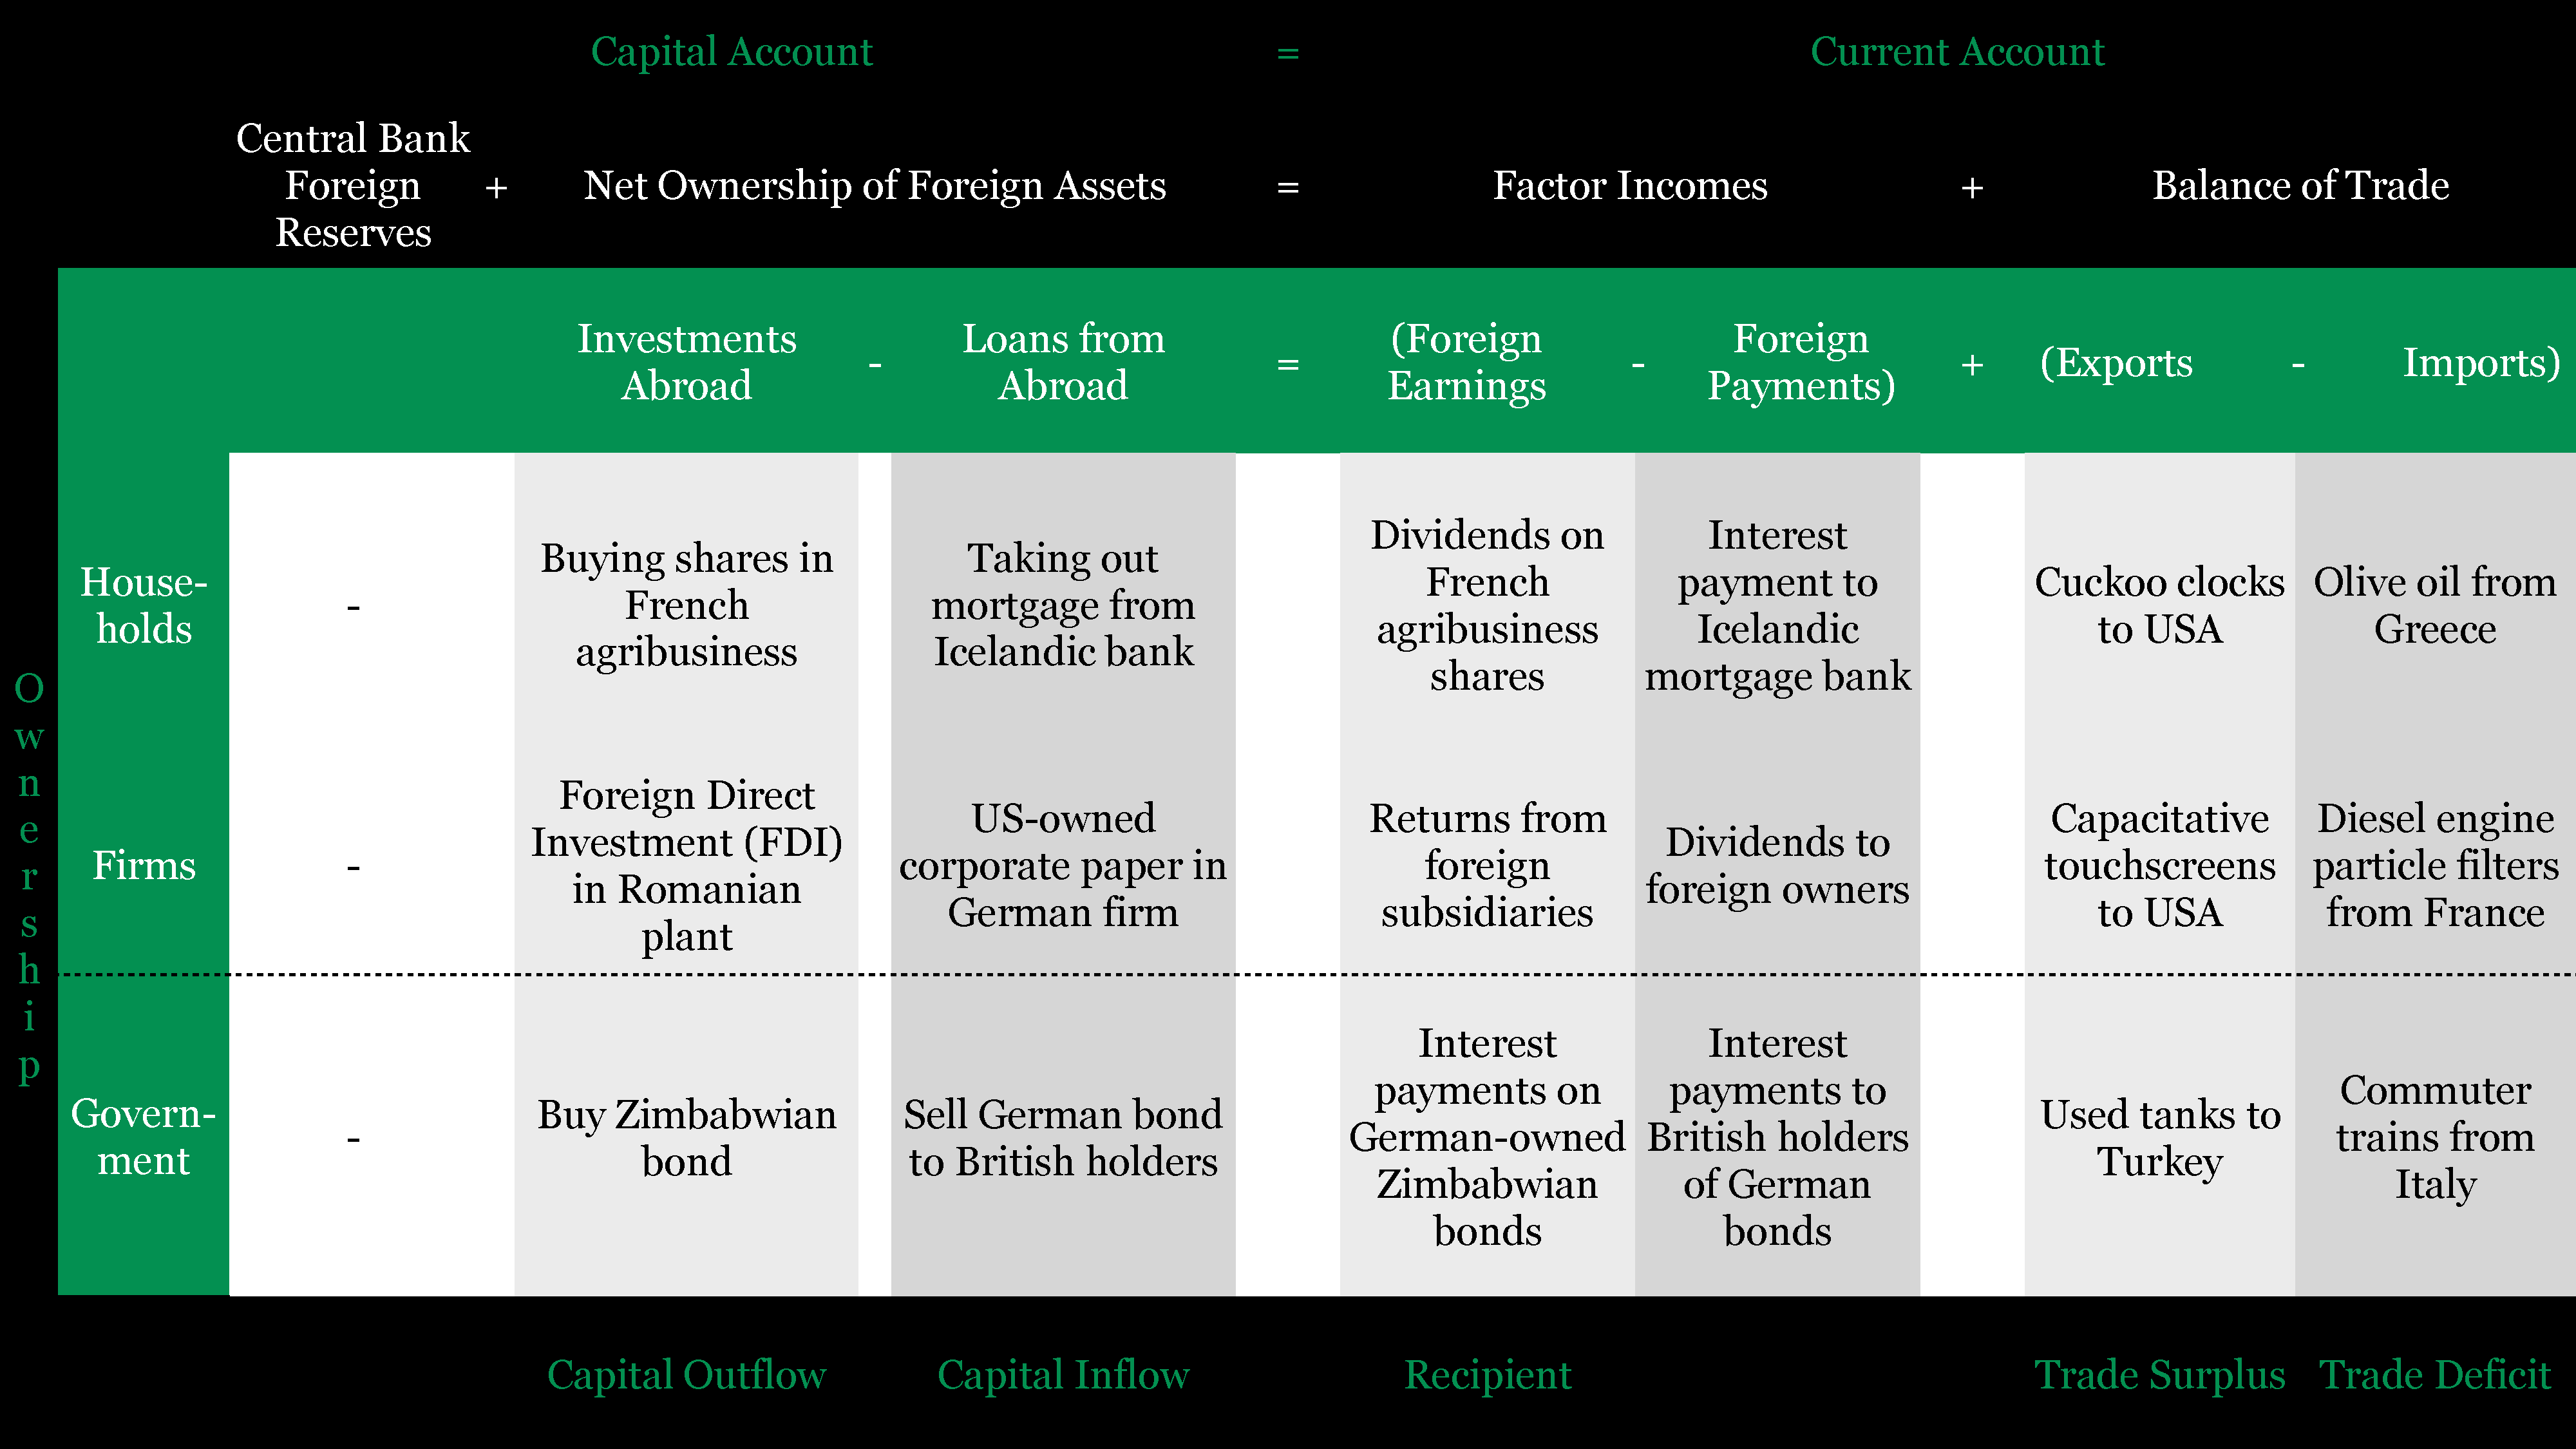
\includegraphics[width=1\textwidth]{./img/balance-of-payments}  
	\caption{A (German) Balance of Payment Account with Examples}
	\label{fig:balance-of-payments}
	\end{center}
\end{figure}

Balance of Payment accounts are easily misunderstood or oversold, for a four reasons:
\begin{enumerate}
	\item Trade deficits and surpluses between any pair of countries are frequently reported, but meaningless and entirely unproblematic, just as shoppers need not worry about a trade deficit with the local supermarket. 
	Trade deficits --- as consumer debt --- are potentially worrying only if they are \emph{net} of all exchanges with all trading partners.
	\item Conversely, balance of payments accounts do not apply  only between countries, as is easily assumed, but is, in fact a meaningful and true identity between any group of market participants and the rest of their trading partners, all the way down from nations to households. 
	For example, a trade deficit may also arise between laggard regions, impoverished demographics or even generations, and the rest of an economy, with much the same possible problems.
	\item In the short term, even such trade deficits may not be problematic, but, in fact, help to stabilize economies from exogenous shocks. 
	%reference OCA argument
	\item Even in the medium and long run, persistent trade deficits may be ok if and to the extent that the resultant capital inflows can reasonably be expected to currently, or in the future, earn whichever factor income was promised. 
	For example, emerging economies may well experience persistent trade deficits for some time, while machinery is imported to equip the workforce, if and to the extent that the resulting, now capital-deepened production pays off as expected.
\end{enumerate}

Still, balance of payments accounts are an immensely enlightening abstraction, without which trading mixed economies cannot be well understood:
\begin{enumerate}
	\item Trade deficits are not a sufficient, but still a necessary condition for building macroeconomic imbalances. 
	Not every trade deficit will betray an economy living beyond its means, but every economy artificially held above its long-term growth path by said financial drugs \emph{will} leave a grave trade deficit in its wake.
	\item The balance of payments identity shows, as Keynes  argued forcefully, if somewhat ineffectively at the Bretton-Woods conference in 1944, that these macroeconomic imbalances know no \emph{one} culprit. 
	The loaded language notwithstanding, both deficit \emph{and} surplus economies are, equally, at fault. 
	One parties excessive imports are another parties dumping exports. 
	To get to equilibrium, where imports equal exports, either of the two parties, or both, must change its prices. 
	To pride oneself, as German leaders frequently do, in being an export champion --- but not an import champion --- is but a mindless return to the folly of beggar-thy-neighbor, and, before that, mercantilism.
	\item Financial flows always track flows of tangible goods and services, as well as vice versa.
	\item It does not much matter \emph{who} --- households, firms or government --- in an economy creates the trade deficit. 
	Only the deficit net of all economic actors in a given region matters. 
\end{enumerate}

How, then, do we know the acceptable trade deficits, from the unsustainable ones? 
We look at the offsetting changes in the capital account, and check whether these are intertemporally efficient, or whether they were enabled by failed markets. 
In the \gls{EU}, as in any other mixed economy, we must beware of these smoke and mirrors, that only forestall and worsen the inevitable day of reckoning: 
credit bubbles, asset bubbles, inflationary pressure, and nominally invisible, but real dissavings.  %add hrefs.

\begin{description}
	\item[Credit Bubbles \& Default.]  Trade deficits can precipitate in capital inflow, as new foreign-held debt. 
	To receive their extra imports, deficit economies issue different forms of IOUs, including government bonds, corporate debt and household credit, sometimes backed by physical collateral, as in a mortgage.%gls IOU

	If the sum of these debts, is sound, so is the trade deficit. 
	If debts, sour, or were overly optimist to begin with, the trade deficits cannot stand. 
	Consider the two scenarios:
	\begin{enumerate}
		\item The loans are performing as long as, if, and to the extent that whichever projects they financed generate sufficient earnings to pay back interest and principal. 
		For example, if the extra, imported surplus production the IOUs enabled were transformed into a competitive factory that now churns out export merchandise, the loan can be paid be back out of these exports and revenues. 
		
		In the \gls{balance-of-payments}, the initial trade deficit is first offset by the loaned capital inflow, which later flows out again as the loan amortizes, offset by foreign factor payments and exports of the produced merchandise. 
		In effect, the loan has, as efficient credit should, inter-temporally balanced past trade deficits with future trade surpluses and/or foreign payments. 
		It matters little whether, and in which proportion the amortization on the capital account is offset by either foreign payments or equivalent actual exports, and whether the factory's merchandise is actually for export or domestic consumption. 
		In the balance of all economic transformations and exchanges, successful factories and other projects can always honor their loans \emph{without} curtailing the living standard of the population. 
		Interest, and maybe even collateral, are paid back out of \emph{extra} production that would not have otherwise occurred. 
		We need not worry about this kind of trade deficit: 
		because it moves everyone closer to the long-term growth path, is an inter-temporal Pareto, or at least Kaldor-Hicks optimization.

		\item The loan goes bad as soon as, if, and to the extent that whichever projects they financed do not generate sufficient earnings to pay back interest and principal. 
		For example, if the factory is not competitive, or --- more to the european point --- no one needs or can afford the airports, malls and mansions into which the extra imports were coagulated, there are no revenues or exports to pay back the loan. 
		In the extreme, but conceptually similar and now plausible case, the extra imports were not meaningfully coagulated into capital at all, but were simply consumed away at present.
		
		Come the day of inevitable reckoning, the deficit economies have two choices:
		\begin{enumerate}
			\item If the loan in question carries effective recourse, the deficit economy has to return the loaned capital in other, \emph{material} ways. 
			As when a leasing company repossesses a car on which payment the lessee has fallen behind, deficit countries must return the surplus production in some form. 
			For example, the deficit economy may ship back the foreign-financed machinery in the project, or, more likely, return the same amount of surplus production transformed into some other good or service. 
			
			This is the hard way of rebalancing the \gls{balance-of-payments}: 
			the inevitable, promised outflow of capital on the capital account can be balanced only with an often painful trade \emph{surplus}, because there are no factor incomes to be otherwise offset on the current account. 
			Either way, a failed investment enforces a later, and often painful trade surplus to return principal and return.

			\item Alternatively, if and to the extent that debtor economies (can) forego recourse and exert sovereignty vis-a-vis creditor economies, they (partially) default on their commitments and simply refuse to return the coagulated surplus production. 
			In that case, creditors are stuck with their claim. 
			By fiat, the original loans become full, or partial \emph{transfers} from the debtor to the creditor economies. 
			Here as always, the two sides of the \gls{balance-of-payments} identity cancel out: 
			the original trade deficit is matched by a later, ex-post, enforced, foreign payment in the form of debt forgiveness, haircut or default.
		\end{enumerate}

		No matter the choice, this kind of trade deficit is never an optimization, but an unavoidable \emph{redistribution}, either from surplus future to deficit present if and to the extent that debtors pay, or from creditors to debtors, if and to the extent that debtors default.
		
		Crucially, it matters very little who in the deficit economy --- households, firms or government --- initially took on debt. 
		These non-performing loans will redistribute from future to present, or creditor to debtor no matter who signed them. 
		In many cases, government will be forced to act as the lender of last resort and take on, or guarantee all the bad loans, both to counteract adverse selection and, often to save an exposed banking system from systemic crash. 
		Even if and to the extent that government, or, equivalently, future taxpayers, can avoid to take on the bad loans, the redistribution is merely concentrated on whoever remains nominal debtor. 
		Domestic policy can force only \emph{some} people --- ideally those responsible --- to repay, but, short of default --- another redistribution --- it cannot void the need to repay. 
		Here, as always, something akin to economic conservation of matter reigns: 
		when credit bubbles burst, someone will have to pay back the future, either some debtors, all taxpayers, some creditors, or any combination thereof.
		
		In addition to these mere inter-temporal distributions, credit bubbles and associated mass defaults or austerity, of course, also waste economic welfare, because of the turmoil they harbor, not to mention the hardship they imply. 
		As the business cycle fluctuates wildly in such crises, the economy diverts from the long-term growth path, leaving resources either depressively idle, or manically scarce.
		
		Credit bubbles are a market failure that may plague any economy --- not just the \gls{EU} --- but the european, defunct mixed economy is particular prone to them, for at least three reasons:
		\begin{enumerate}
			\item The \gls{EU}, until at least 2012, exercised most macroprudential oversight and otherwise mostly regulated financial markets at the \gls{MS} level. 
			Here, even the regulatory arm of the mixed economy was impaired, and regulations might have been arbitraged to subalance-of-paymentstimal levels. %find source.
			\item Monetary policy drives bank lending. 
			The \gls{ECB}, because it can set only \emph{one} monetary policy, was unable to react to credit bubbles in individual markets or regions, such as Spain or Greece. 
			\item Equivalently, if there were in the \gls{EMU}, or ever hoped to meet the its nominal convergence criteria, deficit and credit-crazed \gls{MS} also could not devalue their currency through monetary interventions.
		\end{enumerate}
	\end{enumerate}
	
	\item[Asset Bubbles \& Crashes.] Broadly similar, and often concomitant to credit bubbles, asset bubbles can also fuel trade deficits. 
	As some assets in the deficit economy are persistently overvalued, foreign investors buy up these domestic assets, offsetting the trade deficit on the current account with a capital inflow on the capital account. 
	Real estate, stock or some other asset that did not previously exist, or belonged to domestic investors, changes hand to foreign investors, expecting an ex-post unreasonable return. 
	Come the day of reckoning, asset prices plunge, and much the same process sets in as when credit bubbles burst, only in asset bubbles, the default incidence is on the foreign investor, because she will usually, if not always, have taken risk-bearing equity in the asset. 
	
	Asset bubbles, too, are a redistribution from a future day of reckoning to a manic present, and, in that future, a redistribution from foreign investors to the domestic economy. 
	In addition, asset bubbles also waste welfare: 
	when they burst, they spiral downwards, often cause grave systemic risk and generally divert the economy from the long-term growth path.
	
	Asset bubbles, too, are a universally looming market failure, but the \gls{EU} is particularly vulnerable, again, because of likely regulatory arbitrage and ill-fitting monetary responses to local business cycles.%add href.
	
	\item[Monetary Expansion \& Inflation] Overly expansive monetary policy can also enable unsustainable trade deficits. 
	In this scenario, central banks simply inject more fiat money into the economy to offset the current account deficit with a Potemkin inflow of capital. 
	Fiat money, of course, never creates capital, and if, when and to the extent that this bluff is called, inflation ensues: 
	money supply and demand equilibrate at new, higher price levels. 
	
	This problem is widespread in the \gls{EMU} with asynchronous business cycles, a single interest rate target and no transferred stimulus to speak of. 
	In those regions where a low interest rate pumped too much money into the economy, as now appears to have been the case in Ireland, Spain, Portugal and Greece preceding the 2008ff crisis, loose money silently credit and asset bubbles, and might have already built yet-to appear inflationary expectations. %I really don't know what I'm talking about, here
	%Need data.
	
	Inflation, here, as always, wastes resources and redistributes arbitrarily. 
	%add /href.
	The middle class and older people, with frequently nominal denominated assets (pensions), but real denominated liabilities (rents) will be particularly vulnerable to whichever level of inflation this crisis might, eventually, bring.
	
	Inflation, too, as the other temporary diversions from the long-term growth path, redistributes from the future to the present. 
	Even inflation does not spiral to double-digits or more, \emph{any} additional increment in medium-term inflation and expectations is costly, as disinflating to previous levels is painful and often causes prolonged unemployment. %add source. %reference 70s disinflation
	
	\item[Dissaving \& Depletion] Trivially, economies can also go into unsustainable  trade deficits by real dissaving. 
	Instead of, say, selling shares in domestic companies, the deficit economy can just burn more of strictly limited fossil carbon, diminishing its real, if not its nominal assets.
	
	Because such real assets, including an economies infrastructure, demography, environment or CO2e levels as unresolved commons have no defined ownership rights, they do not nominally show up in the capital account of an economy. 
	Whatever this assets are transformed into, however, may well show up as an export in the current account. 
	For example, a deficit economy can dig into its coal and iron ore resources, transform them, and export them as steel, offsetting other imports. 
	Because the dissaving in natural resources is not usually recored, and thus triggers no change in the capital account, the steel export revenue will erroneously be attributed as a domestic \emph{income} in full, when in truth, much of the revenue comes from dissaved domestic assets, that ought to be recorded on the capital account.
	
	Such dissavings --- by definition --- redistribute from the future to the present. 
	As dissaving most easily and nominally invisible occurs out of vulnerable commons, it also wastes the welfare of some of our most precious, communal resources. 
	If, when and to the extent that they are depleted to sustain trade deficits, we may never or only at great cost be able to restore them.
\end{description}%might need to strengthen the crisis and imbalances components in the above.

I cannot marshall evidence here to show how each of these dynamics caused the 2008ff Euro, let alone the broader sovereign debt crisis. 
Nor can anyone, in 2012, reliably predict which of imbalances may yet turn out to be unsustainable, and why. 
What I do claim here is that whatever the actual imbalances and crises of the embattled \gls{EMU} and \gls{EU} are, or will be, they will, underneath it all, follow these scripts. 
Using some economic imagination, \emph{these} are imbalances and resulting periodic crises we would expect to plague any such internally open, but dysfunctional mixed economy.

While this european mixed economy may be of its own kind, the market failures that enable these imbalances and trigger the resulting crises are in no way \emph{sui generis}. 
The herding and information externalities that inflate asset and credit bubbles, the systemic chain-reactions that loom on large defaults and the tragic commons depleted by real dissavings are the kind of market failures that plague all real-existing capitalism. 
As such, they must be meet the appropriate regulatory, fiscal, and --- to a lesser extent --- monetary responses. 
%add \href
Similarly, loose money tempts governments of all market economies, not just --- in fact, probably, least of all --- in the \gls{EU}. 
It, too, must everywhere be curtailed by policy: 
a constitutionally-enshrined monetary governance, preferably a robustly independent central bank, bound to a well-defined goal. 
Because as dangerous drugs endemic to capitalism, these problems are not European problems, they also do not require a European solution. 

Still, the deficient european acquis exacerbates the imbalances and crises looming everywhere, in at least three ways \citep[echoed by][25]{Bordo2011}:
\begin{enumerate}
	\item Without a monetary union or nominal convergence criteria thereto, trading economies can intervene in their exchange rate, or, at least, let their currencies depreciate freely. 
	As adjustment mechanisms, none is as fast as currency devaluation to get out of trade deficits. 
	In an instant, imports become more expensive and exports become cheaper, ideally, until import and exports equilibrate at the free exchange rate. 
	Alternative --- and ultimately equivalent --- domestic readjustment of (higher) prices and (lower) wages often takes longer, maybe too long to avert a \gls{balance-of-payments} crisis. 
	
	Discretionary exchange rate interventions are difficult to get right, and easily deteriorate into competitive devaluation, or beggar-thy-neighbor by a fancy name. %add source. 
	Freely fluctuating exchange rates, in turn, are costly as the second theory of optimal currency areas reminds us, %add source
	and they, too, might be the result of herding or otherwise failing global currency markets.
	
	As drug addiction therapies goes, the methadone of devaluation is, at best, a mixed blessing.
	
	And still, it is a prescription, the european economy has to do without, no matter the indication. 
	Within the \gls{EMU}, everyone in the \gls{EU} who ever wants to join, currencies cannot fluctuate. 
	To readjust, member economies can only hope their wages will not be too downwardly sticky.
	
	\item Creditors and debtors alike will anticipate the systemic risk and spillovers that the monetary union bestows on all its members. 
	They know that other members too, would suffer from defaults or, related, \gls{EMU}-exit, and, therefore, will likely bail them out. 
	%add more stuff here, why is that so? I wrote that somewhere.
	With systemic default risk as a union-level commons, but decisions in individuals, firms and, at best, \gls{MS}-hands, credit everywhere, but particularly in the high-risk economies, will be too loose.
	
	The \gls{EU}, in other, metaphorical words, is not only plagued by powerful and addictive drugs, but dealers and addicts alike can reasonably expect to be saved --- as the should --- if they overdose.
	
	\item Lastly, and familiarly, the european mixed economy lacks the fiscal means to otherwise rebalance internal demand, that intact mixed economies use to mitigate regional imbalances, including public works, industrial policy, or even straightforward transfers.
\end{enumerate}

The imbalances that have built up over the last years of European integration, and the crises in which they now seem to erupt, tell of the market failures of our capitalist economy. 
But they also betray the underlying dysfunctions and unfairness of an impotent mixed economy, that built these pressures in the first place. 
To bemoan only the market failure, and to seek to redress it is as naive as it is dishonest. 
Even worse, to simply wish away the crises, and to blame someone (``the banks'') --- \emph{anyone} (``'the markets'') for our misfortune, is to shoot the messenger, rather then to heed her warning.

In drug policy, if you are faced with a rampant substance abuse, you have to follow \cite{Mills-1959-aa}, and sociologically re-imagine the saddening observation of an overdosed corpse: 
you have to ask how, and why, people socially turn to harmful drugs in the first place, and then, if you can, cure this anomie, whatever it may be. 
If you only wage a war on drugs, they will always win.

And so it is with the imbalances and crises facing the \gls{EU} today: 
we have to use our economic imagination to explain how, and why, the european economies turned to delusional market failures in the first place, and, if we can, strengthen them to resist any siren call. 

Our anomie, now, should be clear enough: 
it is the underfunding, unemployment and inequality left untouched by an impaired command arm, that slowly, but steadily, unravels the social contract of the mixed economy. 
Faced with such pressures, it is little wonder that individuals, firms, states and the household-writ-large they collectively make up turn to the sirens of delusional growth.

Boxed in, as it is, the dysfunctional mixed economy, and especially its poorer constituents, find ways to relieve such economic pressure \emph{somewhere}, to postpone such austerity to \emph{somewhen} and disguise such anomie \emph{somehow}. 

To now, as many do, deplore only the failing markets
\footnote{
	For some social science that seems to physically placing ``markets'' in quotation marks, see, for example \citealt{Beckert2012}. 
	In lieu of an economic, or social scientific explanation of failing or corrupted markets for sovereign debt, this rhetorical device works to distance the social scientist from these market messengers, as if their price signals were merely social constructs. 
	There is, however, such a thing as objectively given, materially tangible, unsustainable debt that higher interest rates might merely communicate \citep[55]{Wihlborg2010}.
	 ``Punctuation'', in any event, does not replace an explanation.
}, 
to demonize investors or politicians is an act of exorcism. 
It was \emph{we}, who made a Faustian bargain with these devils: 
to let them reign free, if only they could numb the economic pain. 
They obliged us. But no one, as Doctor Faustus, should be surprised if some day, there is hell to be paid.

\subsection[An Old Deal]{An Old Deal} %or: why it matters

\begin{quote}
	\emph{``We can't start another new deal.''\\
	``How about fighting for the old one [...]?''\\}
	 --- The West Wing (Season 5, Episode 5), created by Aaron Sorkin.
\end{quote}

To insist on an intact mixed economy is not so innovative. 
The mixed economy is, in fact, a very old deal, prepared by the social reforms of Chancellor Bismarck, forged by Presidents Roosevelt and Truman, institutionalized by Lord Beveridge and, with miraculous success, reactivated in war-torn Germany, by Chancellors Adenauer and Erhardt. 
If there is such a thing as a European social model, or really, \emph{any} capitalist social model, it is the mixed economy.

To insist on an intact mixed economy is also not radical. 
The mixed economy, is, at heart, a compromise of exchange and command, of market and state, of individual freedoms and duties, of efficiency and equity. 
The mixed economy hopes not for an end of history, nor harbors any overhaul of society: 
it makes amends with capitalism.

Tax --- the cornerstone of the mixed economy --- in particular, is a reformist, never a revolutionary project. 
Good taxation, especially of consumption, accepts private property as given, even legitimate and desirable, and merely adjusts the sticks and carrots that people reap for their personal enjoyment. 
Minimizing their \gls{DWL}, good taxation maximizes the freedom of all market participants to do as they would \emph{absent} the tax.

Today, Europe is reneging on this old deal. 
Without union-level taxation to speak of but with full factor and goods mobility, tax schedules are compressed and levels lowered. 
Without fiscal complements, the common currency allows imbalances and lets diverging business cycle fluctuate widely. 
Even regulation is yet incomplete, such as in labor market legislation, and is arbitraged away by competition. 

On these institutions rides it all: 
that we can efficiently produce public good cancer research or preserve our environmental commons, that we can pool the risks of the healthy and the frail, that we can restore some fairness between market winners and losers, that our children will receive at least what we have received, and that our neighbors prosper, too. 
%add hrefs
Tax especially, and together with regulatory and monetary institutions, \emph{are} the social contract of modern capitalism. 
%add source

European regional integration does not rewrite the social contract, but sins by blithely omitting much of passages on tax, monetary and regulatory policy. 
Absent them, the european polity is no longer free to choose between %add old graph
command and exchange, but --- without explicit popular consent --- defaults to ever more market, and ever more present consumption. 
Our household-writ-large now occupies a greatly constrained coordinate space (figure \ref{fig:coordinate-space-constrained}), boxed in by chronic underfunding,  looming unemployment and rampant inequality, shaken by recurring imbalances and crises. 

\begin{figure}[htbp]
	\begin{center}
	\includegraphics[width=1\textwidth]{./img/coordinate-space-constrained}  
	\caption{Constrained Coordinate Space of a Dysfunctional Mixed Economy}
	\label{fig:coordinate-space-constrained}
	\end{center}
\end{figure}

By its dysfunctional design, the european mixed economy yields ever more to markets while the other part of the mixed economy, the state, is on the retreat. 
Bereft of their old, flexible and capable social contracts, the acquis will, nay, already \emph{has} --- however fortuitously --- remade european society in the neoliberal, consumerist image. 
``Neoliberalism'' and ``consumerism'' are, in this case, not catch-all labels of disaffection, but I choose them with equal anger and care, and they apply precisely. 
The aquis is:
\begin{description}
	\item[Neoliberal,] because, eviscerating the state, it morphs markets from one of several \emph{means}, to inescapable \emph{reality} or even ultimate \emph{end}, neither of which it is, nor should be.
	\item[Consumerist,] because, it cannot set a positive savings rate, and leaves austere members no choice but to loot real savings, and give into the temptations of bubbles. 
	As a result, much of the resources of the communal household will be devoted to near-term consumption
	\footnote{
		The \gls{EU} commission is quite explicit about this:
			\begin{quote}
				\emph{``The Single Market Review put \emph{(sic!)} citizens, consumers and \glspl{SME} at the centre of policy-making.''}\\
				--- \cite[3]{Commission2008}	 
			\end{quote} 
		One wonders, at least, why, in addition to \emph{citizens}, consumers and \emph{some} (though not other) firms are also mentioned, when, in a functioning market, the latter two should be served only as proxies of the ultimate beneficiary, the citizen.
	}.
	
\end{description}

Just how angelic the postwar mixed economy really was, I do not know
\footnote{
	To mention just a few red flags, it is unclear what costs Postwar prosperity extracted from others (dependence or world systems theory), we do know whether or how Western affluence can be repeated without the same gigantuan carbon footprint and we worry whether broad-based growth in value-add is but a historical episode (cost disease).
}. 
Still, \emph{relative} to 19th century mass poverty \citep{MarxEngels-1848-aa}, 20th century ``mob politics'' \citep[158]{Crouch2004} and the spectre of 21st century neo-laissez-faire, the mixed economy, and the welfare state it has enabled, appears as singular achievements of the modern era. 
The economic institutions of Postwar Western Europe have brought about unseen prosperity and equity, all in relative peace and freedom. 

That is an old deal worth fighting for.

\subsection{Catch-Up}
\begin{quote}
	\emph{``Three tomatoes are walking down the street --- a poppa tomato, a momma tomato, and a little baby tomato. 
	Baby tomato starts lagging behind. 
	Poppa tomato gets angry, goes over to the baby tomato, squishes him, and says: catch up.''} \\
	--- \href{http://www.youtube.com/watch?v=5D-QKY0-Bxk}{Mia Wallace in Pulp Fiction (1994)}
\end{quote}

	%Another perspective in favor of EU tax competition construes different tax rates as an essential component of the comparative advantage at play in European integration. 
	%There are different variations on this argument.
	%László Kovács (2004), then Commissioner for Taxation and Customs asked that tax rates must be allowed to differ 6-8% simply to make up for the remote location of some markets.
	%More broadly speaking, tax competition could be construed as convergence "through the back door", enabling small and relatively poor countries to catch up faster than they otherwise would-

	%Parallel to the optimum currency debate, non-harmonized, competing taxes can serve states to more flexibly respond to asymmetric shocks. 

	%Lastly, it could be argued that the EU, given its wide economic opening to the rest of the world, is playing a Prisoner's Dilemma at another, global level, too. 
	%Even subalance-of-paymentstimally low tax rates would then be individually rational for the EU to pursue, and internal tax competition could be regarded as either inconsequential or desirable to "defect well".


	%Tax harmonization has dramatic redistributive potential between the union's member states. 
	%Construing tax competition as convergence through the back door points in this direction already: small and poorer countries stand to loose from tax harmonization, as evidenced by their opposition to EU tax cooperation (Kellermann & Kammer 2009: 138).
	
	
	%In an extremely asymmetric configuration, it may be the case, that tax coordination becomes a zero-sum (rather than positive-sum Prisoner's Dilemma), where harmonization only redistributes wealth to the richer and larger states.

	%Harmonized, more progressive tax rates across the European Union 	will reduce the competitive advantage of emerging markets. 
	%This is an unavoidable redistributive trade-off.
	%A feasible tax harmonization would still require different real tax rates, so as to account for  lower factor productivities in less developed economies. 
	%The ultimate goal for tax harmonization should be roughly equal post-tax factor prices, weighted by factor endowments with equal progressions everywhere in the Union. 
	%That would define the absence of any tax competition; given such a degree of harmonization, the EU (under autarky) could set arbitrary tax rates and progression schedules.

	%Such harmonized taxation - all other things equal - would slow down the growth of emerging markets dramatically, rendering it a similarly bleak outlook in terms of sustainability as race-to-the-bottom tax competition
	%Economically less developed member states are unlikely to ever agree to this.

	%To counteract this effect, a harmonized tax system must be accompanied by substantial fiscal redistribution between the member states, in other words: fiscal federalism, with large "eastwards" transfers to hasten convergence along. 
	%There are good normative reasons to favor tax harmonization. 
	%The continent's integration requires progressive schedules to strengthen social cohesion, further employment and redistribute the unions' fruits. 
	%The throes of transition, and building of a sustainable, prosperous (think: Lisbon Strategy) future require well-funded governments that can dampen shocks and invest wisely and substantially. 
	%Tax competition must be overcome, because it is both inequitable and inefficient in the longer run. 

	%Some of the arguments against harmonization-cum-redistribution are mistaken. 
	%Given widely available and sophisticated economic statistics and the experience of domestic fiscal federalism, some (surely imperfect) redistributive compensation does in fact seem technically doable. 
	%Moreover, harmonization-cum-redistribution does not necessarily imply a larger public sector overall: it is conceivable and preferable at any level of public spending. 
	%While it does imply a larger public expenditure quota particularly for NMS, this need not be equated with greater, potentially undesired provision of public and common goods. 
	%If preferred, electorates can choose to channel the side-payments to private consumption.

	%If tax competition and a move to regressive, immobile bases is happening, as it appears, it has very real consequences on the life-chances of the economically disadvantaged. 
	%Similarly, the growth trajectories of the NMS have very dire implications for the wellbeing of everyone, and particularly the poor in those countries. 
	%The downsides of both tax competition and harmonization have a social gradient, in other words. 
	%By naturalizing the inevitability of the status quo, this working group ignores the questions of distributive justice which ultimately underly any choice or non-choice of how to do economic liberalization. 

	%Moreover, by inducing more economic hardship, structural unemployment and fiscal imbalance, the very concerns about what the EU can reasonably achieve may put in danger the prospects of unification.

	%Harmonized taxation cum fiscal federalism will allow the European Union to grow, wide and deep, not just "united in diversity" but "integrated in cohesion".


Too easily, discontent with a retrenching Western European welfare state blames \gls{CEEC} ``social dumping'' %source
or otherwise slides into poorly disguised economic nationalism. 
It must not: 
whoever thinks that Western and Northern, otherwise intact mixed economies now whither away because of competition from the East and the South, misunderstands, or --- more likely --- misconstrues the issue.

Of course, the newly opened, low-productivity and low-capital markets in the poorer East and South have much lower, often proportional taxation, especially on capital incomes. 
They \emph{cannot} afford high, or progressive taxes on capital, if they are to remain competitive, let alone converge
\footnote{
	For example, L\'{a}szl\'{o} Kov\'{a}cs (2004), then Commissioner for Taxation and Customs asked that tax rates must be allowed to differ 6-8\% simply to make up for the remote location of some markets.
} 
Had Romania the capital income taxation of pre-reform Sweden, the net returns on any investment would fall tremendously. 
Given the low labor and total factor productivity in Romania, an investment might not be profitable at all, and capital might instead stay in high-tax, but also high-productivity Sweden. 
Romania would not be able to attract much foreign capital, which it so direly needs to leapfrog into convergence.
	
By contrast, the high-productivity, high-capital markets in the West and North, \emph{could} afford higher, and more progressive taxes, if only they did not face tax competition from all other \gls{MS}. 
Had Sweden the capital income taxation of post-accession Romania, or even the 0\% \gls{CIT} of non-member Moldova \citep{Piatkowski2008}, it would have to abandon much of its mixed economy. 
Forced to finance its large public sector only out of labor, or other immobile, proportional sources, the tax wedge on the lower and middle strata of society would become unbearable. 
%add \href

At first sight, there appear to be only two policy responses to this conundrum:
\begin{enumerate}
	\item \emph{High European-Level Taxation.} \gls{MS} might agree to enforce union-wide, uniformly high and progressive taxes on mobile bases, that would save welfare in the rich \gls{MS}, but at the cost of laggard growth in the poor capital-deprived \gls{MS}. 
	Such tax cooperation would save the welfare state, but sacrifice fast, or even any, convergence.
	\item \emph{Tax Competition.} \gls{MS} might continue with the status quo ante, set tax rates individually and let competition whither away levels and progressivity. 
	Such tax competition would sacrifice the welfare state, but bring some convergence ``through the back door'' as rich \gls{MS} capital will to rush to poor \gls{MS}: 
	poorer (and smaller) countries win under tax harmonization, as evidenced by their opposition to even nascent \gls{EU} tax cooperation \citep[138]{Kellermann2009}
	\footnote{
		Capital inflows will be particularly effective in relatively poor economies. 
		As these economies, supposedly, still lie far below the golden rule of saving \citep{Solow1956}, returns on capital will be much higher than in richer economies where further (near-Solowian) capital deepening faces diminishing returns (e.g. \citealt{Barro1995} or \emph{ibid.} 1992 as cited in \citealt[3]{Beckfield2009}).
		}.
\end{enumerate}

Such are the alternatives that politicians might peddle, pitting poor members against rich, convergence between them against welfare within. 
These are, as so often in defunct mixed economies, impossible choices to make, seemingly forcing European democracies to play a game of zero-sum.

Alas, regional economic integration, as all trade, is not zero-sum game: 
there are gains to be had, if not accruing to everyone equally. 
Sweden is better of for having a prospering, converging Romania as a trading partner, with different absolute or comparative advantage, capital endowments and areas of specialization. 
Out of the proceeds of this positive-sum game, there is a third option:
\begin{enumerate}
	\setcounter{enumi}{2}
	\item \emph{High European-Level Taxation With Side Payments.} \gls{MS} agree to enforce union-wide, uniformly high and progressive taxes on mobile bases, but rich \gls{MS} recompense poor \gls{MS} for their ensuing competitive disadvantage. 
	Absent different taxes rates on mobile factors, the union as a whole is able to choose freely amongst the tradeoffs of a mixed economy, including a well-funded welfare state. 
	Still facing low labor productivities, poor \gls{MS} receive fiscal transfers that they can use to build capital stock, educate their workforce, upgrade infrastructure, or even subsidize investment. 
	For example, poor \gls{MS} might lower or even abandon taxation of some or all immobile factors, such as low-productivity labor. 
	Facing a small or no tax wedge, maybe even receiving subsidized or free health care, or some other \gls{NIT} of sorts, the low-productivity workers in poor \gls{MS} would be able to accept yet lower gross market wages, and become competitive again, even as investors have to pay high taxes
	\footnote{
		To remind readers that this is not, in fact, what the acquis currently stipulates: 
		The overall structural and cohesion funds for 2007--2013 amount to no more than \euro 347 billion, less than 3 times the budget of the city of Berlin (\euro 21 billion in 2009), or about 0.005 \% of the budget of Germany (\euro 1,164,000 billion in 2011). 
		In addition, \gls{EU} budget negotiations are still marred by \emph{juste retoure} attitudes, with \gls{MS} wanting to get paid out what they have received --- the very opposite of a redistributive regime \citep[e.g.][]{Begg2008a}.
	}.
	
	Side payments need to be initially large enough but decrease over time, and they must be used wisely by poor \gls{MS}. 
	As in any subsidy or  protection, it will be difficult to avoid long-term dependence and rent-seeking.
	
	If we get it right, though, high european-level taxation with side payments will save the mixed economy, enable a potent welfare state, clear factor markets, converge living standards in the union and keep us all on the long-term growth path. 
\end{enumerate}

%add game theory here. 
%Is there a game to be played? %create a table about the options in the catch-up game.

We need not trade off openness and convergence \emph{between} \gls{MS} with efficiency and equity \emph{within} them. 
In fact, they are the same issue: 
behind the pressures on rich welfare states always lurks the question of convergence: 
just how fast, and by which means, do we want the poor members to catch up?

If we opt for policy response \begin{inparaenum} 
	\item high european-level taxation, convergence will be minimal and through the market only. 
	If \item we choose tax competition, convergence will be faster, and still only market-led. 
	If we \item adopt high european-level taxation with side payments, convergence can progress at an arbitrary speed, with a substantial state component. 
	\end{inparaenum}

Deciding on the speed of the catching up may just be the deeper question of european integration that many politicians of all colors, but especially those tending to economic nationalism, may seek to avoid by misrepresenting european choice in dichotomous terms of more or less protection, more or less integration. 
Convergence supported by side payments \emph{does}, of course, include a zero-sum component, as any redistribution by definition does. 

But it is not, as it is easily made out to be, redistribution \emph{between} one economy and another, it is instead, redistribution \emph{within} one, European economy. 
Whenever the markets expand beyond borders, so, too, the abstractions of the mixed economy rule at a higher level, and they apply not just to tax --- the clearest case that I have here illustrated --- but to all command interventions prone to arbitrage: 
as the first good, service, or capital equipment crosses the border, the two trading partners have already adopted \emph{one} of the three regimes of economic integration, and, related, have made their however implicit choice of just how, and how fast, the poorer party gets to catch up.

The elephant in the room of european economic integration is this: 
if we are to save the mixed economy, we have to explicitly decide, not just agree by default, how fast we want to converge
\footnote{
	It too, is neither new nor revolutionary: 
	internally heterogenous mixed economies have always, with varying results, dealt with this question. 
	In the US, much of the controversy about the role of the federal government boils down to the question of how much rich Texans should dole out to poor Louisianans. 
	In Italy, the rift is between North and South \citep[e.g.][]{PutnamLeonardi-1993-aa} and in Germany, initially between industrial and rural states, since 1990 between old and new \emph{Laender}.
}.

\section{Who Dunnit?: Second-Order Theory of Negative Integration} \label{sec:who-dunnit}

So, a reader may ask, what does any of this have to do with who, or what  ``built welfare states in post-communist \gls{CEEC}'', or alters them elsewhere in the \gls{EU}? 

The defunct mixed economy of the \gls{EU} has everything to do with the continents welfare states, not just because in the East, the \gls{EU} (and \glspl{IFI}) might have --- and still do --- dictate economic policy to any country who might ever wish to join the union through convergence criteria, accession negotiations and conditionality \citep[55]{Bonker2006}, but because, much, much more fundamentally, any economic or social policy adopted in \glspl{CEEC} after 1990, or elsewhere, is greatly constrained by the European economic regime in place. 
\gls{EU} regional economic integration, to be sure, only dictates what cannot be done: 
no progressive or high taxation, no independent monetary policy, and, sometimes, no effective regulation. 
%add hrefs
European integration, in \citeauthor{Scharpf1997}'s influential formulation, is \emph{negative integration}, but nonetheless consequential \citep{Scharpf1997}. 
If there is anything to the otherwise muddled empire thesis \citep{BeckGrande-2007-aa} it is this: 
cripple your mixed economy and settle for the promises of neoliberalism and consumerism --- or perish in autarky.

I do not know, nor claim to explain here, who committed this ``perfect crime'' \citep{Galbraith2002a} --- but murder of the mixed economy, it was, and that is the deed that any second-order theory of social change has to explain.

\subsection[Literature]{The Testimony: Critique of the Literature} \label{sec:Literature}

\begin{quote}
	%\emph{``Abstraktion, das Denken in Systemen wurde durch das jeweils Unmittelbare, das Pragmatische ersetzt. 
	%Damit haben sich die sozialdemokratischen Parteien Zug um Zug desavouirt.''}\\
	\emph{``Abstractions, thinking in systems has been replaced by the immediate, the pragmatic. 
	This is how the social democratic parties have disgraced themselves.''}\\
	--- Herbert \cite[41]{Schui2009}
\end{quote}

On that count, some of the literature falls short: 
it fails to bring the \citeauthor{Mills-1959-aa}ian sociological imagination and \citeauthor{Keynes1936}ian economic abstraction to bear on the nitty-gritty empirical data of \gls{CEEC} and other welfare reform, to even discern  the offense to the post-war social contract. 
%add footnotes to authors.

This blithe ignorance comes in at least four different flavors, that I here summarize as follows:
\begin{enumerate}
	\item \emph{TINA}-flavored literature holds that the mixed economy expired unavoidably and therefore, requires no further investigation. 
	For TINAs, the mixed economy is not murdered, but dies a natural death.
	\item \emph{Pangloss}-flavored literature accepts possible alternatives to death, but assumes that, axiomatically, it was the best possible course of action, and therefore acquits any possible suspect. 
	For modern-day Panglosses, the defunct mixed economy is collateral damage to a worthy cause.
	\item \emph{Newsspeak}-flavored literature shrouds itself in impermeable and misleading language. 
	For newsspeakers, the mixed economy is not dying, but just ``restructuring'' into less complex organic compounds (known as ``decay'' in oldspeak).
	\item \emph{Bystander}-flavored literature abstains from judgment, or even conclusion. 
	For bystanders, it may or may not be murder, but it's none of their business. %add hrefs to below sections
\end{enumerate}

\subsubsection{TINA}

\begin{quote}
	\emph{``There [\ldots] is no alternative.''}\\*
	--- Margaret Thatcher (London, 1980)
\end{quote}

TINA is hardly observed directly in the literature, if only because, as a political strategy, it aims to ``veil the essentially political character of political decisions'' \citep[314]{Bluhdorn-2007-aa}, and therefore, will not even explicate itself. 
The purported lack of alternatives, mostly, asserts itself not by negating existing alternatives, but by ignoring them.  

Evidence of TINA, therefore, lies mostly in conspicuous omissions, the most glaring of which is that no literature I am aware of even acknowledges a hypothetical scenario in which \gls{EU} trade liberalization co-occurs with strong redistributive and stimulus policies, and how such wide \emph{and} deep integration might have played out. 
Such a mode of concurrent economic and political integration even has a recent historical precedence of integrating a \gls{CEEC}: 
German reunification --- however flawed in its implementation, or disappointing of its promises --- not only introduced economic and currency union in 1990, but, simultaneously, politically integrated the new L\"ander and launched a massive fiscal expansion, including an expressly redistributive ``solidarity surcharge'' tax. 

TINA is also elusive, because it has become so successfully omnipresent, that we hardly recognize it anymore, where it lingers. 
For example, when \citeauthor{Kovasc} speculates that ``Eastern Europe may be unlucky (...) if it is confined to imitation'' of Western European welfare states, because in the future ``these regimes will probably not produce the same performance levels as they do today'' he silently implies that such doom would be inevitable, which clearly, to a social scientist, it must not be, for it would not require any social science if it were, in fact, akin to a law of physics.  

Proponents of Western welfare states can also be conspicuously silent on some true alternatives, and tradeoffs. 
Social-democratic \cite{Scharpf1997} accepts that ``the economically less developed \gls{MS} simply could not afford [\ldots] the same level of welfare [\ldots] [as] the highly developed \gls{MS}'' but, oddly, ignores its alternative: 
transnational side-payments alternative in a european transfer union \citep[26]{Scharpf1997}. 
This silence might have been (mis)read by \cite[619]{Moravcsik-2002-aa} as \citeauthor{Scharpf1997}'s supposed preference for domestic over transnational redistribution. 
Surely, \citeauthor{Scharpf1997} is not an economic nationalist, but he does seem to throw up his hands as he concludes that \emph{either} rich welfare states or emerging economies must perish, and that, in any event, harmonization would be ``probably impossible'' \citeyearpar[26]{Scharpf1997}. 
That is the kind of despair that TINA always inspires, because it renders invisible the magnificent ability of intact mixed economies to smooth over even such epic transformations. 
It is strange and confusing that \citeauthor{Scharpf1997} --- who talks about (fiscally subsidized) German reunification (\emph{ibid.}) ---would not even mention the tax-cum-sidepayment solution to european integration, and this slight unnecessarily impairs his otherwise clear analysis. 
Ominously, \citeauthor{Scharpf1997} seems to have made amends with TINA when he commands ``\emph{normative} (sic!) political theory as well as political practice [to] come to grips with the conditions (sic!) of `democracy without omnipotence' '' \citeyearpar[29]{Scharpf1997}
\footnote{
	As happens when you fraternize with TINA, (some of) the policy prescriptions fall short. 
\citeauthor{Scharpf1997}, for example, advocates wage earner funds (pay in equity) to counteract the shifting terms of trade between capital and labor, a mostly notional innovation that might still imply real wage cuts and push more risk on possibly unwilling or unable workers. 
	He also promotes a shift to consumption taxes in the face of crumbling income and corporate tax revenues, a move that, if those taxes are prepaid, and therefore regressive will burden workers, low- and middle-income earners with the load of welfare state financing.  
	Most surprisingly --- and nonsensically --- he also seems to ask for a privatization and voucher model of health care (and other risks!), that, aside from all the possible market failures and distributive vagaries, will not in itself right the welfare state. 
	Finally, \citeauthor{Scharpf1997} even falls for the old social-democratic smoke grenade of ``parity'' contributions to social insurance, nominally shared by employees and employers, but whose incidence really always falls entirely on labor (all of the above \citeyear[30-34]{Scharpf1997})
}.

Sometimes, the TINA fallacy reveals itself with no shame, for example when \cite{Grow2005}, wondering how to strengthen the social safety net, ask that countries maintain programs ``within the available resource envelope'' (\emph{ibid.}: 39). 
Not only is this quite tautological, but worse, it seems to suggest that --- as the flight envelope of a plane --- welfare states would meet quasi-physical boundaries in their ability to fight (in this case) poverty, which clearly, cannot be a satisfactory perspective for a social scientist. 
Poverty on Planet Earth, and certainly in Europe is not a matter of absolute scarcity, but of distribution, and therefore, requiring of a social, not physical explanation.

Nitpicking such shortcomings from isolated arguments is exactly what critical social science should do, but readers might here get the wrong impression that I am questioning the seriousness of purpose or integrity of the aforementioned, and other deserved scientists, or worse, that I would harbor some kind of conspiracy theory. 
To avoid such false impressions, I further illustrate the fallacies of TINA in just \emph{one} area of \gls{CEEC} and Western welfare reform: 
pensions. 
%add footnote on footnotes.

\paragraph{Pensions} \phantomsection \label{sec:pensions}
Providing for old age is everywhere considered a key goal of welfare states. 
The abstractions of pensions are actually very easy. 

 \begin{table}[htbp]
	\centering
	\includegraphics[width=1\linewidth]{./img/pension-design}  
	\caption{Pension Design}
	\label{tab:pension-design}
\end{table}%might add family as a third column here.

As summarized in table \ref{tab:pension-design}, all possible pension designs are exhaustively described by tabulating four simple choices:

\begin{description}
	\item[Who Should Manage it?] The surplus production saved for old age can either be managed publicly by the state, including its quasi-fiscal institutions, or it can be managed privately by capital markets (see the the middle two columns in table \ref{tab:pension-design}). 
	In both cases, savers acquire some kind of ownership claim to the accumulated surplus: 
	if under public management, savers own their savings as \emph{entitlements}, governed by public or administrative law, if under private management, savers own their savings as \emph{property}, governed by private law
	\footnote{
		In \citeauthor{Barr2005a}'s precise formulation, ``PAYGO and funding are both financial mechanisms for organizing claims on that (future) output. 
		(...) 
		Funded schemes are based on accumulations of financial assets, PAYGO schemes on promises'' \citeyearpar[157]{Barr2005a}
	} 
	\footnote{
		In addition, the right of current savers to future pensions can take the form of \emph{equity} or \emph{debt}. 
		As equity, in either private stock or public economy-wide growth, savers partake fully in both the upside and downside risks: 
		if either the stock, or the economy as a whole grows or falls, so do their pensions. 
		For example, mutual funds share risks under private management and a strict defined-contribution PAYGO-systems share risks under public management. 
		As debt, in either private bond markets or entitlements to future economy-wide incomes, savers are insulated from all but the risk of default. 
		For example, private life insurance includes only a risk of default, and a strict defined-benefit PAYGO-system --- at least nominally --- carries only the risk of sovereign default.
		
		In publicly managed pension schemes, the distinction between the risk profile of equity and debt is often muddled, as future, \emph{nominally} defined-benefit returns are sometimes partly indexed to demographic change, labor incomes, inflation, economic growth or other, risky macroeconomic factors. 
		If and to the extent that such pension schemes turn out to burden future pensioners, instead of future taxpayers or ``social insurants'' with the shortfall, they become de-facto equity investments.
		
		The distinction between equity and debt risk portfolios to publicly managed pension systems carries only so far: 
		in contrast to equity in corporations, equity in sovereigns --- at least ideally --- is always ``non-voting stock''. 
		Conversely, sovereign defaults are different from corporate defaults: 
		in democracies, bondholders \emph{cannot} turn into shareholders and ``take over'' as they would in an insolvent private corporation. 
		The default risk of sovereign bonds is qualitatively different: 
		if a publicly managed pension scheme defaults on its obligations, pensioners can change policy only in their capacity as voters, but, aside from basic rule of law protection, not in any \emph{additional} capacity as bondholders. 
		The bottom line is: 
		if push comes to shove, in publicly managed pension schemes, whether you are a shareholder or a bondholder, your power to change outcomes are mostly those of ordinary voters.
	}.
	\item[When to Save?] 
	Pension schemes can either be pre- or post-funded.
	When they are pre-funded, present surplus production is coagulated into capital \emph{before} future consumption exceeds future incomes in old age. 
	On introduction, current workers bear the initial incidence. 
	Pre-funded pension schemes can be, for example, managed by the state as \glspl{SWF}, or provided by markets as life insurances or other annuities.
	When they are post-funded, future income-exceeding consumption in old age is paid out of \emph{future} surplus production of other, younger people. 
	On introduction, future workers bear the initial incidence. 
	Post-funded pension schemes can be, for example, managed by the state as PAYGO, or provided privately in families, or as corporate pension funds
	\footnote{
		While practically useful, the distinction between pre- and post-funded is mostly nominal, and does not always, in fact, correspond to real savings quotas of an economy. 
		
		If pre-funded capital is nominally invested in asset bubbles or other overvalued junk, much of the hard-earned surplus production may actually go to waste and coagulate little in the way form of capital that will actually be valuable, or generate a return in the future. 
		
		Conversely, if people are free from such post-funded obligations, but instead use their surplus production to have more children, educate them better, built a home or a company, they \emph{have}, the economy as a whole, does in fact accumulate capital. 

		In this sense, the current support for pre-funded schemes is based on a false sense of certainty: 
		whether pre-funded pension schemes \emph{actually} stash away enough for old age depends on how good the investments are. 
		The next question, of \emph{How to Grow} is therefore a more meaningful choice than the tiresome pre-funded vs. post-funded controversy.
	}. 
	\item[How to Grow?] \emph{Any} pension scheme needs to coagulate surplus production somewhere, somehow. 
	Excluding exogenous growth, the long-run output of an economy is determined by the size of its workforce, and the productivity of its workers, which is in turn determined by the different forms of coagulated surplus production they command as human or physical capital, or endogenous technology. 
	Creating both these drivers of output --- people and their productivity --- is costly. 
	The hyper-materialist connotations notwithstanding, creating people or the basis for their productivity are also alternative, competing uses for the surplus of an economy. 
	People and economies can use their surplus production to feed a second baby, or to build a room for the first baby (physical capital), or to better educate the first baby (human capital).
	
	Different pension regimes suggest, and \emph{face} different allocations to generating new workers, and more capital. 
	On the public side, a pension regime may invest surplus production --- pre-funded \emph{or} post-funded --- into better education, or a \gls{SWF}, hoping that either of those will pay off in increased output in the future. 
	Alternatively, a state may try to encourage, and/or individualize the costs and returns of rearing children in its family policy, to increase, or --- better yet --- stabilize future workforces.
	
	On the private side, a private investment may accumulate into physical capital, or family may pour resources into one prodigious child, hoping that both will increase future productivity. 
	Alternatively, a family may decide to have \emph{more} children, hoping that they together, will support the parents in old age.
	
	\item[Where to Invest?] Lastly, pension schemes can invest their surplus production either abroad and at home under an open economy regime, or, if under autarky, they can invest only at home. 
	Crucially, for private markets, the mix between foreign and domestic investments will be determined by expected returns. 
	Domestic investment can be enforced only if the economy in question foregoes capital mobility and confines itself to --- at least some --- autarky. \\
	These investment choices reflect in macroeconomic movements. 
	A pension scheme investing heavily abroad will first bring a trade surplus, and later, a trade deficit, both set off by respective flows in the capital account. 
	A pension scheme investing only at home will not alter trade balances, but will first build positive savings rates, and later negative savings rates, as the pensions are paid out and consumed away.
\end{description}

%add somewhere a good visualization about pensions, to illustrate the trivial difference between PAYGO and funded. 
%Go back to Barr to figure this out, he's got some good ideas. 
%There's a box in Barr with the economics of pensions that I should look into.

Each of these choices has to be considered very carefully. 
To name just a few of such vexing considerations, private management might help capital markets mature, and contribute to growth \citep[155]{Barr2005a} --- \emph{or} it might help inflate bubbles, and expose individuals to undue risk. 
Nativist policy may be considered illiberal, \emph{or} raising children may be considered a positive externality for which parents should be compensated. 
Investing pensions abroad may be thought to spur growth and convergence, \emph{or} we might find find the colossal --- if ideally only temporary --- trade imbalances unacceptable\footnote{
	Private, pre-funded pension schemes in rich, open economies may cause much capital to flow abroad into emerging economies, where they promise to generate higher marginal returns. 
	In the future, these formerly trade surplus, aging economies such as Germany would then run colossal trade deficits with emerging economies such as Brasil. 
	While many advocate such a scenario \citep[e.g.][176]{Borsch-Supan2003}, I have not read any one remarking on whether such a scenario in which, for example, young Brazilians do much of the producing, and old Germans do much of the consuming would even be conceivable, let alone desirable.
}.

The devil, here, as always in policy, dwells in the details, and must be engaged. 
I allow myself the rather superficial summary in table \ref{tab:pension-design}, because I want to draw attention to the fundamental equivalences of these seemingly dramatic choices: 
however they answer these questions, pension regimes, as all policy, cannot escape the constraints of Haig-Simons, summarized in figure \ref{fig:haig-simons-individual-collective}. 
If, other things equal, you have fewer children and lower the production of future workers, as Germany presently does, but wish to maintain the standard of living of a future, older Germany and future, older citizens, you \emph{must} invest in either human or physical capital, in some form, by some mean. 
If,  other things equal, you cut public pension contributions, you have to increase privately managed saving.

The Haig-Simon identity and, as one of its terms, demographic change
\footnote{
	The current, second demographic transition (\citealt{Davis1945}, restated by \citealt{Caldwell-1976-aa}) delivered low, often below-replacement level \glspl{TFR} --- the average number of children a woman would have by age 50 based on the current age-specific fertility rates --- and low mortality, concisely measured as life expectancy at birth (after 6 months).
	 
	US 2009 estimated TFR: 2.05 \citep{CIA2009}, Germany 2009 estimated TFR: 1.41 \citep{CIA2009}, EU-25 2002 TFR: 1.37 \citep[2]{Demeny-2003-aa}. 
	Life expectancy at birth for EU-25 is 69 years for males and 78 years for females \citep[2]{Demeny-2003-aa}.
}, 
are unforgiving and inevitable strictures, akin to the law of conservation of matter. 
Population aging
\footnote{
	Falling fertility and falling mortality lead to two interacting effects: 
	the population \emph{shrinks} and \emph{ages}. 
	Pure shrinking alone could ideally be welfare neutral on a per-capita basis. 
	Such pure shrinking with no ageing component would, however, require \emph{rising} mortality as long as TFR is below-replacement level to offset older, larger cohorts.
	
	Ageing, or more specifically, a change in the dependency ratio between very young and very old transfer recipients and everyone else, however, is an unavoidable welfare loss. 
	Fewer people are available to produce for the consumption of more, older people.
},
as other real dissavings, harbor unavoidable losses in future welfare \citep[e.g.][152]{Borsch-Supan2003}. 
They are also both self-reinforcing: 
dissaved capital not only earns no interest, but also no compound interest, unborn babies not only cannot support their parents, but they also will not have babies, themselves
\footnote{
	Demographic shocks echo on for generations and generations, as for example, 1950s baby boomers procreate in the 1970s, and baby-baby boomers procreate in the 1990s, and so on. 
	Population dynamics are so damningly powerful because, as \cite{Malthus1798} knew, it grows geometrically, that is, has an incredibly high ``interest'', and therefore compound interest rate.
}.

To these strictures, there really are \emph{no alternatives}, no matter the pension design. 
There are, however, very real policy choices of whom to burden with the inevitable welfare loss: 
\begin{inparaenum} 
	\item whether, and to which extent to burden current or future workers, 
	\item whether, and to which extent to individualize the material costs and rewards of rearing children, 
	\item whether and to which extent to tie individual contributions to individual benefits, and, most importantly, 
	\item whether and to which extent to alter the incidence of the pension design through redistributive intervention, that is, taxation. 
\end{inparaenum}

TINA in the literature on building pension schemes in \gls{CEEC} or reforming them elsewhere, takes a peculiar form. 
It weighs alternative pension scheme designs, where --- with the exception of devilish details --- there really are no meaningful choices, and neglects those very real choices of burden-sharing that democratic polities have. 

\citeauthor{Cerami2009a}, for example, though ever critical of ``neoliberal reforms'', describes extensively the addition of compulsory or voluntary private pensions to \gls{CEEC} regimes and cites demographic change and --- unspecified --- ``economic and financial pressures'' (sic!) as partial reasons \citeyearpar[336]{Cerami2009a}. 
He seems to forget that the intertemporal Haig-Simons identity of an economy is hardly affected by a privatization of pensions: 
sure enough, the incidence changes, but no old age crisis can be averted by privatization. 
\cite{Barr2005a}, by contrast, are one of the few authors in the field who --- at least implicitly --- endorse Haig-Simons, and exemplarily, reveals the policy options that TINA would have us ignore: 
\begin{quote}
	\emph{``An alternative approach [to parametric adjustments] seeks to finance higher future pension spending by reducing other expenditure. 
	One way is to reduce public debt now; thus governments in the future would spend less on interest repayments, freeing resources for PAYG[O] pensions''}\\
	--- \cite[152]{Barr2005a}
\end{quote}

\citeauthor{Cerami2009a} asks for a ``new politics of aging'', involving institutions, ideas and power as a new second-order theory of social change \citeyearpar[338]{Cerami2009a}, but, before that, rightly stresses a first-order question: 
whether, indeed, ``funded'' (by which he means privately managed, pre-funded) pensions really resolve the (unspecified) ``demographic, economic and financial (sic!) pressures'' supposedly arising under ``PAYGO'' (by which he means publicly managed, post-funded) (\emph{ibid.}: 339). 
There are at least three TINAs that \citeauthor{Cerami2009a}'s account of the first-order social choice falls for:

\begin{enumerate}
	\item \citeauthor{Cerami2009a} (and \citealt{Bastian1998}, too) seemingly accept ``funded'' vs. ``PAYGO'' as a demographically meaningful alternatives, even though they are clearly not. 
	Funded, or more precisely, privately managed, pre-funded pensions may change the \emph{incidence} of aging, by burdening current workers, but they not by virtue of being privately managed alter the economy-wide or even individual, intertemporal Haig-Simons identity \citep[for a detailed model, see][170]{Borsch-Supan2003}. 
	Privately managed, pre-funded, just as publicly managed pre- or post-funded regimes may, or may not save enough for the future, and may, or may not invest such surplus production wisely to make up for the dissaving in offspring, and growing life expectancy. 
	``Pre-funded'' conveys a false sense of austere security that social scientists should not buy into.
	
	\item Likewise, \citeauthor{Cerami2009a} cites, without reproach, the arguments for ``pre-funded'' schemes, including supposed higher returns of private investments and breaking of the ``vicious cycle'' of PAYGO. 
	Both, again, assume alternatives where there truly are none. 
	
	Privately managed funds may, or may not generate higher returns than equivalent \glspl{SWF}. 
	Any supposed superior performance of one or the other management requires a specific economic theory to explain it, and empirical evidence to support it, non of which are mentioned here
	\footnote{
		There may be good, theory-driven, empirically supported reasons for favoring private or public management of pre-funded schemes, but that is part of the messy detail that neither \citeauthor{Cerami2009a} nor I can, or need to discuss here.
	}.
	To just mention such supposed superiority of privately-managed funds without explaining why that would be so, is to buy into the unquestioned promises of neoliberal ideology.
	
	There is also no such thing as a ``vicious cycle'' of PAYGO, where, in \citeauthor{Cerami2009a}'s reading of its opponents, ``current workers are forced to pay for current pensioners'' (339). 
	True enough, a move from nominally post-funded to nominally pre-funded regimes alters the nominal incidence of demographic change, but that is simply a zero-sum redistribution of the hardship that some group, at some point, has to endure. 
	There is nothing particularly self-reinforcing about (nominally post-funded) PAYGO, that would make it ``vicious''. 
	
	A similar notion comes from \cite{Bastian1998}, who, with alarm, reports the rising share of public pension outlays in \gls{CEEC} GDP \citeyearpar[69]{Bastian1998}, and cites PAYGO as the ``main reason'' of the fiscal malaise (\emph{ibid.}: 71). 
	That is of course, rather tautologically, true: in a PAYGO system, all other things equal, the public purse absorbs demographic change. 
	However, he seems to be unaware that the percentage of pensions, or, equivalently, consumption of elderly people, is entirely \emph{invariant} to the pension design. 
	If PAYGO is transformed into a ``funded'' scheme, the same number of old people will, all other things equal, still consume the same percentage of economic output. 
	
	\item Conversely, \citeauthor{Cerami2009a} also glosses over the arguments presented against pre-funded reform. 
	
	He reports caution about the supposed demographic cure-all of pre-funded pensions (339), but again, fails to explain why --- as is in fact correct --- the public or private management, or even nominal pre- or post-funding do not alter the Haig-Simons dissaving at all.
	
	\citeauthor{Cerami2009a} also cites risks associated with unstable markets (339) as evidence for the prosecution of pre-funded schemes, but apparently relying more on leftist gut-feeling than critical reasoning, fails to explain what the theory and evidence of theses risks would be. 
	To be sure, pension schemes should probably spread and thereby minimize risk, but as these messy details go, they are no matter to be mentioned in passing. \citeauthor{Cerami2009a} here assumes a possibly non-existing alternative by suggesting that \emph{only} privately managed, pre-funded pension schemes are risky.
	Clearly, publicly-managed, even post-funded pensions also include --- albeit probably smaller
	\footnote{
		\ldots or not, according to \cite[178]{Borsch-Supan2003}.
	} 
	--- risks: 
	an \gls{SWF} can make poor investments, and even a social-security PAYGO system by only betting on one class of investment (labor productivity) in one market (the domestic economy) takes on risks
	\footnote{
		For example, \citeauthor{Cerami2009a} presents  2009 \gls{OECD} reports of 20\% losses in private pension funds as evidence against private management. 
		That need not be so: 
		\begin{inparaenum} 
			\item The losses may so far be evident only in balance sheets, and need not ever --- but well may --- materialize in diminished cash flows. 
			The depreciated assets may bounce back. 
			Well-managed funds will insulate individual pensioners from such short- and medium-term fluctuations. 
			\item These same losses, might, absent a private pension scheme, have materialized elsewhere in the economy. 
			For example, workers might have invested the windfall in other risky assets. 
			Bubbles and crashes are inter temporal bumps in the Haig-Simons identity, and they will always hurt the economy --- as \citeauthor{Cerami2009a} (340) concedes ---, no matter their nominal incidence.
		\end{inparaenum}
	}. 
	Pensions --- as all savings --- always entail some risk: 
	whoever manages this pre- or even nominally post-funded surplus production has to decide where it will generate the highest return at an essentially uncertain future point in time. 
	As \citeauthor{Barr2005a}, again lucidly, point out: 
	``PAYG[O] and funding are both financial mechanisms for organizing claims on that [future] output [\ldots] [and] fare similarly in the face of output shocks.'' \citep[156]{Barr2005a}. 
	
	But \citeauthor{Cerami2009a} here also ignores an alternative, that in fact may exist: 
	well- (or better-)regulated markets that efficiently spread, and thereby minimize risks. 
	Especially to a critical social scientists there must be a very good reason to assume that financial markets are \emph{always} unable to spread risk, or, absent such compelling (economic, first-order) reason, the social scientist must suggest (sociological, second-order) reasons why the institutions of financial capitalism underperform in this specific way. 
	By not even alerting us to this issue, but by dogmatically assuming financial market failure, \citeauthor{Cerami2009a} --- surely unintentionally --- feeds a particularly backhanded TINA of truly neoliberal hegemony: 
	that financial markets --- be they good or bad --- cannot be altered, or, that their failure or success is inevitable, and needs no social scientific explanation
	\footnote{
		For a fully-fledged Gramscian account of european integration, see \cite{Bieler2002,Bieler2003,Bieler2005}.
	}
	%make sure to mention risk in the above.
	
	Lastly, as an inverse argument to the ``vicious cycle''-critique of PAYGO, \citeauthor{Cerami2009a} cites the ``double payment'' of current workers as they are transitioned to a pre-funded regime
	\footnote{
		As a pre-funded, privately managed component replaces, or is added to a nominally post-funded, public managed pension, current workers have to pay twice: 
		once into a private account for their old age, and once into a public account fur currently old, PAYGO recipients.
	}. 
	As the ``vicious cycle'', the ``double payment'' argument is mis-construed: 
	there is \emph{nothing} particularly bad, or ``double'' about pre-funded regimes, just as there is nothing ``vicious'' about post-funded regimes. 
	The difference between the two is a trivial, zero-sum redistribution of the incidence of demographic change. 
	Under PAYGO, depending on parametric configurations, the young and/or the old pay for the dissaved future workforce. 
	When pre-funded regimes are added to the mix, but all other things remain equal, only the young pay for demographic change. 
	The sum paid, in any event, does not change. 
	By framing pension reform as a struggle between the currently young and the currently old, \citeauthor{Cerami2009a} falls for an old ruse: 
	\emph{divide et impera}, divide and conquer. 
	If we obsess about the mystically ``vicious'' or ``double'', but truly trivial incidence of pre-funded vs. nominally post-funded pensions, we loose sight of the bigger redistributive choices of aging societies: 
	whether to burden the rich, or the poor, to burden current, or future generations.
\end{enumerate}

It may, again, seem nitpicky, to relentlessly criticize authors as critical as \cite{Cerami2009a} himself, who, after all, only reports arguments frequently presented. 
Still, I (nit-)pick on \citeauthor{Cerami2009a}, precisely because he is so far left of neoliberalism, but, I would maintain, not persuasively so. 
He rightfully alerts us to the ideological import in pension reform debates (\emph{ibid.}: 340), but penetrates not nearly deep enough into the economic abstractions of pension-design to fully expose the hegemony he correctly suspects. 
Whatever the merits of his second-order \emph{explanans} of a new politics of pension reform, he has the first-order \emph{explanandum} wrong: 
he assumes economic alternatives where there are none (pre-funded vs. post-funded), and neglects other, more relevant choices (financial market reform). 

TINA plagues not only the right, but, more deviously, the left, too. 
When critical social scientists, as \cite{Cerami2009a}, present only the dogmatic, but shorthanded arguments against neoliberalism (``private pensions are too risky''), their important dissent remains superficial, and will easily brushed aside by more assiduous, if duplicitous, neoliberals. 

TINA operates not by straightforwardly denying leftists ``possible, better worlds''. 
Rather, TINA is neoliberal and conservative in a roundabout way: 
it obfuscates the abstractions through which any such hypothetical, preferable worlds may be glimpsed. 
And so, even critics as \citeauthor{Cerami2009a}, inadvertently serve TINA, when they neglect the deep economic abstractions, maybe confusing their neoclassical language and hard choices for the neoliberal doctrine that has so successfully appropriated them. 
In pension design, as elsewhere in public policy, a Haig-Simons understanding of the economy helps us to sift through the epiphenomenal debates (``funded'' vs. PAYGO), to relegate the complex details (financial markets) to appropriate theory and data, and advance to those choices that our scarce, constrained and material world leaves us to take: 
how much we should save for future generations and in which form, and who of us, rich or poor, should contribute how much. 
\emph{These} are the real first-order alternatives that a second-order theory as \citeauthor{Cerami2009a}'s must take as a starting point. 
All policy and all pension designs, underneath the complex detail and nominal casuistry, make these choices. 
My hunch is: 
many  current designs and their marginal reforms greatly burden future generations, and present non-rich people, a peculiar choice, that may not even enjoy popular support. 


\citeauthor{Schui2009} is right to point out that minimizing the problems of old age insurance to demographic change is latently affirmative: 
it distracts us from the possibility to redistribute the fruits of growth and the pains of decline \citeyearpar[147]{Schui2009}
\footnote{
	\citeauthor{Schui2009}, the orthodox leftist, is of course otherwise hardly moved by the strictures of Haig-Simons. 
	Ever the die-hard Keynesian --- or Marxist? ---, he always and everywhere assumes a crisis of underconsumption, or, equivalently, excessive overall profits, and seems not to allow even the possibility of material constraints at some exogenously given, only slowly expanding steady state.
}.

The enormity of these alternatives can hardly be overstated, especially for \gls{CEEC}, where hard-working people often spent old age in abject poverty. 
As even the aging economies of Europe \emph{are still growing} over the medium- and long-term on a per-capita basis, we should be able to build a pension regime that, somehow
\footnote{
	Progressive taxation comes to mind.
} 
\footnote{
	A pension scheme including, or supplemented by progressive taxation, does not preclude actuarial components in a pension formula. 
	As \cite{Barr2005a} helpfully reminds us, working longer may not be such an undue thing to ask, if people live longer, too. 
	If people some people like to retire earlier, and others are willing to work longer, we might want to punish and reward them accordingly, while still asking the rich to chip in more for any actuarial increment earned. 
	Alternatively, and probably more transparently, the redistributive component can also be organized exclusively through the tax code, with pensions remaining cleanly actuarial.
	
	Evidently from the summary of the mixed economy in table \ref{tab:ends-mixed-economy} (p.~\pageref{tab:ends-mixed-economy}), if, regrettably, not from all real existing self-ascribed social market economies, asymmetrically known \hyperref{sec:risk}[risk] should be covered by compulsory or state insurance. 
	This also includes disabilities that may occur more often in old age, or in some occupations. 
	Presently, some pension regimes --- clumsily --- include some form of old-age disability insurance, and debates on extending the age of retirement inevitably bring up the plight of the old construction worker. 
	In all of this, I assume that there is extensive, compulsory or state-covered disability insurance. 
	When I argue for actuarial pensions, and/or later retirement, I assume that whoever cannot, because of occupational or other disability, work into her older age, should receive benefits out of the disability insurance until she reaches the statutory retirement age. 
	If, as seems likely, disability clusters in risky or hard jobs --- such as teaching or construction --- it may even make sense to charge a premium for insuring these jobs, so as to raise the costs of such hazardous labor, and to make it safer or rarer.
}
collects this still increasing economic output, saves enough for our children and disburses enough to our seniors. 

If we do not, such criminal neglect of the mixed economy certainly deserves a fair trial, and begs a social scientific explanation.

%barr, for pensions is the benchmark \cite{Barr2005a}

\subsubsection{Pangloss} \label{sec:Pangloss}

\begin{quote}
	\emph{``It is demonstrable'' said he, ``that things cannot be otherwise than they are; for as all things have been created for some end, they must necessarily be created for the best end. 
	Observe, for instance, the nose is formed for spectacles; therefore we wear spectacles. 
	The legs are visibly designed for stockings; accordingly we wear stockings. 
	Stones were made to be hewn and to construct castles; therefore my lord has a magnificent castle; for the greatest baron in the province ought to be the best lodged. 
	Swine were intended to be eaten; therefore we eat pork all year round. 
	And they who assert that everything is right, do not express themselves correctly; they should say that everything is best.''}\\*
	--- Fictional Dr. Pangloss in Voltaire's novella \emph{Candide} \citeyearpar[K125]{Voltaire1759}.
\end{quote}

\paragraph{Second Best.} Today, maybe one of the clearest Panglossian pronouncements comes under the imposing heading of a \emph{Theory of Second Best}, originally formulated by \cite{Lancaster1956}. 
As so many great economic ideas, this one has strayed far from its original form, and interbred with ideology to father many illegitimate --- and sometimes  deformed --- offspring. 

In its initial, rigorous formulation, the Theory of Second Best showed formally that if --- as seems likely --- some conditions for the pareto optimality of markets cannot be meet, it might enhance efficiency to allow additional, possibly offsetting deviations from perfect competition elsewhere in the economy. 
Rather than to fight all market failures everywhere in isolation (``piecemeal welfare economics'', \emph{ibid.}: 11), \citeauthor{Lancaster1956} suggested that from a general equilibrium view, there may be less demanding \emph{necessary} conditions that could pareto improve the economy, in addition to the often implausible, \emph{sufficient} conditions of perfect competition (\emph{ibid.}: 17). 
 \cite{TheEconomist2007} explains it beautifully thus: 
 if your optimal cookie recipe requires chocolate chips and coconut flakes, but you cannot find the chocolate chips, your (second) best bet may be to bake gingersnap, rather than chocolate chip cookies without chocolate chips. 
 This is the kind of devilish complexity that I allow myself to ignore here, but that policy makers have to consider: 
 if, for example, research and development are so prohibitively expensive that we absolutely cannot profitably have more than one manufacturer of wide-body aircraft, our (second) best policy may indeed be to stray further from neoclassical doctrine, and to keep subsidizing \emph{The Boeing Company} and \emph{Airbus SES}, so that we can have at least have ourselves a decent, somewhat competitive, duopoly. 
 There is nothing Panglossian about such hard choices because, it is, in fact, \emph{materially} impossible to develop dozens of competing wide-body designs. 
 Because for the social sciences --- as for moral philosophy --- \emph{ought implies can}, the second-best of the subsidized Boeing/Airbus duopoly also needs no social scientific explanation. 
 This \emph{really} is collateral damage to a worthy cause.

After \citeyear{Lancaster1956}, however, the Theory of Second Best as slowly morphed into a general skepticism of state intervention, it is now name-dropping ``proof'' of its \emph{ipso-facto} futility and serves as welcome absolution for the demise of the mixed economy. 
\citeauthor{Wolf1987,Wolf1979}, for example, argued that because governments fail, just as markets do, the second-best response to such market failures may be to just let them be. 
You can take this argument to merely logical extremes, and throw out government and democracy altogether. 
\cite{Leeson2009}, for instance, wonders whether in some (developing economies) settings, anarchy may not be preferably to predatory statehood, whether, in other words, no state would not be second-better than an inevitably failing government. 
\cite{Caplan2007}, in an otherwise thoughtful book, seems to suggest that because voters are so invariably rationally irrational, markets may be second-better than democracy altogether.

This has very little to do with the rigorous argument presented by \citeauthor{Lancaster1956}: 
he did, at least in \citeyear{Lancaster1956}, never consider a constrained government, let alone an incapacitated democracy to be grounds for ``second-besting'', but, instead even seemed to hope for a government and people powerful and wise enough to heed his call. 

This is Pangloss at his finest: 
if you assume, as modern-day second-besters do, that the very \emph{means} to deliberately get to a better world --- government and democracy --- are inevitably flawed, you can show, with almost hermetic logic, that whatever world we find ourselves in, must be the best of all \emph{possible} worlds. 

In that word --- possible --- lies the catch. 
Modern-day second-besters assume that, akin to markets and evolution, government and democracy are \emph{aimless} processes that merely aggregate pre-social, more- or less rational self-interest. 
If government and democracy are aimless, it follows --- as it does, in fact, follow for markets and evolution --- that any positive results of government and democracy are beyond reproach, and beyond improvement. 
Government failures, as monopoly pricing or an appendicitis, are just \emph{facts}. 

Enlightenment, the mother of modern science, did not consider democracy, a merely \emph{positive} affair, but a normative prescription. 
\cite{Kant1785} asked us not to ``follow your incentives'', but to ``act only on that maxim through which you can at the same time will that it should become a universal law'' (\emph{ibid.}: Chapter 11). 
The US Constitutional Convention in 1787, did not just decide to try out this new \gls{FPTP} way to aggregate preferences, but ``We the People'' were to do so ``in Order to form a more perfect Union''.
In a free society, social scientists need not believe in these, or any other ideas, but if they reject them all, they deserve not the air of scientific sophistication in which they cloak their utter cynicism. 
As mere accountants of the status quo, their work is anathema to Enlightenment, and they ought to be disowned of the emancipatory heritage that the social sciences were endowed with.

But ignoring, for now, the enlightened humanism that comes part and parcel with the social sciences, the logic of modern-day second-besters is also simply fallacious. 
Even if government and democracy turn out to inevitably disappoint, such flaws are \emph{not}, to the social scientist, quasi-material constraints. 
Because government and democracy \emph{are} the subject matter for the social scientist, she must not presume, but has to \emph{explain} them. 
If we do, as the second-besters, exclude from the first-order alternatives to be explained by second-order theory, those alternatives that the political process \emph{may} corrupt, we have thereby conflated first and second-order theory. 
Whatever second-order theory might have to tell us about a corrupted political process, we would never learn, if we did not test for the absence of first-best solutions. 
This Frankenstein variant of the Theory of Second Best confuses, as \cite{Brubaker-2002-aa} succinctly criticized the literature about ethnic conflict, the ``empirical data'' with our ``analytical toolkit'': 
government failure is ``what we want to explain, not what we want to explain things \emph{with}'' (\emph{ibid.}: 165, emphasis in original).
%add caveat to this, excusing the guy on development second best that indeed, government failure may be endemic under some constellations.

Panglossian bastards of the Theory of Second Best also roam the literature on European and \gls{CEEC} welfare states. 
I will here only cite one model student of Pangloss', and eminent social scientist, \citeauthor{Moravcsik-2002-aa}, who refutes a supposed neoliberal bias of european integration thus:
\begin{quote}
	\emph{``No responsible analyst believes that current individual social welfare entitlements can be maintained in the face of these [postindustrial, demographic, etc.] shifts. 
	In this context, the neo-liberal bias of the \gls{EU}, if it exists, is justified by the social welfarist bias of current national policies [\ldots].''}\\
	--- \cite[618]{Moravcsik-2002-aa}
\end{quote} %add here.
In other words, even if European integration constrained national, democratically governed mixed economies, that would be for the better because these welfare states are too spendthrift to begin with. 
Also, according to \citeauthor{Moravcsik-2002-aa}, to suggest that mixed economies might --- using efficient fiscal, regulatory and monetary tools --- alter market allocations any which way they want, is \emph{irresponsible}. 
Pangloss would probably applaud how elegantly \citeauthor{Moravcsik-2002-aa} defines away all redistributive considerations, and, for good measure, adds an ad hominem. 

\paragraph{En- or Retrenchment.} Todays Pangloss has grown more sophisticated since the times of Enlightened Absolutism, when he was easy game for satirist Voltaire. 
As any influential teacher, he has learned to lead on his students by making them ask the questions that suit his lesson plan. 
The lesson relevant here is that on European and \gls{CEEC} welfare states. 
It is remarkable just what kind of feeble questions our ever-affirmative teacher Pangloss has gotten us to ask.

\cite{Beckfield2006}, for instance, contents himself to ask how much of \gls{EU}-15 income inequality can be explained by regional political integration as opposed to (economic) globalization, and, alarmed, finds that nearly half of it can be explained thus. 
He lists the ways in which  regional political integration constrains the welfare state: 
through 
\begin{inparaenum} 
	\item policy feedback such as austerity-enforcing nominal convergence criteria, 
	\item diffused classical-liberal policy scripts
	\item possible blame avoidance and
	\item by tying \gls{MS} economic fortunes to one another.
\end{inparaenum} 
This is rigorous empirical work, albeit, lacking a natural experiment, and plagued by questionable external validity and --- one fears --- intricate multicollinearity, it will always remain vulnerable to methodological critique. 
More important, though, is what \citeauthor{Beckfield2006}, in his quest to tell apart the inequality of globalization and political integration, \emph{does not ask}: 
how much of the rising income equality could an intact, european mixed economy have enforced, and why did it not do so? 
The bigger question, I would maintain, is what \emph{kind} of political integration could have curbed inequality. 
\citeauthor{Beckfield2006}, again, surely is one of the authors rightfully critical of globalization and the current mode of \gls{EU} integration. 
Still, Pangloss, one imagines, sympathetically smiles at this diligent student, hardly moved in his affirmation of the status quo by such timid and naive questions. 
Pangloss can rest assured, as long as \citeauthor{Beckfield2006} and others busy themselves with the nitty-gritty of welfare state retrenchment, nicely playing globalization off against regional integration, which are really two sides of the same coin. 
Ever affirmative, if pressed for an explanation, Pangloss can still wring his hands at the inequality, shrug his shoulders and point to the gains from trade. 
He has already won this game, as \citeauthor{Galbraith2002a} wryly observes: 
``So what are the facts [of inequality]? 
Has globalization hurt or helped? 
Oddly, researchers do not know; mostly they do not ask.'' (\citeyear[11]{Galbraith2002a}, also \citealt[158]{Crouch2004}).

If sceptics as \citeauthor{Beckfield2006} are the slightly recalcitrant, but still manageable students in Pangloss' classroom, the naysayers of retrenchment as \cite{Swank-2005-aa} are his overzealous disciples. 
\citeauthor{Swank-2005-aa} argues that globalization did not force welfare states to retrench, because, evidently, income replacement rates in unemployment, health and pension insurance remain high. 
Pangloss would surely applaud in delight: 
``excellent work, all is well!''. 
What did \citeauthor{Swank-2005-aa} \emph{not} ask, that would so endear himself to Pangloss? 
Plenty. 
\begin{enumerate}
	\item Obviously, and at minimum, \citeauthor{Swank-2005-aa} should look at public debt and other \hyperref[sec:smoke-n-mirrors]{smokes and mirrors} of the mixed economy to make sure that these sustained income replacement rates are not built on a base of sand, long washed out by tax competition (p.~\pageref{sec:smoke-n-mirrors}). 
	He is certainly right that there will be substantial political pressure to maintain welfare states, but their victories may be pyrrhic if bought at the price of sovereign default, or heightened \glspl{DWL}.
	\item More fundamentally, the causal rejection (!) of welfare entrenchment through globalization as put forward by the optimists needs careful positivist research design. 
	 This would require a hypothetical, namely a sufficiently large, prosperous and closed economy. 
	 This does not exist in the OECD world, and may not exist at all in reality, as there is a well acknowledged trade-off between liberalization and prosperity. 
	 This real world constraint notwithstanding, empirical arguments have to take this methodological problem into account to answer the question whether welfare states can \emph{sustainably} continue to operate under international economic liberalization.
	\item Thirdly, lastly, and most fundamentally, the optimists seem to be not so much optimistic about what a welfare state can do, as they seem to be minimal about what it should do. 
	In part, this neoliberal bias follows from an epistemological concentration on the status quo. 
	The research question that \citeauthor{Swank-2005-aa}, for example answers, is not whether globalization challenges the welfare state. 
	Instead, he argues that it may not affect the status quo of \emph{income replacement}. 
	This is an unexplicated, negative and minimal definition of the welfare. 
	It assumes that the legislator’s social agenda is limited to income replacement, without regard to broader redistributive issues, particularly the question of who should bear the costs of income replacement. 
	More generally put, this amounts to what the public management literature calls an output perspective on how much money is spend on welfare, in this case.
\end{enumerate}
 
%check this again! Not sure about Leibfried!
%!marginpar!
\marginpar{The remainder of this section is still quite confused. 
It needs a better structure and I need to double-check the references. 
Read with care.}

But Pangloss is pleased with other students, too, including such eminent voices as \cite{Leibfried-2005-aa} who seems to consider anti-discrimination policy as an instance of social policy proper. 
Pangloss might silently rejoicing at the neoliberal bias he has so successfully instilled in his student. 
Anti-discrimination --- however extensive --- already by name, is negatively defined, and diminishes social policy to be concerned with the abolition of negative constraints, of things we cannot do, of market distortions and at the same time clouds a positive definition of social policy as furthering our freedom \emph{to} do something, not freedom \emph{from} something.
 
Welfare regimes are, as \cite{Esping-Andersen-1990-aa} has said, systems of stratification in themselves, and they have been, from the very beginning socialist demands in the 19th century more than epiphenomenal income replacement. 
They are tools to socialize the costs of painful, but welfare-enhancing \citeauthor{SchumpeterSwedberg-1942-aa}ian economic transformations as well as individual hardship and serve as engines to redistribute this very welfare as the legislator wishes. 
The indeed quintessential and highly political question for globalization and welfare entrenchment is then, whether the state can \emph{still} (or ever could) socialize and redistribute as it wants, with no limitations resulting from the behavior of other states. 
Welfare state sustainability then has to be pitted not against past or current performance, but against a hypothetically desired welfare regime under global trade with global redistribution, both within and between countries. 
In game theoretic terms, to gauge how badly welfare-depressing defection is, you first have to calculate the payoff for mutual cooperation.
In the global context, this certainly requires quite a bit of political imagination, something that political scientists, it appears, like to shy away from. 
Even leaving normative considerations aside, in this case, academic rigor alone requires such exercise.

If welfare states can be well or poorly designed mixed economies, achieving different outcomes, we should also judge its prospects by comparing actual or evolving regimes to such hypothetical, but possible and desirable configurations. 
That is a very different question than testing whether welfare states en- or retrench, let alone its spurious correlates of income replacement \citep{Swank-2005-aa} or even spending \citep[24]{Kleinman2002}, and a question that would deeply unsettle Pangloss. 
As \citeauthor{Offe2003} reminds us:
	\begin{quote}
		``The mode in which welfare state institutions change can be explicit reform and retrenchment. 
		But it can also be inconspicuous and gradual decay. 
		For instance, people may defect from public health and pension systems, trade unions see themselves forced into single-employer concessions bargaining, workers resort to unprotected forms of pseudo self-employment in order to avoid social security dues, if not to illegal (“black”) forms of employment.'' \citeyearpar[364]{Offe2003}.
	\end{quote}
\citeauthor{Genschel2005}, too, reminds us of what Pangloss would rather have us forget: 
``The effect [of globalization] is not so much to force change upon the tax [and thereby, welfare] state as to reduce its freedom to change." \citeyearpar[53]{Genschel2005}. 
This is  why political scientists such as \cite{Pierson2002,Pierson1996} that assume institutional constraints (e.g. veto points, \citealt{Tsebelis-2002-aa}) to only work to \emph{prevent} retrenchment, are wrong: 
the very same constraints that may prevent or delay nominal cuts will also make it harder for welfare states to \emph{adapt} to, rather than just to recede in the face of changing economic and demographic circumstance. 
Nondecision does \emph{not} ``generally favor the welfare state'' \citep[174]{Pierson1996}. While the welfare state might nominally have retrenched only ``cautiously'' (\emph{ibid.}: 174), the ground underneath it has shifted, leading to a much graver de-facto change of positions: 
it can no longer expand or react, relies on unsustainable deficits or real dissavings and must make do with growing inequality, and sometimes, structural unemployment, non of which \citeauthor{Pierson1996} even mentions.

If we do not inquire about that freedom to change, we will --- as \citep[99]{Kleinman2002} --- eat up the Commission's diagnosis of the european economic malaise: 
``the main explanation for the poor unemployment performance of the Community over the past two decades is to be found in the constraints that unresolved distributional conflicts and insufficient structural adjustment placed on macroeconomic policies.''

%In the lesson on welfare state en- or retrenchment we should demand an answer for this question: not only, whether income replacement, or even spending, has declined or stayed stable, but whether mixed economies can still today, as they ideally should, choose arbitrary and efficient mixes of state and market.

To shake off Pangloss, and see clearly the demise of the welfare state, we must ask three new questions, that so far, much of the retrenchment literature has shirked:
\begin{enumerate}
	\item What, \emph{given} a hypothetical, intact mixed economy, would welfare states be capable of, if their democratic sovereigns wanted it? 
	This is a question that, absent natural experiments on the matter, cannot be subjected to straightforward positive test, because precisely such a hypothetical, intact mixed economy does not exist. 
	Still, we must compare actual to hypothetical regimes, to find out just how constrained actual welfare states may, or may not be, by whichever second-order process we subsequently propose.
	
	\item What is the highest possible tradeoff between equity and efficiency that an intact mixed economy can offer their democratic sovereigns? 
	As I have argued in the above, better-designed mixed economies face less harsh --- or even no --- tradeoffs between equity and efficiency than worse-designed mixed economies. 
	The price for an additional increment of equity in efficiency (or vice versa) not only varies at the margin
	\footnote{
		It seems reasonable to assume that, akin to a production function with diminishing returns to scale, the relationship will be convex-curvilinear. 
		At very low levels of equity, initial improvements in equity will be quite cheap in efficiency. 
		At very high levels of equity, further increments in equity might be quite expensive in efficiency. 
		At full equity, of course, the free price system ceases to operate.
	}, 
	but it also varies depending on the set-up of the mixed economy. 
	For example, a highly progressive tax on consumption may allow same or greater equity at a much lower price than a compressed tax on labor income
	\footnote{
		\citeauthor{Offe2003} reminds us that there is no ``hyper-rational'' answer of a \emph{best} balance between efficiency and equity \citeyearpar[445]{Offe2003}: 
		that is an essentially political question, and should be decided by democratic sovereigns. 
		There are, however, objectively \emph{better} or {worse} institutional designs under which these tradeoffs are made. 
		For example, experts cannot know an optimal progressivity in a tax code, but they may well show that whichever progressivity the democratic sovereign desires will cost less in efficiency under a consumption than an income tax (e.g. \citealt{McCaffery2005}, \citealt{Frank2005})
	}.
	More broadly, \citeauthor{Ganssmann2010} has proclaimed the Scandinavian welfare state as the ``winner'' to achieve higher levels of \emph{both} equity and efficiency \citeyearpar[343]{Ganssmann2010}.
	
	Amongst these higher tradeoffs between equity and efficiency, there may, additionally, be local optima of equity-efficiency mixes, complemented by quite distinct institutional constraints and --- somewhat related --- path dependencies, ranging as wide as educational systems and industrial relations. 
	I have here mostly ignored these \emph{Varieties of Capitalism} \citep{HallSoskice-2001-aa}
	\footnote{
		At first sight, \glspl{CME} might be considered to be in violation of ordoliberal economic policy, and might therefore be considered incompatible with the largely neoclassical model of the mixed economy I have sketched here. 
		This need not be so. 
		
		Straightforwardly, as \citeauthor{HallSoskice-2001-aa} suggest, \glspl{CME} might just have a competitive advantage in the production of incremental improvement, and what appears as deviations from atomistic competition is de-facto firm organization at a higher, economy-wide level --- much as the notion of the ``Deutschland AG'' (Germany Inc.) suggests. 
		Akin to the framework suggested by \cite{Hart1990}, \glspl{CME} may simply be an economy's way to minimize the transaction costs involved in the production of their specialties by ``insourcing'' important counter parties by institutional design, if not formal merger. 
		
		Alternatively, I suspect, many of the institutional peculiarities of \glspl{CME} might be explained --- as I have done here for the welfare state --- as remedies to particular market failures. 
		Industry-level wage bargaining, for example, might effectively balance the playing field between monopsony employers and labor cartels (unions). 
		Employment protection legislation, conversely, might work to smooth the business cycle (albeit imperfectly) or might insure workers against the risk of specialized education, they might otherwise be to risk-adverse to take \citep[e.g.][444]{Offe2003}
	}. 
	They, too, are important detail. 
	They strongly suggest that there may not be \emph{one} universal mixed economy design, but that quite different designs might coexist and specialize. 
	Still, also within \emph{each} of these varieties, there are again different tradeoffs between equity and efficiency. 
	Interestingly, the institutions that \citeauthor{HallSoskice-2001-aa} identified as markers of \glspl{CME} and \glspl{LME} do \emph{not} mention variants of tax, social insurance or any of the other key welfare state institutions. 
	While \glspl{CME} may correlate with, and are often conflated with Bismarckian welfare states, there is nothing about \glspl{CME} that would make them necessarily rely on, for example, labor income-backed social insurance. 
	Of course, the variant of capitalism will be reflected in the nitty-gritty of welfare state institutions: 
	for example, the statuses originally maintained by Bismarck are, arguably, related to the categorical groups that \gls{CME} educational systems create, or \gls{CME} industrial relations are organized around. 
	This institutional spill-over notwithstanding, I would hypothesize, that \glspl{CME} and \glspl{LME} might be able to achieve equally high tradeoffs between equity and efficiency, even if the institutional implementation may vary: 
	for example, \glspl{CME} might continue to sport extensive job protection, while \glspl{LME} will allow quick ``hire and fire'', potentially complemented by generous unemployment benefits (as in ``flexicurity''). Allocative results, either way, may be very similar, which is my point here.
	
	Even carefully crafted positive research into changing welfare states currently looks, at best, at cross-sectional or longitudinal variation in social transfers as a percentage of output \citep[e.g.][249]{Ravenhill2005}.
	This is much better scholarship than the naysayers who like to look only at absolute spending or income replacement, but still, it does not tell us how good a tradeoff we are getting.
	
	To gauge the \emph{level} of tradeoff between equity and efficiency available to democratic sovereigns, the retrenchment debate has to look at allocative \emph{results}, not at transfer flows, that is, at inequality (e.g. Gini-coefficients) and growth (preferably measures more comprehensive than \gls{GDP}).
	
	Out of logical necessity, if nothing else, welfare state retrenchment, inequality and growth are \emph{one question}. 
	The compartmentalization of these into different academic areas allows not, as one would hope, greater theoretical clarity but instead confuses and waters-down concepts. 
	If ``welfare'' is to mean anything, surely, it must be the ability of states to alter allocative \emph{results}, and to do so at a minimum, or democratically acceptable price in efficiency.
	
	Consider the alternative research designs, that currently predominate. 
	If income replacement stays the same \citep{Swank-2005-aa}, but, realistically, incomes become more unequal and states more indebted, is that evidence of a non-retrenched welfare state? 
	If transfer volumes rise absolutely, or stay constant relative to output \citep{Ravenhill2005}, but, realistically, ever more people rely on ever smaller transfers, all paid for the labor-incomes of an already squeezed middle class, is that evidence of a non-retrenched welfare state? 
	Surely, just external validity requires more extensive operationalizations. 
	The best, theory-driven operationalization of a non-retrenched, welfare state is the intact mixed economy.

	\item How well does the welfare state work as an entire system of production and distribution, that is, as a mixed economy? 
	This is a very different question from those based on a traditional, more limited definition of the welfare. 
	
	\citeauthor{Offe2003}, for instance, takes pains to remind readers that welfare states have nothing to do ``with equality of outcomes', neither normatively nor positively'', that ``the guiding principle of principle (...) is the security and protection of workers, not equality'' \citeyearpar[450]{Offe2003}. 
	This is a historically accurate definition, but it is no longer an externally valid conceptualization of welfare states, if the term is to be more than an empty hull devoid of positive reality and economic possibility. 
	``Welfare states as worker protection'' is not \gls{MECE} any more. 
	By this definition, an economy, or rather, sectors thereof would be classified as a ``welfare state'', in which poorly qualified workers are nominally protected, but either structurally unemployed because their gross wages are higher than their productivity, or live in working poverty, ever unable to participate in the riches of the wider economy
	To the people working in cleaning or security in Germany today, such a definition would not have a lot of face validity. 
	The labor market for poorly qualified workers in Germany is then, at the same time, evidence of a welfare state and evidence of a non-welfare state. 
	Conversely, by the traditional definition, an economy, or rather a sector thereof with no nominal protection, but generally high compensation and little economic hardship, would be classified as a non-welfare state. 
	For example, freelancers in management consulting, earning handsome but unsteady labor (!) incomes, but equipped with enough assets to weather rainy days, surely do not enjoy welfare state protection. 
	Still, at face validity, they also do not exactly suffer from Manchester style laissez-faire. 
	Under the traditional definition, they reality is neither welfare-state, nor non-welfare state.
	
	\citeauthor{Offe2003} might, asked about the plight of German cleaners, point to a leak in the ``Keynesian'' roof of full employment, protecting the lower storeys of welfare states. 
	Today, full employment is only a necessary, but not a sufficient condition for an intact roof. 
	In fact, full employment might always have been merely necessary, and we were just lucky that in the past, all other necessary conditions were mostly met. 
	To stay in \citeauthor{Offe2003}'s elegant metaphor, the welfare state house is facing much harsher weather. 
	For example, severe crosswinds of rising income inequality (e.g. winner-take-all, efficiency wages) diverging factor returns (e.g. Stolper-Samuelson trade), threaten to further drive apart the different economic strata making up the house, threatening to tilt the building. 
	In addition, international tax competition, but also home-made dysfunctions are eating away at some of the load-bearing walls, putting enormous stress on the few remaining walls and the (already struggling) people making it up.~
	If all we care about in this house is whether the roof is still tight against cyclical unemployment, the structure will not stand much longer. 
	If the house of the welfare state is to survive the throes of economic transformation, it needs strong cross-beams, to re-balance the load of its stories. 
	These cross-beams are progressive redistribution, and we measure their solidity by looking at overall inequality. 
	Today, if not always, the ability of a mixed economy to efficiently curb runaway inequality is the \emph{sine qua non} of welfare states, too. 
	
	This is not new to \cite{Offe2003}, who also includes ``monetary, fiscal, trade and economic policies'' in the roof \citeyearpar[543]{Offe2003}. 
	However, he seems to neglect that consequently, the different stories of welfare protection \emph{cannot} be organized (financed) irrespective of overall inequality: 
	if, for example, the fiscal shingles are to remain intact, the protection schemes must charge those most who can best afford it and in a way that will least affect them
	\footnote{
		This is also why, at least for welfare state researchers, or those concerned about social integration should not look only at relative, let alone \emph{absolute} poverty \citep[as][1, and many others]{Grow2005} do: 
		that research makes invisible the broader context that created that inequality in the first place, and hides who is paying for the poor relief.
	}. 
	
	Surely, Pangloss would already despair over \cite{Offe2003}'s insistence on a full-employment protecting roof. 
	But with inequality, we can and should ask him an even harder question that might reveal his unreasonable optimism in starker colors.
	
	In addition to these functional reasons, there are normative and empirical reasons to demand of welfare states worthy of the label to, at least, be able to curb inequality. 
	Normatively, it seems questionable to constrain the surely emancipative agenda that once endowed welfare states to worker protection. 
	That's quite little to ask of Pangloss. 
	Empirically, we know that people care about \emph{relative} differences in access to resources \citep{Frank2005}, that they suffer from \emph{relative} inequality \citep{Pickett-2009-kx}. 
	If we are welfare state researchers and, as humanists, care about the human outcomes of institutions, maybe more than evident at Bismarck's time, today inequality \emph{is} that relevant outcome, even if and to the extent that absolute material security is achieved.
\end{enumerate}

\subsubsection[Newspeak]{Newspeak} \label{sec:newspeak}

\begin{quote}
	\emph{``When the general atmosphere is bad, language must suffer. 
	[\ldots] But if thought corrupts language, language can also corrupt thought. 
	A bad usage can spread by tradition and imitation even among people who should and do know better.''}\\
	--- George \citealt{Orwell1946}
\end{quote}

Some of the literature on European and \gls{CEEC} welfare states suffers, plainly, from bad language, especially when social scientists uncritically adopt the language of policy makers as, again, ``to explain things \emph{with}'' rather than as the thing to be explained, as they should \citep{Brubaker-2002-aa}. 
At best, this results in terminology and arguments that are devoid of meaning. 
At worst --- if not equivalently --- this results in science signing on to the ideology they are meant to disguise.

Only the mildest from of sloppy language is when social scientists use \gls{EU} terminology, without questioning whether they deliver as advertised. 
\citeauthor{Dehey2003}, for example, in an otherwise insightful article, seems to imply that \emph{actually}, union structural and cohesion funds would drive convergence \citeyearpar[566]{Dehey2003}, when clearly these currently paltry funds offer merely cosmetic redistribution. 
Similarly, \citeauthor{Sipos2005} report in a chapter for the World Bank that ``after a period of transition confined more narrowly to poverty relief (...) accession to the \gls{EU} \emph{facilitates} restoration of broader and more active instruments of social inclusion [in \gls{CEEC}].'' \citeyearpar[89, emphasis added]{Sipos2005}. 
Surely, whichever standard \citeauthor{Sipos2005} of social safety net have in mind here must be quite low, as, compared against the homestead of social policy --- the national mixed economy --- there is nothing much to speak of at the \gls{EU} level.

Likewise, \gls{EU} mumbo-jumbo such as ``cohesion'', ``inclusion'' and ``anti-discrimination'' should always be used with care, and quotation marks. 
As \citeauthor{Offe2003} reminds us, these are rhetorical devices, not necessarily actual policy goals \citeyearpar[461]{Offe2003}. 
What is worse, they cannot be empirically falsified, nor normatively denied: 
how do you ever fail ``cohesion'', who could ever be in favor of ``discrimination''? 
These, are, in short, ideological terms, that hermetically seal off any actual policy (or lack thereof) thus labeled from political contestation.

Another favorite in this vein is ``social dialogue'' (e.g. \citealt{Durr2009}), exuding harmony, agreeability and general fuzziness. 
The choice of dialogue, maybe not just to me, seems to imply that, \emph{really}, if employers and employees --- maybe rich and poor, too? --- would only sit around a table and \emph{talk}, everything would be fine. 
And who could ever be opposed to talking? 
The economics of industrial relations, alas, are very different: 
they contain --- dare I say it? --- a \emph{zero}-sum element, they know winners and losers. 
This is not to say that employers and employees may not \emph{also} find themselves in positive-sum games that they \emph{may} solve to everyone's content. 
But if such a cooperation problem is encountered and/or solved, that needs to be explained, and must not be ex-ante assumed, by choice of words.

Terminology familiar to economists --- or rather, \gls{IFI} economists --- can also corrupt language. 
``Structural adjustment'' \citep[e.g.][19]{Begg2008} is such a false friend. 
It sounds like an effortless, mechanical process, one that \emph{wants} to happen. 
Surely, an unsuspecting reader might not expect that this usually means mass unemployment, pay cuts, and --- absent an insulating welfare state --- material hardship for many people. 
There is to the neoclassical economist, nothing wrong right with such transformations, and maybe they are right. 
But we ought to, at least once in every article using the term, explicate clearly what it means: 
that some economic activity will no longer occur, or not at the same price or wage as before, that many people will have to retrain, or make do with less.

Again, I want to avoid sounding like a ranting conspiracy-monger, and will therefore illustrate my gripe with Newspeak language on two examples in more depth:

\paragraph{\gls{OMC} \& Governance.} Both the \gls{OMC} and governance are heavily en-vogue with social scientists in European and \gls{CEEC} welfare states, and, as similarly hyped post-isms, are mostly defined in the negative. 
The \gls{OMC} is, apparently, \emph{not} closed --- but, one is assured, still methodical --- and somehow, \emph{not} hierarchical. 
Governance, too, is mostly \emph{not} state and \emph{not} market. 
Whoever came up with these terms might have taken a lesson out of a marketers playbook: 
against these new-new things, old-fashioned hierarchy, negotiation or government look instantly passe. 

Problems arise, when this newspeak creeps into social science. 

Governance for once, as \citeauthor{Jachtenfuchs2001} guardedly criticizes, may be a ``\emph{problematique}'' or an empirical phenomenon, but it is not a theory \citeyearpar[259]{Jachtenfuchs2001}.
For the social scientists, \emph{that} is problematic. 
Say about state command and market exchange what you will, but at least we have well-articulated theories about how they operate, grounded in somewhat plausible models of human nature. 
Critique, in the social sciences, implies theory. 
State and market, because we have (competing) theories on them, we \emph{can} criticize: 
we can argue about their functions and dysfunctions, about when best to use them, and how to remedy their respective shortcomings. 
As for governance, we do not know. 
Caution dictates, that, as long as no plausible theory of such a third mode of rule, production and distribution has been explicated, we might better consider these empirical problematiques as deficient states or markets, or, possibly, hybrids thereof. 
Using, for now, these old-fashioned theories does not preclude a later, third, genuinely theorized mode nor, for that matter, necessarily implies that all such deficients or hybrids would deliver bad or no results.

The \gls{OMC}, too, is a smoke grenade. 
For starters, as \citeauthor{Offe2003} acutely notes, it is a misnomer: 
if anything, it ought to be an open method of \emph{cooperation} \citeyearpar[467]{Offe2003}. 
Coordination --- as in a \emph{battle of the sexes} game --- implies that the payoff of successfully aligned strategies (far) exceeds the divergent interests that players may have in alternative strategies. 
In the paradigmatic couple story, the man prefers sports, the wife likes opera, but both want to spend the evening together. 
In an extreme case of a coordination game, such as the decision to drive on the right or left side of the road, there is no divergent interest and the game could be solved, if only players agreed on a \emph{focal} point. 
Integrating economies, building welfare states and, most clearly, harmonizing tax or other market interventions are, emphatically, no mere coordination problems. 
Here, the divergent interests of alternative strategies, when considered \emph{individually rational}, outweigh the benefits of cooperation. 
Overcoming something akin to a prisoner's dilemma of individually set tax rates or social policies would be small accomplishment. 
Still, the \gls{OMC} blithely assumes it to be a fait-accompli. 
To be sure, there \emph{are} non-hierarchical ways to solve \glspl{PD} (originally \citealt{Axelrod1980}), and if we are lucky, \gls{OMC} consultations produce such happy resolutions. 
But if, in fact, they do, it would be nice to learn just how it happened, rather than to presume it would. 

Consider, for example, the thoroughly unsatisfactory conclusion that \citeauthor{Theobald2009} draw, after 19 pages of --- supposed --- theorizing elder care systems in \gls{CEEC}:
\begin{quote}
	\emph{``Although the EU has undoubtedly gained in importance with regard to social policy in its member states, essential decisions are still made at nation state level and are determined by actor constellations within the member states.
	Nonetheless, national policy changes are strongly affected by external factors, including foreign models, transnational expert networks, international organizations and the European Union.''}\\
	--- \citet[163]{Theobald2009}
\end{quote}
Well, that is good to know. 
Who would have guessed?

Good language is not just an intellectual nicety. 
Newspeak takes the conflict, material, and politics out of policy, where, for now, we must still suspect it. 
``Governance'', in \citeauthor{Jachtenfuchs2001}'s minced words, ``almost completely ignores questions of political power and rule'' \citeyearpar[258]{Jachtenfuchs2001}. 
The ``\gls{OMC}'' by its suggestion of Potemkin harmonization, is not so different from the ``political'' science that \cite{Agnoli-1989-aa} berated for ``praising a state under careful circumvention of its economic underbelly [\ldots]'' \citeyearpar[195]{Agnoli-1989-aa}
\footnote{
	In the german original: 
	``Lobpreisung einer Staatsform unter sorgf\"{a}ltiger Umgehung ihres \"{o}konomischen Unterleibes [\ldots]'' (\emph{ibid.}).
}.

If --- as deliberative democracy \citep[e.g.][]{Elster-1998-aa} --- these concepts imply normatively, that policy-making \emph{should} shed such unhappy remnants, they should come out and say it. 
If --- as, maybe, behavioral economics (e.g. \citealt{Tomasello2009}) --- these concepts indicate positively, that policy-making \emph{does} sometimes occur without the selfish demons of our nature that state and market are out to civilize, they should come out and prove it. 

What social scientists must not do, is to add these concepts to the ontology, \emph{under} the radar of contestation. 
However much it may pain us post-ideologues to speak of \citeauthor{Agnoli-1989-aa}an underbellies of power and material inequality, that is where ---not just figuratively speaking --- society reproduces itself, and where therefore, we must look.

\subsubsection{Bystanders}

\begin{quote}
	\emph{``If there is a hard, high wall and an egg that breaks against it, no matter how right the wall or how wrong the egg, I will stand on the side of the egg. \\
	Why? 
	Because each of us is an egg, a unique soul enclosed in a fragile egg. 
	Each of us is confronting a high wall. 
	The high wall is the system which forces us to do the things we would not ordinarily see fit to do as individuals. 
	[\ldots] 
	We are all human beings, individuals, fragile eggs
	We have no hope against the wall: 
	it's too high, too dark, too cold. \\
	To fight the wall, we must join our souls together for warmth, strength. 
	We must not let the system control us --- create who we are. It is we who created the system.''}\\
	--- Haruki Murakami (Jerusalem, 2009)
\end{quote}

To me, the most outrageous attitude to take on European integration and \gls{CEEC} welfare state is no attitude at all. 
Being merely a bystander, for many social scientists, appears not only to be acceptable, but the professional thing to do. 
As ``normative'' has become a dirty word in many social science departments, and prescriptions something to snicker at, ``disinterestedness'' now appears the lone, unchallenged criteria for good science. 
Somewhere along the way \emph{a} political science (politische Wissenschaft) has turned into \emph{apolitical} science (Politikwissenschaft).

This is evident in much of the literature on European and \gls{CEEC} welfare state, that, for the most part, refrain from judgment. 
Even eminent scholars in this field now fetishize disinterestedness: 
Scharpf asked me in a 2011 e-mail whether ``as a policy researcher, I wanted to work on (a however likely, initiated by whomever) revolution [sic!] or contribute to \emph{real} political decision processes in \emph{real} existing polities'' (emphasis added). 
\marginpar{Do not quote or circulate the Scharpf quote. 
I have not cleared it with Scharpf.} %!marginpar
Hemerijck, after a presentation on an alternative tax regime opined that he considered history smarter than himself --- or myself, for that matter.

This science turned ignorant is neither humanist, nor, I would maintain, a worthy heir to the spirit of enlightenment that bore its methods 250 years ago.

The operative metaphors here are that of a bystander or a witness. 
Of course, witnesses must not embellish their accounts to suit their ideology, or theory: 
as far as possible, they should report only the facts. 
Also, witnesses must not take the law in their own hands: 
passing judgment is up to the judges. 
This code holds for social scientists, too: 
they should not cook the data to suit their theory, or, present facts that cannot be falsified. 
Social scientists, too, are not philosopher kings, or guardians: 
the democratic sovereigns, not the professors, call the shots.

Still, a witness bears a responsibility: 
to alert others to the injustice she has observed. 
Social scientists, are, whether they like it or not, often the lone expert witnesses on a scene. 
In our modern, complex world, there will, increasingly, be no one else to sound the alarm. 
Take the demise of \gls{CEEC} welfare states for an example: 
who, if not the social scientists should alert the wider public that \emph{other welfare states} are possible? 
Only social scientists and economists can conceive of better designed mixed economies and blow the whistle: 
``\emph{no}'', they should shout, the hardship and instability suffered by the people of \gls{CEEC} is not materially inevitable, it is a particular choice made by particular people. 


Pointing to the alternatives to the status quo does not, as many seem to fear, taint all empirical research. 
There are still plenty of entirely positive questions, for example, how to best organize a public service such as waste disposal. 
Social scientists as witnesses need not and should not have a position on this: 
it is \emph{not} a normative, but a positive question. 
They can test which kind of observed, real existing and hypothetical, reasonably imagined way of waste collection is more efficient or equitable. 
Once that work is done, social scientists can compare reality to what they know is possible, and inform people about the difference and why it exists. 
To simply note that, apparently, waste disposal was privatized because city budgets were tight, however, is to not bear witness, but to be a bystander.

Because so many of the other people on the crime scene have never learned what is positively possible, and what not, they will often be unsure about whether a particular event was man-made or materially inevitable. 
For that reason, they need first, economists to clarify what is possible in a scarce world, and second, social scientists to explain why and how the man-made events were made.

This is not a new thing to ask of social scientists. 
Proponents of public sociology (Gans 1988), and, before that, \citeauthor{Mills-1959-aa}'s call for sociological imagination meant exactly this: 
to, true to their emancipatory heritage as science, \emph{enlighten} fellow human beings about the abstractions and alternatives facing the modern world.

It is particularly important in the realm of welfare state design in Europe, and the suffering \gls{CEEC}, where the relevant abstractions and alternatives are vanishing into oblivion, and are being replaced by ideology-infused newspeak, ever-optimist Panglosses and depoliticized TINAs. 
To do meaningful second-order, sociological or political science work on the welfare state, you first have to do some first-order, economic work, if nothing else, because it lets us talk about welfare as if people mattered:
\begin{quote}
	\emph{``In the first instance, we are interested in the welfare state because we are interested in human welfare.''}\\
	--- \cite[236]{Haggard2009}
\end{quote}

\subsection[Suspects]{Suspects: Hunching Second-Order Theory}

\begin{quote}
	\emph{Only from the margins can you see well.}\\
	--- Michel \cite{Foucault-1972-aa} 
\end{quote}

I have argued that the existing literature on the second-order theory of the welfare state is pretty bad, at least because it does not engage the relevant first-order alternatives. 

But what do I suggest instead? 
Not much, mostly, because I have no data to build, let alone test or support any theory. 
Bearing witness, here, as always, entails positive questions. 
This second-order question of \emph{why}, by the possible and preferable hypothetical of an intact mixed economy, European regional integration is so tilted, and its welfare states in such disarray, is an entirely positive question.

The \gls{CEEC} periphery of the \gls{EU} is probably a good place to gauge the second-order theory of european integration. 
It is, according to \cite{Foucault-1972-aa}, at those (continental) margins where you can see clearest the hegemonic discourse, and probably other non-structuralist dynamics, too.

I can only present some hunches.

\subsubsection[No Enlightened Understanding]{No Enlightened Understanding}

\begin{quote}
	%\emph{``Europa ist ein sch\"oner Kontinent. 
	%Es ist freundlich und sehr sauber. 
	%Europa hat mehrere sch\"one M\"adchen.''}\\
	\emph{``Europa is a nice continent. 
	It is friendly and very clean. 
	Europe has a couple of pretty girls.''}\\
	--- Andrei, 17, Romania (in \href{http://eurolektionen.de}{Eurolektionen} \citeyear{DeRuffray2010})
\end{quote}

\begin{quote}
	%\emph{`Mit leerem Kopf nickt es sich leichter.'} (Sprichwort aus Deutschland)\\
	\emph{``An empty head makes it easy to nod.''}\\
	--- From Germany
\end{quote}

The first, immediate hunch at a second-order theory is that we --- including our social sciences --- have so thoroughly, misunderstood the mixed economy, that the european polities are at the mercy of the few, interested and educated enough to make informed, but self-interested choices. 
European democracy would then violate the criterion of ``enlightened understanding'' \citep{Dahl-1989-aa}. 
The alternatives presented to the sovereign, and the choices which she assumes have so far detached from the actual abstractions of the mixed economy that any remaining political choice is, in the best case, spurious and, in the worst case, a rigged game.

\subsubsection[False Consciousness]{False Consciousness}

\begin{quote}
	\emph{``We did this to ourselves.''}\\
	--- Cailin, 17, Romania (in \href{http://eurolektionen.de}{Eurolektionen} \citeyear{DeRuffray2010})
\end{quote}

A variant of this first hunch assumes, that maybe, the children of the revolutions in \glspl{CEEC} hold systematic misunderstandings of the mixed economy. 
As \citeauthor{Bonker2006} reminds us, the two constituent systems were indistinguishable under state socialism with its ``tight coupling of the economic and political sphere'' \citeyearpar[35]{Bonker2006}. 
It is, maybe, little surprise that the people who courageously threw out state socialism, but were still not used to ``clear demarcation lines'' between institutions as distinct as the ``state budget, state-owned enterprises and the central bank'' (\emph{ibid.}: 36), did not turn into expert policy makers of mixed economies over night.

Vividly remembering the horrible inadequacies of the ancien regime (e.g. \citealt{Szikra2009}, \citealt{Millard1992}), one might assume that people, moreover, held a specifically  ``anti state ethos and a rejection of many social functions of the allegedly 'over-protective state' '' \citep[130]{Millard1992}. 
40 years of socialist mismanagement might well have given the state a bad name, and thereby jinxed any effort to build well-balanced mixed economies. 
Along these lines, \citeauthor{Inglot2008} reports that ``in companson with continental Western Europe, East Central European countries have developed a spectrum of political forces that has clearly shifted in favor of market-liberal, nationalist, and conservative ideologies and policies of the political right'' (\citeyear[212]{Inglot2008}, on labor \citealt{Crowley2002}, more broadly \citealt{OrenOuto2001}).

This provides a plausible, partial explanation for the defunct mixed economies of \gls{CEEC}, but, to be clear, it is still history first as tragedy, then as farce \citep{Marx1852}. 
That, plagued by decades of state socialism, their citizens would subsequently have to endure an impotent welfare state when they most needed it in times of transition must surely be another instance of a revolution devouring its own children.

\section{Growth and Solidarity} \label{sec:growth-solidarity}

\begin{quote}
	\emph{``The Congress shall have Power [...] To regulate Commerce with foreign Nations, and among the several States, and with the Indian tribes''}\\
	--- Constitution of the United States: Article I, Section 8, Clause 3
	\footnote{
		Known as the commerce clause.
	} 
	(Philadelphia, 1787)
\end{quote}

Let me now return to the first order perspective: 
what, from here, is to be done about european integration and its failing welfare states?

Crucially, we must, again, understand that economic integration must always beget more economic and political integration, that, production at great economic scale implies solidarity at the same scale.

\emph{That} is the story of economic integration and material progress. 
Living on a scarce and harsh planet, for which, alone, we are ill-equipped, we escaped the \citeauthor{Malthus1798}ian curse of overpopulation and starvation by scaling up our production. 
That is, to this day, how we remake an arithmetically growing material world, to feed our geometrically growing hunger: 
we join forces to bend upward the production curve, and wrest from it above-linear returns. 
To reap such economies of scale, in agriculture \citep{Diamond1997}, in the production of violence \citep{Tilly-1985-aa}, or in europe-wide automotive engineering \citep{Krugman-1980-aa}, we have to master the feat of cooperation in the face of atomistic incentives. 
Akin to ever-increasing entropy, the arrow of pre-historic organic life, and history of human life on earth progresses by increasing complexity, specialization, but also, always, mutual dependence. 
\citeauthor{Wright1994} thus describes the transformation of individual cells into higher organisms: 
they become richer, more resilient, but they must also sacrifice, and will do so only to the extent that they have successfully merged their genetic instructions \citeyearpar[Chapter 7, 8]{Wright1994}
%better double-check this stuff. 
%This isn't quite right yet.

And so it is with european, or other regional economic integration: 
opening up commerce to one common market makes everyone richer by the magic of comparative advantage --- if not necessarily by the same amount. 
But, if this association is to remain stable, some other elements of human organization have to follow to that higher level, if they are not to perish and destabilize. 
In the \gls{EU}, continent-wide commerce also requires continent-wide taxation, regulation and monetary policy, if the formerly stable and re-productive system of a mixed economy is to remain operative.

The genius of the otherwise hyper-federal, and hyper-liberal US Constitution is that it foresees this functional necessity in its commerce clause
\footnote{
	\ldots the reach of which was only recently discussed in the 2012 US Supreme Court ruling on the Affordable Care Act.
}.
It stipulates that, precisely as commerce traverses the otherwise autonomous states, the federal polity asserts itself. 
The German constitution knows a similar norm:

\begin{quote}
	\emph{``The Federation shall have the right to legislate on matters [\ldots] if and to the extent that the establishment of equivalent living conditions throughout the federal territory or the maintenance of legal or economic unity renders federal regulation necessary in the national interest.''}
	\footnote{
		In the German original:
		\begin{quote}
		\emph{``Auf den Gebieten [\ldots] hat der Bund das Gesetzgebungsrecht, wenn und soweit die Herstellung gleichwertiger Lebensverhältnisse im Bundesgebiet oder die Wahrung der Rechts- oder Wirtschaftseinheit im gesamtstaatlichen Interesse eine bundesgesetzliche Regelung erforderlich macht.''}\\
		--- Grundgesetz der Bundesrepublik Deutschland: Artikel 72, Absatz 2 (Bonn, 1949)
		\end{quote}
	}\\
	--- Basic Law for the Federal Republic of Germany: Article 72, Paragraph 2 (Bonn, 1949)
\end{quote}

It too, displays the same genial insight into the relationship between economic and political integration: 
as the commerce clause, it does not compel any particular social or other policy, but, if economic integration has occurred, endows the democratic sovereign to rule at the newly emerged, higher level of societal organization.

%add more from the Papier debate here?

What the \gls{EU} needs, is not more stringent subsidiarity, but it's inverse: 
a commerce clause.

\subsection[Difference]{Difference} \label{sec:ID-Difference} 

\begin{quote}
	\emph{``The boundary is not a spatial fact with sociological consequences, but a sociological fact that forms itself spatially.''} \\
	--- Georg \cite[142]{Simmel1903}
\end{quote}

To this cosmopolitan prescription, people often reply with a positive and normative critique of difference, or --- the dreaded I-word --- identity. 

Positive critics of would-be United States of Europe point out that ``empirical conditions'' for democracy and statehood are not given: 
there is, supposedly, no european people, no european public sphere and no european party system
\footnote{
	This according to former Hans-J\"{u}rgen Papier, former president of the German Constitutional Court at a panel discussion in Berlin on October 17, 2013.
}.
Similarly, \citeauthor{Scharpf1997} more carefully 	speaks of ``a pre-existing sense of community [\ldots], of common history or common destiny, and of common identity'' on which democracy depends, but ``which cannot be created by mere fiat'' \citeyearpar[20]{Scharpf1997}.
Such skepticism about european democracy seems to be founded in the assumption of all hitherto, modern statehood as ``socioculturally homogenous'' \citep[e.g.][93]{BeckGrande-2007-aa} --- a notion that \cite[20]{Scharpf1997}, somewhat illogically, rejects. 
Historically and conceptually, that is not true: 
(democratic) states made nations at least as much as nations made (democratic) states (\citealt{Gellner-1983-aa}, \citealt[recently][934]{Schmitter1999}). 
But even aside the history, methodological nationalism is also epistemologically fallacious. 
Again, \citeauthor{Brubaker-2002-aa}'s dictum applies: 
if, indeed, we have no European democracy because people feel as citizens of its \gls{MS}, than that is ``what we want to explain, not what we want to explain things \emph{with} (ibid.: 165, emphasis in original), or as \citeauthor{Simmel1903} said, a merely spatially formed, but sociological fact.

Normative critics of would-be United States of Europe --- maybe more honestly --- argue for smaller polities to preserve diversity. 
Surely diversity of identities and lifestyles is something worth protecting, but this argument perilously confuses what Jonas \cite{Marx2012} has recently identified as \emph{political} and \emph{ontological} identity. 
Ontological identity, for \citeauthor{Marx2012}, arises only as actual people get to know each other, their character, and preferences. 
Ontological identity, therefore, exclusively resides within small groups or institutions, such as a circle of friends, family or a small firm: 
it cannot be scaled up
\footnote{
	\cite{Marx2012}'s ontological identity is similar to \cite{Brubaker-2002-aa}'s definition of groups (as opposed to groupisms):
	they, too, are mutually interacting, as friends and family are, and not merely based on categories, such as ``Greek'' or ``German''.
}.
Political identity, by contrast, can be scaled to arbitrary dimensions, as it arises wherever people form a democratic polity, as their lives become more intertwined by, for example, economic integration. 
Maybe inspired by the proto-deliberative \cite{Arendt1958}, \citeauthor{Marx2012} takes pains to remind readers that political identity is \emph{not} merely an assortment of particular, material interest
\footnote{
	\citeauthor{Marx2012} points out that etymologically, ``interest'' refers to that between and beyond individuals, and their needs.
}, 
but, by contrast, that one takes on a political identity purely as a choice, if and to the extent that particular, material \emph{needs} are fulfilled. 

Both the traditional conflation of ``nation (=) state'' and the difference critique of European integration confuse ontological with political identity. 
The nation state assumes \emph{ontological} homogeneity, a dangerous fiction that has gone horribly awry more than once in the 19th and 20th century. By this rather sorry standard --- political integration through homogenization --- European integration really does look quite worrying. 
If not only all Germans must be punctual, Sauerkraut-eating and Goethe-reading, but all Europeans must share the same ``judeo-christian values'', the ``Occident'' really is in trouble.

Pluralist democracy and its supposed home, the nation state, harbor another ideological fiction: 
that polities are, or ought to be, merely households, or even families writ-large. 
The first-order, material reality of Europe, or any other modern society, is of course truly that of a household, \emph{oikos}, or economy, ruled by interests, or even needs. 
But democracy is, and ought to be, more: 
it \emph{is} the one, purposeful (not aimless!) process by which societies come up with their second-order answers, and, thus, must ideally be \emph{isolated} from material interest, or need. 
Pluralist democracy, however, extends the incentive logic to government: 
here, too, as in a household, people have pre-social interests, including material needs, that are simply aggregated into decisions. 
Akin to markets, pluralist democracy knows only procedural rules of ``level playing fields'', but allows no substantive standards. 
Preferences are a black box, beyond reproach or qualification. 
The nation state, likewise --- already etymologically (\emph{natio}, that which has been born) --- presumes (incorrectly) common descent, and therefore suggests that nationals share some common, material interest. 
By this standard, too --- politics as interest aggregation, or agglomeration --- further European integration seems doomed, if not dangerous. 
If not only in the Bundestag, MPs are supposed to vote their constituents' (or, more malignly, their lobbyists') pocket books, but in the European Parliament, too, MPs vote their countries --- much different --- welfare, the union may fray.

There are more hopeful alternatives to nation state democracy, and therefore, hope for European democracy. 


First, there is no reason why further European political integration would require any ontological homogeneity: 
just as people drive much the same cars in Portugal as in Sweden, they can be regulated by the same emission's trading and taxed by the same code, without anyone having to give up what they eat, how they dress or to which (or none) god they pray. 
In truth, this homogeneity has not existed in the \gls{MS}, except as nationalist ideology or xenophobia-baiting. 
A rural Bavarian may not --- other than her passport and other institutional vestiges --- have much more in common with a Hamburger, than with a Parisian, or an Athenian. 
They do not even really speak the same language, as is so readily assumed \citep{Kymlicka-2001-aa}: 
talking about the economic abstractions of the Euro crisis, a \emph{Financial Times Deutschland}-reading German will have almost as much trouble understanding a \emph{BILD}-reading compatriot as a \emph{Daily Mail}-subscriber from the UK. 
Surely, such absence of \emph{logos} is dramatic for democracy, if it is ever to allow \emph{action} \citep{Arendt1958}, but it is not much more of a challenge to establish it between, than within \gls{MS}.

Second, democracy must, and can be more than ``two wolves and a sheep voting on what to have for dinner'', as Benjamin Franklin remarked. 
The economic abstractions and material view of the mixed economy I have presented here may be misunderstood to suggest that a European intact mixed economy, too, is just another, more efficient way to organize a polity as a large oikos, as \citeauthor{Arendt1958} might have deplored. 
That is not so: 
european democracy is not instrumental to resolving the \glspl{PD} and other inefficiencies and inequities of currently defunct mixed economies, but the other way around, an intact mixed economy is merely instrumental to restore the freedom from need to \emph{act} democratically as citizens in a newly potent, European polity.

%\subsection{Postwar}

%\begin{quote}
%	\emph{``Meanwhile [in 1989], across the Leitha and Danube rivers just a few kilometres to the east, there lay the ‘other' Europe of bleak poverty and secret policemen. 
%The distance separating the two was nicely encapsulated in the contrast between Vienna's thrusting, energetic Westbahnhof, whence businessmen and vacationers boarded sleek modern expresses for Munich or Zurich or Paris; and the city's grim, uninviting S\"{u}dbahnhof: 
%a shabby, dingy, faintly menacing hangout of penurious foreigners descending filthy old trains from Budapest or Belgrade.''}\\
%	--- Tony \citeauthor{Judt2006} (\citeyear{Judt2006}: 5)
%\end{quote}

%!marginpar
%\marginpar{Because this section is so small and I have so little to say on it, it might better go. 
%I just love the Judt quote.}

%In his epic Postwar tome, \citeauthor{Judt2006} chronicles the divergent paths that drove apart eastern and western Europe, as the post-war settlement inflicted on them the historical accident of Cold War division. 
%The wounds of this continental tear have not healed, in fact, until and unless we install democratically governed, intact mixed economy on the continent, it will continue to pain and undermine the union, only superficiously covered by the paltry Band-Aid of the common market.

%If there is a Postwar history to building welfare states in \gls{CEEC} is that so far, they will only succeed if we finally close the tear of 40 years of state socialism, and agree on how fast to have the East catch up, and how to make it happen. 

\subsection[Weimar]{Weimar}

\begin{quote}
	\emph{``There’s a storm coming, Mr. Wayne. 
	You and your friends better batten down the hatches. 
	Because when it hits you’re all going to wonder how you ever thought you could live so large and leave so little for the rest of us.''}\\
	--- Selina Kyle (``Catwoman''), Dark Knight Rises (2012)
\end{quote}

\begin{quote}
	\emph{``But who can say how much is endurable, or in what direction men will seek at last to escape from their misfortunes''}\\
	--- John Maynard \cite{Keynes1936}
\end{quote}

Optimists, not just of the Panglossian kind, are always inclined to see glasses half-full, and so many argue that any, even imperfect or negative European integration is better than none. 
That is not so much optimistic, as it is hopelessly naive. 
The metaphor is flawed. 
 ocieties are not just glasses half-full or half-empty, they are dynamic systems, residing within, and reproducing the walls of this glass: 
 half-\emph{built} glasses, as the \gls{EU} defunct mixed economies, are not merely waiting to be filled, they can also drain of all remaining water, or topple and fall over.

The democratically governed mixed economy is \emph{the} institutional achievement of the century, and as a social compact, it is fragile. 
As \citeauthor{Offe2003} points out, ``it is much more likely that a European-styled [mixed economy] capitalism transformed itself into a liberal model'' than the other way around, or, appropriating Lech Walesa, ``it is easier to make fish soup out of an aquarium than the other way around'', because it --- like the mixed economy --- depends upon ``supportive dispositions of a cognitive as well as moral kind'' \citeyearpar[446]{Offe2003}. 
A mixed economy, as the democracy that governs it, is ``easily lost, but never finally won'', as the first African-American federal judge William H. Hastie ominously warned. 

We have already lost much of the mixed economy, and we are now risking to harm or loose democracy, too: 
not just democratic rule \emph{of} the \gls{EU}, but democracy \emph{in} Europe, too \citep[19]{Scharpf1997}.

Democracy needs not just a legitimacy of inputs, but also of outputs (on Europe see \citealt{SchaGove1999}). 
In \citeauthor{Dahl-1994-ab}'s \citeyearpar{Dahl-1994-ab} terms, democracies need to be ``system effective'', in \citeauthor{Zurn-2000-aa}'s \citeyearpar{Zurn-2000-aa} apt words, democracies need to be ``output congruent'': 
people must be able to choose any (liberal) policy they want to govern a given polity. 
The \gls{EU}, currently violates output congruency: 
with an impotent, largely defunct mixed economy, the people of Europe cannot have all materially possible policies to improve their currently grim life chances, including crushing trade imbalances, demoralizing structural unemployment, wild economic cycles, public squalor and rampant inequality. 
In the half-built, supposedly \emph{sui generis} glass of Europe, there is a wide mismatch between the two walls: 
the exchange components of the mixed economy roam the continent, while most of the command components are confined to the constrained nation state. 
As a result, the glass is heavily leaking water, both in efficiency and equity.

Over time, the hardship that this arrangement inflicts on people, especially in the poorer, more austere \gls{MS} (Greece), and when the imbalances and crises unload (Spain, Ireland), will corrode the inputs of popular rule, too, and fray the social contract. 
\citeauthor{Offe2003} has already seen the grave-diggers of liberal democracy, capitalizing on the resulting popular discontent of such ``permanent austerity'' \citep{Streeck2010b}: 
\begin{quote}
	\emph{``Also, a third voice, luckily with much less resonance, is making itself increasingly heard in European politics, a voice which claims that the social security of workers (as well as the protection of citizens from violent crime), on the one hand, and efficiency of production and competitiveness, on the other, can only be reconciled if national borders are sealed to the influx of foreign people, foreign workers, foreign goods, and those praying to `foreign' gods. 
	Since the mid-1990s, integrating Europe has seen the sometimes sudden and spectacular rise to electoral success of figures such as Pia Kjaersgaard (Denmark), Umberto Bossi and Gianfranco Fini (Italy), Pim Fortuyn (Netherlands), with Jean Marie Le Pen (France), J\"{o}rg Haider (Austria) and Carl Hagen (Norway) being among the pioneers of this new field of populist political entrepreneurship.~
	Le Pen has described himself in the 2002 French electoral campaign as being a leftist in social affairs, a rightist in economic affairs, and a nationalist for everything else. 
	This formula, which is designed to resolve the tension between liberal market freedom and welfare state status rights by ethno-nationalist, xenophobic, and anti-European appeals, is applied by his rightist populist colleagues as well."}\\
	--- \citep[454]{Offe2003}
\end{quote}

The ground of popular resentment will only grow more fertile as the Euro crises goes on. 
The crippling economic depressions of the south, and the ever-insufficient, multi-billion bail-outs from the north are political dynamite, waiting to be ignited by fringe populists. 


If the extreme right, or extreme left, and/or nationalists start playing with this fire, the moderate voices of social democracy, liberalism and conservativism will have little to douse the flames, because in fact, both the polities in the north and south \emph{are} faced with thoroughly unattractive alternatives.

In the now often wretched south, policy makers must either accept the conditional straightjacket imposed by the \gls{EU} and its rich sponsors, or jump the cliff of secession and sovereign default, all but ensuring all-out economic collapse under autarky. 
In the still largely isolated north, policy makers must either continue to periodically support often (but not always) failing governments in the south to alleviate the gravest imbalances, or splinter the union and forego the years, maybe decades of economic growth that wide integration brought.

European democracies thus are also no longer \emph{input congruent} \citep{Zurn-2000-aa}, in addition to the already grave, but homemade democratic deficit of a heavily intergovernmentally-biased institutional setup.~
Faced with such non-alternatives, the people of Europe are no longer subjected only to decisions in the making of which they had a say. 
For the past two years, every couple of months, German or Greece executives, legislators and voters are asked to choose between bail-out or break-up, austerity or abyss, always at gunpoint, with the entire european project held hostage (e.g. \emph{Grexit}, followed by Portugal, Spain, Italy, followed by doomsday). 
If the people of Europe merely get to choose between a rock and a hard place, popular sovereignty becomes a farce.

\citeauthor{Offe1998}'s \citeyear{Offe1998} intuition is, tragically, fully borne out:	
\begin{quote}
	\emph{[\ldots] that every interim solutions between the extremes of intact national sovereignty on the hand, and complete european supranationalty of a European Federation will, inevitably, violate both the reference point of welfare state protection and that of democratic legitimacy.}
	\footnote{\label{fn:Offe-regress}
		In the German original:\\
		\begin{quote}
			\emph{``Meine These ist, dass jede Zwischenl\"{o}sung, die zwischen diesen beiden Extrempolen intakter nationalstaatlicher Souver\"{a}nit\"{a}t einerseits, einer kom-plettierten europ\"{a}ischen Supranationalität in der Gestalt eines föderalen eu-ropäischen Staates andererseits gefunden wird, zwangsl\"{a}ufig beide Be-zugswerte verletzt, den des wohlfahrtsstaatlichen Schutzes ebenso wie den der demokratischen Legitimation. 
			Demnach k\"{o}nnte man im Blick auf die europäische Integration einen Abstieg auf jener Leiter vermuten, die T. H. \cite{Marshall-1950-aa} sich als Modell für den Prozess der europ\"{a}ischen politischen Modernisierung vorgestellt hat. 
			Die drei Stufen dieser Leiter sind bekanntlich die kumulative Durchsetzung liberaler, demokratischer und sozialstaatlicher Rechte. 
			Die Frage ist, ob im Prozess der europäischen Integration die demokratische und die sozialstaatliche Stufe in r\"{u}ckw\"{a}rtiger Richtung passiert werden und im Ergebnis der Euro-B\"{u}rger allein mit der Rechtsausstattung eines (neo-)liberalen Marktteilnehmers dastehen wird.''}\\
			--- \cite[41]{Offe1998}\\
		\end{quote}
	}
	--- \cite[41]{Offe1998}
\end{quote}

The political fringes will prosper, as they exploit these violations, both from the extreme left and the extreme right. 
The extreme left will fan the flames of societal disintegration by pitting liberal freedoms --- especially those of property and contract! --- against welfare protection and democratic sovereignty. 
Merely a change in tone, the extreme right will push societal regress by pitting all cosmopolitan integration and solidarity against always national welfare and sovereign rule. 
This new game is rigged against liberal democracy and the moderate voices (or cross-cutting cleavages, \citealt{LipsetRokkan-1967-aa}) on which it so thoroughly depends. 

What the glass-half-full-optimists forget is that societal, political and economic integration can reverse course, too. 
The self-reinforcing dynamics of integration operate in \emph{both} directions: 
more integration begets more integration (as Monnet had hoped, according to \citealt[948]{Schmitter1999}), but regress also begets more regress. 
As a matter of fact, the neo-functionalists are right, if one-sided (Tranholm-Mikkelsen 1991 as cited in \citealt[1]{Bieler2003})

The course of economic disintegration is quite clear: 
literally the milli-second that an over-indebted \gls{MS} is thought to leave the \gls{EMU}, anticipating massive devaluation, all holders of cash in, say, Greek institutions, will take their money out
\footnote{
	In fact, the run on Greece is already underway, with the country having lost almost a third of its domestic bank deposits by May 2012, according to \cite{TheEconomist2012}.
}. 
	
Faced with such an economy-wide bank run, the Greek government will be forced to install capital controls, effectively leaving the common market. 
Without international finance, the remaining trade, too, will be greatly constrained. 
Just the credible rumor of \emph{Grexit} could, thereby, almost in an instant, unravel 21 years of integration since the country joined in 1981.

We tread the course of political disintegration if --- outflanked by populists --- our \gls{MS} democracies increasingly re-embrace the supposed trade-off between national interest and political unification, and again entertain the nationalist politics that the union was built to overcome, in a scenario of decay similar to that painted by \cite[339ff]{BeckGrande-2007-aa} or \cite[947]{Schmitter1999}.

Writ large on society, this is the disintegration that \citeauthor{Offe1998} presciently feared in \citeyear{Offe1998}:
\begin{quote}
	\emph{[\ldots] one could suspect a downward descent on the ladder that T. H. \cite{Marshall-1950-aa} suggested as a model for european political modernization. 
	The three rungs on this latter are the cumulative expansion of liberal, democratic and social rights. 
	The question is, whether during the course of european integration, we will pass the democratic and welfare state stages on our way down, and, as a result, european citizens will be equipped merely with the rights of a (neo-)liberal market participant.}
	\footnote{
		For the german original, see footnote \ref{fn:Offe-regress}.
	}\\
	--- \cite[41]{Offe1998}
\end{quote}

We have been here before: 
1918. 
Torn apart by nationalist antagonisms and frayed by beggar-thy-neighbor responses to depression, economies \emph{can} disintegrate, as the havoc-wreaking de-globalization of the interwar years showed. 
Strangled by economic depression, convulsed by trade and monetary imbalance, enslaved by material hardship and disheartened by a political system that would not and could not offer remedy, liberal democracies \emph{can} crumble into such mob rules as fascism or stalinism, as people, in their despair, turn to the easiest answers.

It does not take another genius to, as \cite{Keynes1936} did in 1918, anticipate the economic consequences of this particular peace, and to recognize how fragile this mode of one-sided, one-legged, market-only European integration is. 
It is both the greatest strength and greatest weakness that democracy, to thrive and to persist, must be able to complement market production and distribution with a plan. 
Whether in the German Empire, New Deal America or  Postwar West Germany, when under --- or just forestalling --- popular rule, the societies of Bismarck, FDR/LBJ and Adenauer/Erhard always matched competitive markets with strong states, each for their own reasons: 
to ward off democracy \citep{Leibfried}, to protect it from the robber barons \citep{Wapshott2011}, or to compete with a socialist neighbor \citep{Judt2006}.

To this day, not a single developed, liberal democracy has withstood the test of time, that did not stand firmly on \emph{two} legs, one of market exchange, and one of state command. 
Those who relied merely on command disgraced themselves in corruption, waste and totalitarianism. 
Those who relied merely on exchange crumbled under the assault of extremists, and inequality. 

Compared with even the most market-liberal (merely electoral) democracy, the United States, the European Union is a one-legged cripple of a mixed economy (e.g. \citealt{Bordo2011}). 
It does not even have a commerce clause, or union-wide bonds.

We have seen before, where one-legged polities can stumble: 
in the two-fold 31-year war that ravaged the world after 1914 and the singular catastrophe of Hitler Germany.

This is not alarmism, this what the precautionary principle demands of us. 
If everything is at stake, you do not run the risk of even half-full, half-built glasses.

That, especially, is the burden borne by Germans of every generation after 1945, who, 
\begin{quote}
	\emph{``Conscious of their responsibility before god and men, inspired by the determination to promote world peace as an equal partner in a united Europe [\ldots]''} \\
	--- Preamble of the Basic Law for the Federal Republic of Germany (Bonn, 1949)
\end{quote}
must never again leave an impaired polity to be preyed on by the vultures of liberal democracy, always lurking at the fringes. 
Germans, above all, should cherish the mixed economy, insist that european integration be thus righted and show the solidarity with other \gls{MS} on which their post-1945 economic and democratic miracle thrived and, to this day, utterly depends.

That, too, is the spirit to which all peace loving nations have subscribed, 
\begin{quote}
	\emph{``[\ldots] to save succeeding generations from the scourge of war, which twice in our livetimes has brought untold sorrow to mankind [\ldots]''}\\
	--- Preamble of the Charter of the United Nations (San Francisco, 1945)
\end{quote}
and that now, must be re-kindled: 
that everywhere and always, a social contract to preserve peace, liberty and prosperity, is a fragile achievement, that must not be thoughtlessly abandoned.

Negative regional integration always puts in peril that social contract. 
If a united Europe is to be the exception to its own history of war and terror, it must not stop at the half-way point. 
If it is to stay, it must complete full, positive integration, re-grow the limbs of an effective mixed economy and take to heart the lessons of Weimar: 
never again must we stay stranded on one leg, half of the way, for we may fall back and loose it all.

%===Notizen Papier

%Europäische Einigung leidet nicht an zu viel, sondern zu wenig europäischen Kompetenzen, vor allem in der Steuer-, Sozial- und Strukturpolitik. 
%Nicht, oder mindestens nicht nur mangelnde Subsidiarität ist das Problem, sondern gefährliche Arbitrage. 
%Wo ökonomische Aktivität (dankenswerter- und wohlstandsbringenderweise) europa- und weltweit organisiert ist, wird es für Nationalstaaten zunehmend schwieriger, und unmöglich eben diese Marktaktivitäten zu regulieren und zu besteuern, ohne dass Verlagerung droht. 
%übrigens: 
%die oft kritisierte Brüsseler Regelungswut zeugt nicht selten von sachlicher Unkenntnis. 
%In Ordnungspolitik, wie anderswo, steckt der Teufel oft im Detail, und eben dort GIBT es gute Gründe für EU-Regelung, etwa von der Krümmung von Gurken (ist einfacher zu verpacken).
%Europäische Demokratien -- nicht nur EU Demokratie -- wird zunehmend defizitär weil sie sich nicht mehr, wie etwas das Deutsche GG vorschreibt, beliebige Sozialpolitiken geben können. 
%Das "soziale" unter den Staatsstrukturprinzipein ist im GG -- aus sehr guten Gründen, wie uns Prof. Papier erinnert -- nicht in der Verfassung geregelt, sondern dem Gesetzgeber überlassen. 
%Das heisst aber auch: 
%Der Gesetzgeber müsste in der Lage sein, im Rahmen von Freiheitsrechten und Eigentumsschutz beliebige Balancen zwischen Markt und Staat, Effizienz und Gerechtigkeit, usw. einzugehen. 
%Diese Möglichkeit ist dem Souverän gegenwärtig genommen: 
%er ist seiner zentralen Instrumente, der Steuer und der Regulierung, beraubt.
%trotzdem: 
%hat natürlich europäische Demokratie eigene Defizite. 
%Die EU ist zu intergouvernmental, zu wenig direkt repräsentativ-demokratisch. 
%Das liesse sich aber ändern: 
%durch ein starkes Parlament.
%Gleichzeitig hat europäische wirtschaftliche Einigung enormen Wohlstand geschaffen, und tut das weiter: 
%Handel und offene Grenzen sind (fast) immer gut. 
%Es sollte also kein zurück zu geschlossenen Grenzen geben.
%Europäische Demokratie KANN es geben. 
%"Empirische Argumente": 
%Kein europäisches Staatsvolk, keine europäische Medienöffentlichkeit, keine europäische Parteienlandschaft. 
%empirisch fragwürdig: 
%historisch sind Nationalstaaten durchaus auch anders herum gewachsen
%nimmt zu unkritisch die Kategorien des Nationalstaates an: was teile ich mit einem Bayern oder was unterscheidet mich von ihm, was mich nicht auch von einem Portugiesen unterscheidet? 
%praktisch unmöglich:
%ökonomischer Integration muss IMMER politische Integration folgen, sonst wird der Sozialvertrag impotent.
%unpolitisch: In Politik geht es normatives, nicht um empirisches. 
%Die politische Frage ist nicht: gibt es einen europäischen Demos, was immer das sei, sondern: wie kommen wir dahin?
%Und deshalb: wir müssen das den Unionsbürgern ERKLÄREN: das segensreiche wirtschaftliche Einigung immer politische Einigung, und besonders, Solidarität folgen muss. 
%Das hat im Nationalstaat das erste mal, seit 1949, einigermassen erfolgreich, freiheitlich und mit breitem Wohlstand, geklappt. 
%Das geht auch anderswo.
%Es MUSS auch auf europäischer Ebene gehen: es ist zu riskant, den Zusammenhang zwischen wirtschaftlicher Integration und politischer Solidarität aufzugeben. 
%Kein politisches System, erst recht keine Demokratie hält extreme Ungleichheit, Arbeitslosigkeit und periodische Krisen auf die Dauer aus. 
%Das sollten wir, "Im Bewusstsein unserer Verantwortung vor Gott und den Menschen", aus Weimar unter anderem gelernt haben.

%2005 Zahnärztetag: Zur Zukunft des Sozialstaates. 

%GG sieht da nichts viel vor, ist unspezifisch, lässt aber dem Gesetzgeber viel Freiraum. 
%Sie wiesen darauf hin das grundgesetzliche Sozialgarantien, etwa Recht auf Arbeit auch nicht wünschenswert wären, weil das, nur folgerichtig, auch einen entsprechende Eingriffs- und Zwangsrechte nicht unähnlich einer sozialistischen Wirtschaftsordnung erfordert. 
%So weit so gut.
%Aber was macht das BVerfG, wenn es beobachten kann, dass der Gesetzgeber keinen Regelungsspielraum mehr hat, etwa durch Steuerwettbewerb und europäische wie globale Regelungsarbitrage?
%Völlig richtig: Sozialstaat braucht Abgabenstaat. 
%Ist es dann nicht ein Problem, wenn Abgaben nicht mehr organisiert werden können?

%Meine Position: Demokratie krankt in der EU nicht hauptsächlich, oder jedenfalls nicht nur an zuviel Brüssel, sonder an bei weitem zu wenig, vor allem in der Sozial- und Steuerpolitik. 
%Nicht Subsidiarität ist das Problem, sondern Arbitrage. 
%Die zentralen Instrumente des sozialstaatlichen Sozialvertrages sind impotent: Steuer-, Struktur- und Sozialpolitik.
%Ich meine damit nicht: der Staat MÜSSE diese Aufgaben erfüllen, vielmehr steht es dem Staat völlig frei sie zu erfüllen -- oder eben nicht. 
%Aber ein Demokratiedefizit liegt vor, wenn er das nicht mehr kann.

%Zum Argument des Demokratiedefizits:
%ja, die europäischen Institutionen sind zu intergouvernmental, zu indirekte Demokratie. 
%Also: Stärkung des europäischen Parlaments, Stärkung des EUGh
%übrigens: das heischen gegen Brüsseler Bürokratie zeugt häufig von sachlicher Unkenntnis. 
%Der Teufel steckt im Detail: es GIBT einen Grund für die europäische Bananenkrümmung und Gurkenkrümmung.
%aber, das tiefere Argument: es gibt kein "europäisches Staatsvolk", "europäische Medienöffentlichkeit" und "europäische Parteienlandschaft" das ist Quatsch, das gibt es National auch nicht, und hat es nie gegeben. 
%Ist historisch nie so entstanden, kann auch konzeptionell so nicht entstehen. 
%Identität gibt es nur zwischen Freunden.
%Solidarität gibt, und MUSS es auf europäischer Ebene geben: wir wollen mehr wirtschaftliche Integration, das macht uns reich. 
%Wirtschaftlicher Integration MUSS aber immer auch mehr politische, besonders sozialstaatliche Integration folgen, sonst gibt es eine schieflage. 
%Deshalb, im Widerspruch zu Ihnen: DOCH, es MUSS um einen permanenten Ausbau der Union gehen, nicht in allem, aber in ziemlich vielem.
%Natürlich kann es in Vielfalt geeint gehen, aber eben nur bei manchen Sachen (Folklore); nicht bei anderen.
%Verweis auf Jonas Text, nochmal lesen. 
%Wenn wirtschaftliche Integration und sozialstaatliche Regelung auseinanderfallen gibt es Ungerechtigkeit, Arbeitslosigkeit, Ungleichgewichte, die explosiv sind.
%Das müssen wir den Unionbürgern erklären.
%Nein, es geht nicht um Schulden in erster Linie: Überschuldung ist auch das Ergebnis von der Unmöglichkeit anständige Steuern zu erheben. 
%Ein demokratisches Gemeinwesen -- wie Papier schreibt, besonders deines auf dem Boden des GG -- ist immer in der Lage sich beliebige Mischungen aus Staat und Markt zu geben. 
%Warum vergessen Sie das, wo sie doch sonst immer auf die Verbindung zwischen Sozialstaat und Abgabenstaat hinweisen?
%Wenn etwas von Populisten ausgeschlachtet wird, dann muss man sich gegen die Populisten stellen.
%Aber es ist auch wichtig zu erkennen: kein politisches System kann auf die Dauer große Arbeitslosigkeit oder andere materielle Not überdauern.


\subsection[Finality]{Finality} %formerly known as: finality of progress

\begin{quote}
	\emph{``Europe is not a place, but an idea.''} \\ %find better quote.
	--- Bernhard-Henry L\'{e}vy
\end{quote}

It seems a little ungrateful to criticize European integration these days, where supposedly, it is making such big, historic strides to a closer union, including such carrots as the \gls{ESM} (a permanent, conditional bail-out fund) and sticks as the \gls{EFC} (a beefed-up \gls{SGP}).
But these, alas, make not yet a more perfect union, but might even further tilt the glass. 

The \gls{ESM} may, as bail-outs do, kill some of the pain and tacitly socialize some of the costs of macroeconomic imbalances, but will, in itself, do little to prevent those imbalances from arising in the first place. 
If it does not kill the messenger (of possibly imperfect financial markets), it at least drowns out its message (of possibly unsustainable public finances or banks) by placing massive, reassuring bets on whichever economy is in trouble. 
This is, first of all, a fiscal transfer through the back door, without democratic legitimacy but effectively  shrouded in technical detail. 
It is, secondly, also not getting at the root cause of sovereign debt or bank crises in Europe, but merely providing a band-aid.

The \gls{EFC} and other means for budgetary discipline, too, do not make for a fiscal union, as advertised. 
The \gls{EFC}, in a further bout of negative integration, only limits the \emph{spending} of \gls{MS}, but does not harmonize the (competitively lowered) taxes in the union. 
Going into unsustainable sovereign debt is always a siren call for democratic polities, and it is a scourge on future generations that must be curbed. 
But in this apocryphal version of Odysseus travel, Odysseus is not only tied to the mast of fiscal discipline --- as he should be, to steer clear of the sirens --- but he is also forbidden from raising the sail of taxation. 
We should not be surprised that Odysseus might somehow free himself of the ties, or find other ways to heed the sirens' call if we prevent him from sailing out of their waters.

It also seems a little bit unfair to blame it all on Europe. 
\emph{Negative} is the current mode of worldwide economic integration, not just in Europe. 
The \gls{EU} and its \gls{MS} play the same \gls{PD} games not just on this continent, but on higher levels with other countries. 
The contradictions of a liberalized world economy without a world government are not merely european problems.

But Europe must and always has been more than just the continent, the free trade or the political union, but instead the \emph{idea} of an alternative, better path to postindustrial modernity. 
Lead by enlightenment values and rationality, we must find this path by, yet again, embracing the revolutionary values of freedom, equality and fraternity, that almost 250 years inspired Friedrich Schiller to celebrate the brotherhood and unity of all mankind, that, to this day, lives on in the symphonic poem of Ludwig van Beethoven as the anthem of the European Union.

\paragraph{Ode to the Mixed Economy.} And there is, indeed, reason to rejoice! If we rebuild an intact mixed economy with harmonized taxation and fiscal transfers, we can get it all: 
a European Union that does not just grow wide, but wide and deep, not just ``united in diversity'', but, really, ``integrated in solidarity''. 
We must insist, and move on with the only attractive model of human civilization that modernity has ever bred, amongst the catastrophical brethren's of fascism, socialism and (more benignly) neoliberalism: 
the liberal social democracy of an efficient, equitable welfare state.

If anywhere, it is in the singular institutional achievement of the mixed economy, that ``your [its] magics bind again / what custom's [modernity's] sword as strictly parted / all men become brothers / under the sway of thy [its] gentle wings'':
\begin{verse}
	\emph{Deine Zauber binden wieder,}\\
	\emph{Was die Mode streng geteilt,}\\
	\emph{Alle Menschen werden Br\"{u}der,}\\
	\emph{Wo Dein sanfter Fl\"{u}gel weilt.}\\
	--- Ode an die Freude, Friedrich Schiller (1785)\\
	--- 9th Symphonie, Ludwig van Beethoven (1824)
\end{verse}

\footnote{
	Advises Schiller the naysayers: 
	``And whoever never could achieve this, / Let him steal away crying from this gathering!'':
	\begin{verse}
		\emph{Und wer's nie gekonnt, der stehle}\\
		\emph{Weinend sich aus diesem Bund.}\\
	\end{verse}
	And to the skeptics: 
	``Pleasure was given to the worm'':
	\begin{verse}
		\emph{Wollust ward dem Wurm gegeben}
	\end{verse}
	--- Ode an die Freude, Friedrich Schiller (1785) 
}

\pagebreak

\appendix
\chapter{\appendixname}

%!backmatter
\glsaddall
\renewcommand*{\glspostdescription}{}
\printglossaries

\pagebreak

\bibliography{library} % Bibliography database file, moga.bib 
	\bibliographystyle{apsr} % Bibliography style file, unsrt.bst

\end{document}
